%%%% Time-stamp: <2015-04-05 11:36:28 vk>
%% ========================================================================
%%%% Disclaimer
%% ========================================================================
%%
%% created by
%%
%%      Karl Voit
%%

%% ========================================================================
%%%% Basic settings
%% ========================================================================
%% (idea of using newcommands for basic documentclass settings from: Thomas Schlager)

\newcommand{\mypapersize}{A4}
%% e.g., "A4", "letter", "legal", "executive", ...
%% The size of the paper of the resulting PDF file.

\newcommand{\mylaterality}{oneside}
%% "oneside" or "twoside"
%% Either you are creating a document which is printed on both, left pages
%% and right pages (twoside) or you create a document which is printed
%% on right pages only (oneside).

\newcommand{\mydraft}{false}
%% "true" or "false"
%% Use draft mode? If true, included graphics are replaced by empty
%% rectangles (of same size) and overfull boxes (in margin space) are
%% marked with black box (-> easy to spot!)

\newcommand{\myparskip}{half}
%% e.g., "no", "full", "half", ...
%% How to separate paragraphs: indention ("no") or spacing ("half",
%% "full", ...).

\newcommand{\myBCOR}{0mm}
%% Inner binding correction. This value depends on the method which is
%% being used to bind your printed result. Some techniques do not
%% require a binding correction at all ("0mm"), other require for
%% example "5mm". Refer to KOMA script documentation for a detailed
%% explanation what a binding correction is and how to measure it.

\newcommand{\myfontsize}{12pt}
%% e.g., 10pt, 11pt, 12pt
%% The font size of the main text in pt (points).

\newcommand{\mylinespread}{1.0}
%% e.g., 1.0, 1.5, 2.0
%% Line spacing in %/100. For example 1.5 means 150% of the usual line
%% spacing. Please use with caution: 100% ("1.0") is fine because the
%% font was designed for it.

\newcommand{\mylanguage}{ngerman,american}
%% "english,ngerman", "ngerman,english", ...
%% NOTE: The *last* language is the active one!
%% See babel documentation for further details.

%% BibLaTeX-settings: (see biblatex reference for further description)
\newcommand{\mybiblatexstyle}{chem-angew}
%% e.g., "alphabetic", "authoryear", ...
%% The biblatex style which is being used for referencing. See
%% biblatex documentation for further details and more values.
%%
%% CAUTION: if you change the style, please check for (in)compatible
%%          "biblatex" package options in the file
%%          "template/preamble.tex"! For example: "alphabetic" does
%%          not have an option "dashed=..." and causes an error if it
%%          does not get removed from the list of options.

 %% "true" or "false"
%% If true: replace recurring reference authors with a dash.

\newcommand{\mybiblatexbackref}{false}  %% "true" or "false"
%% If true: create backward links from reference to citations.

\newcommand{\mybiblatexfile}{masterarbeit.bib}
%% Name of the biblatex file that holds the references.

\newcommand{\mydispositioncolor}{0,0,0}
%% e.g., "30,103,182" (blue/turquois), "0,0,0" (black), ...
%% Color of the headings and so forth in RGB (red,green,blue) values.
%% NOTE: if you are using "0,0,0" for black, printers might still
%%       recognize pages as color pages. In case this is a problem
%%       (paying for color print-outs vs. paying for b/w-printouts)
%%       please edit file "template/preamble.tex" and change
%%       "\definecolor{DispositionColor}{RGB}{\mydispositioncolor}"
%%       to "\definecolor{DispositionColor}{gray}{0}" and thus
%%       overwriting the value of \mydispositioncolor above.

\newcommand{\mycolorlinks}{true}  %% "true" or "false"
%% Enables or disables colored links (hyperref package).

\newcommand{\mytitlepage}{template/title_Thesis_TU_Graz}
%% Your own or one of following pre-defined title pages:
%% "template/title_plain_maketitle": simple maketitle page
%% "template/title_Diplomarbeit_KF_Uni_Graz.tex": fancy (german) title page for KF Uni Graz
%% "template/title_Thesis_TU_Graz":
%%             titlepage for Graz University of Technology (correct
%%             (old?) Corporate Design) by Karl Voit (2012)
%% "template/title_Thesis_TU_Graz_-_kazemakase":
%%             titlepage for Graz University of Technology
%%             (correct new Corporate Design) by kazemakase (2013):
%%             see https://github.com/novoid/LaTeX-KOMA-template/issues/5
%% "template/title_VWA": titlepage for Vorwissenschaftliche Arbeit

\newcommand{\mytodonotesoptions}{}
%% e.g., "" (empty), "disable", ...
%% Options for the todonotes-package. If "disable", all todonotes will
%% be hidden (including listoftodos).

%% Load main settings for document preamble:
%% Time-stamp: <2015-04-30 17:23:24 vk>
%%%% === Disclaimer: =======================================================
%% created by
%%
%%      Karl Voit
%%
%% using GNU/Linux, GNU Emacs & LaTeX 2e
%%

%doc% %% overriding preamble/preamble.tex %%
%doc% \newcommand{\mylinespread}{1.0}  \newcommand{\mycolorlinks}{true}
%doc% \documentclass[12pt,paper=a4,parskip=half,DIV=calc,oneside,%%
%doc% headinclude,footinclude=false,open=right,bibliography=totoc]{scrartcl}
%doc% \usepackage[utf8]{inputenc}\usepackage[ngerman,american]{babel}\usepackage{scrpage2}
%doc% \usepackage{ifthen}\usepackage{eurosym}\usepackage{xspace}\usepackage[usenames,dvipsnames]{xcolor}
%doc% \usepackage[protrusion=true,factor=900]{microtype}
%doc% \usepackage{enumitem}
%doc% \usepackage[pdftex]{graphicx}
%doc% \usepackage{todonotes}
%doc% \usepackage{dingbat,bbding} %% special characters
%doc% \definecolor{DispositionColor}{RGB}{30,103,182}
%doc%
%doc% \usepackage[backend=biber,style=authoryear,dashed=false,natbib=true,hyperref=true%%
%doc% ]{biblatex}
%doc%
%doc% \addbibresource{references-biblatex.bib} %% remove, if using BibTeX instead of biblatex
%doc%
%doc% %% overriding userdata %%
%doc% \newcommand{\myauthor}{Karl Voit}\newcommand{\mytitle}{LaTeX Template Documentation}
%doc% \newcommand{\mysubject}{A Comprehensive Guide to Use the
%doc% Template from https://github.com/novoid/LaTeX-KOMA-template}
%doc% \newcommand{\mykeywords}{LaTeX, pdflatex, template, documentation, biber, biblatex}
%doc%
%doc% \newcommand{\myLaT}{\LaTeX{}@TUG\xspace}
%doc%
%doc% %% for future use?
%doc% % \usepackage{filecontents}
%doc% % \begin{filecontents}{filename.example}
%doc% %
%doc% % \end{filecontents}
%doc%
%doc%
%doc% %% using existing TeX files %%
%doc% %% Time-stamp: <2015-04-30 17:19:58 vk>
%%%% === Disclaimer: =======================================================
%% created by
%%
%%      Karl Voit
%%
%% using GNU/Linux, GNU Emacs & LaTeX 2e
%%

%doc%
%doc% \section{\texttt{mycommands.tex} --- various definitions}\myinteresting
%doc% \label{sec:mycommands}
%doc%
%doc% In file \verb#template/mycommands.tex# many useful commands are being
%doc% defined. 
%doc% 
%doc% \paragraph{What should I do with this file?} Please take a look at its 
%doc% content to get the most out of your document.
%doc% 

%doc% 
%doc% One of the best advantages of \LaTeX{} compared to \myacro{WYSIWYG} software products is
%doc% the possibility to define and use macros within text. This empowers the user to
%doc% a great extend.  Many things can be defined using \verb#\newcommand{}# and
%doc% automates repeating tasks. It is recommended to use macros not only for
%doc% repetitive tasks but also for separating form from content such as \myacro{CSS}
%doc% does for \myacro{XHTML}. Think of including graphics in your document: after
%doc% writing your book, you might want to change all captions to the upper side of
%doc% each figure. In this case you either have to modify all
%doc% \texttt{includegraphics} commands or you were clever enough to define something
%doc% like \verb#\myfig#\footnote{See below for a detailed description}. Using a
%doc% macro for including graphics enables you to modify the position caption on only
%doc% \emph{one} place: at the definition of the macro.
%doc% 
%doc% The following section describes some macros that came with this document template
%doc% from \myLaT and you are welcome to modify or extend them or to create
%doc% your own macros!
%doc% 

%doc% 
%doc% \subsection{\texttt{myfig} --- including graphics made easy}
%doc% 
%doc% The classic: you can easily add graphics to your document with \verb#\myfig#:
%doc% \begin{verbatim}
%doc%  \myfig{flower}%% filename w/o extension in the folder figures
%doc%        {width=0.7\textwidth}%% maximum width/height, aspect ratio will be kept
%doc%        {This flower was photographed at my home town in 2010}%% caption
%doc%        {Home town flower}%% optional (short) caption for list of figures
%doc%        {fig:flower}%% label
%doc% \end{verbatim}
%doc% 
%doc% There are many advantages of this command (compared to manual
%doc% \texttt{figure} environments and \texttt{includegraphics} commands:
%doc% \begin{itemize}
%doc% \item consistent style throughout the whole document
%doc% \item easy to change; for example move caption on top
%doc% \item much less characters to type (faster, error prone)
%doc% \item less visual clutter in the \TeX{}-files
%doc% \end{itemize}
%doc% 
%doc% 
\newcommand{\myfig}[5]{
%% example:
% \myfig{}%% filename in figures folder
%       {width=0.5\textwidth,height=0.5\textheight}%% maximum width/height, aspect ratio will be kept
%       {}%% caption
%       {}%% optional (short) caption for list of figures
%       {}%% label
\begin{figure}%[htp]
  \centering
  \includegraphics[keepaspectratio,#2]{figures/#1}
  \caption[#4]{#3}
  \label{#5} %% NOTE: always label *after* caption!
\end{figure}
}


%doc% 
%doc% \subsection{\texttt{myclone} --- repeat things!}
%doc% 
%doc% Using \verb#\myclone[42]{foobar}# results the text \enquote{foobar} printed 42 times.
%doc% But you can not only repeat text output with \texttt{myclone}. 
%doc%
%doc% Default argument
%doc% for the optional parameter \enquote{number of times} (like \enquote{42} in the example above) 
%doc% is set to two.
%doc% 
%% \myclone[x]{text}
\newcounter{myclonecnt}
\newcommand{\myclone}[2][2]{%
  \setcounter{myclonecnt}{#1}%
  \whiledo{\value{myclonecnt}>0}{#2\addtocounter{myclonecnt}{-1}}%
}

%old% %d oc% 
%old% %d oc% \subsection{\texttt{fixxme} --- sidemark something as unfinished}
%old% %d oc% 
%old% %d oc% You know it: something has to be fixed and you can not do it right
%old% %d oc% now. In order to \texttt{not} forget about it, you might want to add a
%old% %d oc% note like \verb+\fixxme{check again}+ which inserts a note on the page
%old% %d oc% margin such as this\fixxme{check again} example.
%old% %d oc%
%old% \newcommand{\fixxme}[1]{%%
%old% \textcolor{red}{FIXXME}\marginpar{\textcolor{red}{#1}}%%
%old% }


%%%% End 
%%% Local Variables:
%%% mode: latex
%%% mode: auto-fill
%%% mode: flyspell
%%% eval: (ispell-change-dictionary "en_US")
%%% TeX-master: "../main"
%%% End:
%% vim:foldmethod=expr
%% vim:fde=getline(v\:lnum)=~'^%%%%'?0\:getline(v\:lnum)=~'^%doc.*\ .\\%(sub\\)\\?section{.\\+'?'>1'\:'1':

%doc% %%%% Time-stamp: <2015-08-22 17:20:32 vk>
%%%% === Disclaimer: =======================================================
%% created by
%%
%%      Karl Voit
%%
%% using GNU/Linux, GNU Emacs & LaTeX 2e
%%
%doc%
%doc% \section{\texttt{typographic\_settings.tex} --- Typographic finetuning}
%doc%
%doc% The settings of file \verb#template/typographic_settings.tex# contain
%doc% typographic finetuning related to things mentioned in literature.  The
%doc% settings in this file relates to personal taste and most of all: 
%doc% \emph{typographic experience}. 
%doc% 
%doc% \paragraph{What should I do with this file?} You might as well skip the whole
%doc% file by excluding the \verb#%%%% Time-stamp: <2015-08-22 17:20:32 vk>
%%%% === Disclaimer: =======================================================
%% created by
%%
%%      Karl Voit
%%
%% using GNU/Linux, GNU Emacs & LaTeX 2e
%%
%doc%
%doc% \section{\texttt{typographic\_settings.tex} --- Typographic finetuning}
%doc%
%doc% The settings of file \verb#template/typographic_settings.tex# contain
%doc% typographic finetuning related to things mentioned in literature.  The
%doc% settings in this file relates to personal taste and most of all: 
%doc% \emph{typographic experience}. 
%doc% 
%doc% \paragraph{What should I do with this file?} You might as well skip the whole
%doc% file by excluding the \verb#\input{template/typographic_settings.tex}# command
%doc% in \texttt{main.tex}.  For standard usage it is recommended to stay with the
%doc% default settings.
%doc% 
%doc% 
%% ========================================================================

%doc%
%doc% Some basic microtypographic settings are provided by the
%doc% \texttt{microtype}
%doc% package\footnote{\url{http://ctan.org/pkg/microtype}}. This template
%doc% uses the rather conservative package parameters: \texttt{protrusion=true,factor=900}.
\usepackage[protrusion=true,factor=900]{microtype}

%doc%
%doc% \subsection{French spacing}
%doc%
%doc% \paragraph{Why?} see~\textcite[p.\,28, p.\,30]{Bringhurst1993}: `2.1.4 Use a single word space between sentences.'
%doc%
%doc% \paragraph{How?} see~\textcite[p.\,185]{Eijkhout2008}:\\
%doc% \verb#\frenchspacing  %% Macro to switch off extra space after punctuation.# \\
\frenchspacing  %% Macro to switch off extra space after punctuation.
%doc%
%doc% Note: This setting might be default for \myacro{KOMA} script.
%doc%


%doc%
%doc% \subsection{Font}
%doc% 
%doc% This template is using the Palatino font (package \texttt{mathpazo}) which results
%doc% in a legible document and matching mathematical fonts for printout.
%doc% 
%doc% It is highly recommended that you either stick to the Palatino font or use the
%doc% \LaTeX{} default fonts (by removing the package \texttt{mathpazo}).
%doc% 
%doc% Chosing different fonts is not
%doc% an easy task. Please leave this to people with good knowledge on this subject.
%doc% 
%doc% One valid reason to change the default fonts is when your document is mainly
%doc% read on a computer screen. In this case it is recommended to switch to a font
%doc% \textsf{which is sans-serif like this}. This template contains several alternative
%doc% font packages which can be activated in this file.
%doc% 

% for changing the default font, please go to the next subsection!

%doc%
%doc% \subsection{Text figures}
%doc% 
%doc% \ldots also called old style numbers such as 0123456789. 
%doc% (German: \enquote{Mediäval\-ziffern\footnote{\url{https://secure.wikimedia.org/wikibooks/de/wiki/LaTeX-W\%C3\%B6rterbuch:\_Medi\%C3\%A4valziffern}}})
%doc% \paragraph{Why?} see~\textcite[p.\,44f]{Bringhurst1993}: 
%doc% \begin{quote}
%doc% `3.2.1 If the font includes both text figures and titling figures, use
%doc%  titling figures only with full caps, and text figures in all other
%doc%  circumstances.'
%doc% \end{quote}
%doc% 
%doc% \paragraph{How?} 
%doc% Quoted from Wikibooks\footnote{\url{https://secure.wikimedia.org/wikibooks/en/wiki/LaTeX/Formatting\#Text\_figures\_.28.22old\_style.22\_numerals.29}}:
%doc% \begin{quote}
%doc% Some fonts do not have text figures built in; the textcomp package attempts to
%doc% remedy this by effectively generating text figures from the currently-selected
%doc% font. Put \verb#\usepackage{textcomp}# in your preamble. textcomp also allows you to
%doc% use decimal points, properly formatted dollar signs, etc. within
%doc% \verb#\oldstylenums{}#.
%doc% \end{quote}
%doc% \ldots but proposed \LaTeX{} method does not work out well. Instead use:\\
%doc% \verb#\usepackage{hfoldsty}#  (enables text figures using additional font) or \\
%doc% \verb#\usepackage[sc,osf]{mathpazo}# (switches to Palatino font with small caps and old style figures enabled).
%doc%
%\usepackage{hfoldsty}  %% enables text figures using additional font
%% ... OR use ...
\usepackage[sc,osf]{mathpazo} %% switches to Palatino with small caps and old style figures

%% Font selection from:
%%     http://www.matthiaspospiech.de/latex/vorlagen/allgemein/preambel/fonts/
%% use following lines *instead* of the mathpazo package above:
%% ===== Serif =========================================================
%% for Computer Modern (LaTeX default font), simply remove the mathpazo above
%\usepackage{charter}\linespread{1.05} %% Charter
%\usepackage{bookman}                  %% Bookman (laedt Avant Garde !!)
%\usepackage{newcent}                  %% New Century Schoolbook (laedt Avant Garde !!)
%% ===== Sans Serif ====================================================
%\renewcommand{\familydefault}{\sfdefault}  %% this one in *combination* with the default mathpazo package
%\usepackage{cmbright}                  %% CM-Bright (eigntlich eine Familie)
%\usepackage{tpslifonts}                %% tpslifonts % Font for Slides


%doc% 
%doc% \subsection{\texttt{myacro} --- Abbrevations using \textsc{small caps}}\myinteresting
%doc% \label{sec:myacro}
%doc% 
%doc% \paragraph{Why?} see~\textcite[p.\,45f]{Bringhurst1993}: `3.2.2 For abbrevations and
%doc% acronyms in the midst of normal text, use spaced small caps.'
%doc% 
%doc% \paragraph{How?} Using the predefined macro \verb#\myacro{}# for things like
%doc% \myacro{UNO} or \myacro{UNESCO} using \verb#\myacro{UNO}# or \verb#\myacro{UNESCO}#.
%doc% 
\DeclareRobustCommand{\myacro}[1]{\textsc{\lowercase{#1}}} %%  abbrevations using small caps


%doc% 
%doc% \subsection{Colorized headings and links}
%doc% 
%doc% This document template is able to generate an output that uses colorized
%doc% headings, captions, page numbers, and links. The color named `DispositionColor'
%doc% used in this document is defined near the definition of package \texttt{color}
%doc% in the preamble (see section~\ref{subsec:miscpackages}). The changes required
%doc% for headings, page numbers, and captions are defined here.
%doc% 
%doc% Settings for colored links are handled by the definitions of the
%doc% \texttt{hyperref} package (see section~\ref{sec:pdf}).
%doc% 
\setheadsepline{.4pt}[\color{DispositionColor}]
\renewcommand{\headfont}{\normalfont\sffamily\color{DispositionColor}}
\renewcommand{\pnumfont}{\normalfont\sffamily\color{DispositionColor}}
\addtokomafont{disposition}{\color{DispositionColor}}
\addtokomafont{caption}{\color{DispositionColor}\footnotesize}
\addtokomafont{captionlabel}{\color{DispositionColor}}

%doc% 
%doc% \subsection{No figures or tables below footnotes}
%doc% 
%doc% \LaTeX{} places floating environments below footnotes if \texttt{b}
%doc% (bottom) is used as (default) placement algorithm. This is certainly
%doc% not appealing for most people and is deactivated in this template by
%doc% using the package \texttt{footmisc} with its option \texttt{bottom}.
%doc% 
%% see also: http://www.komascript.de/node/858 (German description)
\usepackage[bottom]{footmisc}

%doc% 
%doc% \subsection{Spacings of list environments}
%doc% 
%doc% By default, \LaTeX{} is using vertical spaces between items of enumerate, 
%doc% itemize and description environments. This is fine for multi-line items.
%doc% Many times, the user does just write single-line items where the larger
%doc% vertical space is inappropriate. The \href{http://ctan.org/pkg/enumitem}{enumitem}
%doc% package provides replacements for the pre-defined list environments and
%doc% offers many options to modify their appearances.
%doc% This template is using the package option for \texttt{noitemsep} which
%doc% mimimizes the vertical space between list items.
%doc% 
\usepackage{enumitem}
\setlist{noitemsep}   %% kills the space between items

%doc% 
%doc% \subsection{\texttt{csquotes} --- Correct quotation marks}\myinteresting
%doc% \label{sub:csquotes}
%doc% 
%doc% \emph{Never} use quotation marks found on your keyboard.
%doc% They end up in strange characters or false looking quotation marks.
%doc% 
%doc% In \LaTeX{} you are able to use typographically correct quotation marks. The package 
%doc% \href{http://www.ctan.org/pkg/csquotes}{\texttt{csquotes}} offers you with 
%doc% \verb#\enquote{foobar}# a command to get correct quotation marks around \enquote{foobar}.
%doc% Please do check the package options in order to modify
%doc% its settings according to the language used\footnote{most of the time in 
%doc% combination with the language set in the options of the \texttt{babel} package}.
%doc% 
%doc% \href{http://www.ctan.org/pkg/csquotes}{\texttt{csquotes}} is also recommended 
%doc% by \texttt{biblatex} (see Section~\ref{sec:references}). 
\usepackage[babel=true,strict=true,english=american,german=guillemets]{csquotes}

%doc% 
%doc% \subsection{Line spread}
%doc% 
%doc% If you have to enlarge the distance between two lines of text, you can
%doc% increase it using the \texttt{\mylinespread} command in \texttt{main.tex}. By default, it is
%doc% deactivated (set to 100~percent). Modify only with caution since it influences the
%doc% page layout and could lead to ugly looking documents.
\linespread{\mylinespread}

%doc% 
%doc% \subsection{Optional: Lines above and below the chapter head}
%doc% 
%doc% This is not quite something typographic but rather a matter of taste.
%doc% \myacro{KOMA} Script offers \href{http://www.komascript.de/node/24}{a method to
%doc% add lines above and below chapter head} which is disabled by
%doc% default. If you want to enable this feature, remove corresponding
%doc% comment characters from the settings.
%doc% 
%% Source: http://www.komascript.de/node/24
%disabled% %% 1st get a new command
%disabled% \newcommand*{\ORIGchapterheadstartvskip}{}%
%disabled% %% 2nd save the original definition to the new command
%disabled% \let\ORIGchapterheadstartvskip=\chapterheadstartvskip
%disabled% %% 3rd redefine the command using the saved original command
%disabled% \renewcommand*{\chapterheadstartvskip}{%
%disabled%   \ORIGchapterheadstartvskip
%disabled%   {%
%disabled%     \setlength{\parskip}{0pt}%
%disabled%     \noindent\color{DispositionColor}\rule[.3\baselineskip]{\linewidth}{1pt}\par
%disabled%   }%
%disabled% }
%disabled% %% see above
%disabled% \newcommand*{\ORIGchapterheadendvskip}{}%
%disabled% \let\ORIGchapterheadendvskip=\chapterheadendvskip
%disabled% \renewcommand*{\chapterheadendvskip}{%
%disabled%   {%
%disabled%     \setlength{\parskip}{0pt}%
%disabled%     \noindent\color{DispositionColor}\rule[.3\baselineskip]{\linewidth}{1pt}\par
%disabled%   }%
%disabled%   \ORIGchapterheadendvskip
%disabled% }

%doc% 
%doc% \subsection{Optional: Chapter thumbs}
%doc% 
%doc% This is not quite something typographic but rather a matter of taste.
%doc% \myacro{KOMA} Script offers \href{http://www.komascript.de/chapterthumbs-example}{a method to
%doc% add chapter thumbs} (in combination with the package \texttt{scrpage2}) which is disabled by
%doc% default. If you want to enable this feature, remove corresponding
%doc% comment characters from the settings.
%doc% 
%disabled% \makeatletter
%disabled% % Safty first
%disabled% \@ifundefined{chapter}{\let\chapter\undefined
%disabled%   \chapter must be defined to use chapter thumbs!}{%
%disabled%  
%disabled% % Two new commands for the width and height of the boxes with the
%disabled% % chapter number at the thumbs (use of commands instead of lengths
%disabled% % for sparing registers)
%disabled% \newcommand*{\chapterthumbwidth}{2em}
%disabled% \newcommand*{\chapterthumbheight}{1em}
%disabled%  
%disabled% % Two new commands for the colors of the box background and the
%disabled% % chapter numbers of the thumbs
%disabled% \newcommand*{\chapterthumbboxcolor}{black}
%disabled% \newcommand*{\chapterthumbtextcolor}{white}
%disabled%  
%disabled% % New command to set a chapter thumb. I'm using a group at this
%disabled% % command, because I'm changing the temporary dimension \@tempdima
%disabled% \newcommand*{\putchapterthumb}{%
%disabled%   \begingroup
%disabled%     \Large
%disabled%     % calculate the horizontal possition of the right paper border
%disabled%     % (I ignore \hoffset, because I interprete \hoffset moves the page
%disabled%     % at the paper e.g. if you are using cropmarks)
%disabled%     \setlength{\@tempdima}{\@oddheadshift}% (internal from scrpage2)
%disabled%     \setlength{\@tempdima}{-\@tempdima}%
%disabled%     \addtolength{\@tempdima}{\paperwidth}%
%disabled%     \addtolength{\@tempdima}{-\oddsidemargin}%
%disabled%     \addtolength{\@tempdima}{-1in}%
%disabled%     % putting the thumbs should not change the horizontal
%disabled%     % possition
%disabled%     \rlap{%
%disabled%       % move to the calculated horizontal possition
%disabled%       \hspace*{\@tempdima}%
%disabled%       % putting the thumbs should not change the vertical
%disabled%       % possition
%disabled%       \vbox to 0pt{%
%disabled%         % calculate the vertical possition of the thumbs (I ignore
%disabled%         % \voffset for the same reasons told above)
%disabled%         \setlength{\@tempdima}{\chapterthumbwidth}%
%disabled%         \multiply\@tempdima by\value{chapter}%
%disabled%         \addtolength{\@tempdima}{-\chapterthumbwidth}%
%disabled%         \addtolength{\@tempdima}{-\baselineskip}%
%disabled%         % move to the calculated vertical possition
%disabled%         \vspace*{\@tempdima}%
%disabled%         % put the thumbs left so the current horizontal possition
%disabled%         \llap{%
%disabled%           % and rotate them
%disabled%           \rotatebox{90}{\colorbox{\chapterthumbboxcolor}{%
%disabled%               \parbox[c][\chapterthumbheight][c]{\chapterthumbwidth}{%
%disabled%                 \centering
%disabled%                 \textcolor{\chapterthumbtextcolor}{%
%disabled%                   \strut\thechapter}\\
%disabled%               }%
%disabled%             }%
%disabled%           }%
%disabled%         }%
%disabled%         % avoid overfull \vbox messages
%disabled%         \vss
%disabled%       }%
%disabled%     }%
%disabled%   \endgroup
%disabled% }
%disabled%  
%disabled% % New command, which works like \lohead but also puts the thumbs (you
%disabled% % cannot use \ihead with this definition but you may change this, if
%disabled% % you use more internal scrpage2 commands)
%disabled% \newcommand*{\loheadwithchapterthumbs}[2][]{%
%disabled%   \lohead[\putchapterthumb#1]{\putchapterthumb#2}%
%disabled% }
%disabled%  
%disabled% % initial use
%disabled% \loheadwithchapterthumbs{}
%disabled% \pagestyle{scrheadings}
%disabled%  
%disabled% }
%disabled% \makeatother

%%%% END
%%% Local Variables:
%%% mode: latex
%%% mode: auto-fill
%%% mode: flyspell
%%% eval: (ispell-change-dictionary "en_US")
%%% TeX-master: "../main"
%%% End:
%% vim:foldmethod=expr
%% vim:fde=getline(v\:lnum)=~'^%%%%'?0\:getline(v\:lnum)=~'^%doc.*\ .\\%(sub\\)\\?section{.\\+'?'>1'\:'1':
# command
%doc% in \texttt{main.tex}.  For standard usage it is recommended to stay with the
%doc% default settings.
%doc% 
%doc% 
%% ========================================================================

%doc%
%doc% Some basic microtypographic settings are provided by the
%doc% \texttt{microtype}
%doc% package\footnote{\url{http://ctan.org/pkg/microtype}}. This template
%doc% uses the rather conservative package parameters: \texttt{protrusion=true,factor=900}.
\usepackage[protrusion=true,factor=900]{microtype}

%doc%
%doc% \subsection{French spacing}
%doc%
%doc% \paragraph{Why?} see~\textcite[p.\,28, p.\,30]{Bringhurst1993}: `2.1.4 Use a single word space between sentences.'
%doc%
%doc% \paragraph{How?} see~\textcite[p.\,185]{Eijkhout2008}:\\
%doc% \verb#\frenchspacing  %% Macro to switch off extra space after punctuation.# \\
\frenchspacing  %% Macro to switch off extra space after punctuation.
%doc%
%doc% Note: This setting might be default for \myacro{KOMA} script.
%doc%


%doc%
%doc% \subsection{Font}
%doc% 
%doc% This template is using the Palatino font (package \texttt{mathpazo}) which results
%doc% in a legible document and matching mathematical fonts for printout.
%doc% 
%doc% It is highly recommended that you either stick to the Palatino font or use the
%doc% \LaTeX{} default fonts (by removing the package \texttt{mathpazo}).
%doc% 
%doc% Chosing different fonts is not
%doc% an easy task. Please leave this to people with good knowledge on this subject.
%doc% 
%doc% One valid reason to change the default fonts is when your document is mainly
%doc% read on a computer screen. In this case it is recommended to switch to a font
%doc% \textsf{which is sans-serif like this}. This template contains several alternative
%doc% font packages which can be activated in this file.
%doc% 

% for changing the default font, please go to the next subsection!

%doc%
%doc% \subsection{Text figures}
%doc% 
%doc% \ldots also called old style numbers such as 0123456789. 
%doc% (German: \enquote{Mediäval\-ziffern\footnote{\url{https://secure.wikimedia.org/wikibooks/de/wiki/LaTeX-W\%C3\%B6rterbuch:\_Medi\%C3\%A4valziffern}}})
%doc% \paragraph{Why?} see~\textcite[p.\,44f]{Bringhurst1993}: 
%doc% \begin{quote}
%doc% `3.2.1 If the font includes both text figures and titling figures, use
%doc%  titling figures only with full caps, and text figures in all other
%doc%  circumstances.'
%doc% \end{quote}
%doc% 
%doc% \paragraph{How?} 
%doc% Quoted from Wikibooks\footnote{\url{https://secure.wikimedia.org/wikibooks/en/wiki/LaTeX/Formatting\#Text\_figures\_.28.22old\_style.22\_numerals.29}}:
%doc% \begin{quote}
%doc% Some fonts do not have text figures built in; the textcomp package attempts to
%doc% remedy this by effectively generating text figures from the currently-selected
%doc% font. Put \verb#\usepackage{textcomp}# in your preamble. textcomp also allows you to
%doc% use decimal points, properly formatted dollar signs, etc. within
%doc% \verb#\oldstylenums{}#.
%doc% \end{quote}
%doc% \ldots but proposed \LaTeX{} method does not work out well. Instead use:\\
%doc% \verb#\usepackage{hfoldsty}#  (enables text figures using additional font) or \\
%doc% \verb#\usepackage[sc,osf]{mathpazo}# (switches to Palatino font with small caps and old style figures enabled).
%doc%
%\usepackage{hfoldsty}  %% enables text figures using additional font
%% ... OR use ...
\usepackage[sc,osf]{mathpazo} %% switches to Palatino with small caps and old style figures

%% Font selection from:
%%     http://www.matthiaspospiech.de/latex/vorlagen/allgemein/preambel/fonts/
%% use following lines *instead* of the mathpazo package above:
%% ===== Serif =========================================================
%% for Computer Modern (LaTeX default font), simply remove the mathpazo above
%\usepackage{charter}\linespread{1.05} %% Charter
%\usepackage{bookman}                  %% Bookman (laedt Avant Garde !!)
%\usepackage{newcent}                  %% New Century Schoolbook (laedt Avant Garde !!)
%% ===== Sans Serif ====================================================
%\renewcommand{\familydefault}{\sfdefault}  %% this one in *combination* with the default mathpazo package
%\usepackage{cmbright}                  %% CM-Bright (eigntlich eine Familie)
%\usepackage{tpslifonts}                %% tpslifonts % Font for Slides


%doc% 
%doc% \subsection{\texttt{myacro} --- Abbrevations using \textsc{small caps}}\myinteresting
%doc% \label{sec:myacro}
%doc% 
%doc% \paragraph{Why?} see~\textcite[p.\,45f]{Bringhurst1993}: `3.2.2 For abbrevations and
%doc% acronyms in the midst of normal text, use spaced small caps.'
%doc% 
%doc% \paragraph{How?} Using the predefined macro \verb#\myacro{}# for things like
%doc% \myacro{UNO} or \myacro{UNESCO} using \verb#\myacro{UNO}# or \verb#\myacro{UNESCO}#.
%doc% 
\DeclareRobustCommand{\myacro}[1]{\textsc{\lowercase{#1}}} %%  abbrevations using small caps


%doc% 
%doc% \subsection{Colorized headings and links}
%doc% 
%doc% This document template is able to generate an output that uses colorized
%doc% headings, captions, page numbers, and links. The color named `DispositionColor'
%doc% used in this document is defined near the definition of package \texttt{color}
%doc% in the preamble (see section~\ref{subsec:miscpackages}). The changes required
%doc% for headings, page numbers, and captions are defined here.
%doc% 
%doc% Settings for colored links are handled by the definitions of the
%doc% \texttt{hyperref} package (see section~\ref{sec:pdf}).
%doc% 
\setheadsepline{.4pt}[\color{DispositionColor}]
\renewcommand{\headfont}{\normalfont\sffamily\color{DispositionColor}}
\renewcommand{\pnumfont}{\normalfont\sffamily\color{DispositionColor}}
\addtokomafont{disposition}{\color{DispositionColor}}
\addtokomafont{caption}{\color{DispositionColor}\footnotesize}
\addtokomafont{captionlabel}{\color{DispositionColor}}

%doc% 
%doc% \subsection{No figures or tables below footnotes}
%doc% 
%doc% \LaTeX{} places floating environments below footnotes if \texttt{b}
%doc% (bottom) is used as (default) placement algorithm. This is certainly
%doc% not appealing for most people and is deactivated in this template by
%doc% using the package \texttt{footmisc} with its option \texttt{bottom}.
%doc% 
%% see also: http://www.komascript.de/node/858 (German description)
\usepackage[bottom]{footmisc}

%doc% 
%doc% \subsection{Spacings of list environments}
%doc% 
%doc% By default, \LaTeX{} is using vertical spaces between items of enumerate, 
%doc% itemize and description environments. This is fine for multi-line items.
%doc% Many times, the user does just write single-line items where the larger
%doc% vertical space is inappropriate. The \href{http://ctan.org/pkg/enumitem}{enumitem}
%doc% package provides replacements for the pre-defined list environments and
%doc% offers many options to modify their appearances.
%doc% This template is using the package option for \texttt{noitemsep} which
%doc% mimimizes the vertical space between list items.
%doc% 
\usepackage{enumitem}
\setlist{noitemsep}   %% kills the space between items

%doc% 
%doc% \subsection{\texttt{csquotes} --- Correct quotation marks}\myinteresting
%doc% \label{sub:csquotes}
%doc% 
%doc% \emph{Never} use quotation marks found on your keyboard.
%doc% They end up in strange characters or false looking quotation marks.
%doc% 
%doc% In \LaTeX{} you are able to use typographically correct quotation marks. The package 
%doc% \href{http://www.ctan.org/pkg/csquotes}{\texttt{csquotes}} offers you with 
%doc% \verb#\enquote{foobar}# a command to get correct quotation marks around \enquote{foobar}.
%doc% Please do check the package options in order to modify
%doc% its settings according to the language used\footnote{most of the time in 
%doc% combination with the language set in the options of the \texttt{babel} package}.
%doc% 
%doc% \href{http://www.ctan.org/pkg/csquotes}{\texttt{csquotes}} is also recommended 
%doc% by \texttt{biblatex} (see Section~\ref{sec:references}). 
\usepackage[babel=true,strict=true,english=american,german=guillemets]{csquotes}

%doc% 
%doc% \subsection{Line spread}
%doc% 
%doc% If you have to enlarge the distance between two lines of text, you can
%doc% increase it using the \texttt{\mylinespread} command in \texttt{main.tex}. By default, it is
%doc% deactivated (set to 100~percent). Modify only with caution since it influences the
%doc% page layout and could lead to ugly looking documents.
\linespread{\mylinespread}

%doc% 
%doc% \subsection{Optional: Lines above and below the chapter head}
%doc% 
%doc% This is not quite something typographic but rather a matter of taste.
%doc% \myacro{KOMA} Script offers \href{http://www.komascript.de/node/24}{a method to
%doc% add lines above and below chapter head} which is disabled by
%doc% default. If you want to enable this feature, remove corresponding
%doc% comment characters from the settings.
%doc% 
%% Source: http://www.komascript.de/node/24
%disabled% %% 1st get a new command
%disabled% \newcommand*{\ORIGchapterheadstartvskip}{}%
%disabled% %% 2nd save the original definition to the new command
%disabled% \let\ORIGchapterheadstartvskip=\chapterheadstartvskip
%disabled% %% 3rd redefine the command using the saved original command
%disabled% \renewcommand*{\chapterheadstartvskip}{%
%disabled%   \ORIGchapterheadstartvskip
%disabled%   {%
%disabled%     \setlength{\parskip}{0pt}%
%disabled%     \noindent\color{DispositionColor}\rule[.3\baselineskip]{\linewidth}{1pt}\par
%disabled%   }%
%disabled% }
%disabled% %% see above
%disabled% \newcommand*{\ORIGchapterheadendvskip}{}%
%disabled% \let\ORIGchapterheadendvskip=\chapterheadendvskip
%disabled% \renewcommand*{\chapterheadendvskip}{%
%disabled%   {%
%disabled%     \setlength{\parskip}{0pt}%
%disabled%     \noindent\color{DispositionColor}\rule[.3\baselineskip]{\linewidth}{1pt}\par
%disabled%   }%
%disabled%   \ORIGchapterheadendvskip
%disabled% }

%doc% 
%doc% \subsection{Optional: Chapter thumbs}
%doc% 
%doc% This is not quite something typographic but rather a matter of taste.
%doc% \myacro{KOMA} Script offers \href{http://www.komascript.de/chapterthumbs-example}{a method to
%doc% add chapter thumbs} (in combination with the package \texttt{scrpage2}) which is disabled by
%doc% default. If you want to enable this feature, remove corresponding
%doc% comment characters from the settings.
%doc% 
%disabled% \makeatletter
%disabled% % Safty first
%disabled% \@ifundefined{chapter}{\let\chapter\undefined
%disabled%   \chapter must be defined to use chapter thumbs!}{%
%disabled%  
%disabled% % Two new commands for the width and height of the boxes with the
%disabled% % chapter number at the thumbs (use of commands instead of lengths
%disabled% % for sparing registers)
%disabled% \newcommand*{\chapterthumbwidth}{2em}
%disabled% \newcommand*{\chapterthumbheight}{1em}
%disabled%  
%disabled% % Two new commands for the colors of the box background and the
%disabled% % chapter numbers of the thumbs
%disabled% \newcommand*{\chapterthumbboxcolor}{black}
%disabled% \newcommand*{\chapterthumbtextcolor}{white}
%disabled%  
%disabled% % New command to set a chapter thumb. I'm using a group at this
%disabled% % command, because I'm changing the temporary dimension \@tempdima
%disabled% \newcommand*{\putchapterthumb}{%
%disabled%   \begingroup
%disabled%     \Large
%disabled%     % calculate the horizontal possition of the right paper border
%disabled%     % (I ignore \hoffset, because I interprete \hoffset moves the page
%disabled%     % at the paper e.g. if you are using cropmarks)
%disabled%     \setlength{\@tempdima}{\@oddheadshift}% (internal from scrpage2)
%disabled%     \setlength{\@tempdima}{-\@tempdima}%
%disabled%     \addtolength{\@tempdima}{\paperwidth}%
%disabled%     \addtolength{\@tempdima}{-\oddsidemargin}%
%disabled%     \addtolength{\@tempdima}{-1in}%
%disabled%     % putting the thumbs should not change the horizontal
%disabled%     % possition
%disabled%     \rlap{%
%disabled%       % move to the calculated horizontal possition
%disabled%       \hspace*{\@tempdima}%
%disabled%       % putting the thumbs should not change the vertical
%disabled%       % possition
%disabled%       \vbox to 0pt{%
%disabled%         % calculate the vertical possition of the thumbs (I ignore
%disabled%         % \voffset for the same reasons told above)
%disabled%         \setlength{\@tempdima}{\chapterthumbwidth}%
%disabled%         \multiply\@tempdima by\value{chapter}%
%disabled%         \addtolength{\@tempdima}{-\chapterthumbwidth}%
%disabled%         \addtolength{\@tempdima}{-\baselineskip}%
%disabled%         % move to the calculated vertical possition
%disabled%         \vspace*{\@tempdima}%
%disabled%         % put the thumbs left so the current horizontal possition
%disabled%         \llap{%
%disabled%           % and rotate them
%disabled%           \rotatebox{90}{\colorbox{\chapterthumbboxcolor}{%
%disabled%               \parbox[c][\chapterthumbheight][c]{\chapterthumbwidth}{%
%disabled%                 \centering
%disabled%                 \textcolor{\chapterthumbtextcolor}{%
%disabled%                   \strut\thechapter}\\
%disabled%               }%
%disabled%             }%
%disabled%           }%
%disabled%         }%
%disabled%         % avoid overfull \vbox messages
%disabled%         \vss
%disabled%       }%
%disabled%     }%
%disabled%   \endgroup
%disabled% }
%disabled%  
%disabled% % New command, which works like \lohead but also puts the thumbs (you
%disabled% % cannot use \ihead with this definition but you may change this, if
%disabled% % you use more internal scrpage2 commands)
%disabled% \newcommand*{\loheadwithchapterthumbs}[2][]{%
%disabled%   \lohead[\putchapterthumb#1]{\putchapterthumb#2}%
%disabled% }
%disabled%  
%disabled% % initial use
%disabled% \loheadwithchapterthumbs{}
%disabled% \pagestyle{scrheadings}
%disabled%  
%disabled% }
%disabled% \makeatother

%%%% END
%%% Local Variables:
%%% mode: latex
%%% mode: auto-fill
%%% mode: flyspell
%%% eval: (ispell-change-dictionary "en_US")
%%% TeX-master: "../main"
%%% End:
%% vim:foldmethod=expr
%% vim:fde=getline(v\:lnum)=~'^%%%%'?0\:getline(v\:lnum)=~'^%doc.*\ .\\%(sub\\)\\?section{.\\+'?'>1'\:'1':

%doc% %%%% Time-stamp: <2014-03-23 13:40:59 vk>
%%%% === Disclaimer: =======================================================
%% created by
%%
%%      Karl Voit
%%
%% using GNU/Linux, GNU Emacs & LaTeX 2e
%%

%doc%
%doc% \section{\texttt{pdf\_settings.tex} --- Settings related to PDF output}
%doc% \label{sec:pdf}
%doc% 
%doc% The file \verb#template/pdf_settings.tex# basically contains the definitions for
%doc% the \href{http://tug.org/applications/hyperref/}{\texttt{hyperref} package}
%doc% including the
%doc% \href{http://www.ctan.org/tex-archive/macros/latex/required/graphics/}{\texttt{graphicx}
%doc% package}. Since these settings should be the last things of any \LaTeX{}
%doc% preamble, they got their own \TeX{} file which is included in \texttt{main.tex}.
%doc% 
%doc% \paragraph{What should I do with this file?} The settings in this file are
%doc% important for \myacro{PDF} output and including graphics. Do not exclude the
%doc% related \texttt{input} command in \texttt{main.tex}. But you might want to
%doc% modify some settings after you read the
%doc% \href{http://tug.org/applications/hyperref/}{documentation of the \texttt{hyperref} package}.
%doc% 


%% Fix positioning of images in PDF viewers. (disabled by
%% default; see https://github.com/novoid/LaTeX-KOMA-template/issues/4
%% for more information) 
%% I do not have time to read about possible side-effect of this
%% package for now.
% \usepackage[hypcap]{caption}

%% Declarations of hyperref should be the last definitions of the preamble:
%% FIXXME: black-and-white-version for printing!

\pdfcompresslevel=9

\usepackage[%
unicode=true, % loads with unicode support
%a4paper=true, %
pdftex=true, %
backref, %
pagebackref=false, % creates backward references too
bookmarks=false, %
bookmarksopen=false, % when starting with AcrobatReader, the Bookmarkcolumn is opened
pdfpagemode=None,% None, UseOutlines, UseThumbs, FullScreen
plainpages=false, % correct, if pdflatex complains: ``destination with same identifier already exists''
%% colors: https://secure.wikimedia.org/wikibooks/en/wiki/LaTeX/Colors
urlcolor=DispositionColor, %%
linkcolor=DispositionColor, %%
pagecolor=DispositionColor, %%
citecolor=DispositionColor, %%
anchorcolor=DispositionColor, %%
colorlinks=\mycolorlinks, % turn on/off colored links (on: better for
                          % on-screen reading; off: better for printout versions)
]{hyperref}

%% all strings need to be loaded after hyperref was loaded with unicode support
%% if not the field is garbled in the output for characters like ČŽĆŠĐ
\hypersetup{
pdftitle={\mytitle}, %
pdfauthor={\myauthor}, %
pdfsubject={\mysubject}, %
pdfcreator={Accomplished with: pdfLaTeX, biber, and hyperref-package. No animals, MS-EULA or BSA-rules were harmed.},
pdfproducer={\myauthor},
pdfkeywords={\mykeywords}
}

%\DeclareGraphicsExtensions{.pdf}

%%%% END
%%% Local Variables:
%%% TeX-master: "../main"
%%% mode: latex
%%% mode: auto-fill
%%% mode: flyspell
%%% eval: (ispell-change-dictionary "en_US")
%%% End:
%% vim:foldmethod=expr
%% vim:fde=getline(v\:lnum)=~'^%%%%'?0\:getline(v\:lnum)=~'^%doc.*\ .\\%(sub\\)\\?section{.\\+'?'>1'\:'1':

%doc%
%doc% \begin{document}
%doc% %% title page %%
%doc% \title{\mytitle}\subtitle{\mysubject}
%doc% \author{\myauthor}
%doc% \date{\today}
%doc%
%doc% \maketitle\newpage
%doc%
%doc% \tableofcontents\newpage
%doc% %%---------------------------------------%%

%doc%
%doc% \section{How to use this \LaTeX{} document template}
%doc%
%doc% This \LaTeX{} document template from
%doc% \myLaT\footnote{\url{http://LaTeX.TUGraz.at}} is based on \myacro{KOMA}
%doc% script\footnote{\url{http://komascript.de/}}. You don't need any
%doc% special \myacro{KOMA} knowledge (but it woun't hurt either). It provides an easy to use and
%doc% easy to modify template. All settings are documented and many references to
%doc% additional information sources are given.
%doc%

%doc% In general, there should not be any reason to modify a file in
%doc% the \texttt{template} folder. \emph{All important settings are
%doc% accessible in the main folder, mostly in the \texttt{main.tex}
%doc% file.} This way, it is easy to get what you need and you can update
%doc% the template independent of the content of the document.
%doc%
%doc% \newcommand{\myimportant}{%% mark important chapters
%doc%   \marginpar{\vspace{-1em}\rightpointleft}
%doc% }
%doc% \newcommand{\myinteresting}{\marginpar{\vspace{-2em}\PencilLeftDown}}

%doc%
%doc% The \emph{absolute minimum you should read} is listed below and
%doc% marked with the hand symbol:\myimportant
%doc% \begin{itemize}
%doc% \item Section~\ref{sec:modifytemplate}: basic configuration of this template.
%doc% \item Section~\ref{sec:howtocompile}: how to generate the \myacro{PDF} file
%doc% \item Section~\ref{sec:references}: using biblatex (instead of bibtex)
%doc% \end{itemize}
%doc%
%doc% In order to get a perfect resulting document and to get an
%doc% exciting experience with this template, you should definitely consider reading
%doc% following sections which are also marked with the pencil symbol:\myinteresting
%doc% \begin{itemize}
%doc% \item Section~\ref{sec:extending-template}: extend the template with
%doc%   your own usepackages, newcommands, and so forth
%doc% \item Section~\ref{sec:mycommands}: pre-defined commands to make your life easier (e.g., including graphics)
%doc% \item Section~\ref{sec:myacro}: how to do acronyms (like \myacro{ACME}) beautifully
%doc% \item Section~\ref{sub:csquotes}: how to \enquote{quote} text and use parentheses correctly
%doc% \end{itemize}
%doc%
%doc% The other sections describe all other settings for the sake of completeness. This is
%doc% interesting for learning more about \LaTeX{} and modifying this template to a higher level of detail.

%doc%
%doc% \newpage
%doc% \subsection{Six Steps to Customize Your Document}\myimportant
%doc% \label{sec:modifytemplate}
%doc%
%doc% This template is optimized to get to the first draft of your thesis
%doc% very quickly. Follow these instructions and you get most of your
%doc% customizing done in a few minutes:
%doc%
%doc% \newcommand{\myfile}[1]{\texttt{\href{file:#1}{#1}}}
%doc%
%doc% \begin{enumerate}
%doc% \item Modify settings in \texttt{main.tex} to meet your requirements:
%doc%   \begin{itemize}
%doc%   \item Basic settings
%doc%     \begin{itemize}
%doc%     \item Paper size, languages, font size, citation style,
%doc%           title page, and so forth
%doc%     \end{itemize}
%doc%   \item Document metadata
%doc%     \begin{itemize}
%doc%     \item Preferences like \verb+myauthor+, \verb+mytitle+, and so forth
%doc%     \end{itemize}
%doc%   \end{itemize}
%doc% \item Replace \myfile{figures/institution.pdf} with the logo of
%doc% your institution in either \myacro{PDF} or \myacro{PNG}
%doc% format.\footnote{Avoid \myacro{JPEG} format for
%doc% computer-generated (pixcel-oriented) graphics like logos or
%doc% screenshots in general. The \myacro{JEPG} format is for
%doc% photographs \emph{only}.}
%doc% \item Further down in \myfile{main.tex}:
%doc%   \begin{itemize}
%doc%   \item Create your desired structure for the chapters
%doc%         (\verb+\chapter{Introduction}





4-hydroxy-methyl-pyridine and 4-methoxy-pyridine are compounds which, despite being easy to handle, see little use in synthesis of coordination compounds. This is evident in the lack of published crystal structures containing them - currently 34 contain the first and only 23 the latter one. \cite{ccdc} Most of these complexes employ transition metals like platinum, nickel or silver as central atom. Also only a few of them have pseudohalides as ligands.\\


\begin{figure}[htpb!]
\centering
\subfigure[]{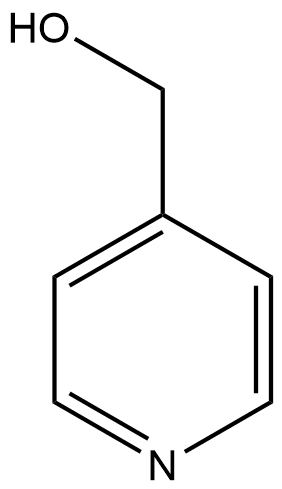
\includegraphics[scale=0.30]{figures/4HOMP.png}}
\quad
\subfigure[]{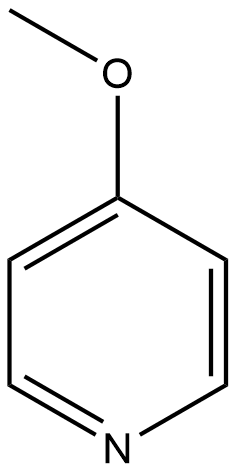
\includegraphics[scale=0.30]{figures/4-MOP.png}}
\caption{4-hydroxy-methyl-pyridine (a) and 4-methoxy-pyridine (b)}
\label{fig:4mophomp}
\end{figure}

The aim of this master thesis was the synthesis, spectral and structural characterization of new transition metal complexes using aforementioned pyridines with pseudohalides and transition metals.
Pseudohalides were chosen  as anionic ligands due to their similar properties to halides.  The central metal can bind to the end or middle atoms of these polyatomic ligands, making various combinations possible.\\

Mixing ligands and metal salts with varying ratios results in complexes with different coordination numbers (CN). Coordination numbers describe the number of donor atoms contained by ligands which are surrounding the central atom. 2, 4, 5 and 6 are common coordination numbers.\\

For the coordination number 2 only linear arrangements are  known and these complexes are often formed with the single positively charged ions \ce{Ag^+}, \ce{Cu^+} and \ce{Au^+}. \cite{riedel} \\

Tetrahedral and square-planar arrangements are possible for coordination number 4. Tetrahedral complexes are more common and are formed in all kinds of d-configurations whereas d$^8$-configuration (or 16-electron-complexes) prefer the square planar arrangement, i.e. \ce{Pt^{2+}} or \ce{Pd^{2+}}. \cite{riedel}   \\

Square-pyramidal and trigonal-bipyramidal structures are forms of the seldom appearing coordination number 5. They can be transformed into each other via Berry rotation \cite{berry} and are in equilibirium at a certain temperature.

CN 6 forms are octahedron (common), trigonal antiprism or trigonal prism (rare). The metal ions \ce{Cr^{3+}}, \ce{Co^{3+}} and  \ce{Pt^{3+}} favor the octahedral arrangement.\cite{riedel} \\

 
 The coordination numbers with their frequent arrangements are listed in figure \ref{fig:kz}.

\begin{figure}
\centering
\subfigure[CN2: linear]{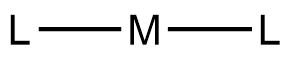
\includegraphics[width=0.30\linewidth]{figures/linear.png}}
\subfigure[CN4: square-planar]{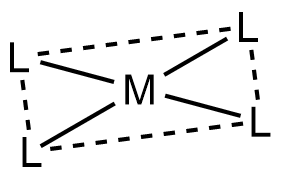
\includegraphics[width=0.30\linewidth]{figures/square-planar.png}}
\subfigure[CN4: tetrahedral]{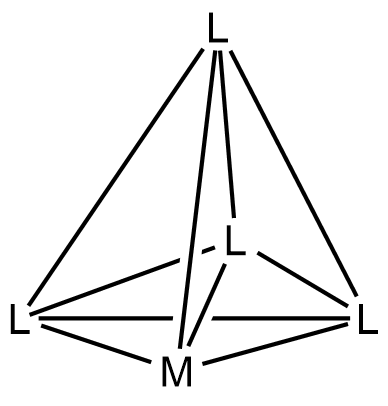
\includegraphics[width=0.30\linewidth]{figures/tetrahedral.png}}

\subfigure[CN5: square-pyramidal]{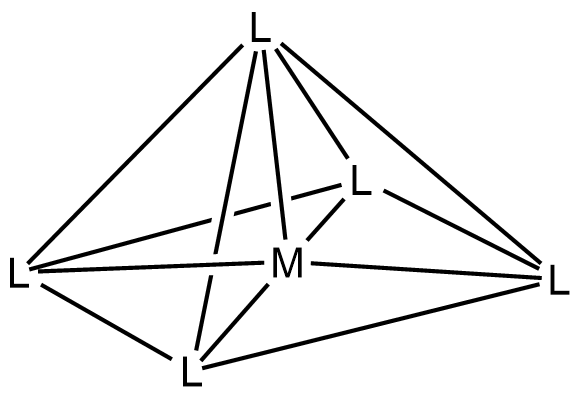
\includegraphics[width=0.30\linewidth]{figures/square-pyramidal.png}}
\subfigure[CN5: trigonal-bipyramidal]{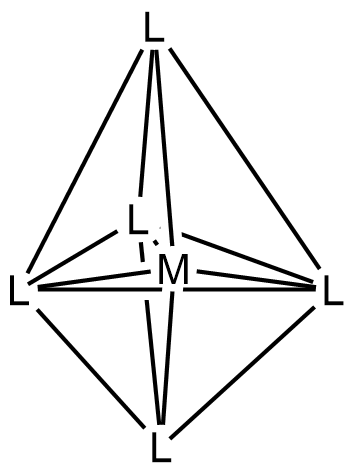
\includegraphics[width=0.30\linewidth]{figures/trigonal-bipyramidal.png}}
\subfigure[CN6: octahedral]{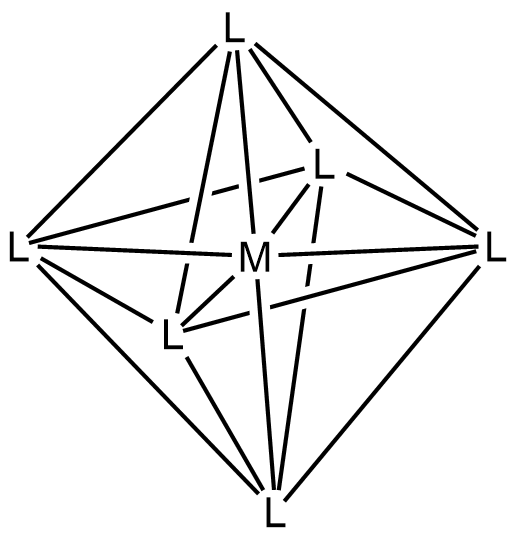
\includegraphics[width=0.30\linewidth]{figures/octahedral.png}}
\caption[Common structures of CNs]{Common structures of coordination numbers.}
\label{fig:kz}
\end{figure}+, \verb+\include{evaluation}+, \ldots)
%doc%   \end{itemize}
%doc% \item Create the \TeX{} files and fill your content into these files you defined in the previous step.
%doc% \item Optionally: Modify \myfile{colophon.tex} to meet your situation.
%doc%   \begin{itemize}
%doc%   \item Please spend a couple of minutes and think about putting your work
%doc%         under an open license\footnote{\url{https://creativecommons.org/licenses/}}
%doc%         in order to follow the spirit of Open Science\footnote{\url{https://en.wikipedia.org/wiki/Open_science}}.
%doc%   \end{itemize}
%doc% \item In case you are using \myacro{GNU} make\footnote{If you
%doc%       don't know, what \myacro{GNU} make is, you are not using it (yet).}:
%doc%       Put your desired \myacro{PDF} file name in the second line of file
%doc%    \myfile{Makefile}
%doc%    \begin{itemize}
%doc%    \item replace \enquote{Projectname} with your filename
%doc%    \item do not use any file extension like \texttt{.tex} or \texttt{.pdf}
%doc%    \end{itemize}
%doc% \end{enumerate}
%doc%
%doc%

%doc%
%doc% \subsection{License}\myimportant
%doc% \label{sec:license}
%doc%
%doc% This template is licensed under a Creative Commons Attribution-ShareAlike 3.0 Unported (CC BY-SA 3.0)
%doc%         license\footnote{\url{https://creativecommons.org/licenses/by-sa/3.0/}}:
%doc%     \begin{itemize}
%doc%     \item You can share (to copy, distribute and transmit) this template.
%doc%     \item You can remix (adapt) this template.
%doc%     \item You can make commercial use of the template.
%doc%     \item In case you modify this template and share the derived
%doc%           template: You must attribute the template such that you do not
%doc%           remove (co-)authorship of Karl Voit and you must not remove
%doc%           the URL to the original repository on
%doc%           github\footnote{\url{https://github.com/novoid/LaTeX-KOMA-template}}.
%doc%     \item If you alter, transform, or build a new template upon
%doc%           this template, you may distribute the resulting
%doc%           template only under the same or similar license to this one.
%doc%     \item There are \emph{no restrictions} of any kind, however, related to the
%doc%           resulting (PDF) document!
%doc%     \item You may remove the colophon (but it's not recommended).
%doc%     \end{itemize}


%doc%
%doc%
%doc% \subsection{How to compile this document}\myimportant
%doc% \label{sec:howtocompile}
%doc%
%doc% I assume that compiling \LaTeX{} documents within your software
%doc% environment is something you have already learned. This template is
%doc% almost like any other \LaTeX{} document except it uses
%doc% state-of-the-art tools for generating things like the list of
%doc% references using biblatex/biber (see
%doc% Section~\ref{sec:references} for details). Unfortunately, some \LaTeX{} editors
%doc% do not support this much better way of working with bibliography
%doc% references yet. This section describes how to compile this template.
%doc%
%doc% \subsubsection{Compiling Using a \LaTeX{} Editor}
%doc%
%doc% Please do select \myfile{main.tex} as the \enquote{main project file} or make
%doc% sure to compile/run only \myfile{main.tex} (and not \myfile{introduction.tex}
%doc% or other \TeX{} files of this template).
%doc%
%doc% Choose \texttt{biber} for generating the references. Modern LaTeX{}
%doc% environments offer this option. Older tools might not be that up to
%doc% date yet.
%doc%

%doc% \subsubsection{Activating \texttt{biber} in the \LaTeX{} editor TeXworks}
%doc% \label{sec:biberTeXworks}
%doc%
%doc% The \href{https://www.tug.org/texworks/}{TeXworks} editor is a very
%doc% basic (but fine) \LaTeX{} editor to start with. It is included in
%doc% \href{http://miktex.org/}{MiKTeX} and
%doc% \href{http://miktex.org/portable}{MiKTeX portable} and supports
%doc% \href{https://en.wikipedia.org/wiki/Syntax_highlighting}{syntax
%doc%   highlighting} and
%doc% \href{http://itexmac.sourceforge.net/SyncTeX.html}{SyncTeX} to
%doc% synchronize \myacro{PDF} output and \LaTeX{} source code.
%doc%
%doc% Unfortunately, TeXworks shipped with MiKTeX does not support compiling
%doc% using \texttt{biber} (biblatex) out of the box. Here is a solution to
%doc% this issue. Go to TeXworks: \texttt{Edit} $\rightarrow$
%doc% \texttt{Preferences~\ldots} $\rightarrow$ \texttt{Typesetting} $\rightarrow$
%doc% \texttt{Processing tools} and add a new entry (using the plus icon):
%doc%
%doc% \begin{tabbing}
%doc%   Arguments: \= foobar  \kill
%doc%   Name:      \> \verb#pdflatex+biber# \\
%doc%   Program:   \> \emph{find the \texttt{template/pdflatex+biber.bat} file from your disk} \\
%doc%   Arguments: \> \verb+$fullname+ \\
%doc%              \> \verb+$basename+
%doc% \end{tabbing}
%doc%
%doc% Activate the \enquote{View PDF after running} option.
%doc%
%doc% Close the preferences dialog and you will now have an additional
%doc% choice in the drop down list for compiling your document. Choose the
%doc% new entry called \verb#pdflatex+biber# and start a happier life with
%doc% \texttt{biber}.
%doc%
%doc% In case your TeXworks has a German user interface, here the key
%doc% aspects in German as well:
%doc%
%doc% \begin{otherlanguage}{ngerman}
%doc%
%doc%   \texttt{Bearbeiten} $\rightarrow$ \texttt{Einstellungen~\ldots} $\rightarrow$
%doc%   \texttt{Textsatz} $\rightarrow$ \texttt{Verarbeitungsprogramme} $\rightarrow$
%doc%   + \emph{(neues Verarbeitungsprogramm)}:
%doc%
%doc% \begin{tabbing}
%doc%   Befehl/Datei: \= foobar  \kill
%doc%     Name: \> pdflatex+biber \\
%doc%     Befehl/Datei: \> \emph{die \texttt{template/pdflatex+biber.bat} im Laufwerk suchen} \\
%doc%     Argumente: \> \verb+$fullname+ \\
%doc%                \> \verb+$basename+
%doc% \end{tabbing}
%doc%
%doc% \enquote{PDF nach Beendigung anzeigen} aktivieren.
%doc%
%doc% \end{otherlanguage}
%doc%

%doc% \subsubsection{Compiling Using \myacro{GNU} make}
%doc%
%doc% With \myacro{GNU}
%doc% make\footnote{\url{https://secure.wikimedia.org/wikipedia/en/wiki/Make\_\%28software\%29}}
%doc% it is just simple as that: \texttt{make pdf}
%doc%
%doc% Several other targets are available. You can check them out by
%doc% executing: \texttt{make help}
%doc%
%doc% In case you are using TeXLive (instead of MiKTeX as I do), you might
%doc% want to modify the line \texttt{PDFLATEX\_CMD = pdflatex} within
%doc% the file \texttt{Makefile} to: \texttt{PDFLATEX\_CMD = pdflatex -synctex=1 -undump=pdflatex}
%doc%
%doc%

%doc% \subsubsection{Compiling in a Text-Shell}
%doc%
%doc% To generate a document using \texttt{Biber}, you can stick to
%doc% following example:
%doc% \begin{verbatim}
%doc% pdflatex main.tex
%doc% biber main
%doc% pdflatex main.tex
%doc% pdflatex main.tex
%doc% \end{verbatim}
%doc% 
%doc% Users of TeXLive with Microsoft Windows might want to try the
%doc% following script\footnote{Thanks to Florian Brucker for provinding
%doc%   this script.} which could be stored as, e.g., \texttt{compile.bat}:
%doc% \begin{verbatim}
%doc% REM call pdflatex using parameters suitable for TeXLive:
%doc% pdflatex.exe  "main.tex"
%doc% REM generate the references metadata for biblatex (using biber):
%doc% biber.exe "main"
%doc% REM call pdflatex twice to compile the references and finalize PDF:
%doc% pdflatex.exe  "main.tex"
%doc% pdflatex.exe -synctex=-1 -interaction=nonstopmode "main.tex"
%doc% \end{verbatim}
%doc% 


%doc%
%doc% \subsection{How to get rid of the template documentation}
%doc%
%doc% Simply remove the files \verb#Template_Documentation.pdf# and
%doc% \verb#Template_Documentation.tex# (if it exists) in the main folder
%doc% of this template.
%doc%
%doc% \subsection{What about modifying or extending the template?}\myinteresting
%doc% \label{sec:extending-template}
%doc%
%doc% This template provides an easy to start \LaTeX{} document template with sound
%doc% default settings. You can modify each setting any time. It is recommended that
%doc% you are familiar with the documentation of the command whose settings you want
%doc% to modify.
%doc%
%doc% It is recommended that for \emph{adding} things to the preambel (newcommands,
%doc% setting variables, defining headers, \dots) you should use the file
%doc% \texttt{main.tex}.
%doc% There are comment lines which help you find the right spot.
%doc% This way you still have the chance to update your \texttt{template}
%doc% folder from the template repository without losing your own added things.
%doc%
%doc% The following sections describe the settings and commands of this template and
%doc% give a short overview of its features.

%doc% \subsection{How to change the title page}
%doc%
%doc% This template comes with a variety of title pages. They are located in
%doc% the folder \texttt{template}. You can switch to a specific title
%doc% page by including the corresponding title page file in the file
%doc% \texttt{main.tex}.
%doc%
%doc% Please note that you may not need to modify any title page document by
%doc% yourself since all relevant information is defined in the file
%doc% \texttt{main.tex}.

%doc%
%doc% \section{\texttt{preamble.tex} --- Main preamble file}
%doc%
%doc% In the file \verb#preamble/preamble.tex# you will find the basic
%doc% definitions related to your document. This template uses the \myacro{KOMA} script
%doc% extension package of \LaTeX{}.
%doc%
%doc% There are comments added to the \verb#\documentclass{}# definitions. Please
%doc% refer to the great documentation of \myacro{KOMA}\footnote{\texttt{scrguide.pdf} for
%doc% German users} for further details.
%doc%
%doc% \paragraph{What should I do with this file?} For standard purposes you might
%doc% use the default values it provides. You must not remove its \texttt{include} command
%doc% in \texttt{main.tex} since it contains important definitions. This file contains
%doc% settings which are documented well and can be modified according to your needs.
%doc% It is recommended that you fully understand each setting you modify in order to
%doc% get a good document result. However, you can set basic values in the
%doc% \texttt{main.tex} file: font size, paper size,
%doc% paragraph separation mode, draft mode, binding correction, and whether
%doc% your document will be a one sided document or you are planning to
%doc% create a document which is printed on both, left side and right side.
%doc%

\documentclass[%
fontsize=\myfontsize,%% size of the main text
paper=\mypapersize,  %% paper format
parskip=\myparskip,  %% vertical space between paragraphs (instead of indenting first par-line)
DIV=calc,            %% calculates a good DIV value for type area; 66 characters/line is great
headinclude=true,    %% is header part of margin space or part of page content?
footinclude=false,   %% is footer part of margin space or part of page content?
open=right,          %% "right" or "left": start new chapter on right or left page
appendixprefix=true, %% adds appendix prefix; only for book-classes with \backmatter
bibliography=totoc,  %% adds the bibliography to table of contents (without number)
draft=\mydraft,      %% if true: included graphics are omitted and black boxes
                     %%          mark overfull boxes in margin space
BCOR=\myBCOR,        %% binding correction (depends on how you bind
                     %% the resulting printout.
\mylaterality        %% oneside: document is not printed on left and right sides, only right side
                     %% twoside: document is printed on left and right sides
]{scrbook}  %% article class of KOMA: "scrartcl", "scrreprt", or "scrbook".
            %% CAUTION: If documentclass will be changed, *many* other things
            %%          change as well like heading structure, ...



% FIXXME: adopting class usage:
% from scrbook -> scrartcl OR scrreport:
% - remove appendixprefix from class options
% - remove \frontmatter \mainmatter \backmatter \appendix from main.tex

% FIXXME: adopting language:
% add or modify language parameter of package »babel« and use language switches described in babel-documentation

%doc%
%doc% \subsection{\texttt{inputenc}: UTF8 as input charset}
%doc%
%doc% You are able and should use \myacro{UTF8} character settings for writing these \TeX{}-files.
%doc%
%\usepackage{ucs}             %% UTF8 as input characters; UCS incompatible to biblatex
\usepackage[utf8]{inputenc} %% UTF8 as input characters
%% Source: http://latex.tugraz.at/latex/tutorial#laden_von_paketen


%doc%
%doc% \subsection{\texttt{babel}: Language settings}
%doc%
%doc% The default setting of the language is American. Please change settings for
%doc% additional or alternative languages used in \texttt{main.tex}.
%doc%
%doc% Please note that the default language of the document is the \emph{last} language
%doc% which is added to the package options.
%doc%
%doc% To set only parts of your document in a different language as the rest, use for example\newline
%doc% \verb+\foreignlanguage{ngerman}{Beispieltext in deutscher Sprache}+\newline
%doc% For using foreign language quotes, please refer to the \verb+\foreignquote+,
%doc% \verb+\foreigntextquote+, or \verb+\foreignblockquote+ provided by
%doc% \texttt{csquotes} (see Section~\ref{sub:csquotes}).
%doc%
\usepackage[\mylanguage]{babel}  %% used languages; default language is *last* language of options

%doc%
%doc% \subsection{\texttt{scrpage2}: Headers and footers}
%doc%
%doc% Since this template is based on \myacro{KOMA} script it uses its great \texttt{scrpage2}
%doc% package for defining header and footer information. Please refer to the \myacro{KOMA}
%doc% script documentation how to use this package.
%doc%
\usepackage{scrpage2} %%  advanced page style using KOMA


%doc%
%doc% \subsection{References}\myimportant
%doc% \label{sec:references}
%doc%
%doc% This template is using
%doc% \href{http://www.tex.ac.uk/tex-archive/info/translations/biblatex/de/}{\texttt{biblatex}}
%doc% and \href{http://en.wikipedia.org/wiki/Biber_(LaTeX)}{\texttt{Biber}}
%doc% instead of
%doc% \href{http://en.wikipedia.org/wiki/BibTeX}{\textsc{Bib}\TeX{}}. This has the following
%doc% advantages:
%doc% \begin{itemize}
%doc% \item better documentation
%doc% \item Unicode-support like German umlauts (ö, ä, ü, ß) for references
%doc% \item flexible definition of citation styles
%doc% \item multiple bibliographies e.\,g. for printed and online resources
%doc% \item cleaner reference definition e.\,g. inheriting information from
%doc%   \texttt{Proceedings} to all related \texttt{InProceedings}
%doc% \item modern implementation
%doc% \end{itemize}
%doc%
%doc% In short, \texttt{biblatex} is able to handle your \texttt{bib}-files
%doc% and offers additional features. To get the most out of
%doc% \texttt{biblatex}, you should read the very good package
%doc% documentation. Be warned: you'll probably never want to change back
%doc% to \textsc{Bib}\TeX{} again.
%doc%
%doc% Take a look at the files \texttt{references-bibtex.bib} and
%doc% \texttt{references-biblatex.bib}: they contain the three
%doc% references \texttt{tagstore}, \texttt{Voit2009}, and
%doc% \texttt{Voit2011}.
%doc% The second file is optimized for \texttt{biblatex} and
%doc% takes advantage of some features that are not possible with
%doc% \textsc{Bib}\TeX{}.
%doc%
%doc% This template is ready to use \texttt{biblatex} with \texttt{Biber} as
%doc% reference compiler. You should make sure that you have installed an up
%doc% to date binary of \texttt{Biber} from its
%doc% homepage\footnote{\url{http://biblatex-biber.sourceforge.net/}}.
%doc%
%doc%
%doc% In \texttt{main.tex} you can define several general \texttt{biblatex}
%doc% options: citation style, whether or not multiple occurrences of
%doc% authors are replaced with dashes, or if backward references (from
%doc% references to citations) should be added.
%doc%
%doc%
%doc% If you are using the LaTeX{} editor TeXworks, please make sure that
%doc% you have read Section~\ref{sec:biberTeXworks} in order to use
%doc% \texttt{biber}.
%doc%

%doc% \subsubsection{Example citation commands}
%doc%
%doc% This section demonstrates some example citations using the style \texttt{authoryear}.
%doc% You can change the citation style in \texttt{main.tex} (\texttt{mybiblatexstyle}).
%doc%
%doc% \begin{itemize}
%doc% \item cite \cite{Eijkhout2008} and cite \cite{Bringhurst1993, Eijkhout2008}.
%doc% \item citet \citet{Eijkhout2008} and citet \citet{Bringhurst1993, Eijkhout2008}.
%doc% \item autocite \autocite{Eijkhout2008} and autocite \autocite{Bringhurst1993, Eijkhout2008}.
%doc% \item autocites \autocites{Eijkhout2008} and autocites \autocites{Bringhurst1993, Eijkhout2008}.
%doc% \item citeauthor \citeauthor{Eijkhout2008} and citeauthor \citeauthor{Bringhurst1993, Eijkhout2008}.
%doc% \item citetitle \citetitle{Eijkhout2008} and citetitle \citetitle{Bringhurst1993, Eijkhout2008}.
%doc% \item citeyear \citeyear{Eijkhout2008} and citeyear \citeyear{Bringhurst1993, Eijkhout2008}.
%doc% \item textcite \textcite{Eijkhout2008} and textcite \textcite{Bringhurst1993, Eijkhout2008}.
%doc% \item smartcite \smartcite{Eijkhout2008} and smartcite \smartcite{Bringhurst1993, Eijkhout2008}.
%doc% \item footcite \footcite{Eijkhout2008} and footcite \footcite{Bringhurst1993, Eijkhout2008}.
%doc% \item footcite with page \footcite[p.42]{Eijkhout2008} and footcite with page \footcite[compare][p.\,42]{Eijkhout2008}.
%doc% \item fullcite \fullcite{Eijkhout2008} and fullcite \fullcite{Bringhurst1993, Eijkhout2008}.
%doc% \end{itemize}
%doc%
%doc% Please note that the citation style as well as the bibliography style
%doc% can be changed very easily. Refer to the settings in
%doc% \texttt{main.tex} as well as the very good documentation of \texttt{biblatex}.
%doc%

%doc% \subsubsection{Using this template with \myacro{APA} style}
%doc%
%doc% First, you have to have the \myacro{APA} biblatex style
%doc% installed. Modern \LaTeX{} distributions do come with
%doc% \texttt{biblatex} and \myacro{APA} style. If so, you will find the
%doc% files \texttt{biblatex-apa.pdf} (style documentation) and
%doc% \texttt{biblatex-apa-test.pdf} (file with citation examples) on your
%doc% hard disk.
%doc%
%doc% \begin{enumerate}
%doc% \item Change the style according to \verb#\newcommand{\mybiblatexstyle}{apa}#
%doc% \item Add \verb#\DeclareLanguageMapping{american}{american-apa}# or \\
%doc%   \verb#\DeclareLanguageMapping{german}{german-apa}# to your
%doc%   preamble\footnote{You might want to use section \enquote{MISC
%doc%       self-defined commands and settings} for this.}
%doc% \end{enumerate}
%doc%
%doc% These steps change the biblatex style to \myacro{APA} style

%doc%
%doc% \subsubsection{Using this template with \textsc{Bib}\TeX{}}
%doc%
%doc% If you do not want to use \texttt{Biber} and \texttt{biblatex}, you
%doc% have to change several things:
%doc% \begin{itemize}
%doc% \item in \verb#preamble/preamble.tex#
%doc%   \begin{itemize}
%doc%   \item remove the usepackage command of \texttt{biblatex}
%doc%   \item remove the \verb#\addbibresource{...}# command
%doc%   \end{itemize}
%doc% \item in \verb#main.tex#
%doc%   \begin{itemize}
%doc%   \item replace \verb=\printbibliography= with the usual
%doc%     \verb=\bibliographystyle{yourstyle}= and \verb=\bibliography{yourbibfile}=
%doc%   \end{itemize}
%doc% \item if you are using \myacro{GNU} \texttt{make}: modify \verb=Makefile=
%doc%   \begin{itemize}
%doc%   \item replace \verb#BIBTEX_CMD = biber# with \verb#BIBTEX_CMD = bibtex#
%doc%   \end{itemize}
%doc% \item Use the reference file \texttt{references-bibtex.bib}
%doc%   instead of \texttt{references-biblatex.bib}
%doc% \end{itemize}
%doc%
%doc%
\usepackage[backend=biber, %% using "biber" to compile references (instead of "biblatex")
style=\mybiblatexstyle, %% see biblatex documentation
%style=alphabetic, %% see biblatex documentation
maxbibnames=1000,
backref=\mybiblatexbackref, %% create backlings from references to citations
natbib=true, %% offering natbib-compatible commands
hyperref=true, %% using hyperref-package references
sorting=none
]{biblatex}  %% remove, if using BibTeX instead of biblatex

\addbibresource{\mybiblatexfile} %% remove, if using BibTeX instead of biblatex



%doc%
%doc% \subsection{Miscellaneous packages} \label{subsec:miscpackages}
%doc%
%doc% There are several packages included by default. You might want to activate or
%doc% deactivate them according to your requirements:
%doc%
%doc% \begin{enumerate}

%doc% \item[\texttt{\href{http://www.ctan.org/pkg/graphicx}{%%
%doc% graphicx%%
%doc% }}]
%doc% The widely used package to use graphical images within a \LaTeX{} document.
\usepackage[pdftex]{graphicx}

%doc% \item[\texttt{\href{https://secure.wikimedia.org/wikibooks/en/wiki/LaTeX/Formatting\#Other\_symbols}{%%
%doc% pifont%%
%doc% }}]
%doc% For additional special characters available by \verb#\ding{}#
\usepackage{pifont}


%doc% \item[\texttt{\href{http://ctan.org/pkg/ifthen}{%%
%doc% ifthen%%
%doc% }}]
%doc% For using if/then/else statements for example in macros
\usepackage{ifthen}

%% pre-define ifthen-boolean variables:
\newboolean{myaddcolophon}
\newboolean{myaddlistoftodos}


%doc% \item[\texttt{\href{http://www.ctan.org/tex-archive/fonts/eurosym}{%%
%doc% eurosym%%
%doc% }}]
%doc% Using the character for Euro with \verb#\officialeuro{}#
%\usepackage{eurosym}

%doc% \item[\texttt{\href{http://www.ctan.org/tex-archive/help/Catalogue/entries/xspace.html}{%%
%doc% xspace%%
%doc% }}]
%doc% This package is required for intelligent spacing after commands
\usepackage{xspace}

%doc% \item[\texttt{\href{https://secure.wikimedia.org/wikibooks/en/wiki/LaTeX/Colors}{%%
%doc% xcolor%%
%doc% }}]
%doc% This package defines basic colors. If you want to get rid of colored links and headings
%doc% please change corresponding value in \texttt{main.tex} to \{0,0,0\}.
\usepackage[usenames,dvipsnames]{xcolor}
\definecolor{DispositionColor}{RGB}{\mydispositioncolor} %% used for links and so forth in screen-version

%doc% \item[\texttt{\href{http://www.ctan.org/pkg/ulem}{%%
%doc% ulem%%
%doc% }}]
%doc% This package offers strikethrough command \verb+\sout{foobar}+.
\usepackage[normalem]{ulem}

%doc% \item[\texttt{\href{http://www.ctan.org/pkg/framed}{%%
%doc% framed%%
%doc% }}]
%doc% Create framed, shaded, or differently highlighted regions that can
%doc% break across pages.  The environments defined are
%doc% \begin{itemize}
%doc%   \item framed: ordinary frame box (\verb+\fbox+) with edge at margin
%doc%   \item shaded: shaded background (\verb+\colorbox+) bleeding into margin
%doc%   \item snugshade: similar
%doc%   \item leftbar: thick vertical line in left margin
%doc% \end{itemize}
\usepackage{framed}

%doc% \item[\texttt{\href{http://www.ctan.org/pkg/eso-pic}{%%
%doc% eso-pic%%
%doc% }}]
%doc% For example on title pages you might want to have a logo on the upper right corner of
%doc% the first page (only). The package \texttt{eso-pic} is able to place things on absolute
%doc% and relative positions on the whole page.
\usepackage{eso-pic}

%doc% \item[\texttt{\href{http://ctan.org/pkg/enumitem}{%%
%doc% enumitem%%
%doc% }}]
%doc% This package replaces the built-in definitions for enumerate, itemize and description.
%doc% With \texttt{enumitem} the user has more control over the layout of those environments.
\usepackage{enumitem}

%doc% \item[\texttt{\href{http://www.ctan.org/tex-archive/macros/latex/contrib/todonotes/}{%%
%doc% todonotes%%
%doc% }}]
%doc% This packages is \emph{very} handy to add notes\footnote{\texttt{todonotes} replaced
%doc% the \texttt{fixxme}-command which previously was defined in the
%doc% \texttt{preamble\_mycommands.tex} file.}. Using for example \verb#\todo{check}#
%doc% results in something like this \todo{check} in the document. Do read the
%doc% great package documentation for usage of other very helpful commands such as
%doc% \verb#\missingfigure{}# and \verb#\listoftodos#. The latter one creates an index of all
%doc% open todos which is very useful for getting an overview of open issues.
%doc% The package \texttt{todonotes} require the packages \texttt{ifthen}, \texttt{xkeyval}, \texttt{xcolor},
%doc% \texttt{tikz}, \texttt{calc}, and \texttt{graphicx}. Activate
%doc% and configure \verb#\listoftodos# in \texttt{main.tex}.
%\usepackage{todonotes}
\usepackage[\mytodonotesoptions]{todonotes}  %% option "disable" removes all todonotes output from resulting document

%disabled% \item[\texttt{\href{http://www.ctan.org/tex-archive/macros/latex/contrib/blindtext}{%%
%disabled% blindtext%%
%disabled% }}]
%disabled% This package is used to generate blind text for demonstration purposes.
%disabled% %% This is undocumented due to problems using american english; author informed
%disabled% \usepackage{blindtext}  %% provides commands for blind text:
%disabled% %% \blindtext creates some text,
%disabled% %% \Blindtext creates more text.
%disabled% %% \blinddocument creates a small document with sections, lists...
%disabled% %% \Blinddocument creates a large document with sections, lists...
%% 2012-03-10: vk: author published a corrected version which is able to handle "american english" as well. Did not have time to check new package version for this template here.

%doc% \item[\texttt{\href{http://ctan.org/tex-archive/macros/latex/contrib/units}{%%
%doc% units%%
%doc% }}]
%doc% For setting correctly typesetted units and nice fractions with \verb+\unit[42]{m}+ and \verb+\unitfrac[100]{km}{h}+.
\usepackage{units}


%doc% \end{enumerate}




%%%% End
%%% Local Variables:
%%% TeX-master: "../main"
%%% mode: latex
%%% mode: auto-fill
%%% mode: flyspell
%%% eval: (ispell-change-dictionary "en_US")
%%% End:
%% vim:foldmethod=expr
%% vim:fde=getline(v\:lnum)=~'^%%%%'?0\:getline(v\:lnum)=~'^%doc.*\ .\\%(sub\\)\\?section{.\\+'?'>1'\:'1':
%% DO NOT REMOVE THIS LINE!

\setboolean{myaddcolophon}{false}  %% "true" or "false"
%% If set to "true": a colophon (with notes about this document
%% template, LaTeX, ...) is added after the title page.
%% Please do not set to "false" without a good reason. The colophon
%% helps your readers to get in touch with LaTeX and to find this template.

\setboolean{myaddlistoftodos}{false}  %% "true" or "false"
%% If set to "true": the current list of open todos is added after the
%% table of contents. If \mytodonotesoptions is set to "disable", no
%% list of todos is added, independent of this setting here.



%% ========================================================================
%%%% Document metadata
%% ========================================================================

%% general metadata:
\newcommand{\myauthor}{Magdalena Traber}  %% also used for PDF metadata (hyperref)
\newcommand{\mytitle}{Synthesis and structural characterization of pseudohalide complexes with 4-hydroxymethylpyridine and 4-methoxypyridine as coligands}  %% also used for PDF metadata (hyperref)
\newcommand{\mysubject}{SUBJECT}  %% also used for PDF metadata (hyperref)
\newcommand{\mykeywords}{KEYWORDS}  %% also used for PDF metadata (hyperref)

%% this information is used only for generating the title page:
\newcommand{\myworktitle}{Master's Thesis}  %% official type of work like ``Master theses''
\newcommand{\mygrade}{Master of Science} %% title you are getting with this work like ``Master of ...''
\newcommand{\mystudy}{Chemistry} %% your study like ``Arts''
\newcommand{\myuniversity}{Graz University of Technology} %% your university/school
\newcommand{\myinstitute}{Institute of Physical and Theoretical Chemistry} %% affiliation
\newcommand{\myinstitutehead}{Univ.-Prof Mag.rer.nat. Dr.phil. Georg Gescheidt-Demner} %% head of institute
\newcommand{\mysupervisor}{Ao.Univ.-Prof. Dipl.Ing. Dr.techn. Franz-Andreas Mautner} %% your supervisor
\newcommand{\myevaluator}{Ao.Univ.-Prof. Dipl.Ing. Dr.techn. Franz-Andreas Mautner} %% your evaluator
\newcommand{\myhomestreet}{Zwerggasse 7/3} %% your home street (with house number)
\newcommand{\myhometown}{Graz} %% your home town
\newcommand{\myhomepostalnumber}{8010} %% your postal number of home town
\newcommand{\mysubmissionmonth}{April} %% month you are handing in
\newcommand{\mysubmissionyear}{2017} %% year you are handing in
\newcommand{\mysubmissiontown}{\myhometown} %% town of handing in (or \myhometown)

%% additional information for generic_documentation title page
\newcommand{\myid}{1010067} %% Matrikelnummer
\newcommand{\mylecture}{LECTURE} %%


%% ========================================================================
%%%% MISC command definitions
%% ========================================================================
%% Time-stamp: <2015-04-30 17:19:58 vk>
%%%% === Disclaimer: =======================================================
%% created by
%%
%%      Karl Voit
%%
%% using GNU/Linux, GNU Emacs & LaTeX 2e
%%

%doc%
%doc% \section{\texttt{mycommands.tex} --- various definitions}\myinteresting
%doc% \label{sec:mycommands}
%doc%
%doc% In file \verb#template/mycommands.tex# many useful commands are being
%doc% defined. 
%doc% 
%doc% \paragraph{What should I do with this file?} Please take a look at its 
%doc% content to get the most out of your document.
%doc% 

%doc% 
%doc% One of the best advantages of \LaTeX{} compared to \myacro{WYSIWYG} software products is
%doc% the possibility to define and use macros within text. This empowers the user to
%doc% a great extend.  Many things can be defined using \verb#\newcommand{}# and
%doc% automates repeating tasks. It is recommended to use macros not only for
%doc% repetitive tasks but also for separating form from content such as \myacro{CSS}
%doc% does for \myacro{XHTML}. Think of including graphics in your document: after
%doc% writing your book, you might want to change all captions to the upper side of
%doc% each figure. In this case you either have to modify all
%doc% \texttt{includegraphics} commands or you were clever enough to define something
%doc% like \verb#\myfig#\footnote{See below for a detailed description}. Using a
%doc% macro for including graphics enables you to modify the position caption on only
%doc% \emph{one} place: at the definition of the macro.
%doc% 
%doc% The following section describes some macros that came with this document template
%doc% from \myLaT and you are welcome to modify or extend them or to create
%doc% your own macros!
%doc% 

%doc% 
%doc% \subsection{\texttt{myfig} --- including graphics made easy}
%doc% 
%doc% The classic: you can easily add graphics to your document with \verb#\myfig#:
%doc% \begin{verbatim}
%doc%  \myfig{flower}%% filename w/o extension in the folder figures
%doc%        {width=0.7\textwidth}%% maximum width/height, aspect ratio will be kept
%doc%        {This flower was photographed at my home town in 2010}%% caption
%doc%        {Home town flower}%% optional (short) caption for list of figures
%doc%        {fig:flower}%% label
%doc% \end{verbatim}
%doc% 
%doc% There are many advantages of this command (compared to manual
%doc% \texttt{figure} environments and \texttt{includegraphics} commands:
%doc% \begin{itemize}
%doc% \item consistent style throughout the whole document
%doc% \item easy to change; for example move caption on top
%doc% \item much less characters to type (faster, error prone)
%doc% \item less visual clutter in the \TeX{}-files
%doc% \end{itemize}
%doc% 
%doc% 
\newcommand{\myfig}[5]{
%% example:
% \myfig{}%% filename in figures folder
%       {width=0.5\textwidth,height=0.5\textheight}%% maximum width/height, aspect ratio will be kept
%       {}%% caption
%       {}%% optional (short) caption for list of figures
%       {}%% label
\begin{figure}%[htp]
  \centering
  \includegraphics[keepaspectratio,#2]{figures/#1}
  \caption[#4]{#3}
  \label{#5} %% NOTE: always label *after* caption!
\end{figure}
}


%doc% 
%doc% \subsection{\texttt{myclone} --- repeat things!}
%doc% 
%doc% Using \verb#\myclone[42]{foobar}# results the text \enquote{foobar} printed 42 times.
%doc% But you can not only repeat text output with \texttt{myclone}. 
%doc%
%doc% Default argument
%doc% for the optional parameter \enquote{number of times} (like \enquote{42} in the example above) 
%doc% is set to two.
%doc% 
%% \myclone[x]{text}
\newcounter{myclonecnt}
\newcommand{\myclone}[2][2]{%
  \setcounter{myclonecnt}{#1}%
  \whiledo{\value{myclonecnt}>0}{#2\addtocounter{myclonecnt}{-1}}%
}

%old% %d oc% 
%old% %d oc% \subsection{\texttt{fixxme} --- sidemark something as unfinished}
%old% %d oc% 
%old% %d oc% You know it: something has to be fixed and you can not do it right
%old% %d oc% now. In order to \texttt{not} forget about it, you might want to add a
%old% %d oc% note like \verb+\fixxme{check again}+ which inserts a note on the page
%old% %d oc% margin such as this\fixxme{check again} example.
%old% %d oc%
%old% \newcommand{\fixxme}[1]{%%
%old% \textcolor{red}{FIXXME}\marginpar{\textcolor{red}{#1}}%%
%old% }


%%%% End 
%%% Local Variables:
%%% mode: latex
%%% mode: auto-fill
%%% mode: flyspell
%%% eval: (ispell-change-dictionary "en_US")
%%% TeX-master: "../main"
%%% End:
%% vim:foldmethod=expr
%% vim:fde=getline(v\:lnum)=~'^%%%%'?0\:getline(v\:lnum)=~'^%doc.*\ .\\%(sub\\)\\?section{.\\+'?'>1'\:'1':


%% ========================================================================
%%%% Typographic settings
%% ========================================================================
%%%% Time-stamp: <2015-08-22 17:20:32 vk>
%%%% === Disclaimer: =======================================================
%% created by
%%
%%      Karl Voit
%%
%% using GNU/Linux, GNU Emacs & LaTeX 2e
%%
%doc%
%doc% \section{\texttt{typographic\_settings.tex} --- Typographic finetuning}
%doc%
%doc% The settings of file \verb#template/typographic_settings.tex# contain
%doc% typographic finetuning related to things mentioned in literature.  The
%doc% settings in this file relates to personal taste and most of all: 
%doc% \emph{typographic experience}. 
%doc% 
%doc% \paragraph{What should I do with this file?} You might as well skip the whole
%doc% file by excluding the \verb#%%%% Time-stamp: <2015-08-22 17:20:32 vk>
%%%% === Disclaimer: =======================================================
%% created by
%%
%%      Karl Voit
%%
%% using GNU/Linux, GNU Emacs & LaTeX 2e
%%
%doc%
%doc% \section{\texttt{typographic\_settings.tex} --- Typographic finetuning}
%doc%
%doc% The settings of file \verb#template/typographic_settings.tex# contain
%doc% typographic finetuning related to things mentioned in literature.  The
%doc% settings in this file relates to personal taste and most of all: 
%doc% \emph{typographic experience}. 
%doc% 
%doc% \paragraph{What should I do with this file?} You might as well skip the whole
%doc% file by excluding the \verb#%%%% Time-stamp: <2015-08-22 17:20:32 vk>
%%%% === Disclaimer: =======================================================
%% created by
%%
%%      Karl Voit
%%
%% using GNU/Linux, GNU Emacs & LaTeX 2e
%%
%doc%
%doc% \section{\texttt{typographic\_settings.tex} --- Typographic finetuning}
%doc%
%doc% The settings of file \verb#template/typographic_settings.tex# contain
%doc% typographic finetuning related to things mentioned in literature.  The
%doc% settings in this file relates to personal taste and most of all: 
%doc% \emph{typographic experience}. 
%doc% 
%doc% \paragraph{What should I do with this file?} You might as well skip the whole
%doc% file by excluding the \verb#\input{template/typographic_settings.tex}# command
%doc% in \texttt{main.tex}.  For standard usage it is recommended to stay with the
%doc% default settings.
%doc% 
%doc% 
%% ========================================================================

%doc%
%doc% Some basic microtypographic settings are provided by the
%doc% \texttt{microtype}
%doc% package\footnote{\url{http://ctan.org/pkg/microtype}}. This template
%doc% uses the rather conservative package parameters: \texttt{protrusion=true,factor=900}.
\usepackage[protrusion=true,factor=900]{microtype}

%doc%
%doc% \subsection{French spacing}
%doc%
%doc% \paragraph{Why?} see~\textcite[p.\,28, p.\,30]{Bringhurst1993}: `2.1.4 Use a single word space between sentences.'
%doc%
%doc% \paragraph{How?} see~\textcite[p.\,185]{Eijkhout2008}:\\
%doc% \verb#\frenchspacing  %% Macro to switch off extra space after punctuation.# \\
\frenchspacing  %% Macro to switch off extra space after punctuation.
%doc%
%doc% Note: This setting might be default for \myacro{KOMA} script.
%doc%


%doc%
%doc% \subsection{Font}
%doc% 
%doc% This template is using the Palatino font (package \texttt{mathpazo}) which results
%doc% in a legible document and matching mathematical fonts for printout.
%doc% 
%doc% It is highly recommended that you either stick to the Palatino font or use the
%doc% \LaTeX{} default fonts (by removing the package \texttt{mathpazo}).
%doc% 
%doc% Chosing different fonts is not
%doc% an easy task. Please leave this to people with good knowledge on this subject.
%doc% 
%doc% One valid reason to change the default fonts is when your document is mainly
%doc% read on a computer screen. In this case it is recommended to switch to a font
%doc% \textsf{which is sans-serif like this}. This template contains several alternative
%doc% font packages which can be activated in this file.
%doc% 

% for changing the default font, please go to the next subsection!

%doc%
%doc% \subsection{Text figures}
%doc% 
%doc% \ldots also called old style numbers such as 0123456789. 
%doc% (German: \enquote{Mediäval\-ziffern\footnote{\url{https://secure.wikimedia.org/wikibooks/de/wiki/LaTeX-W\%C3\%B6rterbuch:\_Medi\%C3\%A4valziffern}}})
%doc% \paragraph{Why?} see~\textcite[p.\,44f]{Bringhurst1993}: 
%doc% \begin{quote}
%doc% `3.2.1 If the font includes both text figures and titling figures, use
%doc%  titling figures only with full caps, and text figures in all other
%doc%  circumstances.'
%doc% \end{quote}
%doc% 
%doc% \paragraph{How?} 
%doc% Quoted from Wikibooks\footnote{\url{https://secure.wikimedia.org/wikibooks/en/wiki/LaTeX/Formatting\#Text\_figures\_.28.22old\_style.22\_numerals.29}}:
%doc% \begin{quote}
%doc% Some fonts do not have text figures built in; the textcomp package attempts to
%doc% remedy this by effectively generating text figures from the currently-selected
%doc% font. Put \verb#\usepackage{textcomp}# in your preamble. textcomp also allows you to
%doc% use decimal points, properly formatted dollar signs, etc. within
%doc% \verb#\oldstylenums{}#.
%doc% \end{quote}
%doc% \ldots but proposed \LaTeX{} method does not work out well. Instead use:\\
%doc% \verb#\usepackage{hfoldsty}#  (enables text figures using additional font) or \\
%doc% \verb#\usepackage[sc,osf]{mathpazo}# (switches to Palatino font with small caps and old style figures enabled).
%doc%
%\usepackage{hfoldsty}  %% enables text figures using additional font
%% ... OR use ...
\usepackage[sc,osf]{mathpazo} %% switches to Palatino with small caps and old style figures

%% Font selection from:
%%     http://www.matthiaspospiech.de/latex/vorlagen/allgemein/preambel/fonts/
%% use following lines *instead* of the mathpazo package above:
%% ===== Serif =========================================================
%% for Computer Modern (LaTeX default font), simply remove the mathpazo above
%\usepackage{charter}\linespread{1.05} %% Charter
%\usepackage{bookman}                  %% Bookman (laedt Avant Garde !!)
%\usepackage{newcent}                  %% New Century Schoolbook (laedt Avant Garde !!)
%% ===== Sans Serif ====================================================
%\renewcommand{\familydefault}{\sfdefault}  %% this one in *combination* with the default mathpazo package
%\usepackage{cmbright}                  %% CM-Bright (eigntlich eine Familie)
%\usepackage{tpslifonts}                %% tpslifonts % Font for Slides


%doc% 
%doc% \subsection{\texttt{myacro} --- Abbrevations using \textsc{small caps}}\myinteresting
%doc% \label{sec:myacro}
%doc% 
%doc% \paragraph{Why?} see~\textcite[p.\,45f]{Bringhurst1993}: `3.2.2 For abbrevations and
%doc% acronyms in the midst of normal text, use spaced small caps.'
%doc% 
%doc% \paragraph{How?} Using the predefined macro \verb#\myacro{}# for things like
%doc% \myacro{UNO} or \myacro{UNESCO} using \verb#\myacro{UNO}# or \verb#\myacro{UNESCO}#.
%doc% 
\DeclareRobustCommand{\myacro}[1]{\textsc{\lowercase{#1}}} %%  abbrevations using small caps


%doc% 
%doc% \subsection{Colorized headings and links}
%doc% 
%doc% This document template is able to generate an output that uses colorized
%doc% headings, captions, page numbers, and links. The color named `DispositionColor'
%doc% used in this document is defined near the definition of package \texttt{color}
%doc% in the preamble (see section~\ref{subsec:miscpackages}). The changes required
%doc% for headings, page numbers, and captions are defined here.
%doc% 
%doc% Settings for colored links are handled by the definitions of the
%doc% \texttt{hyperref} package (see section~\ref{sec:pdf}).
%doc% 
\setheadsepline{.4pt}[\color{DispositionColor}]
\renewcommand{\headfont}{\normalfont\sffamily\color{DispositionColor}}
\renewcommand{\pnumfont}{\normalfont\sffamily\color{DispositionColor}}
\addtokomafont{disposition}{\color{DispositionColor}}
\addtokomafont{caption}{\color{DispositionColor}\footnotesize}
\addtokomafont{captionlabel}{\color{DispositionColor}}

%doc% 
%doc% \subsection{No figures or tables below footnotes}
%doc% 
%doc% \LaTeX{} places floating environments below footnotes if \texttt{b}
%doc% (bottom) is used as (default) placement algorithm. This is certainly
%doc% not appealing for most people and is deactivated in this template by
%doc% using the package \texttt{footmisc} with its option \texttt{bottom}.
%doc% 
%% see also: http://www.komascript.de/node/858 (German description)
\usepackage[bottom]{footmisc}

%doc% 
%doc% \subsection{Spacings of list environments}
%doc% 
%doc% By default, \LaTeX{} is using vertical spaces between items of enumerate, 
%doc% itemize and description environments. This is fine for multi-line items.
%doc% Many times, the user does just write single-line items where the larger
%doc% vertical space is inappropriate. The \href{http://ctan.org/pkg/enumitem}{enumitem}
%doc% package provides replacements for the pre-defined list environments and
%doc% offers many options to modify their appearances.
%doc% This template is using the package option for \texttt{noitemsep} which
%doc% mimimizes the vertical space between list items.
%doc% 
\usepackage{enumitem}
\setlist{noitemsep}   %% kills the space between items

%doc% 
%doc% \subsection{\texttt{csquotes} --- Correct quotation marks}\myinteresting
%doc% \label{sub:csquotes}
%doc% 
%doc% \emph{Never} use quotation marks found on your keyboard.
%doc% They end up in strange characters or false looking quotation marks.
%doc% 
%doc% In \LaTeX{} you are able to use typographically correct quotation marks. The package 
%doc% \href{http://www.ctan.org/pkg/csquotes}{\texttt{csquotes}} offers you with 
%doc% \verb#\enquote{foobar}# a command to get correct quotation marks around \enquote{foobar}.
%doc% Please do check the package options in order to modify
%doc% its settings according to the language used\footnote{most of the time in 
%doc% combination with the language set in the options of the \texttt{babel} package}.
%doc% 
%doc% \href{http://www.ctan.org/pkg/csquotes}{\texttt{csquotes}} is also recommended 
%doc% by \texttt{biblatex} (see Section~\ref{sec:references}). 
\usepackage[babel=true,strict=true,english=american,german=guillemets]{csquotes}

%doc% 
%doc% \subsection{Line spread}
%doc% 
%doc% If you have to enlarge the distance between two lines of text, you can
%doc% increase it using the \texttt{\mylinespread} command in \texttt{main.tex}. By default, it is
%doc% deactivated (set to 100~percent). Modify only with caution since it influences the
%doc% page layout and could lead to ugly looking documents.
\linespread{\mylinespread}

%doc% 
%doc% \subsection{Optional: Lines above and below the chapter head}
%doc% 
%doc% This is not quite something typographic but rather a matter of taste.
%doc% \myacro{KOMA} Script offers \href{http://www.komascript.de/node/24}{a method to
%doc% add lines above and below chapter head} which is disabled by
%doc% default. If you want to enable this feature, remove corresponding
%doc% comment characters from the settings.
%doc% 
%% Source: http://www.komascript.de/node/24
%disabled% %% 1st get a new command
%disabled% \newcommand*{\ORIGchapterheadstartvskip}{}%
%disabled% %% 2nd save the original definition to the new command
%disabled% \let\ORIGchapterheadstartvskip=\chapterheadstartvskip
%disabled% %% 3rd redefine the command using the saved original command
%disabled% \renewcommand*{\chapterheadstartvskip}{%
%disabled%   \ORIGchapterheadstartvskip
%disabled%   {%
%disabled%     \setlength{\parskip}{0pt}%
%disabled%     \noindent\color{DispositionColor}\rule[.3\baselineskip]{\linewidth}{1pt}\par
%disabled%   }%
%disabled% }
%disabled% %% see above
%disabled% \newcommand*{\ORIGchapterheadendvskip}{}%
%disabled% \let\ORIGchapterheadendvskip=\chapterheadendvskip
%disabled% \renewcommand*{\chapterheadendvskip}{%
%disabled%   {%
%disabled%     \setlength{\parskip}{0pt}%
%disabled%     \noindent\color{DispositionColor}\rule[.3\baselineskip]{\linewidth}{1pt}\par
%disabled%   }%
%disabled%   \ORIGchapterheadendvskip
%disabled% }

%doc% 
%doc% \subsection{Optional: Chapter thumbs}
%doc% 
%doc% This is not quite something typographic but rather a matter of taste.
%doc% \myacro{KOMA} Script offers \href{http://www.komascript.de/chapterthumbs-example}{a method to
%doc% add chapter thumbs} (in combination with the package \texttt{scrpage2}) which is disabled by
%doc% default. If you want to enable this feature, remove corresponding
%doc% comment characters from the settings.
%doc% 
%disabled% \makeatletter
%disabled% % Safty first
%disabled% \@ifundefined{chapter}{\let\chapter\undefined
%disabled%   \chapter must be defined to use chapter thumbs!}{%
%disabled%  
%disabled% % Two new commands for the width and height of the boxes with the
%disabled% % chapter number at the thumbs (use of commands instead of lengths
%disabled% % for sparing registers)
%disabled% \newcommand*{\chapterthumbwidth}{2em}
%disabled% \newcommand*{\chapterthumbheight}{1em}
%disabled%  
%disabled% % Two new commands for the colors of the box background and the
%disabled% % chapter numbers of the thumbs
%disabled% \newcommand*{\chapterthumbboxcolor}{black}
%disabled% \newcommand*{\chapterthumbtextcolor}{white}
%disabled%  
%disabled% % New command to set a chapter thumb. I'm using a group at this
%disabled% % command, because I'm changing the temporary dimension \@tempdima
%disabled% \newcommand*{\putchapterthumb}{%
%disabled%   \begingroup
%disabled%     \Large
%disabled%     % calculate the horizontal possition of the right paper border
%disabled%     % (I ignore \hoffset, because I interprete \hoffset moves the page
%disabled%     % at the paper e.g. if you are using cropmarks)
%disabled%     \setlength{\@tempdima}{\@oddheadshift}% (internal from scrpage2)
%disabled%     \setlength{\@tempdima}{-\@tempdima}%
%disabled%     \addtolength{\@tempdima}{\paperwidth}%
%disabled%     \addtolength{\@tempdima}{-\oddsidemargin}%
%disabled%     \addtolength{\@tempdima}{-1in}%
%disabled%     % putting the thumbs should not change the horizontal
%disabled%     % possition
%disabled%     \rlap{%
%disabled%       % move to the calculated horizontal possition
%disabled%       \hspace*{\@tempdima}%
%disabled%       % putting the thumbs should not change the vertical
%disabled%       % possition
%disabled%       \vbox to 0pt{%
%disabled%         % calculate the vertical possition of the thumbs (I ignore
%disabled%         % \voffset for the same reasons told above)
%disabled%         \setlength{\@tempdima}{\chapterthumbwidth}%
%disabled%         \multiply\@tempdima by\value{chapter}%
%disabled%         \addtolength{\@tempdima}{-\chapterthumbwidth}%
%disabled%         \addtolength{\@tempdima}{-\baselineskip}%
%disabled%         % move to the calculated vertical possition
%disabled%         \vspace*{\@tempdima}%
%disabled%         % put the thumbs left so the current horizontal possition
%disabled%         \llap{%
%disabled%           % and rotate them
%disabled%           \rotatebox{90}{\colorbox{\chapterthumbboxcolor}{%
%disabled%               \parbox[c][\chapterthumbheight][c]{\chapterthumbwidth}{%
%disabled%                 \centering
%disabled%                 \textcolor{\chapterthumbtextcolor}{%
%disabled%                   \strut\thechapter}\\
%disabled%               }%
%disabled%             }%
%disabled%           }%
%disabled%         }%
%disabled%         % avoid overfull \vbox messages
%disabled%         \vss
%disabled%       }%
%disabled%     }%
%disabled%   \endgroup
%disabled% }
%disabled%  
%disabled% % New command, which works like \lohead but also puts the thumbs (you
%disabled% % cannot use \ihead with this definition but you may change this, if
%disabled% % you use more internal scrpage2 commands)
%disabled% \newcommand*{\loheadwithchapterthumbs}[2][]{%
%disabled%   \lohead[\putchapterthumb#1]{\putchapterthumb#2}%
%disabled% }
%disabled%  
%disabled% % initial use
%disabled% \loheadwithchapterthumbs{}
%disabled% \pagestyle{scrheadings}
%disabled%  
%disabled% }
%disabled% \makeatother

%%%% END
%%% Local Variables:
%%% mode: latex
%%% mode: auto-fill
%%% mode: flyspell
%%% eval: (ispell-change-dictionary "en_US")
%%% TeX-master: "../main"
%%% End:
%% vim:foldmethod=expr
%% vim:fde=getline(v\:lnum)=~'^%%%%'?0\:getline(v\:lnum)=~'^%doc.*\ .\\%(sub\\)\\?section{.\\+'?'>1'\:'1':
# command
%doc% in \texttt{main.tex}.  For standard usage it is recommended to stay with the
%doc% default settings.
%doc% 
%doc% 
%% ========================================================================

%doc%
%doc% Some basic microtypographic settings are provided by the
%doc% \texttt{microtype}
%doc% package\footnote{\url{http://ctan.org/pkg/microtype}}. This template
%doc% uses the rather conservative package parameters: \texttt{protrusion=true,factor=900}.
\usepackage[protrusion=true,factor=900]{microtype}

%doc%
%doc% \subsection{French spacing}
%doc%
%doc% \paragraph{Why?} see~\textcite[p.\,28, p.\,30]{Bringhurst1993}: `2.1.4 Use a single word space between sentences.'
%doc%
%doc% \paragraph{How?} see~\textcite[p.\,185]{Eijkhout2008}:\\
%doc% \verb#\frenchspacing  %% Macro to switch off extra space after punctuation.# \\
\frenchspacing  %% Macro to switch off extra space after punctuation.
%doc%
%doc% Note: This setting might be default for \myacro{KOMA} script.
%doc%


%doc%
%doc% \subsection{Font}
%doc% 
%doc% This template is using the Palatino font (package \texttt{mathpazo}) which results
%doc% in a legible document and matching mathematical fonts for printout.
%doc% 
%doc% It is highly recommended that you either stick to the Palatino font or use the
%doc% \LaTeX{} default fonts (by removing the package \texttt{mathpazo}).
%doc% 
%doc% Chosing different fonts is not
%doc% an easy task. Please leave this to people with good knowledge on this subject.
%doc% 
%doc% One valid reason to change the default fonts is when your document is mainly
%doc% read on a computer screen. In this case it is recommended to switch to a font
%doc% \textsf{which is sans-serif like this}. This template contains several alternative
%doc% font packages which can be activated in this file.
%doc% 

% for changing the default font, please go to the next subsection!

%doc%
%doc% \subsection{Text figures}
%doc% 
%doc% \ldots also called old style numbers such as 0123456789. 
%doc% (German: \enquote{Mediäval\-ziffern\footnote{\url{https://secure.wikimedia.org/wikibooks/de/wiki/LaTeX-W\%C3\%B6rterbuch:\_Medi\%C3\%A4valziffern}}})
%doc% \paragraph{Why?} see~\textcite[p.\,44f]{Bringhurst1993}: 
%doc% \begin{quote}
%doc% `3.2.1 If the font includes both text figures and titling figures, use
%doc%  titling figures only with full caps, and text figures in all other
%doc%  circumstances.'
%doc% \end{quote}
%doc% 
%doc% \paragraph{How?} 
%doc% Quoted from Wikibooks\footnote{\url{https://secure.wikimedia.org/wikibooks/en/wiki/LaTeX/Formatting\#Text\_figures\_.28.22old\_style.22\_numerals.29}}:
%doc% \begin{quote}
%doc% Some fonts do not have text figures built in; the textcomp package attempts to
%doc% remedy this by effectively generating text figures from the currently-selected
%doc% font. Put \verb#\usepackage{textcomp}# in your preamble. textcomp also allows you to
%doc% use decimal points, properly formatted dollar signs, etc. within
%doc% \verb#\oldstylenums{}#.
%doc% \end{quote}
%doc% \ldots but proposed \LaTeX{} method does not work out well. Instead use:\\
%doc% \verb#\usepackage{hfoldsty}#  (enables text figures using additional font) or \\
%doc% \verb#\usepackage[sc,osf]{mathpazo}# (switches to Palatino font with small caps and old style figures enabled).
%doc%
%\usepackage{hfoldsty}  %% enables text figures using additional font
%% ... OR use ...
\usepackage[sc,osf]{mathpazo} %% switches to Palatino with small caps and old style figures

%% Font selection from:
%%     http://www.matthiaspospiech.de/latex/vorlagen/allgemein/preambel/fonts/
%% use following lines *instead* of the mathpazo package above:
%% ===== Serif =========================================================
%% for Computer Modern (LaTeX default font), simply remove the mathpazo above
%\usepackage{charter}\linespread{1.05} %% Charter
%\usepackage{bookman}                  %% Bookman (laedt Avant Garde !!)
%\usepackage{newcent}                  %% New Century Schoolbook (laedt Avant Garde !!)
%% ===== Sans Serif ====================================================
%\renewcommand{\familydefault}{\sfdefault}  %% this one in *combination* with the default mathpazo package
%\usepackage{cmbright}                  %% CM-Bright (eigntlich eine Familie)
%\usepackage{tpslifonts}                %% tpslifonts % Font for Slides


%doc% 
%doc% \subsection{\texttt{myacro} --- Abbrevations using \textsc{small caps}}\myinteresting
%doc% \label{sec:myacro}
%doc% 
%doc% \paragraph{Why?} see~\textcite[p.\,45f]{Bringhurst1993}: `3.2.2 For abbrevations and
%doc% acronyms in the midst of normal text, use spaced small caps.'
%doc% 
%doc% \paragraph{How?} Using the predefined macro \verb#\myacro{}# for things like
%doc% \myacro{UNO} or \myacro{UNESCO} using \verb#\myacro{UNO}# or \verb#\myacro{UNESCO}#.
%doc% 
\DeclareRobustCommand{\myacro}[1]{\textsc{\lowercase{#1}}} %%  abbrevations using small caps


%doc% 
%doc% \subsection{Colorized headings and links}
%doc% 
%doc% This document template is able to generate an output that uses colorized
%doc% headings, captions, page numbers, and links. The color named `DispositionColor'
%doc% used in this document is defined near the definition of package \texttt{color}
%doc% in the preamble (see section~\ref{subsec:miscpackages}). The changes required
%doc% for headings, page numbers, and captions are defined here.
%doc% 
%doc% Settings for colored links are handled by the definitions of the
%doc% \texttt{hyperref} package (see section~\ref{sec:pdf}).
%doc% 
\setheadsepline{.4pt}[\color{DispositionColor}]
\renewcommand{\headfont}{\normalfont\sffamily\color{DispositionColor}}
\renewcommand{\pnumfont}{\normalfont\sffamily\color{DispositionColor}}
\addtokomafont{disposition}{\color{DispositionColor}}
\addtokomafont{caption}{\color{DispositionColor}\footnotesize}
\addtokomafont{captionlabel}{\color{DispositionColor}}

%doc% 
%doc% \subsection{No figures or tables below footnotes}
%doc% 
%doc% \LaTeX{} places floating environments below footnotes if \texttt{b}
%doc% (bottom) is used as (default) placement algorithm. This is certainly
%doc% not appealing for most people and is deactivated in this template by
%doc% using the package \texttt{footmisc} with its option \texttt{bottom}.
%doc% 
%% see also: http://www.komascript.de/node/858 (German description)
\usepackage[bottom]{footmisc}

%doc% 
%doc% \subsection{Spacings of list environments}
%doc% 
%doc% By default, \LaTeX{} is using vertical spaces between items of enumerate, 
%doc% itemize and description environments. This is fine for multi-line items.
%doc% Many times, the user does just write single-line items where the larger
%doc% vertical space is inappropriate. The \href{http://ctan.org/pkg/enumitem}{enumitem}
%doc% package provides replacements for the pre-defined list environments and
%doc% offers many options to modify their appearances.
%doc% This template is using the package option for \texttt{noitemsep} which
%doc% mimimizes the vertical space between list items.
%doc% 
\usepackage{enumitem}
\setlist{noitemsep}   %% kills the space between items

%doc% 
%doc% \subsection{\texttt{csquotes} --- Correct quotation marks}\myinteresting
%doc% \label{sub:csquotes}
%doc% 
%doc% \emph{Never} use quotation marks found on your keyboard.
%doc% They end up in strange characters or false looking quotation marks.
%doc% 
%doc% In \LaTeX{} you are able to use typographically correct quotation marks. The package 
%doc% \href{http://www.ctan.org/pkg/csquotes}{\texttt{csquotes}} offers you with 
%doc% \verb#\enquote{foobar}# a command to get correct quotation marks around \enquote{foobar}.
%doc% Please do check the package options in order to modify
%doc% its settings according to the language used\footnote{most of the time in 
%doc% combination with the language set in the options of the \texttt{babel} package}.
%doc% 
%doc% \href{http://www.ctan.org/pkg/csquotes}{\texttt{csquotes}} is also recommended 
%doc% by \texttt{biblatex} (see Section~\ref{sec:references}). 
\usepackage[babel=true,strict=true,english=american,german=guillemets]{csquotes}

%doc% 
%doc% \subsection{Line spread}
%doc% 
%doc% If you have to enlarge the distance between two lines of text, you can
%doc% increase it using the \texttt{\mylinespread} command in \texttt{main.tex}. By default, it is
%doc% deactivated (set to 100~percent). Modify only with caution since it influences the
%doc% page layout and could lead to ugly looking documents.
\linespread{\mylinespread}

%doc% 
%doc% \subsection{Optional: Lines above and below the chapter head}
%doc% 
%doc% This is not quite something typographic but rather a matter of taste.
%doc% \myacro{KOMA} Script offers \href{http://www.komascript.de/node/24}{a method to
%doc% add lines above and below chapter head} which is disabled by
%doc% default. If you want to enable this feature, remove corresponding
%doc% comment characters from the settings.
%doc% 
%% Source: http://www.komascript.de/node/24
%disabled% %% 1st get a new command
%disabled% \newcommand*{\ORIGchapterheadstartvskip}{}%
%disabled% %% 2nd save the original definition to the new command
%disabled% \let\ORIGchapterheadstartvskip=\chapterheadstartvskip
%disabled% %% 3rd redefine the command using the saved original command
%disabled% \renewcommand*{\chapterheadstartvskip}{%
%disabled%   \ORIGchapterheadstartvskip
%disabled%   {%
%disabled%     \setlength{\parskip}{0pt}%
%disabled%     \noindent\color{DispositionColor}\rule[.3\baselineskip]{\linewidth}{1pt}\par
%disabled%   }%
%disabled% }
%disabled% %% see above
%disabled% \newcommand*{\ORIGchapterheadendvskip}{}%
%disabled% \let\ORIGchapterheadendvskip=\chapterheadendvskip
%disabled% \renewcommand*{\chapterheadendvskip}{%
%disabled%   {%
%disabled%     \setlength{\parskip}{0pt}%
%disabled%     \noindent\color{DispositionColor}\rule[.3\baselineskip]{\linewidth}{1pt}\par
%disabled%   }%
%disabled%   \ORIGchapterheadendvskip
%disabled% }

%doc% 
%doc% \subsection{Optional: Chapter thumbs}
%doc% 
%doc% This is not quite something typographic but rather a matter of taste.
%doc% \myacro{KOMA} Script offers \href{http://www.komascript.de/chapterthumbs-example}{a method to
%doc% add chapter thumbs} (in combination with the package \texttt{scrpage2}) which is disabled by
%doc% default. If you want to enable this feature, remove corresponding
%doc% comment characters from the settings.
%doc% 
%disabled% \makeatletter
%disabled% % Safty first
%disabled% \@ifundefined{chapter}{\let\chapter\undefined
%disabled%   \chapter must be defined to use chapter thumbs!}{%
%disabled%  
%disabled% % Two new commands for the width and height of the boxes with the
%disabled% % chapter number at the thumbs (use of commands instead of lengths
%disabled% % for sparing registers)
%disabled% \newcommand*{\chapterthumbwidth}{2em}
%disabled% \newcommand*{\chapterthumbheight}{1em}
%disabled%  
%disabled% % Two new commands for the colors of the box background and the
%disabled% % chapter numbers of the thumbs
%disabled% \newcommand*{\chapterthumbboxcolor}{black}
%disabled% \newcommand*{\chapterthumbtextcolor}{white}
%disabled%  
%disabled% % New command to set a chapter thumb. I'm using a group at this
%disabled% % command, because I'm changing the temporary dimension \@tempdima
%disabled% \newcommand*{\putchapterthumb}{%
%disabled%   \begingroup
%disabled%     \Large
%disabled%     % calculate the horizontal possition of the right paper border
%disabled%     % (I ignore \hoffset, because I interprete \hoffset moves the page
%disabled%     % at the paper e.g. if you are using cropmarks)
%disabled%     \setlength{\@tempdima}{\@oddheadshift}% (internal from scrpage2)
%disabled%     \setlength{\@tempdima}{-\@tempdima}%
%disabled%     \addtolength{\@tempdima}{\paperwidth}%
%disabled%     \addtolength{\@tempdima}{-\oddsidemargin}%
%disabled%     \addtolength{\@tempdima}{-1in}%
%disabled%     % putting the thumbs should not change the horizontal
%disabled%     % possition
%disabled%     \rlap{%
%disabled%       % move to the calculated horizontal possition
%disabled%       \hspace*{\@tempdima}%
%disabled%       % putting the thumbs should not change the vertical
%disabled%       % possition
%disabled%       \vbox to 0pt{%
%disabled%         % calculate the vertical possition of the thumbs (I ignore
%disabled%         % \voffset for the same reasons told above)
%disabled%         \setlength{\@tempdima}{\chapterthumbwidth}%
%disabled%         \multiply\@tempdima by\value{chapter}%
%disabled%         \addtolength{\@tempdima}{-\chapterthumbwidth}%
%disabled%         \addtolength{\@tempdima}{-\baselineskip}%
%disabled%         % move to the calculated vertical possition
%disabled%         \vspace*{\@tempdima}%
%disabled%         % put the thumbs left so the current horizontal possition
%disabled%         \llap{%
%disabled%           % and rotate them
%disabled%           \rotatebox{90}{\colorbox{\chapterthumbboxcolor}{%
%disabled%               \parbox[c][\chapterthumbheight][c]{\chapterthumbwidth}{%
%disabled%                 \centering
%disabled%                 \textcolor{\chapterthumbtextcolor}{%
%disabled%                   \strut\thechapter}\\
%disabled%               }%
%disabled%             }%
%disabled%           }%
%disabled%         }%
%disabled%         % avoid overfull \vbox messages
%disabled%         \vss
%disabled%       }%
%disabled%     }%
%disabled%   \endgroup
%disabled% }
%disabled%  
%disabled% % New command, which works like \lohead but also puts the thumbs (you
%disabled% % cannot use \ihead with this definition but you may change this, if
%disabled% % you use more internal scrpage2 commands)
%disabled% \newcommand*{\loheadwithchapterthumbs}[2][]{%
%disabled%   \lohead[\putchapterthumb#1]{\putchapterthumb#2}%
%disabled% }
%disabled%  
%disabled% % initial use
%disabled% \loheadwithchapterthumbs{}
%disabled% \pagestyle{scrheadings}
%disabled%  
%disabled% }
%disabled% \makeatother

%%%% END
%%% Local Variables:
%%% mode: latex
%%% mode: auto-fill
%%% mode: flyspell
%%% eval: (ispell-change-dictionary "en_US")
%%% TeX-master: "../main"
%%% End:
%% vim:foldmethod=expr
%% vim:fde=getline(v\:lnum)=~'^%%%%'?0\:getline(v\:lnum)=~'^%doc.*\ .\\%(sub\\)\\?section{.\\+'?'>1'\:'1':
# command
%doc% in \texttt{main.tex}.  For standard usage it is recommended to stay with the
%doc% default settings.
%doc% 
%doc% 
%% ========================================================================

%doc%
%doc% Some basic microtypographic settings are provided by the
%doc% \texttt{microtype}
%doc% package\footnote{\url{http://ctan.org/pkg/microtype}}. This template
%doc% uses the rather conservative package parameters: \texttt{protrusion=true,factor=900}.
\usepackage[protrusion=true,factor=900]{microtype}

%doc%
%doc% \subsection{French spacing}
%doc%
%doc% \paragraph{Why?} see~\textcite[p.\,28, p.\,30]{Bringhurst1993}: `2.1.4 Use a single word space between sentences.'
%doc%
%doc% \paragraph{How?} see~\textcite[p.\,185]{Eijkhout2008}:\\
%doc% \verb#\frenchspacing  %% Macro to switch off extra space after punctuation.# \\
\frenchspacing  %% Macro to switch off extra space after punctuation.
%doc%
%doc% Note: This setting might be default for \myacro{KOMA} script.
%doc%


%doc%
%doc% \subsection{Font}
%doc% 
%doc% This template is using the Palatino font (package \texttt{mathpazo}) which results
%doc% in a legible document and matching mathematical fonts for printout.
%doc% 
%doc% It is highly recommended that you either stick to the Palatino font or use the
%doc% \LaTeX{} default fonts (by removing the package \texttt{mathpazo}).
%doc% 
%doc% Chosing different fonts is not
%doc% an easy task. Please leave this to people with good knowledge on this subject.
%doc% 
%doc% One valid reason to change the default fonts is when your document is mainly
%doc% read on a computer screen. In this case it is recommended to switch to a font
%doc% \textsf{which is sans-serif like this}. This template contains several alternative
%doc% font packages which can be activated in this file.
%doc% 

% for changing the default font, please go to the next subsection!

%doc%
%doc% \subsection{Text figures}
%doc% 
%doc% \ldots also called old style numbers such as 0123456789. 
%doc% (German: \enquote{Mediäval\-ziffern\footnote{\url{https://secure.wikimedia.org/wikibooks/de/wiki/LaTeX-W\%C3\%B6rterbuch:\_Medi\%C3\%A4valziffern}}})
%doc% \paragraph{Why?} see~\textcite[p.\,44f]{Bringhurst1993}: 
%doc% \begin{quote}
%doc% `3.2.1 If the font includes both text figures and titling figures, use
%doc%  titling figures only with full caps, and text figures in all other
%doc%  circumstances.'
%doc% \end{quote}
%doc% 
%doc% \paragraph{How?} 
%doc% Quoted from Wikibooks\footnote{\url{https://secure.wikimedia.org/wikibooks/en/wiki/LaTeX/Formatting\#Text\_figures\_.28.22old\_style.22\_numerals.29}}:
%doc% \begin{quote}
%doc% Some fonts do not have text figures built in; the textcomp package attempts to
%doc% remedy this by effectively generating text figures from the currently-selected
%doc% font. Put \verb#\usepackage{textcomp}# in your preamble. textcomp also allows you to
%doc% use decimal points, properly formatted dollar signs, etc. within
%doc% \verb#\oldstylenums{}#.
%doc% \end{quote}
%doc% \ldots but proposed \LaTeX{} method does not work out well. Instead use:\\
%doc% \verb#\usepackage{hfoldsty}#  (enables text figures using additional font) or \\
%doc% \verb#\usepackage[sc,osf]{mathpazo}# (switches to Palatino font with small caps and old style figures enabled).
%doc%
%\usepackage{hfoldsty}  %% enables text figures using additional font
%% ... OR use ...
\usepackage[sc,osf]{mathpazo} %% switches to Palatino with small caps and old style figures

%% Font selection from:
%%     http://www.matthiaspospiech.de/latex/vorlagen/allgemein/preambel/fonts/
%% use following lines *instead* of the mathpazo package above:
%% ===== Serif =========================================================
%% for Computer Modern (LaTeX default font), simply remove the mathpazo above
%\usepackage{charter}\linespread{1.05} %% Charter
%\usepackage{bookman}                  %% Bookman (laedt Avant Garde !!)
%\usepackage{newcent}                  %% New Century Schoolbook (laedt Avant Garde !!)
%% ===== Sans Serif ====================================================
%\renewcommand{\familydefault}{\sfdefault}  %% this one in *combination* with the default mathpazo package
%\usepackage{cmbright}                  %% CM-Bright (eigntlich eine Familie)
%\usepackage{tpslifonts}                %% tpslifonts % Font for Slides


%doc% 
%doc% \subsection{\texttt{myacro} --- Abbrevations using \textsc{small caps}}\myinteresting
%doc% \label{sec:myacro}
%doc% 
%doc% \paragraph{Why?} see~\textcite[p.\,45f]{Bringhurst1993}: `3.2.2 For abbrevations and
%doc% acronyms in the midst of normal text, use spaced small caps.'
%doc% 
%doc% \paragraph{How?} Using the predefined macro \verb#\myacro{}# for things like
%doc% \myacro{UNO} or \myacro{UNESCO} using \verb#\myacro{UNO}# or \verb#\myacro{UNESCO}#.
%doc% 
\DeclareRobustCommand{\myacro}[1]{\textsc{\lowercase{#1}}} %%  abbrevations using small caps


%doc% 
%doc% \subsection{Colorized headings and links}
%doc% 
%doc% This document template is able to generate an output that uses colorized
%doc% headings, captions, page numbers, and links. The color named `DispositionColor'
%doc% used in this document is defined near the definition of package \texttt{color}
%doc% in the preamble (see section~\ref{subsec:miscpackages}). The changes required
%doc% for headings, page numbers, and captions are defined here.
%doc% 
%doc% Settings for colored links are handled by the definitions of the
%doc% \texttt{hyperref} package (see section~\ref{sec:pdf}).
%doc% 
\setheadsepline{.4pt}[\color{DispositionColor}]
\renewcommand{\headfont}{\normalfont\sffamily\color{DispositionColor}}
\renewcommand{\pnumfont}{\normalfont\sffamily\color{DispositionColor}}
\addtokomafont{disposition}{\color{DispositionColor}}
\addtokomafont{caption}{\color{DispositionColor}\footnotesize}
\addtokomafont{captionlabel}{\color{DispositionColor}}

%doc% 
%doc% \subsection{No figures or tables below footnotes}
%doc% 
%doc% \LaTeX{} places floating environments below footnotes if \texttt{b}
%doc% (bottom) is used as (default) placement algorithm. This is certainly
%doc% not appealing for most people and is deactivated in this template by
%doc% using the package \texttt{footmisc} with its option \texttt{bottom}.
%doc% 
%% see also: http://www.komascript.de/node/858 (German description)
\usepackage[bottom]{footmisc}

%doc% 
%doc% \subsection{Spacings of list environments}
%doc% 
%doc% By default, \LaTeX{} is using vertical spaces between items of enumerate, 
%doc% itemize and description environments. This is fine for multi-line items.
%doc% Many times, the user does just write single-line items where the larger
%doc% vertical space is inappropriate. The \href{http://ctan.org/pkg/enumitem}{enumitem}
%doc% package provides replacements for the pre-defined list environments and
%doc% offers many options to modify their appearances.
%doc% This template is using the package option for \texttt{noitemsep} which
%doc% mimimizes the vertical space between list items.
%doc% 
\usepackage{enumitem}
\setlist{noitemsep}   %% kills the space between items

%doc% 
%doc% \subsection{\texttt{csquotes} --- Correct quotation marks}\myinteresting
%doc% \label{sub:csquotes}
%doc% 
%doc% \emph{Never} use quotation marks found on your keyboard.
%doc% They end up in strange characters or false looking quotation marks.
%doc% 
%doc% In \LaTeX{} you are able to use typographically correct quotation marks. The package 
%doc% \href{http://www.ctan.org/pkg/csquotes}{\texttt{csquotes}} offers you with 
%doc% \verb#\enquote{foobar}# a command to get correct quotation marks around \enquote{foobar}.
%doc% Please do check the package options in order to modify
%doc% its settings according to the language used\footnote{most of the time in 
%doc% combination with the language set in the options of the \texttt{babel} package}.
%doc% 
%doc% \href{http://www.ctan.org/pkg/csquotes}{\texttt{csquotes}} is also recommended 
%doc% by \texttt{biblatex} (see Section~\ref{sec:references}). 
\usepackage[babel=true,strict=true,english=american,german=guillemets]{csquotes}

%doc% 
%doc% \subsection{Line spread}
%doc% 
%doc% If you have to enlarge the distance between two lines of text, you can
%doc% increase it using the \texttt{\mylinespread} command in \texttt{main.tex}. By default, it is
%doc% deactivated (set to 100~percent). Modify only with caution since it influences the
%doc% page layout and could lead to ugly looking documents.
\linespread{\mylinespread}

%doc% 
%doc% \subsection{Optional: Lines above and below the chapter head}
%doc% 
%doc% This is not quite something typographic but rather a matter of taste.
%doc% \myacro{KOMA} Script offers \href{http://www.komascript.de/node/24}{a method to
%doc% add lines above and below chapter head} which is disabled by
%doc% default. If you want to enable this feature, remove corresponding
%doc% comment characters from the settings.
%doc% 
%% Source: http://www.komascript.de/node/24
%disabled% %% 1st get a new command
%disabled% \newcommand*{\ORIGchapterheadstartvskip}{}%
%disabled% %% 2nd save the original definition to the new command
%disabled% \let\ORIGchapterheadstartvskip=\chapterheadstartvskip
%disabled% %% 3rd redefine the command using the saved original command
%disabled% \renewcommand*{\chapterheadstartvskip}{%
%disabled%   \ORIGchapterheadstartvskip
%disabled%   {%
%disabled%     \setlength{\parskip}{0pt}%
%disabled%     \noindent\color{DispositionColor}\rule[.3\baselineskip]{\linewidth}{1pt}\par
%disabled%   }%
%disabled% }
%disabled% %% see above
%disabled% \newcommand*{\ORIGchapterheadendvskip}{}%
%disabled% \let\ORIGchapterheadendvskip=\chapterheadendvskip
%disabled% \renewcommand*{\chapterheadendvskip}{%
%disabled%   {%
%disabled%     \setlength{\parskip}{0pt}%
%disabled%     \noindent\color{DispositionColor}\rule[.3\baselineskip]{\linewidth}{1pt}\par
%disabled%   }%
%disabled%   \ORIGchapterheadendvskip
%disabled% }

%doc% 
%doc% \subsection{Optional: Chapter thumbs}
%doc% 
%doc% This is not quite something typographic but rather a matter of taste.
%doc% \myacro{KOMA} Script offers \href{http://www.komascript.de/chapterthumbs-example}{a method to
%doc% add chapter thumbs} (in combination with the package \texttt{scrpage2}) which is disabled by
%doc% default. If you want to enable this feature, remove corresponding
%doc% comment characters from the settings.
%doc% 
%disabled% \makeatletter
%disabled% % Safty first
%disabled% \@ifundefined{chapter}{\let\chapter\undefined
%disabled%   \chapter must be defined to use chapter thumbs!}{%
%disabled%  
%disabled% % Two new commands for the width and height of the boxes with the
%disabled% % chapter number at the thumbs (use of commands instead of lengths
%disabled% % for sparing registers)
%disabled% \newcommand*{\chapterthumbwidth}{2em}
%disabled% \newcommand*{\chapterthumbheight}{1em}
%disabled%  
%disabled% % Two new commands for the colors of the box background and the
%disabled% % chapter numbers of the thumbs
%disabled% \newcommand*{\chapterthumbboxcolor}{black}
%disabled% \newcommand*{\chapterthumbtextcolor}{white}
%disabled%  
%disabled% % New command to set a chapter thumb. I'm using a group at this
%disabled% % command, because I'm changing the temporary dimension \@tempdima
%disabled% \newcommand*{\putchapterthumb}{%
%disabled%   \begingroup
%disabled%     \Large
%disabled%     % calculate the horizontal possition of the right paper border
%disabled%     % (I ignore \hoffset, because I interprete \hoffset moves the page
%disabled%     % at the paper e.g. if you are using cropmarks)
%disabled%     \setlength{\@tempdima}{\@oddheadshift}% (internal from scrpage2)
%disabled%     \setlength{\@tempdima}{-\@tempdima}%
%disabled%     \addtolength{\@tempdima}{\paperwidth}%
%disabled%     \addtolength{\@tempdima}{-\oddsidemargin}%
%disabled%     \addtolength{\@tempdima}{-1in}%
%disabled%     % putting the thumbs should not change the horizontal
%disabled%     % possition
%disabled%     \rlap{%
%disabled%       % move to the calculated horizontal possition
%disabled%       \hspace*{\@tempdima}%
%disabled%       % putting the thumbs should not change the vertical
%disabled%       % possition
%disabled%       \vbox to 0pt{%
%disabled%         % calculate the vertical possition of the thumbs (I ignore
%disabled%         % \voffset for the same reasons told above)
%disabled%         \setlength{\@tempdima}{\chapterthumbwidth}%
%disabled%         \multiply\@tempdima by\value{chapter}%
%disabled%         \addtolength{\@tempdima}{-\chapterthumbwidth}%
%disabled%         \addtolength{\@tempdima}{-\baselineskip}%
%disabled%         % move to the calculated vertical possition
%disabled%         \vspace*{\@tempdima}%
%disabled%         % put the thumbs left so the current horizontal possition
%disabled%         \llap{%
%disabled%           % and rotate them
%disabled%           \rotatebox{90}{\colorbox{\chapterthumbboxcolor}{%
%disabled%               \parbox[c][\chapterthumbheight][c]{\chapterthumbwidth}{%
%disabled%                 \centering
%disabled%                 \textcolor{\chapterthumbtextcolor}{%
%disabled%                   \strut\thechapter}\\
%disabled%               }%
%disabled%             }%
%disabled%           }%
%disabled%         }%
%disabled%         % avoid overfull \vbox messages
%disabled%         \vss
%disabled%       }%
%disabled%     }%
%disabled%   \endgroup
%disabled% }
%disabled%  
%disabled% % New command, which works like \lohead but also puts the thumbs (you
%disabled% % cannot use \ihead with this definition but you may change this, if
%disabled% % you use more internal scrpage2 commands)
%disabled% \newcommand*{\loheadwithchapterthumbs}[2][]{%
%disabled%   \lohead[\putchapterthumb#1]{\putchapterthumb#2}%
%disabled% }
%disabled%  
%disabled% % initial use
%disabled% \loheadwithchapterthumbs{}
%disabled% \pagestyle{scrheadings}
%disabled%  
%disabled% }
%disabled% \makeatother

%%%% END
%%% Local Variables:
%%% mode: latex
%%% mode: auto-fill
%%% mode: flyspell
%%% eval: (ispell-change-dictionary "en_US")
%%% TeX-master: "../main"
%%% End:
%% vim:foldmethod=expr
%% vim:fde=getline(v\:lnum)=~'^%%%%'?0\:getline(v\:lnum)=~'^%doc.*\ .\\%(sub\\)\\?section{.\\+'?'>1'\:'1':



%% ========================================================================
%%%% MISC usepackages
%% ========================================================================

%% ... it's OK to put here your own usepackage commands ...
\usepackage{graphicx}
\usepackage{tabu}
\usepackage{caption}
\usepackage{subfigure}
\usepackage{tabularx}
\usepackage{longtable}
\usepackage{amsmath}


\usepackage[version=4]{mhchem}
\renewbibmacro{in:}{%
  \ifentrytype{article}{}{\printtext{\bibstring{in}\intitlepunct}}}

%% ========================================================================
%%%% MISC self-defined commands and settings
%% ========================================================================

%% ... it's OK to put here your own newcommand/newenvironment-definitions ...




\newcommand{\myLaT}{\LaTeX{}@TUG\xspace} %% LaTeX@TUG text "logo"

\hyphenation{ex-am-ple hy-phen-ate}  %% in order to use German umlauts
%% here (Ver-\"of-fent-li-chung), you have to check for
%% activated \usepackage[T1]{fontenc} in the preamble

%% override default language of babel: (be sure to know, what you're
%% doing here)
%\selectlanguage{american}
%\selectlanguage{ngerman}

%% ========================================================================
%%%% Templates
%% ========================================================================

%% template for inserting figures:
% \myfig{}%% filename
%       {}%% width/height
%       {}%% caption
%       {}%% optional (short) caption for list of figures
%       {fig:}%% label

%% acronyms in small caps: \myacro{UNESCO}


%%%% Time-stamp: <2014-03-23 13:40:59 vk>
%%%% === Disclaimer: =======================================================
%% created by
%%
%%      Karl Voit
%%
%% using GNU/Linux, GNU Emacs & LaTeX 2e
%%

%doc%
%doc% \section{\texttt{pdf\_settings.tex} --- Settings related to PDF output}
%doc% \label{sec:pdf}
%doc% 
%doc% The file \verb#template/pdf_settings.tex# basically contains the definitions for
%doc% the \href{http://tug.org/applications/hyperref/}{\texttt{hyperref} package}
%doc% including the
%doc% \href{http://www.ctan.org/tex-archive/macros/latex/required/graphics/}{\texttt{graphicx}
%doc% package}. Since these settings should be the last things of any \LaTeX{}
%doc% preamble, they got their own \TeX{} file which is included in \texttt{main.tex}.
%doc% 
%doc% \paragraph{What should I do with this file?} The settings in this file are
%doc% important for \myacro{PDF} output and including graphics. Do not exclude the
%doc% related \texttt{input} command in \texttt{main.tex}. But you might want to
%doc% modify some settings after you read the
%doc% \href{http://tug.org/applications/hyperref/}{documentation of the \texttt{hyperref} package}.
%doc% 


%% Fix positioning of images in PDF viewers. (disabled by
%% default; see https://github.com/novoid/LaTeX-KOMA-template/issues/4
%% for more information) 
%% I do not have time to read about possible side-effect of this
%% package for now.
% \usepackage[hypcap]{caption}

%% Declarations of hyperref should be the last definitions of the preamble:
%% FIXXME: black-and-white-version for printing!

\pdfcompresslevel=9

\usepackage[%
unicode=true, % loads with unicode support
%a4paper=true, %
pdftex=true, %
backref, %
pagebackref=false, % creates backward references too
bookmarks=false, %
bookmarksopen=false, % when starting with AcrobatReader, the Bookmarkcolumn is opened
pdfpagemode=None,% None, UseOutlines, UseThumbs, FullScreen
plainpages=false, % correct, if pdflatex complains: ``destination with same identifier already exists''
%% colors: https://secure.wikimedia.org/wikibooks/en/wiki/LaTeX/Colors
urlcolor=DispositionColor, %%
linkcolor=DispositionColor, %%
pagecolor=DispositionColor, %%
citecolor=DispositionColor, %%
anchorcolor=DispositionColor, %%
colorlinks=\mycolorlinks, % turn on/off colored links (on: better for
                          % on-screen reading; off: better for printout versions)
]{hyperref}

%% all strings need to be loaded after hyperref was loaded with unicode support
%% if not the field is garbled in the output for characters like ČŽĆŠĐ
\hypersetup{
pdftitle={\mytitle}, %
pdfauthor={\myauthor}, %
pdfsubject={\mysubject}, %
pdfcreator={Accomplished with: pdfLaTeX, biber, and hyperref-package. No animals, MS-EULA or BSA-rules were harmed.},
pdfproducer={\myauthor},
pdfkeywords={\mykeywords}
}

%\DeclareGraphicsExtensions{.pdf}

%%%% END
%%% Local Variables:
%%% TeX-master: "../main"
%%% mode: latex
%%% mode: auto-fill
%%% mode: flyspell
%%% eval: (ispell-change-dictionary "en_US")
%%% End:
%% vim:foldmethod=expr
%% vim:fde=getline(v\:lnum)=~'^%%%%'?0\:getline(v\:lnum)=~'^%doc.*\ .\\%(sub\\)\\?section{.\\+'?'>1'\:'1':
  %% should be *last* definitions in preamble!
%% ========================================================================
%%%% begin{document}
%% ========================================================================
\begin{document}

\frontmatter                    %% KOMA: roman page numbers and such; only available in scrbook

%%%% Time-stamp: <2013-03-18 14:35:00 vk>
%% ========================================================================
%%%% Disclaimer
%% ========================================================================
%%
%% created by
%%
%%      Karl Voit





%%% Local Variables: 
%%% mode: latex
%%% mode: auto-fill
%%% mode: flyspell
%%% eval: (ispell-change-dictionary "en_US")
%%% TeX-master: "../main"
%%% End: 
                %% defines information about editor, LaTeX, font, ...

%% Choose your desired title page:
\input{\mytitlepage}            %% include title page


 %% Statutory Declaration
% \input{thanks}                %% this is a suggestion: you have to create this file on demand
% \input{foreword}              %% this is a suggestion: you have to create this file on demand


%% include the abstract without chapter number but include it on table of contents:
\cleardoublepage
\addcontentsline{toc}{chapter}{Abstract}
%%%% Time-stamp: <2013-02-25 10:31:01 vk>


\chapter*{Abstract}
\label{cha:abstract}
Fourteen pseudohalide complexes were synthesized with 4-methoxypyridine and 4-hydroxymethylpyridine as coligands. The pseudohalides were azide, cyanate, dicyanamide and rhodanide. The transition metals cadmium, cobalt, copper and zinc were used as central atoms. Among the compounds, which were prepared in aqueous solutions, nine were 4-methoxypyridine and four 4-hydroxymethylpyridine complexes. The complexes possesses both monomeric and polymeric structures, except one which forms only a dimer. Compound structures were solved via single crystal structure analysis. UV-Vis and IR spectra were recorded for further characterization.


\chapter*{Zusammenfassung}

Vierzehn Pseudohalogenid Komplexe wurden mit 4-Methoxy-pyridin und 4-Hydroxy-methyl-pyridin als Koliganden synthetisiert. Die Pseudohalogenide waren Azid, Cyanat, Dicyanamid and Rhodanid. Als Zentralatome wurden die Übergangsmetalle Cadmium, Kobalt, Kupfer und Zink verwendet. Von diesen in wässrigen Lösungen hergestellten Verbindungen waren neun 4-Methoxypyridin- und fünf 4-Hydroxymethylpyridin-Komplexe. Die Komplexe weisen polymere und monomere Strukturen auf und ein Komplex dimere Struktur.
Die Struktur der Verbindungen wurde mittels Einkristallstrukturanalyse gelöst. UV-Vis- und IR-Spektren wurden zur weiteren Charakterisierung aufgenommen.
\chapter*{Acknowledgements}

I am thankful to the head of the Physical and Theoretical Chemistry Institute Univ.-Prof. Mag.rer.nat. Dr.phil. Georg Gescheidt-Demner for the provision of the equipment and materials for synthesizing and analysing my products. \\

I am deeply grateful to my supervisor Ao.Univ.-Prof. Dipl.-Ing. Dr.techn. Franz A. Mautner for the intensive assistance for my master thesis. \\

I thank Ao. Univ.-Prof. Dr. Karl Gatterer for providing information in the spectroscopy field and help with the UV-Vis-spectrometer. \\

I acknowledge the generosity of Assoc.Prof. Dipl.-Ing. Dr.techn. Roland Fischer for providing  the IR-spectrometer and single crystal X-ray measurements. \\

I am much obliged to Ing. Helmut Eisenkölbl for support in technical issues and Hilde Freißmuth for laboratory support. \\

My special thanks are going out to my laboratory trainees  Agnes Eck, Christine Abdelmalak, Sarah Sohar and Lea Wegger for helping out. \\

I appreciate the support of  Manuel Strauss, BSc, for proofreading my master thesis and giving a lot of advice during the writing process.\\

 Last but not least I want to thank my family and my friends for giving support in the years of my studies.              %% Abstract


\tableofcontents                %% this produces the table of contents - you might have guessed :-)

\listoffigures

%% if myaddlistoftodos is set to "true", the current list of open todos is added:
\ifthenelse{\boolean{myaddlistoftodos}}{
  \newpage\listoftodos          %% handy if you are using todonotes with \todo{}
}{}                             %% with todonotes-package option "disable" you can get rid of any todo in the output

\mainmatter                     %% KOMA: marks main part using arabic page numbers and such; only available in scrbo
\chapter{Introduction}





4-hydroxy-methyl-pyridine and 4-methoxy-pyridine are compounds which, despite being easy to handle, see little use in synthesis of coordination compounds. This is evident in the lack of published crystal structures containing them - currently 34 contain the first and only 23 the latter one. \cite{ccdc} Most of these complexes employ transition metals like platinum, nickel or silver as central atom. Also only a few of them have pseudohalides as ligands.\\


\begin{figure}[htpb!]
\centering
\subfigure[]{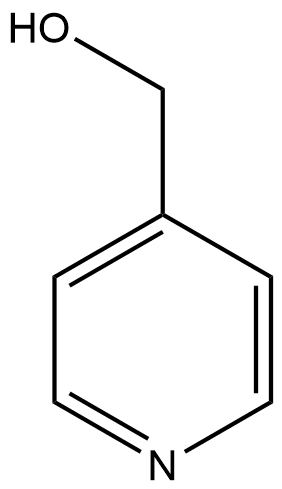
\includegraphics[scale=0.30]{figures/4HOMP.png}}
\quad
\subfigure[]{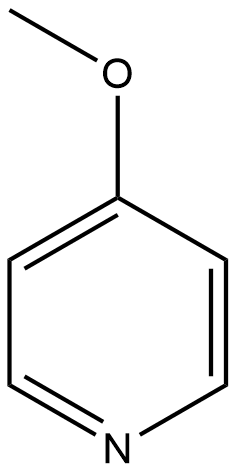
\includegraphics[scale=0.30]{figures/4-MOP.png}}
\caption{4-hydroxy-methyl-pyridine (a) and 4-methoxy-pyridine (b)}
\label{fig:4mophomp}
\end{figure}

The aim of this master thesis was the synthesis, spectral and structural characterization of new transition metal complexes using aforementioned pyridines with pseudohalides and transition metals.
Pseudohalides were chosen  as anionic ligands due to their similar properties to halides.  The central metal can bind to the end or middle atoms of these polyatomic ligands, making various combinations possible.\\

Mixing ligands and metal salts with varying ratios results in complexes with different coordination numbers (CN). Coordination numbers describe the number of donor atoms contained by ligands which are surrounding the central atom. 2, 4, 5 and 6 are common coordination numbers.\\

For the coordination number 2 only linear arrangements are  known and these complexes are often formed with the single positively charged ions \ce{Ag^+}, \ce{Cu^+} and \ce{Au^+}. \cite{riedel} \\

Tetrahedral and square-planar arrangements are possible for coordination number 4. Tetrahedral complexes are more common and are formed in all kinds of d-configurations whereas d$^8$-configuration (or 16-electron-complexes) prefer the square planar arrangement, i.e. \ce{Pt^{2+}} or \ce{Pd^{2+}}. \cite{riedel}   \\

Square-pyramidal and trigonal-bipyramidal structures are forms of the seldom appearing coordination number 5. They can be transformed into each other via Berry rotation \cite{berry} and are in equilibirium at a certain temperature.

CN 6 forms are octahedron (common), trigonal antiprism or trigonal prism (rare). The metal ions \ce{Cr^{3+}}, \ce{Co^{3+}} and  \ce{Pt^{3+}} favor the octahedral arrangement.\cite{riedel} \\

 
 The coordination numbers with their frequent arrangements are listed in figure \ref{fig:kz}.

\begin{figure}
\centering
\subfigure[CN2: linear]{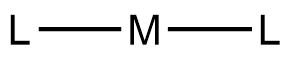
\includegraphics[width=0.30\linewidth]{figures/linear.png}}
\subfigure[CN4: square-planar]{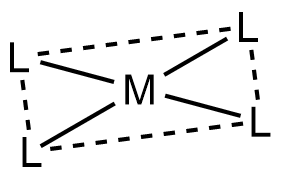
\includegraphics[width=0.30\linewidth]{figures/square-planar.png}}
\subfigure[CN4: tetrahedral]{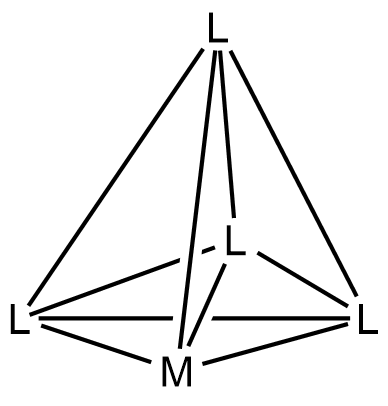
\includegraphics[width=0.30\linewidth]{figures/tetrahedral.png}}

\subfigure[CN5: square-pyramidal]{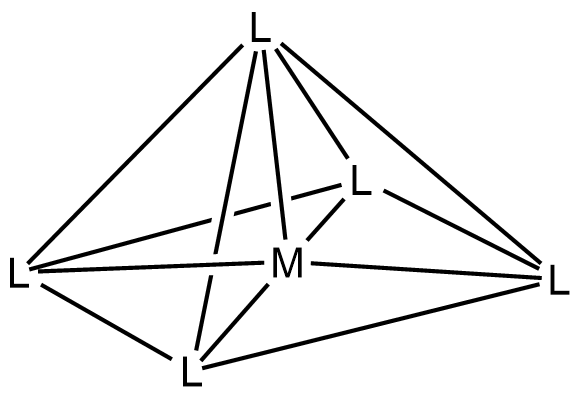
\includegraphics[width=0.30\linewidth]{figures/square-pyramidal.png}}
\subfigure[CN5: trigonal-bipyramidal]{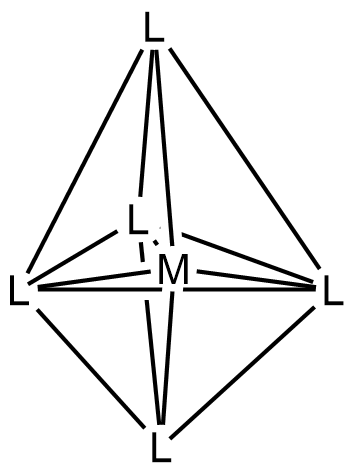
\includegraphics[width=0.30\linewidth]{figures/trigonal-bipyramidal.png}}
\subfigure[CN6: octahedral]{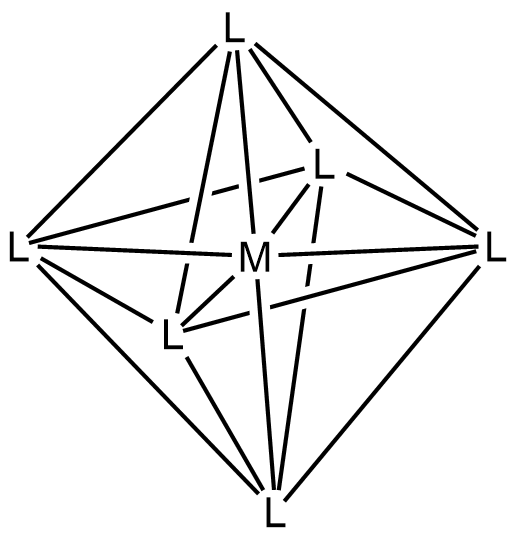
\includegraphics[width=0.30\linewidth]{figures/octahedral.png}}
\caption[Common structures of CNs]{Common structures of coordination numbers.}
\label{fig:kz}
\end{figure}
\part{Theory}
\chapter{Crystal structure analysis}
\label{ch:csa}
Chapter \ref{ch:csa} is adopted from the textbooks ``Kristallstrukturanalyse''  by W. Massa \cite{massa} and ``Einführung in die Röntgenfeinstrukturanalyse'' by H. Krischner \cite{krischner}. 
\section{Definitions}
A solid that contains atoms, ions or molecules which are arranged in a periodic pattern along the three dimensions of space is described as a crystal. For an arbitrary point picked in the crystal there are infinitely many points with identical surroundings. This is called periodicity. The crystal  can be considered infinitely extended in three dimensions. It can be seen as a lattice with a three dimensional array of points (lattice points). These points may not be considered as the ions or atoms in the crystal. If an atom is positioned on a lattice point, then the same atoms are at every lattice point in the crystal. \cite{massa}

 
\section{Bravais lattice}

7 crystal systems can be determined from a variation of the lattice parameters a, b, c and the angles $\alpha, \beta, \gamma$. Together with four types of centered cells (primitive (P), body-centered (I), face-centered (F) and base-centered (B)) 14 Bravais lattice types can be defined. \cite{bravais} For their determination the entire symmetry of the crystal should be contained in the smallest  unit of the cell. In table \ref{tab:cryssys} the crystal systems are listed.

\renewcommand{\arraystretch}{1.2}
\begin{table}[!htpb]
\centering
\captionabove{Crystal systems with their types of centered cell}
\begin{tabular}{|l|l|l|l|}
\hline
\textbf{Crystal system} & \textbf{Parameter} & \textbf{Angles} & \textbf{centered cell}\\
\hline
triclinic & $a\neq b\neq c$ & $\alpha\neq\beta\neq\gamma\neq 90^\circ$ & P\\
\hline
monoclinic & $a\neq b\neq c$ & $\alpha=\gamma=90^\circ \beta>90^\circ$ & P, B\\
\hline
orthorohmbic(cuboid) & $a\neq b\neq c$ & $\alpha=\beta=\gamma= 90^\circ$ & P, F, I, B \\
\hline
tetragonal & $a= b\neq c$ & $\alpha=\beta=\gamma= 90^\circ$ & P, I \\
\hline
hexagonal & $a= b\neq c$ & $\alpha=\beta= 90^\circ \gamma=120^\circ$ & P\\
\hline
trigonal (rhomboedric) & $a= b= c$ & $\alpha=\beta=\gamma\neq 90^\circ$ & P\\
\hline
cubic & $a= b = c$ & $\alpha=\beta=\gamma= 90^\circ$ & P, F, I\\ 
\hline
\end{tabular}
\label{tab:cryssys}
\end{table}

 \section{Diffraction}
 Electromagnetic waves can  interact with one-dimensional lattices. When monochromatic light (wavelength $\lambda$)  irradiates an optical grating (period d, which is the distance between two adjacent lines) and they are in the same order of magnitude, diffraction can occur. When a point of the lattice is struck with light, becoming a spherical wave of the same wavelength, it is called elastic scattering. The waves interfere with each other depending on the angle $\theta$ of observation and  the difference of the travelled path lengths by waves of the two adjacent points (optical retardation $\Delta$). Constructive interference can occur when $\Delta$ is an integer multiple of the wavelegth $\theta$. If all scattered waves in phase reinforce one another it leads to an observable diffracted beam. Destructive interferences between scattered waves can be observed if $\Delta$ is a half integer of $\theta$ and annulles them completely. In all other cases, where the values are between constructive and destructive interference, the lattice points can be grouped in pairs and be separated by one or more lattice points. These scattered waves are out of phase and cancel each other out. The intensity of the angles which meet the requirement of constructive interference exactly will be observed, the others will not.
 
 \begin{figure}[htpb!]
 \centering
 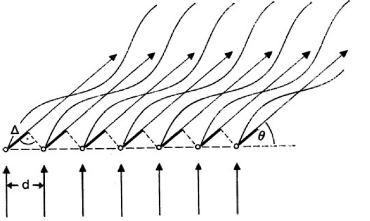
\includegraphics[width=0.7\textwidth]{figures/diffraction.png}
 \caption{Diffraction on a one dimensional lattice \cite{massa}}
 \label{fig:dif}
 \end{figure}
 
 \section{Bragg's Law}
In order to obtain diffraction, X-rays are  used since their wavelengths have the same order of magnitude as the inter-atomic distances in crystals, 1 \AA or 10$^{-10}$ m.  For three dimensional lattices, the one dimensional diffraction has to be adapted. The reflection of X-rays on lattice planes can be treated as diffraction. \cite{bragg} Only if constructive interference occurs (retardation is whole multiple of the wavelength) the conditions are fullfilled and Bragg's Law can  be derived (eq. \ref{eq:bragg}).  


\begin{figure}[htpb!]
\centering
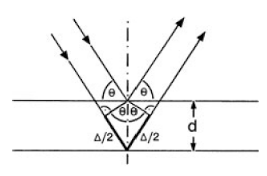
\includegraphics{figures/bragg.png}
\caption{Derivation of Bragg's Law \cite{massa}}
\label{fig:bragg}
\end{figure}


\begin{equation}
\begin{split}
2d sin(\theta) = n\lambda\\
 n=1,2,3,...
\label{eq:bragg}
\end{split}
\end{equation}



\section{hkl indices}
 All of the lattice planes contain lattice points and for each lattice plane there is a set of parallel and equidistant planes. Each lattice point lies on one plane. 
 For orientation of the planes there are the Miller Indices hkl. For the determination of the Miller indices for a set of planes, the plane nearest to the unit cell's origin (don't contain the origin)  is picked. This plane intersects the a-, b- and c-axes with the distances 1/h, 1/k and 1/l from the origin  measured in the axis lengths' units. 1/h, 1/k and 1/l can be represented as fractions, because they are rational numbers. The lattice planes can be denoted in parentheses (hkl) and hkl is used for the corresponding reflection. For parallel planes (to an axis) the intersection point lies at infinity and the Miller index is zero. For each set of lattice planes (hkl) with the characteristic distance d there is an unique angle $\theta$ for each diffraction order n at which reflection can be observed. (see Bragg's Law, eq. \ref{eq:bragg}). Each Miller index can be multiplied by n to determine the reflection at a lattice point.
 
 

 

 \section{Solution of Bragg's formula}
 To calculate the diffraction angle $\theta$ the distance of the corresponding lattice plane must be known. The distance d depends on the Miller indices (hkl) and the geometry of the lattice. The distance can be a square number (d$^2$) if different crystal systems are used. If Bragg's equation \ref{eq:bragg} is squared and d$^2$ is substituted, a quadratic Braggs' law is formed. It can be used to calculate $\theta$ from the Miller indices if the unit cell is known.
 
 
\section{Reciprocal lattice}
Each reflection is equivalent to a specific set of lattice planes. These sets are described by a vector d whose direction is vertical to the planes. Its length is equal to the distance between two adjoining planes. The endpoint of the corresponding vector d represents a lattice plane. For higher diffraction angles the length of d is shorter, which can be a drawback. Also hkl cannot be used to determine the direction of d. A new coordination system can help prevent these difficulties. It is spanned by the three base vectors a*, b* and c* and represents each plane (hkl) and each reflection hkl as the point ha*+ kb* + lc*. The reciprocal lattice is formed with the points of all possible coordinations of the indices, which are whole numbers. The original lattice is called the crystal lattice to distinguish the two.  The reciprocal base vectors are formed from the real base vectors in eq. \ref{eq:recv}, where each numerator is the vector product of two real base vectors and (abc) is the triple product equal to the volume of the real unit cell.
\begin{equation}
\begin{split}
a* =b x c/(abc)\\
b* = c x a/(abc)\\
c* = a x b/(abc)\\
\end{split}
\label{eq:recv}
\end{equation} 

 While in orthogonal crystal systems each reciprocal base vector is parallel to its counterpart, this is not true for systems with  oblique angles. Eq. \ref{eq:recv} suggests that every unit vector in reciprocal space is perpedicular to a plane in real space and vice versa. 

 \begin{figure}[htpb!]
\centering
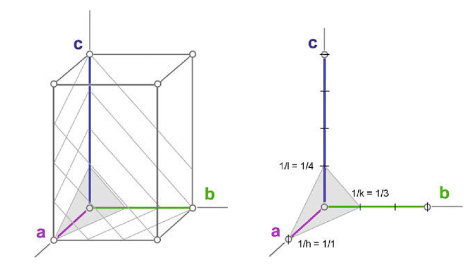
\includegraphics{figures/hkl-indices.png}
\caption{Definition of the hkl-indices through reciprocal axis intercept \cite{massa}}
\label{fig:hkl}
\end{figure}

\section{Intensity of diffracted X-rays}
With the knowledge of the geometry of the crystal lattice (the metric) the angles of all possible reflections can be determined. This is used in powder and single crystal measurements. The intensities of the reflections contain information about type and location of atoms in the unit cell. They can be measured absolute or relative. Absolute values are difficult to determine but relative values can be calculated and then be scaled to absolute values. How the atoms are arranged in the crystal can be calculated with these values. All factors should be known because they affect the intensities.

\section{Atomic scattering factor and temperature factor}
Up to now it was considered that X-ray scattering takes place at the points of the point lattice . In reality scattering occurs at the electrons or ions of atoms and crystals.  It was established that the radius of an electron shell has the same magnitude as the X-ray wavelength, but punctual scattering centers are not in the same range. Therefore  rays that are scattered at different positions in the electron shell have a phase difference. This leads to a weakening of the intensities which depends on the form of the shell and on the diffraction angle.  The scattering factors are scaled in a way that their values at an angle of zero are equal to the corresponding atomic number. \\
Atoms, depending on atom mass, chemical environment and temperature, oscillate about their equilibrium positions. X-ray beams consists of short radiation flashes that are approximately $10^{-18}$ s long. This is much shorter than the period of a thermal oscillation, lasting for $10^{-14}$ s. Because of this a specific atom can appear at slightly different locations during measurement. The result is a phase difference which increases with larger amplitudes (u) and smaller distances of the lattice planes, i. e. larger diffraction angles. This additional weakening of the scattering factors f is taken into account by multiplying the scattering factors with an e-function. At the beginning of a calculation the oscillations are assumed to be isotropic (see equation \ref{eq:os}). Substituting d in accordance with Bragg's Law eq. \ref{eq:bragg} and absorbing some constants in the Debye-Waller-factor B \cite{debye}\cite{waller} result in eq. \ref{eqdwfb}.

\begin{equation}
f' = f \cdot e^{-2\pi^2 \frac{u^2}{d^2}}
\label{eq:os}
\end{equation}



\begin{equation}
f' = f \cdot e^{-B\frac {sin^2 \theta}{\lambda^2}}
\label{eqdwfb}
\end{equation}

This affects the determination of lighter atoms, which have both low scattering factors and high amplitudes, due to their low mass. The crystals should be cooled when they are measured because of these reasons. When refining the crystal structure, oscillations are usually considered to be anisotropic with the exception of H-atoms. The displacement is now described by a tensor, represented by a symmetric 3x3 matrix with six independent factors,  U$_{11}$,  U$_{12}$,  U$_{13}$,  U$_{22}$,  U$_{23}$,  and U$_{33}$. By visualizing it as a thermal ellipsoid with three axes the corresponding atom can be found within the ellipsoid with 50\% probability. 


\begin{equation}
f'=f  \cdot e^{-2\pi^2(U_{11}h^2a^{*2}+U_{22}k^2b^*2+U_{33}l^2c^*2+2U_{23}klb^*c^* +2U_{13}hla^*c^*+2U_{12}hka^*b^*)}
\end{equation}


\section{Structure factor}

A reference point in the crystal is selected and all the other points whose surrounding are identical to that selected one  are determined in order to obtain the point lattice of the crystal. If a different reference point is picked, the same lattice is given, only shifted by the translation vector. This vector equals the difference of the spatial positioning between the first and second reference point. The same lattice applies to every atom in the unit cell, the chosen origin is the only difference. The crystal in fig. \ref{fig:pl} needs to be adjusted so that the lattice plane is at an appopriate angle $\theta$ with the X-ray beam. Then the waves of all type 1 atoms are in phase with each other.
\begin{figure}[htpb!]
\centering
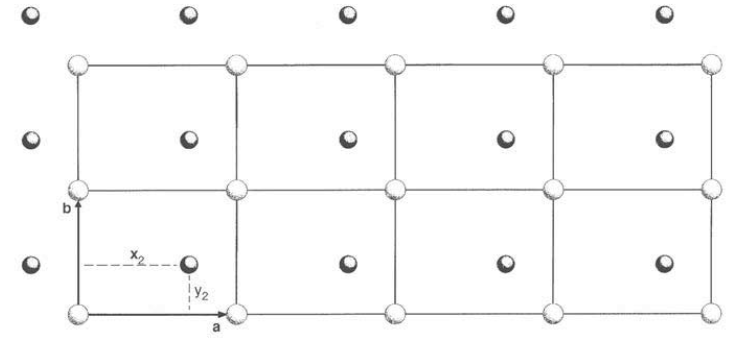
\includegraphics[width=1\textwidth]{figures/pointlattice.png}
\caption{2D- structure with two types of atoms \cite{massa} }
\label{fig:pl}
\end{figure}



 Waves generated by atoms of type 2 are also in phase with each other, because $\theta$ is not changed when the lattice is shifted . Since the lattice is translated a phase difference between the two diffracted rays exists. This depends on the relative position of the two atom types and on the selected lattice plane. Scattering factors are extended by a phase information, by multiplicating an exponential function with an imaginary argument: 




\begin{equation}
F_{hkl}(n) = f_n \cdot e^{i\phi_n}
\label{eq:hkl}
\end{equation}

For each atom of type n the phase angle $\phi$ expresses the phase difference. Euler's formula is applied to eq. \ref{eq:hkl} and gives an equivalent function with the sin und cos terms:

\begin{equation}
F_{hkl}(n)= f_n(cos(\phi_n)+i\cdot sin(\phi_n))
\end{equation}

In order to calculate $\phi_n$  the relative coordinates x$_n$, y$_n$, z$_n$ of atom n in the unit cell and the Miller indices of the lattice plane are taken into account: 

\begin{equation}
\phi_n = 2\pi(hx_n + ky_n + lz_n)
\end{equation}

For each reflection the diffracted waves of all atoms are added together with regard to their phase differences which leads to the final equation for the structure factor F$_{hkl}$ for a certain reflection hkl:

\begin{equation}
F_{hkl} = \sum_n f_n[cos(2\pi(hx_n + ky_n + lz_n)) + i\cdot sin(2\pi(hx_n + ky_n + lz_n))]
\end{equation}

For crystals belonging to a centro-symmetrical point group - with the origin of the crystal lattice being placed at a center of inversion - the calculation of the structure is reduced to:

\begin{equation}
F_{hkl} = \sum_n f_n cos(2\pi(hx_n + ky_n + lz_n))
\end{equation}

The structure factor cannot be measured directly because it is an imaginary quantity. Its relative intensity is determined and this is proportional to  the absolute value of F$_{hkl}^2$ . The phase angle $\phi$  cannot be obtained directly from the intensities, because it gets lost through the calculation -  this is called the phase problem. If the crystal has an inversion center, the phase problem can be simplified to determining the sign of F$_{hkl}$.

\section{Processing data}
For obtaining structure factors the raw data has to be processed after measurement. First the background signal is substracted and normalized if different periods are measured. The net intensity of each reflection is computed from the total intensity with this method. Intensities of reflections at different angles can be compared among each other when correction factors are applied. For powder diffractometry the multiplicity factor is relevant. This factor takes in consideration  that reflections of symmetry-equivalent lattice planes appear at the same angle in a powder diffractogram. The multiplicity factor normalizes the intensities since different lattice planes may have different numbers of symmetry equivalents. The value of the factor  ranges from 2 to 48 (triclinic to cubic system). The diffraction of X-rays is a reflection at certain planes in the crystal. The reflection angle $\theta$ is not important for the intensity of the fraction of the reflected beam, only if the electric component lies parallel to the plane. The intensity fraction is proportional to cos$^2$(2$\theta$) for radiation whose electric vector oscillates perpendicular to the plane. The polarization facor P makes it possible. Unpolarized X-rays leave the X-ray tube as a 1:1 mixture of rays with parallel and perpendicular electric field vectors to the reflection plane. Between these two extreme cases P is simply the average of the two:

\begin{equation}
P = \frac{(1 + cos^2(2\theta))}{2}
\end{equation}

A reflection is a curve with a certain breadth with its peak located at $\theta$ (Bragg's  angle). If a single crystal is rotated in the diffractometer the lattice planes stay in a reflection position for a period of time. It depends on the value of $\theta$ and is factored in the Lorentz factor L:

\begin{equation}
L = \frac{1}{sin(2\theta)}
\end{equation}

Lorentz and Polarization factor are summarized in the LP-correction:
\begin{equation}
LP=\frac{1+cos^2\theta}{2sin 2 \theta}
\end{equation}

The observed structure factor F$_0$ may be calculated as:
\begin{equation}
F_0=\sqrt {\frac{I}{LP}}
\end{equation}
 The absorption factor must also be taken into account. It affects the relative intensities of diffracted X-rays. While traveling through matter X-rays are weakened by elastic scattering, inelastic scattering and ionization. These absorption effects increase approximately with the fourth potency of the atomic number of the absorbing atom and with the third potency of the wavelength of the X-rays. All effects are summarized in the linear absorption coefficient ($\mu$) and the intensity can be calculated with eq.\ref{eq:lac} (s is the travelled distance of the X-ray beam):

\begin{equation}
I = I_0\cdot exp(-\mu\cdot s)\\
\label{eq:lac}
\end{equation}

From tabulated values for components of the crystal, their mass fraction in the crystal and the density of the crystal $\mu$ can be obtained. Different methods for absorption corrections (for higher $\mu$ values) have been developed, e.g. numeric absorption correction, empiric absorption correction and the DIFABS method \cite{wal83}.

\section{Laue class}
For determination of the space group the Laue class must be derived. Each reflection is a point in the reciprocal lattice. Assigning the intensity to each reflection of its point in reciprocal space yields the intensity-weighted reciprocal lattice. Its point group is the Laue class of the crystal. The Laue class contains a center of inversion (even if the crystal has none) which is the only difference between the space group and the Laue class. The two reflections hkl and h-k-l refer to the same set of lattice planes except they are only irradiated from opposing sites. All Laue groups include two or more point groups and each point group contains several space groups. \\
For reducing the number of possible space groups systematic extinctions can be found. They are absences of reflections whose indices satisfy certain conditions. They show that glide planes, screw axes or centered unit cells can be present in the cell. For crystal systems of high symmetry the space group can be hardly determined. For these cases informaton about physical properties, Patterson symmetry and structure-chemical plausibility is important.  


\section{Direct methods}
These methods attempt to obtain phases of the structure factors directly from measured intensities through mathematical relationships. The original works for these methods  \cite{harker48} found that the presence of symmetry elements gives rise to relations between structure amplitudes and certain pairs of reflection. The assumption that the electron density consists of identical and well-resolved peaks result in the equation \ref{eq:dm} \cite{sayre}:
\begin{equation}
E_{hkl} = C \sum_{h^{'}k^{'}l^{'}}E_{h^{'} k^{'} l^{'}} \cdot E_{h-h^{'} k-k^{'} l-l^{'}}
\label{eq:dm}
\end{equation}

To obtain the normalized structure factor E$_{hkl}$ F$_{hkl}$ is divided by its expectation value. This value can be calculated from the Wilson statistic. \cite{wilson}  Eq.\ref{eq:dm} applies to structures containing just one type of atom but in practice it can also be used for structures with atoms with similar atomic number; e.g. C, N, O, H. Therefore it can be applied for classes of structures that are difficult to solve via Patterson methods.



\section{Patterson method}
For crystals containing only a few heavy elements (which is the case for most metal-organic compounds) the Patterson method can be of use, as it  solves the phase problem.
In the Patterson function P$_{uvw}$, the coefficients are the directly measured F$_0^2$ values. To distinguish the patterson synthesis from a normal F$_0$ Fourier synthesis, the coordinates in Patterson space have the coordinates u, v and w. These 
coordinates are not directly related to atomic coordinates x, y, z, altough they refer to the same axes and unit cell. 
The Patterson function is defined as:
\begin{equation}
P_{uvw}= \frac{1}{V} \sum \limits _{hkl}\left|F_{hkl}\right|^{2} cos(2\pi(hu + kv + lw))
\end{equation}

The Patterson function only include the information  from the intensities, the interatomic vectors, because no phase information is contained in the F$_0^2$ values.  \cite{patterson}\\

Maxima in the function P represent distance vectors between atoms in the unit cell. P is always centrosymmetric since two distance vectors of the same length and opposite direction are associated with each pair of atoms. The intensity of a Patterson peak is simply the product of the atomic number of the two atoms involved. If a crystal contains a few heavy metal atoms, they can easily be identfied by the high intensities of the corresponding peaks. 



\chapter{Pseudohalide complexes}
\section{Chemical properties}
Pseudohalogenes are polyatomic molecules posessing properties similar to halogenes and are therefore among the group of pseudoelements. These chemical properties are reactivity, charge and binding behavior. They can be used as substitutions for halogenes in all kinds of chemical  compounds. Pseudohalides, the ionic form of pseudohalogenes, are used as ligands in coordination complexes. Cyanide, cyanate, thiocyanate, azides and rhodanides are well known pseudohalides. The chemical properties and their behavior are identical to halide ions. The internal double or triple bonds that are often present do not affect their chemical behavior. They form strong acids (HX) and  react with metals to form compounds like MX. \cite{holub}


\section{Azide complexes}

Azide (\ce{N_3^-}) is the salt of hydrazoic acid. \ce{HN_3} is a weak base (pk$_a$ of 4.75) and is highly explosive in its waterfree form.
Hydrazoic acid and azides are highly toxic and should be handled with care. The linear molecule N$_3^-$ has three possible resonance structures: \\
\ce{ ^{-}N = N^{+}= N^{-} <=> N# N^+ - N^{2-} <=> ^{2-}N - N^+ # N}\\
Azide can be organised in two types: inorganic  (e.g. NaN$_3$) and organic azides (e.g. TosN$_3$). \cite{holub}
 Furthermore, azides can be subdivided in more types according to their bonding character \cite{mueller}: Ionic azides, molecular azides and coordinative azides.\\
Azides are used for technical applications such as explosives (\ce{Pb(N3)2}), airbags or pharmacy. Fig. \ref{fig:az} depicts bridging modes of azides. 
\begin{figure}[htpb!]
\centering
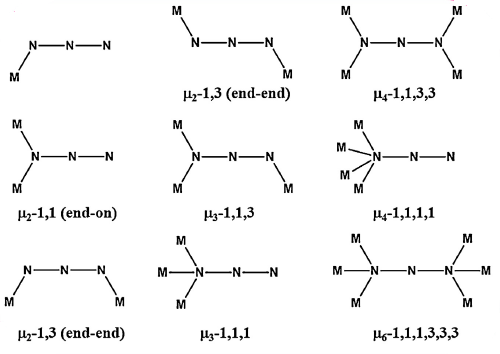
\includegraphics[scale=1]{figures/azidescheme.png}
\caption{Structures of published azide complexes \cite{han2015}}
\label{fig:az}
\end{figure}

\section{Rhodanide and cyanate complexes}
Thiocyanate (alternate name rhodanide) is the conjugate base of thiocyanic acid. Common derivatives are KSCN and NaSCN. Rhodanite is an analogue of the cyanate ion (\ce{OCN^-}). The name rhodanide means rose in greek  and comes from the red colour of its iron complexes. If the metal or the organic group is attached to the S (\ce{R-S-C#N}) the compound is called thiocyanate and if it is bonded to the N-atom (\ce{R-N=C=S}) its name is isothiocyanate. \cite{guy1977} Two equivalent resonance structures exist:\\
\ce{S=C=N^- <=> ^-S-C#N} \\
As a result thiocyanate is an ambidentate ligand, meaning that both ends (S or N) can act nucleophilic. In fig. \ref{fig:ocnscn} I-VI are listed the known bonding types. Hard acids form N-bonded isothiocyanate complexes and soft acids form S-bonded thiocyanate complexes.\cite{holub}  \\
\begin{figure}[htpb!]
\centering
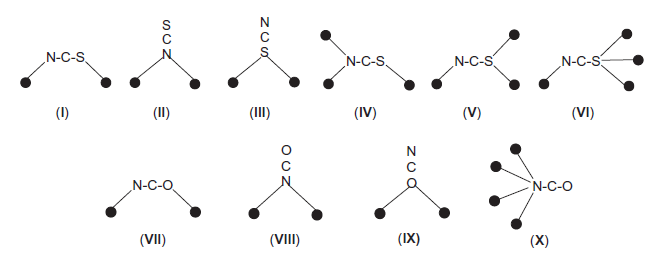
\includegraphics[width=1\textwidth]{figures/schemeocnscn.png}
\caption{Some thiocyanate and cyanate coordination bridging modes. Points represent metallatoms. \cite{fam}}
\label{fig:ocnscn}
\end{figure}

Cyanate's chemical structure is [OCN]$^-$ or [NCO]$^-$. It has similar properties to thiocyanate. In figure \ref{fig:ocnscn} (VII) to (X) the different bonding types are shown.  If the metal or the organic group is attached to the O (\ce{R-O-C#N}) the compound is called cyanate and if it is bonded to the N-atom (\ce{R-N=C=O}) its name is isocyanate. \cite{holub}


\section{Dicyanamide complexes}




The molecular formula for dicyanamide is \ce{C_2N_3^-}. It is composed of two cyanide groups that are bound to a central nitrogen anion. It can be used as a counterion in organic and inorganic salts and as reactant for the synthesis of covalent organic structures.
Another use would be the synthesis of pseudohalide complexes. The metal  can bind on the middle and end nitrogen atoms of the dicyanamide. Therefore there are a lot of combinations how the metals can be bound to a single dicyanamide. \cite{holub} In fig. \ref{fig:syndca} there are examples of structures of published dca complexes. Fig. \ref{fig:nosyndca} contains structures which have not been synthesized yet but are also possible. 

\begin{figure}[h!]
\centering
\subfigure[0-1-0]{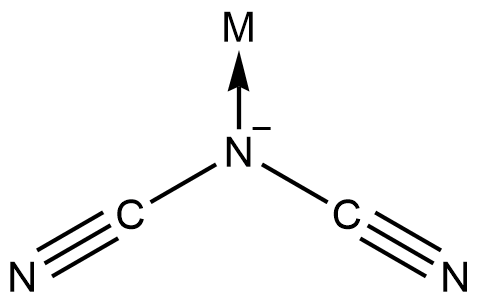
\includegraphics[scale=0.35]{figures/dca0-1-0.png}}
\quad
\subfigure[1-0-0]{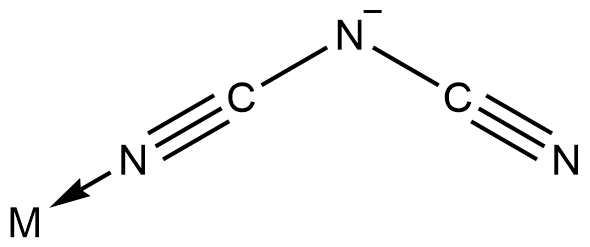
\includegraphics[scale=0.35]{figures/dca1-0-0.png}}
\subfigure[1-0-1]{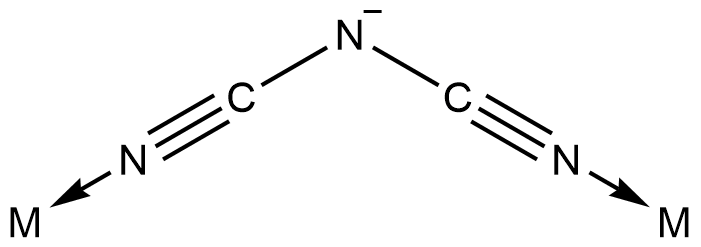
\includegraphics[scale=0.35]{figures/dca1-0-1.png}}
\quad
\subfigure[1-1-0]{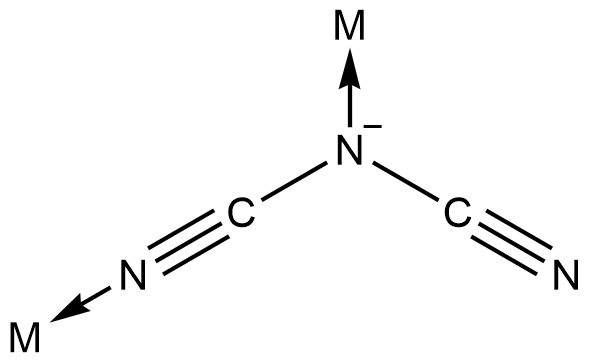
\includegraphics[scale=0.35]{figures/dca1-1-0.png}}
\subfigure[1-1-1]{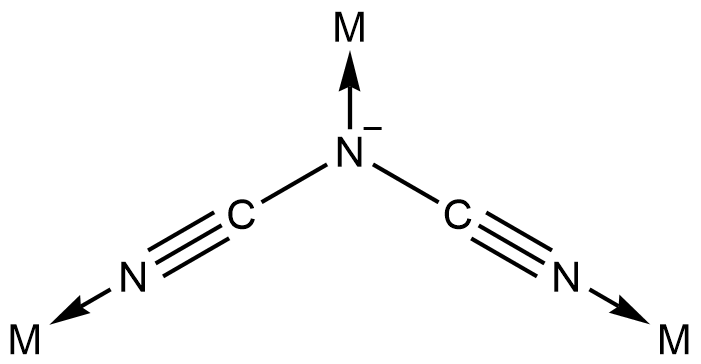
\includegraphics[scale=0.35]{figures/dca1-1-1.png}}
\quad
\subfigure[2-0-0]{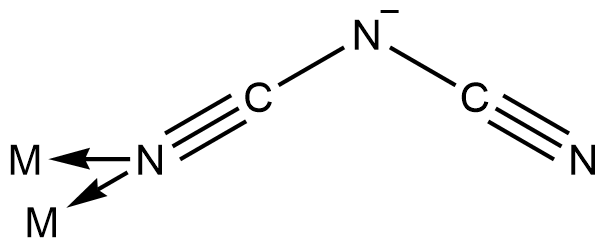
\includegraphics[scale=0.35]{figures/dca2-0-0.png}}
\subfigure[2-0-1]{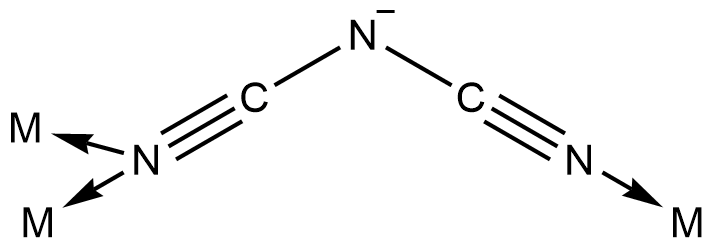
\includegraphics[scale=0.35]{figures/dca2-0-1.png}}
\quad
\subfigure[2-0-2]{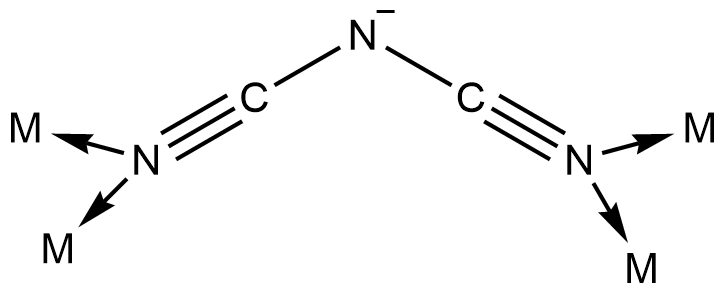
\includegraphics[scale=0.35]{figures/dca2-0-2.png}}

\caption{Structures of published dca complexes in the CCDC \cite{ccdc}}
\label{fig:syndca}
\end{figure}


\begin{figure}[h!]
\centering
\subfigure[2-1-0]{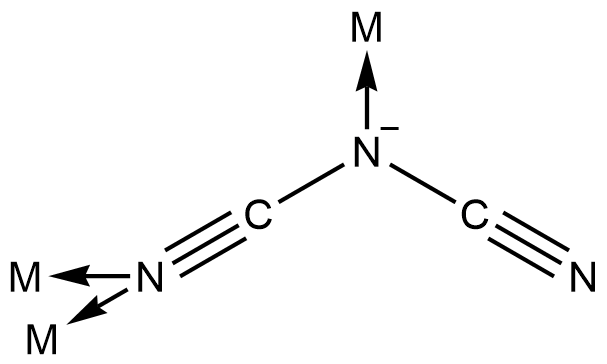
\includegraphics[scale=0.35]{figures/dca2-1-0.png}}
\quad
\subfigure[3-0-0]{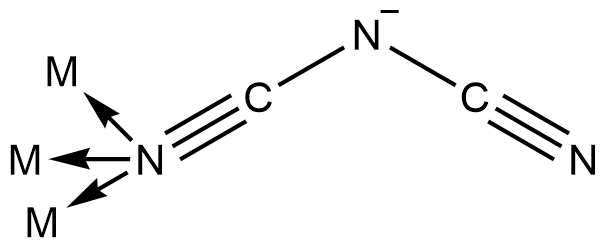
\includegraphics[scale=0.35]{figures/dca3-0-0.png}}
\subfigure[3-0-2]{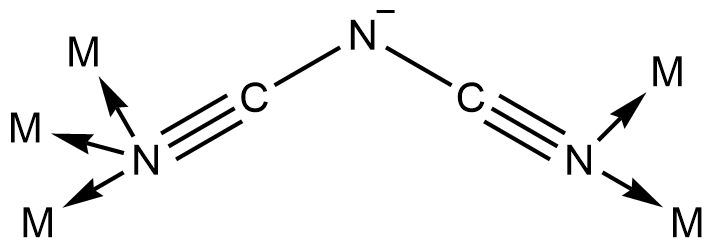
\includegraphics[scale=0.35]{figures/dca3-0-2.png}}
\quad
\subfigure[3-0-3]{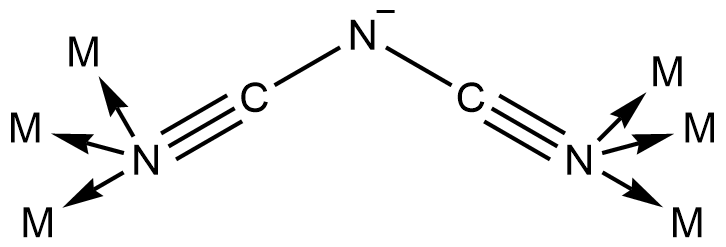
\includegraphics[scale=0.35]{figures/dca3-0-3.png}}
\subfigure[4-0-0]{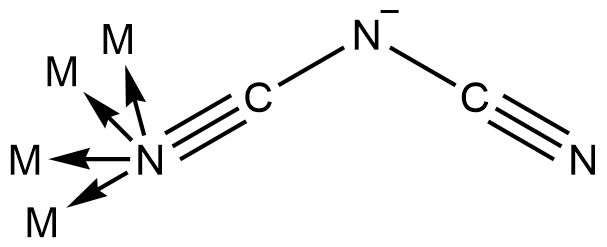
\includegraphics[scale=0.35]{figures/dca4-0-0.png}}


\caption{Structures of possible dca complexes which are not  published yet}
\label{fig:nosyndca}
\end{figure}









\chapter{Pyridines}
Pyridines are described as six- membered heterocycles, which include a single N-atom in the ring. They are aromatic compounds and their  6 $\pi$-electrons are delocalized over the entire ring. All atoms in the ring are sp$^2$ hybridized. The N-atom has a lone pair which does not contribute to the aromatic system and has influence on the chemical properties of the pyridine.
It's hydrophilic and hydrophobic character makes it miscible with water and organic solvents. \cite{joule}

Pyridines can be involved in  protonation, alkylation, acylation and N-oxidation as  tertiary amines and nucleophilic substitution as aromatic compounds.

The compound itself is a weak ligand for forming complexes with transition metal ions, but its acid derivates can form strong complexes.

With a pk$_a$ of approximately 5 pyridines are weak bases and therefore the formation of salts is favored.
The electronegative nitrogen in the ring makes the pyridine an electron deficient molecule. Therefore it is more improbable for the compound to partake in electrophilic reactions unlike other benzene derivatives. Nucleophilic substitution and metalation, however, occur more often with pyridines and are conducted using strong organometallic bases. \cite{joule1}

\begin{figure}[htpb!]
\centering
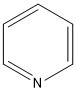
\includegraphics{figures/pyridine.jpg}
\caption{Chemical structure of pyridine}
\label{fig:py}
\end{figure}

\section{4-hydroxy-methyl-pyridine complexes}
\label{ch:4HOMP}
\renewcommand{\arraystretch}{1.3}
\begin{longtable}{|p{1\textwidth}|}

 \captionabove{List of in the CCDC published 4-hydroxy-methyl-pyridine complexes \cite{ccdc}}
 \label{tab:pubpy}\\
 \hline
 trans-[PtCl$_2$NH$_3$(4-(hydroxymethyl)-pyridine)] \cite{RamosLima20033379}\\
 \hline
 [Mn$_6$O$_2$(O$_2$CPh)$_10$(4-hydroxymethylpyridine)$_3$(MeCN)] \cite{Stamatatos20061737}\\
 \hline
 catena-(($\mu_2$-pyridine-2,6-dicarboxylato)-($\mu_2$-4-(hydroxymethyl)pyridine)-copper(II) \cite{Ucar2009}\\
 \hline
 Diaqua-(pyridine-2,6-dicarboxylato)-(4-hydroxymethyl)pyridine)-nickel(II) monohydrate \cite{Ucar2009}\\
 \hline
 [Ag(4-hydroxymethylpyridine)$_2$]NO$_3$ \cite{KalinowskaLis2014394}\\
 \hline
 trans-[PtCl$_2$(NH$_2$CH(CH$_3$)$_2$(4-py-MeOH))] \cite{KalinowskaLis20081328}\\
 \hline
 trans-[PtCl$_4$(NH$_3$)(4-py-MeOH)] \cite{KalinowskaLis20081328}\\
 \hline
 [Cu(4-pyridylmethanol)$_4$Cl]Cl \cite{monc2004}\\
 \hline
bis(Glycinato-N,O)-bis(4-hydroxymethylpyridine-N)-nickel \cite{zhao2010}\\
\hline
chloro-(2-(isobutylimino)methylphenolato)-((pyridin-4-yl)(methanol))-platinum dichloromethane solvate \cite{rahman2015}\\
\hline
bis(Niflumato-O)-bis(4-pyridylmethanol-N)-copper(II) methanol solvate \cite{maroszova2011}\\
\hline
Aqua-bis(2-chlorobenzoato-O)-bis(4-pyridylmethanol-N)-copper(II) \cite{maroszova2011}\\
\hline
tetrakis($\mu_2$-(2,6-Diisopropylphenyl)phosphato)-tetrakis(4-(hydroxymethylpyridine)-tetra-zinc \cite{murugavel2006}\\
\hline
bis($\mu_4$-Oxo)-tetrakis($\mu_3$-benzoato)-hexakis($\mu_2$-benzoato)-(acetonitrile)-tris(4-hydroxymethylpyridine)-tetra-manganese(II)-di-manganese(III) acetonitrile solvate \cite{stamatatos2006}\\
\hline
tetrakis($\mu_2$-acetato)-bis(4-pyridinemethanol)-di-rhodium)  \cite{ye2011}\\
\hline
(Cyclobutane-1,1-dicarboxylato)-(bis((pyridine-4-yl)methanol)-platinum \cite{escribano2013}\\
\hline
bis($\mu_2$-cyclohexane-1,2-dicarboxylic acid)-(tetrakis((pyridin-4-yl)methanol)-di-platinum dihydrate \cite{escribano2013}\\
\hline
catena-[tris($\mu_2$-Azido-N$^1$,N$^1$)-($\mu_2$-Azido-N$^1$,N$^3$)-tetrakis(4-hydroxymethylpyridine)-di-cadmium(II)] \cite{goher2008}\\
\hline
bis((pyridin-4-yl)methanol)-(trifluormethanesulfonato)-silver \cite{deBoer2014}\\
\hline
bis(pyridin-4-yl)methanol)-silver perchlorate \cite{deBoer2014}\\
\hline
bis((pyridin-4-yl)methanol)-silver tetrafluoroborate acetonitrile solvate \cite{deBoer2014}\\
\hline
tetrakis((pyridin-4-yl)methanol)-bis(thiocyanato)-nickel \cite{werner2015}\\
\hline
bis(ethanol)-bis((pyridin-4-yl)methanol)-bis(thiocyanato)-nickel \cite{werner2015}\\
\hline
diaqua-bis((pyridin-4-yl)methanol)-bis(thiocyanato)-nickel \cite{werner2015}\\
\hline
catena-[($\mu$-pyridin-4-ylmethanol)-($\mu$-thiocyanato)-(pyridin-4-ylmethanol)-(isothiocyanato-nickel] \cite{werner2015}\\
\hline
Aqua-bis(4-clofibriato-O)-bis(4-pyridylmethanol-N)-copper(II) dihydrate \cite{moncol2004}\\
\hline
tris(Tetraethylammonium)-tris($\mu_2$-4-pyridinemethanolato)-bis(tricarbonyl-tungsten(0)) acetonitrito solvate \cite{klausmeyer2004}\\
\hline
chloro-tetrakis(pyrid-4-ylmethanol-N)-copper(II) chloride \cite{moncol2004}\\
\hline
trans-dichloro-isopropylamine-(4-(hydroxymethyl)pyridine-N)-platinum(II) \cite{ramoslima2006}\\
\hline
bis(pyridin-4-yl-N)methanol)-silver nitrate \cite{deBoer2014}\\
\hline
catena-($\mu_2$-Pyridin-4-ylmethanol)-($\mu_2$-thiocyanato-N,S)-isothiocyanato-(4-(hydroxymethylpyridine)-cadmium) \cite{werneracta}\\
\hline
Tetrakis($\mu_2$-Acetato-O, O')-bis(4-pyridylmethanol-N)-di-copper(II) \cite{hoang1993}\\
\hline
Aqua-bis(-bromobenzoato-$\kappa$O)-bis(4-pyridylmethanol-$\kappa$N)-copper(II) \cite{moncol2008}\\
\hline
catena-[($\mu$-adipato)-bis((pyridin-4-yl)methanol)-aqua-copper] \cite{chechova2015}\\
\hline
\end{longtable}
 
 \section{4-methoxy-pyridine complexes}
 \label{ch:4MOP}
 \begin{longtable}{|p{1\textwidth}|}
 
 \captionabove{List of in the CCDC published 4-methoxy-pyridine complexes \cite{ccdc}}
 \label{tab:pubmepy}\\
 \hline
 bis(acetonitrite)-tetrakis(4-methoxypyridine)-di-silver dihexafluorophosphate \cite{wong2015}\\
\hline
 bis($\mu_2$-iodo)-bis(4-methoxypyridine)hexamethyl-di-platinum \cite{gosh2015}\\
 \hline
 diaqua-(chelidamato)-(4-methoxypyridine)-nickel(II) dihydrate \cite{ucar2015}\\
 \hline
 diaqua-(chelidamato)-(4-methoxypyridine)-cobalt(II) dihydrate \cite{ucar2015}\\
 \hline
 tetrakis(4-methoxypyridine)-dioxo-rhenium(V) hexafluorophosphate \cite{canlier2010}\\
 \hline
 (4-Methoxypyridine)-(pyridine-2,6-dicarboxylato-N,O,O')-copper(II) \cite{perry2004}\\
 \hline
 bis(cyano)-(tetrakis(4-methoxypyridine))-ruthenium \cite{pieslinger2013}\\
 \hline
bis($\mu_2$-cyano)-dichloro-octapyridyl-tetrakis(4-methoxypyridine)-tri-ruthenium bis(hexafluorophosphate) \cite{pieslinger2013}\\
\hline
chloro-(p-methoxypyridine)-(2-(2-pyridyl)phenyl)-platinum(II) chloroform \cite{godbert2007}\\
\hline 
(benzo(h)quinolin-10-yl)-chloro-(p-methoxypyridine)-platinum(II) \cite{godbert2007}\\
\hline
bis(acetato)-aqua-bis(4-methoxypyridine)-cadmium \cite{saxena2015}\\
\hline
catena-(bis-$\mu_4$-Benzene-1,3-dicarboxylato)-bis(4-methoxypyridine)-di-zinc(II) methanol  ciathrate \cite{abourahma2003}\\
\hline
catena-(bis$\mu_4$-Benzene-1,3-dicarboxylato)-bis(4-methoxypyridine)-di-zinc(II) benzene ciathrate) \cite{abourahma2003}\\
\hline
tricarbonyl-(4-methoxypyridine)-pyridine-2-carboxylato)-rhenium \cite{hayes2015}\\
\hline
cis-1,2-Dichlorovinyl(4-methoxypyridine)-cobaloxime chloroform solvate \cite{follet2007}\\
\hline
Tetracarbonyl-(4-methoxypyridine)-(triphenylphosphine)-tungsten \cite{carlton2013}\\
\hline
catena-($\mu_3$-1,2-Benzoisothiazole-3-thionato-1,1-dioxide-S,S,S)-($\mu_2$-1,2-benzoisothiazole-3-thionato-1,1-dioxide-S,S)-bis(4methoxypyridine)-di-silver(II) \cite{dennehy2010}\\
\hline
($\eta^2, \eta^2$-Cyclo-octa-1,5-diene)-(4-methoxypyridine)-tricyclohexylphosphine-iridium hexafluorophospate \cite{mantilli2012}\\
\hline
bis(4-methoxypyridine)(propane-1,3-diylbis(diphenylphosphine)-platinum bi(fluoromethanesulfonate) monohydrate \cite{weilandt2012}\\
\hline
bis(4-methoxypyridine)(propane-1,3-diylbis(diphenylphosphine)-palladium bis(fluoromethanesulfonate) monohydrate \cite{weilandt2012}\\
\hline
Chloro-(dihydrogen dimethyl glyoximato)-(4-methoxypyridine)-(dimethyl glyoximato)-cobalt diethyl ether solvate \cite{wakerley2014}\\
\hline
bis(4-methoxypyridine)-(2,2'.6',2''.6'',2'''-quaterpyridine)-ruthenium diperchlorate monohydrate \cite{liu2014}\\
\hline
(3,5-di-t-butylcatexholato)-(3,5-di-t-butyl-o-semiquinonanto)-bis-(4methoxypyridine)-cobalt(II) \cite{schmidt2010}\\
\hline

 \end{longtable} 
 
 
 \section{Comparison between 4-HOMepy and 4-MeOpy}
 4-Hydroxymethylpyridine (4-HOMP) is an alcohol. By removing the H-atom of the alcohol group, metal atoms can bind to the oxygen of the formed alkoxid group. Due to this, 4-HOMP can be used as a bridging ligand. \\
However, this is not possible for 4-methoxypyridine (4-MOP). Hydrogen abstraction from its ether moiety is too unlikely. Thus, it can not from an additional bond, rendering 4-MOP unable to be used as a bridging ligand.\\
With a melting point of 52-56$^\circ$C and a boiling point of 107-110$^\circ$C 4-HOMP is a solid at room temperature and should be stored in the fridge. 4-Methoxypyridine has the same boiling point but a melting point at 4$^\circ$C and is therefore a liquid at 20$^\circ$C. \cite{sigma} \cite{sigma2}

\part{Experimental}
\chapter{Preparation and technical data}
\section{General overview}
The chemicals used in the synthesis of the complexes were provided by Merck. No further purification was necessary. Destilled water was used as solvent for all reactions. All chemicals were handled with care and only small doses were used. For the reactions 100 mL flasks with screw caps were used. The solutions were  heated in waterbaths standing on heating plates. For a  slow cooling to room temperature the heating plates were shut off and the flasks were left in the waterbaths until 20$^\circ$C were reached. If no crystals were obtained the screw caps were removed, so the water could slowly evaporate. The crystalls were obtained using filtration under reduced pressure.\\
The IR spectra of the dca complexes were compared with the IR-spectrum of sodium dicyanamide in the attachment p. \pageref{fig:dca-ir}, the other complexes (azide, cyanate and rhodanide) were compared with literature. \cite{kazuo} 
\section{Used devices and programs}
For single crystal X-ray measurement the following devices were used:
A Bruker and APEX II CCD diffractometer (MoK$\alpha$ radiation $\lambda$ = 0.71073 \AA) with $\omega$-scan mode and
graphite-monochromator at 100K. Data was collected and processed using APEX and SAINT \cite{apex} software packages. All data was corrected, for absorption  Laue symmetry requirements were applied. \cite{laue}
The SHELXTL/PC program package \cite{shelxtl} was applied for  structure solution (direct methods) and structure refinement (least squares). PLATON \cite{platon} (a program for automated
calculation of derived geometrical data) was used for supporting the structure solution process.
Additionally a Bruker-AXS SMART APEX CCD diffractometer at 100K with Mo-radiation ($\lambda$ = 0.7107 \AA) and
graphite monochromator was used.
Data was collected by Assoc.Prof. Dipl.-Ing. Dr.techn. Roland Fischer and structure refinement was done by Ao. Univ.-Prof. Dr. Franz A. Mautner.
\\For IR-analysis an Alpha-P spectrometer by Bruker was provided. It was used to characterize specific bands from pyridines and pseudohalides. The spectra were measured in the range of  400 cm$^{-1}$ to 4000 cm$^{-1}$ with the program Opus. \cite{opus}
\\The UV-VIS-measurements were conducted using a Lambda 950 UV/ VIS/ NIR spectrometer by Perkin Elmer. Measurement of the spectra ranged from 200 to 2500 nm. The program for processing and data collection was UVWINLab software. \cite{uvwin}


\chapter{4-methoxy-pyridine complexes}
\section{\ce{[Co(N_3)_2(4-methoxypyridine)_4]}}
\label{CoA4MOP}
\subsection{Synthesis}
0.28 g \ce{CoSO_4 * 7 H_2O} (1 mmol), 0.13 g sodium azide (2 mmol) and 0.44 g 4-methoxy-pyridine (4 mmol) were dissolved in 20 mL distilled water. The solution was warmed up to $60^\circ$C  and stirred for 2 hours and 30 minutes. The clear pink solution was stirred again after filtration for 1 hour at the same temperature and then cooled down to 20$^\circ$C. Pink crystals were obtained after one day.\\ Anal. Calculated for \ce{C_{24}H_{28}CoN_{10}O_{4}} (579.49 g/mol) : 49.74\% C; 4.87\% H; 24.17\% N;\\
Found: 49.45 \% C; 4.84\% H; 24.32 \% N;\\
IR (ATR, cm$^{-1}$): 2037 (m), 1603 (s), 1564 (m), 1508(m), 1495 (m),1454 (m), 1430 (m), 1291 (s), 1207 (s), 1057 (w), 1020 (s), 805 (s), 642 (w), 539 (s), 457 (w)

\begin{figure}[h!]
\centering
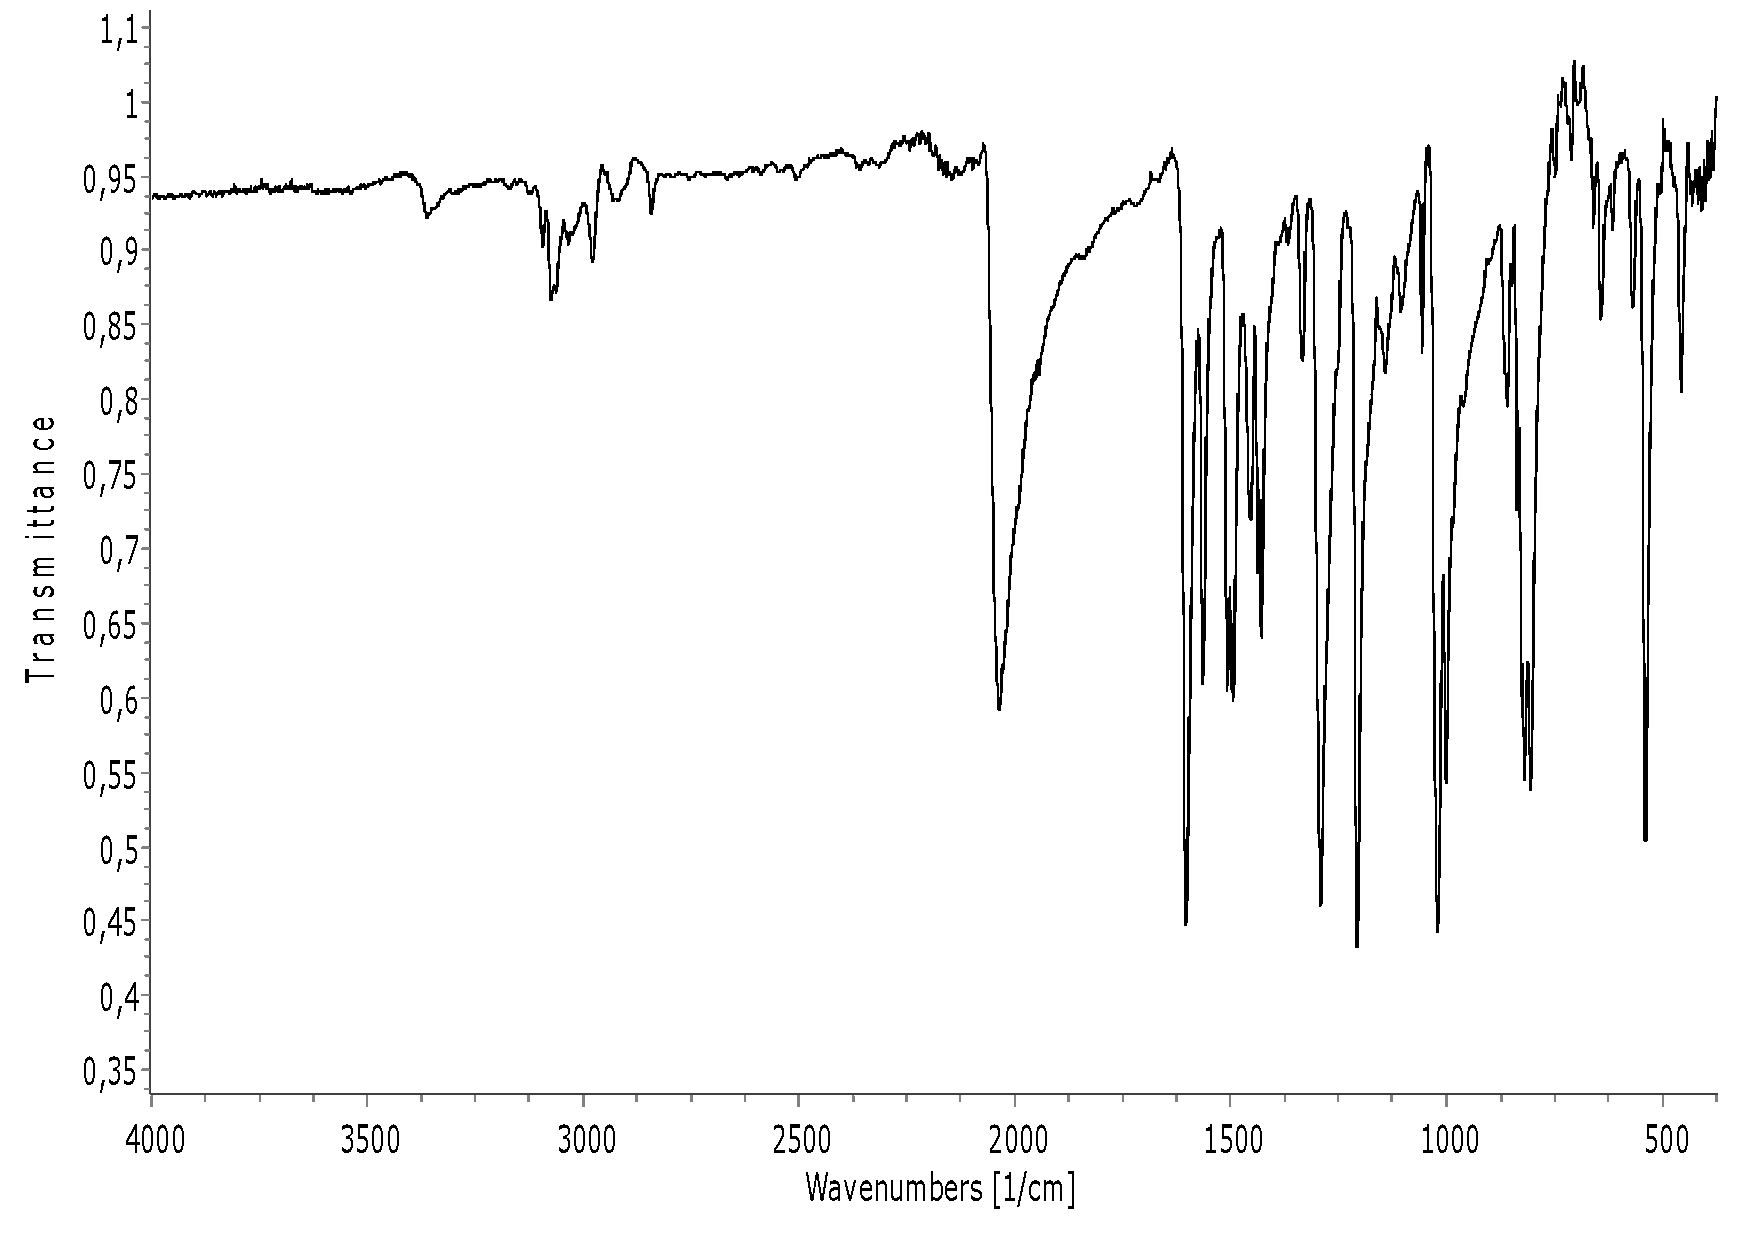
\includegraphics[scale=0.5, width=0.95\textwidth]{figures/CoA4MOP-IR.pdf}
\caption{IR spectrum of \ce{[Co(N_3)_2(4-MeOpy)_4]}}
\end{figure}

\newpage
\subsection{Structural characterization}

Fig. \ref{fig:CoA4MOP_pv} and fig. \ref{fig:CoA4MOP_packv} show a perspective view and a packing view of  \ce{[Co(N_3)_2(4-MeOpy)_4]}. Selected bond parameters are summarized in table \ref{batlb:CoA4MOP}. The complex consists of two crystallographically independent mononuclear and neutral Co(II) complexes. Each Co(II) is six-coordinated by N atoms of two terminal azido groups, as well as N-donor atoms of four neutral 4-methoxy-pyridine molecules. The \ce{CoN_6} chromophores may be described as slighly distorted octahedra with trans-arrangement of the azido ligands. The Co-N bond lengths are in the range of 2.085(3) to 2.202(3) \AA , and the transoid N-Co-N bond angles within the \ce{CoN_6} octahedra vary from 171.61(11) to 177.35(12)$^\circ$. The bond parameters of the terminal azido groups are: Co-N-N: from 125.6(2) to 129.1(3)$^\circ$, N-N-N: from 178.3(4) to 179.3(4)$^\circ$, N(x1)-N(x2): from 1.192(4) to 1.199(4) \AA, N(x2)-N(x3): from 1.165(5) to 1.175(4) \AA.The shortest metal-metal separation is 8.2523(8) \AA. 


\renewcommand{\arraystretch}{1.5}
\begin{table}
\captionabove{Selected bond lengths (\AA) and angles ($^\circ$) for  \ce{[Co(N_3)_2(4-MeOpy)_4]}}
\centering
\begin{tabular}{|l|l|l|l|}
\hline
Co(1)-N(11) & 2.103(3) & Co(2)-N(31) & 2.116(3)\\
\hline
Co(1)-N(21) & 2.125(3) & Co(2)-N(41) & 2.085(3)\\
\hline
Co(1)-N(1) & 2.170(3) & Co(2)-N(5) & 2.173(3)\\
\hline
Co(1)-N(2) & 2.184(3) & Co(2)-N(6) & 2.181(3)\\
\hline
Co(1)-N(3) & 2.189(3) & Co(2)-N(7) & 2.202(3)\\
\hline
Co(1)-N(4) & 2.161(3) & Co(2)-N(8) & 2.188(3)\\
\hline
N(11)-N(12) & 1.196(4) & N(12)-N(13) & 1.167(4)\\
\hline
N(21)-N(22) & 1.194(4) & N(22)-N(23) & 1.175(4)\\
\hline
N(31)-N(32) & 1.192(4) & N(32)-N(33) & 1.167(5)\\
\hline
N(41)-N(42) & 1.199(4) & N(42)-N(43) & 1.165(5)\\
\hline
\hline
N(11)-Co(1)-N(21) & 176.97(12) & N(31)-Co(2)-N(41) & 177.35(12)\\
\hline
N(1)-Co(1)-N(3) & 175.60(11) & N(5)-Co(2)-N(8) & 171.61(11)\\
\hline
N(2)-Co(1)-N(4) & 174.15(11) & N(6)-Co(2)-N(7) & 175.88(11)\\
\hline
Co(1)-N(11)-N(12) & 125.6(2) & N(11)-N(12)-N(13) & 178.7(4)\\
\hline
Co(1)-N(21)-N(22) & 128.2(2) & N(21)-N(22)-N(23) & 178.3(4)\\
\hline
Co(2)-N(3)-N(32) & 129.1(3) & N(31)-N(32)-N(33) & 179.3(4)\\
\hline
Co(2)-N(41)-N(42) & 126.0(3) & N(41)-N(42)-N(43) & 178.6(4)\\
\hline
\end{tabular}
\label{batlb:CoA4MOP}
\end{table}













\begin{figure}[!htpb]
\centering
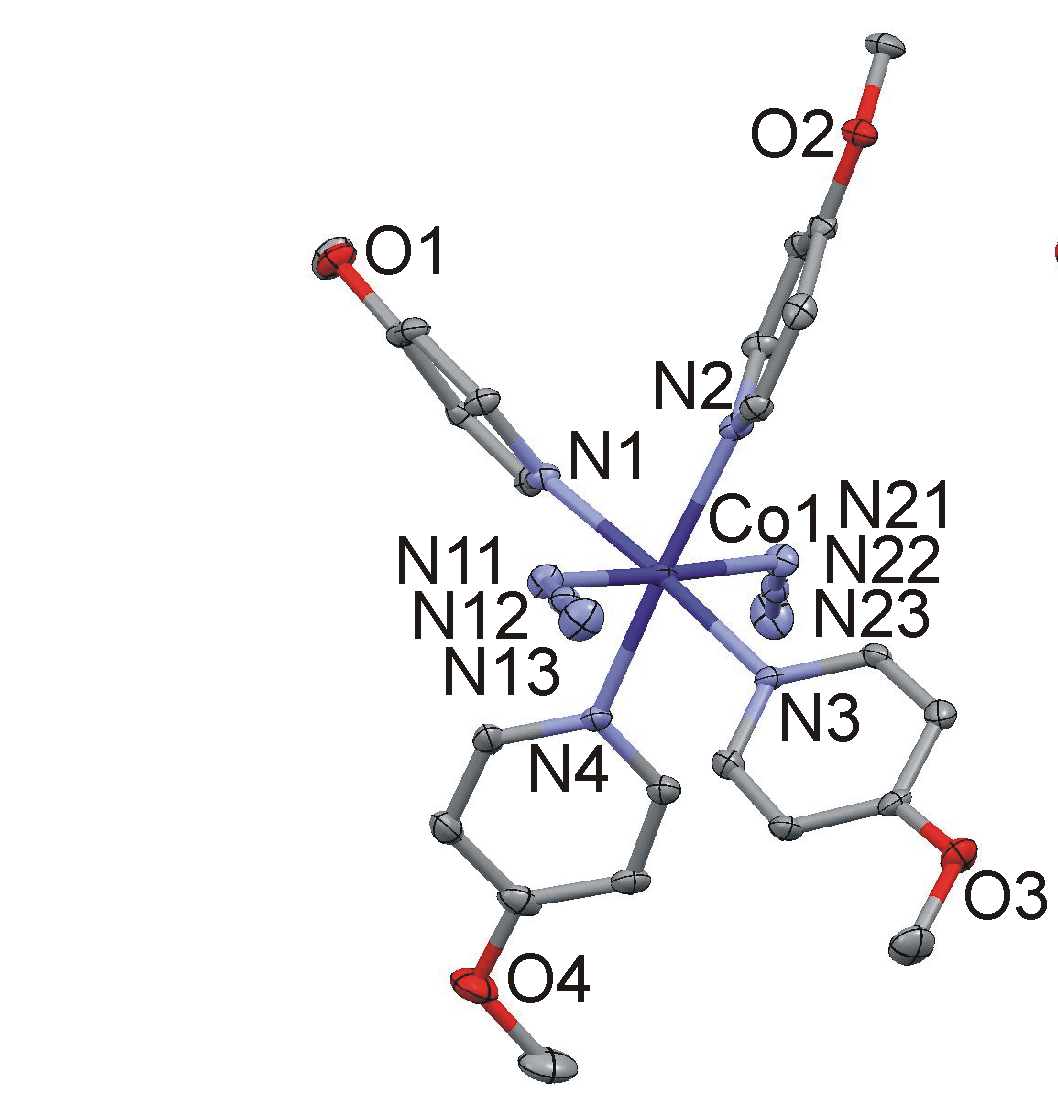
\includegraphics[width=1\textwidth]{figures/CO_4MOP_FIGm11.png}
\caption[Perspective view of \ce{[Co(N_3)_2(4-MeOpy)_4]}]{Perspective view of \ce{[Co(N_3)_2(4-MeOpy)_4]} with the atom numbering scheme.}
\label{fig:CoA4MOP_pv}
\vspace{\floatsep}
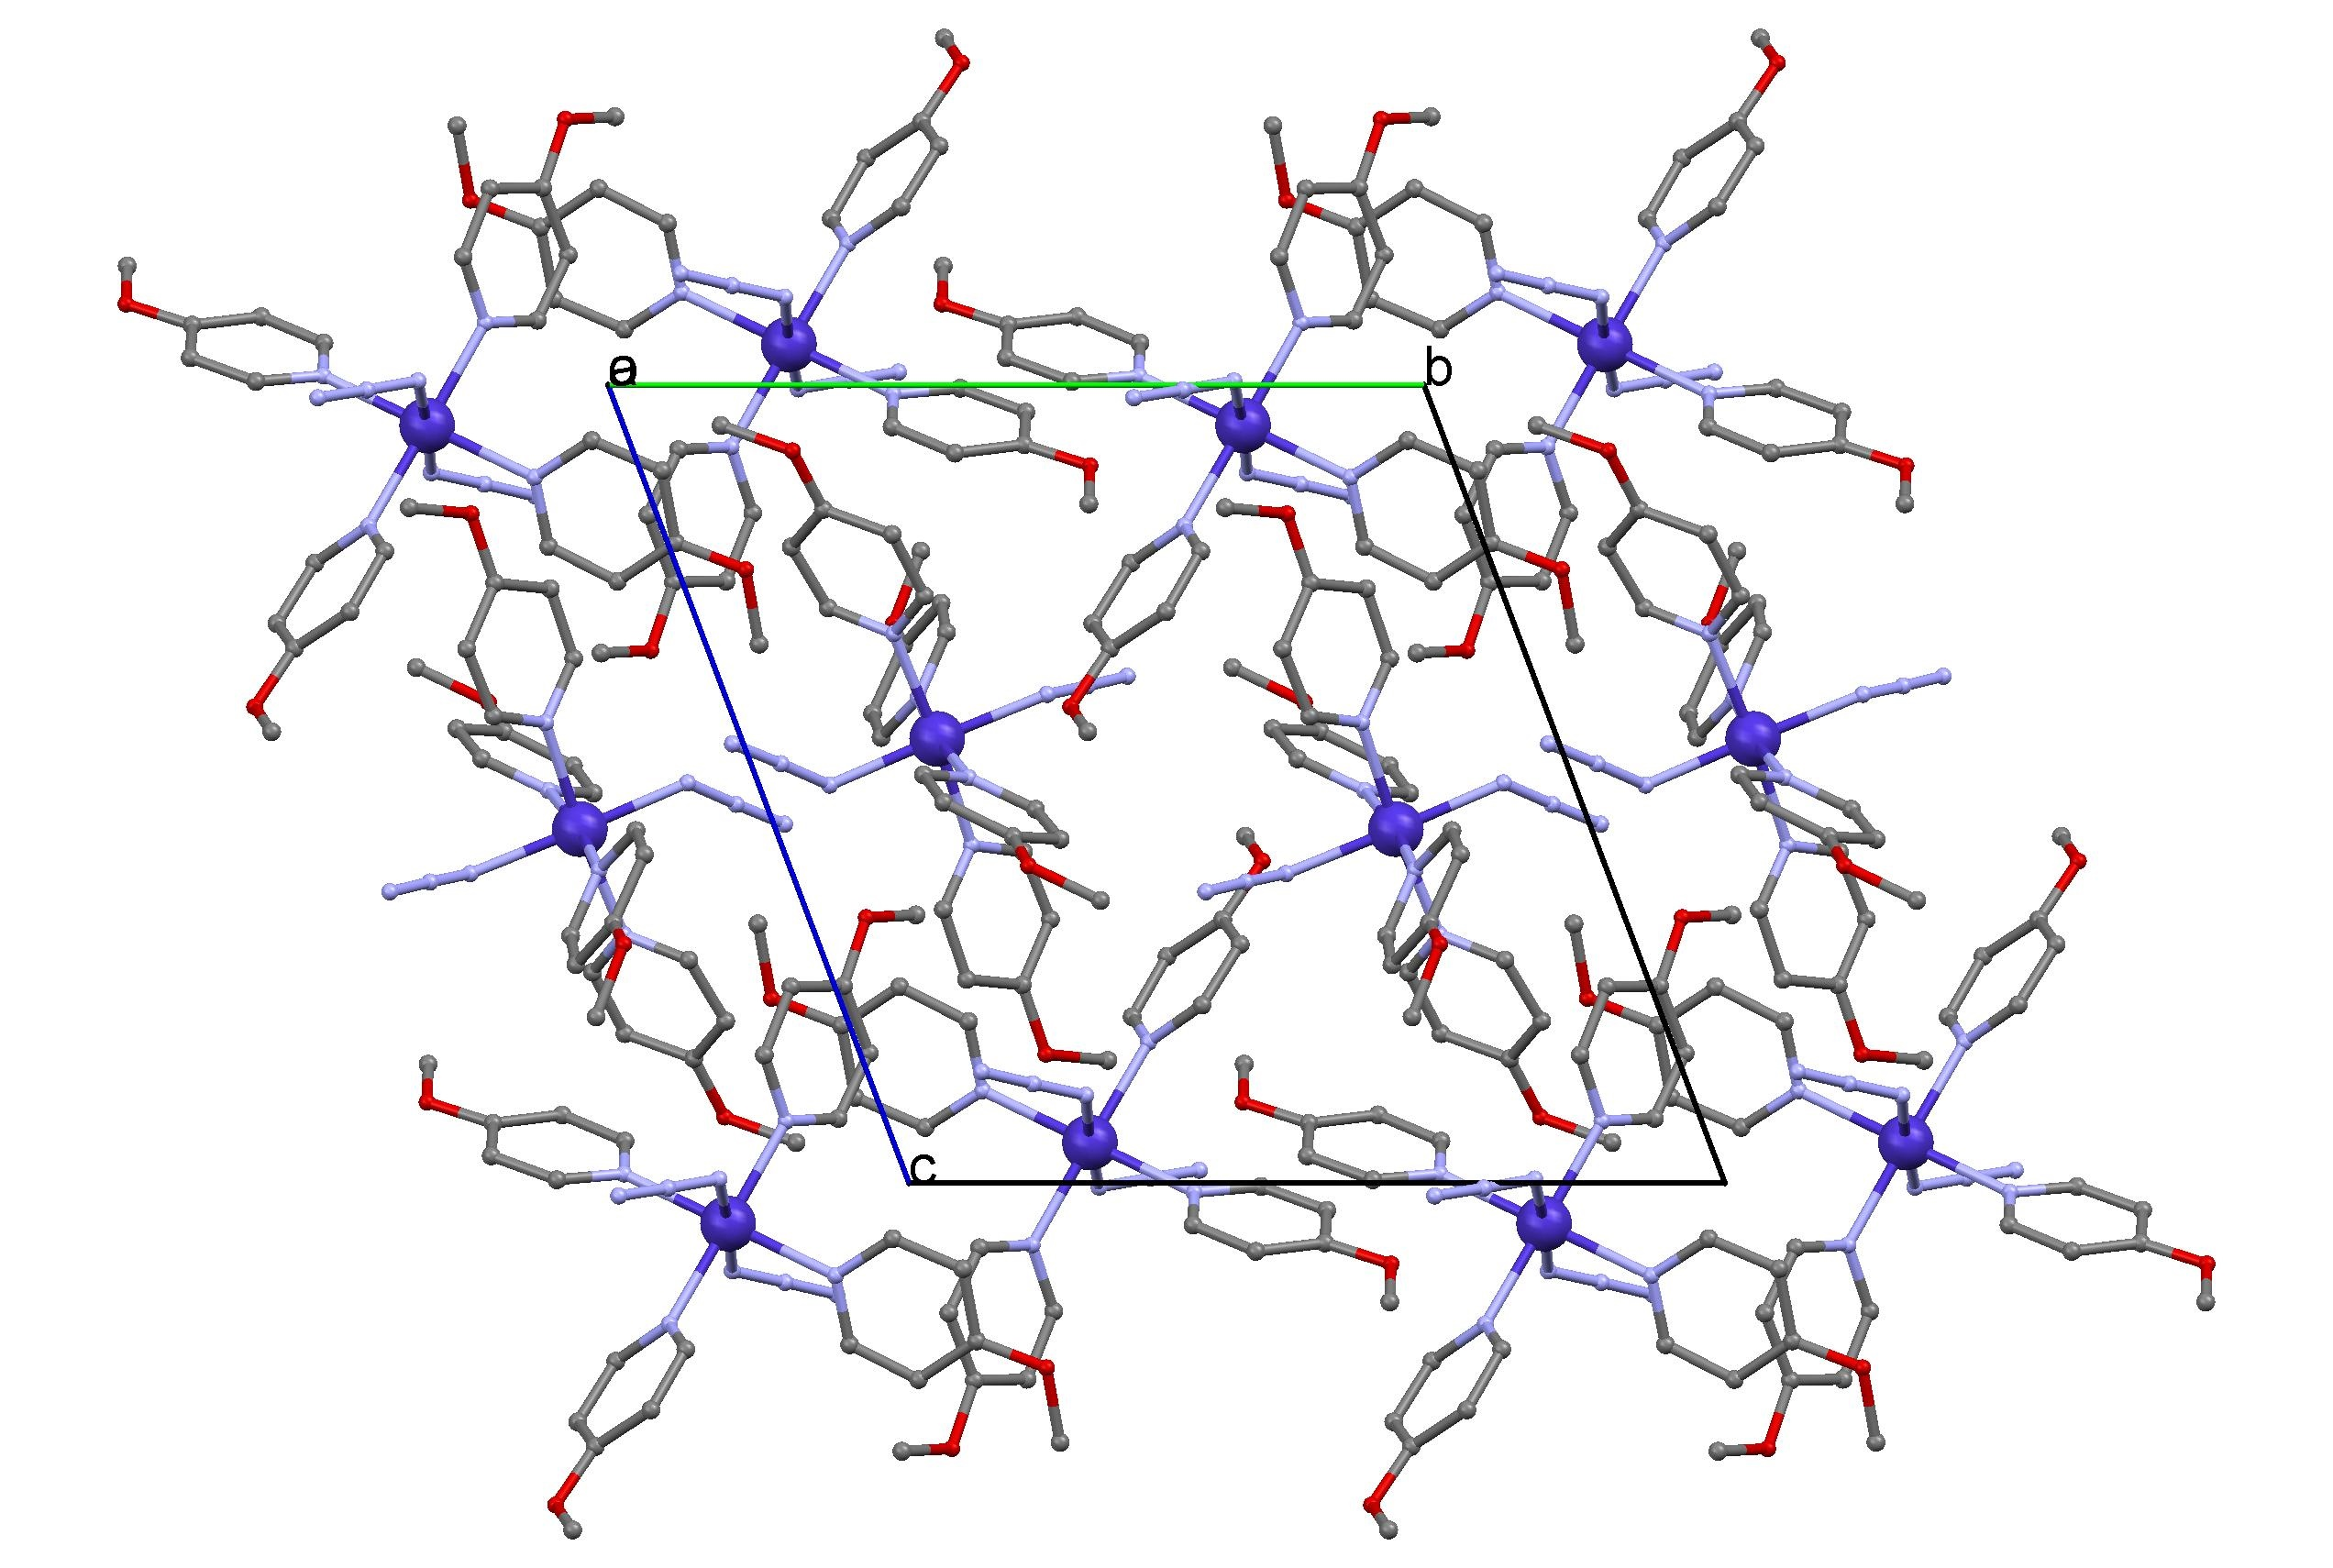
\includegraphics[width=1\textwidth]{figures/co_4mop_CA.jpg}
\caption{Packing view of \ce{[Co(N_3)_2(4-MeOpy)_4]}.}
\label{fig:CoA4MOP_packv}
\end{figure}




\begin{table}
\centering
\captionabove{Crystallographic data and processing parameter of \ce{[Co(N_3)_2(4-MeOpy)_4]}}
\begin{tabular}{ | l |  l | }
\hline
Empirical formula & \ce{C_{24}H_{28}CoN_{10}O_{4}}\\
\hline
Formula mass & 579.49\\
\hline
System & triclinic\\
\hline
Space group & P-1\\
\hline
a ({\AA}) & 12.7449(5)\\
\hline
b ({\AA}) & 14.6263(6)\\
\hline
c ({\AA}) & 16.4750(6)\\
\hline
$\alpha$ ($^\circ$) & 70.309(2)\\
\hline
$\beta$ ($^\circ$) & 68.118(2)\\
\hline
$\gamma$ ($^\circ$) & 88.507(2)\\
\hline
V (\AA$^{3}) $  & 2665.58(19)\\
\hline
Z & 4\\
\hline
T (K) & 100(2)\\
\hline
$\mu$ (mm$^{-1}$) & 0.695\\
\hline
 D$_{calc}$ (Mg/m$^{3}$) & 1.444\\
\hline
Crystal size (mm) & 0.23 x 0.17 x 0.10\\
\hline
$\theta$ max ($^\circ$) & 28.05\\
\hline
Data collected & 12857\\
\hline
Unique refl./ R$_{int}$ & 12857 / -----\\
\hline
Parameters & 712\\
\hline
Goodness-of-Fit on F$^{2}$ & 1.058\\
\hline
R1 / wR2 (all data) & 0.0608 /0.1495\\
\hline
Residual extrema (e/\AA$^{3}$) & 0.75 /-1.27\\
\hline
\end{tabular}
\label{ptbl:CoA4MOP}
\end{table}





\section{\ce{[Cu(N_3)_2(4-methoxypyridine)_2]_n}}
\subsection{Synthesis}
0.48 g \ce{Cu(NO_3)_2* 3 H_2O} (2 mmol), 0.26 g Na-azide (4 mmol) and 0.44 g 4-methoxy-pyridine (4 mmol) were dissolved in 50 mL distilled \ce{H_2O}. The solution was stirred for 2 hours  at 50$^\circ$C followed by a filtration of the resulting green solution. The mixture was stirred again for 55 minutes at the same temperature and then cooled down to room temperature. After 24 hours green needle-shaped crystals were obtained. Anal. Calculated for \ce{C_{12}H_{14}CuN_{8}O_{2}} (365.86 g/mol) : 39.40\% C; 3.86\% H; 30.63\% N; Found: 39.13 \% C; 3.87\% H; 30.52 \% N; IR (ATR, cm$^{-1}$): 2093 (s), 1616 (s), 1569 (m), 1512 (s), 1434 (m), 1301 (s), 1210 (s), 1062 (m), 1033 (s), 1009 (s), 822 (s), 660 (w), 602 (w), 576 (w), 533 (vs), 469 (m)


\begin{figure}[h!]
\centering
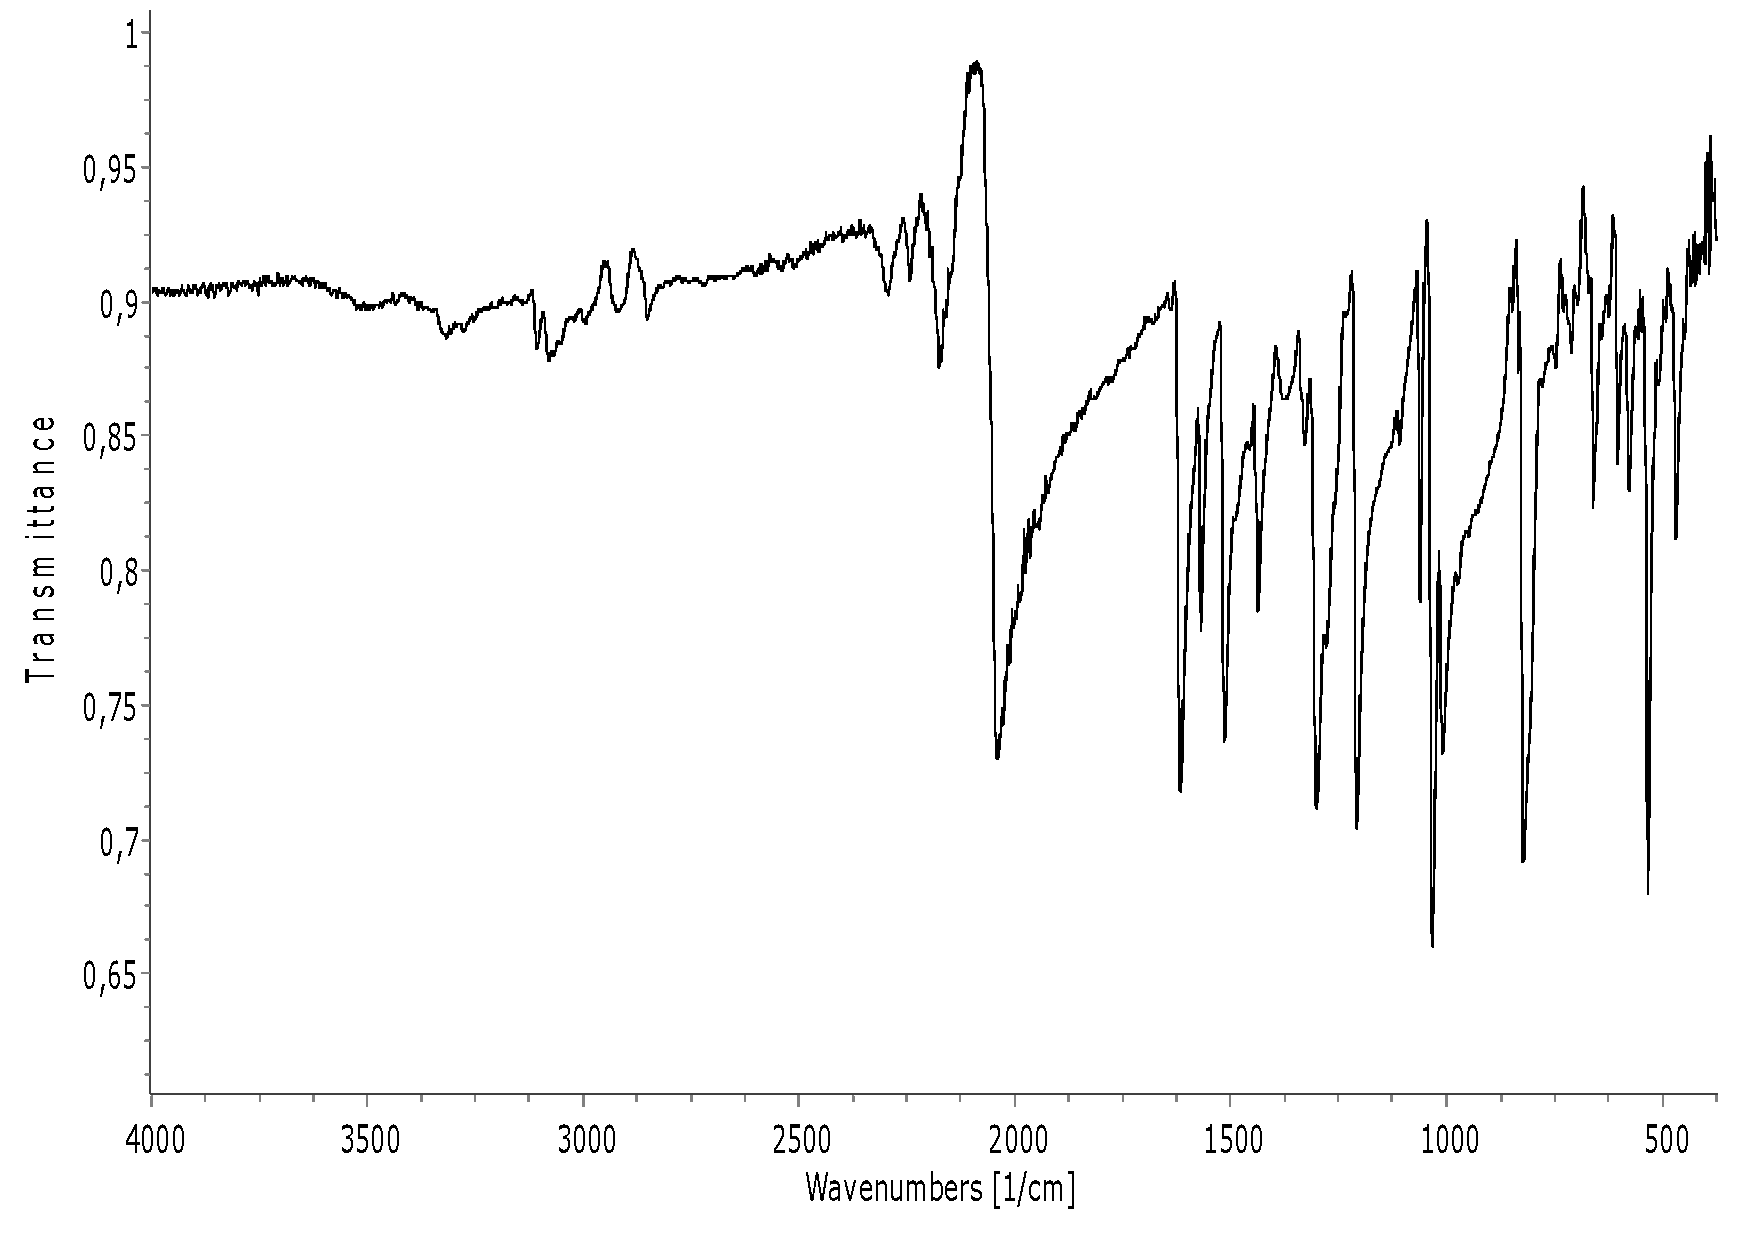
\includegraphics[width=1\textwidth]{figures/CuA4MOP-IR.pdf}
\caption{IR spectrum of \ce{[Cu(N_3)_2(4-MeOpy)_2]_n}}
\end{figure}

\subsection{Structural characterization}

A perspective view of \ce{[Cu(N_3)_2(4-MeOpy)_2]_n} is given in fig. \ref{fig:CuA4MOP_pv}, a packing view in fig. \ref{fig:CuA4MOP_packv} and selected bond parameters are summarized in table \ref{batab:CuA4MOP}. The Cu(1) metal center is located on an inversion center. It is coordinated via the pyridine N donor atom of two 4-MOP molecules in trans configuration and four N(11) atoms of azide groups. The latter act as bis-EO bridging ligands to generate polymeric chains of polyhedra along the a-axis of the triclinic unit cell. The \ce{CuN_6} chromophore may be described as axially elongated square bipyramid with longer Cu(1)-N(11b) bond distance of 2.736(4) \AA, and shorter bond distances of 2.022(4) and 2.009(3) \AA, for Cu(1)-N(11) and Cu(1)-N(1), respectively. The following bond angles are observed for the bis-EO azide bridging system: N(11)-Cu(1)-N(11c ) = 79.56(14), Cu(1)-N(11)-Cu(1c) = 100.4(2), Cu(1)-N(11)-N(12) = 121.3(3) and N(11)-N(12)-N(13) = 178.0(4)$^\circ$. The intra-chain Cu-Cu distance is 3.6846(14) and the shortest inter-chain metal-metal separation is 7.369(3) \AA.
\renewcommand{\arraystretch}{1.3}

\begin{table}[ htpb!]
\centering
\captionabove{Selected bond lengths (\AA) and angles ($^\circ$) for \ce{[Cu(N_3)_2(4-MeOpy)_2]_n}}
\begin{tabular}{|l|l|l|l|}
\hline
Cu(1)-N(1a) & 2.009(3) & Cu(1)-N(11b) & 2.736(4)\\
\hline
Cu(1)-N(11a) & 2.022(4) & N(11)-N(12) & 1.197(5)\\
\hline
N(12)-N(13) & 1.162(5) &  & \\
\hline
\hline
N(1a)-Cu(1)-N(11a) & 91.46(14) & N(11)-Cu(1)-N(11c) & 79.56(4)\\
\hline
N(1)-Cu(1)-N(1a) & 180.0 & N(11)-Cu(1)-N(11a) & 180.0\\
\hline
N(11b)-Cu(1)-N(11c) & 180.0 & N(11)-Cu(1)-N(11b) & 100.44(14)\\
\hline
Cu(1)-N(11)-N(12) & 121.3(3) & N(11)-N(12)-N(13) & 178.0(4)\\
\hline
\end{tabular}
\label{batab:CuA4MOP}
\end{table}



\begin{figure}[!htpb]
\centering
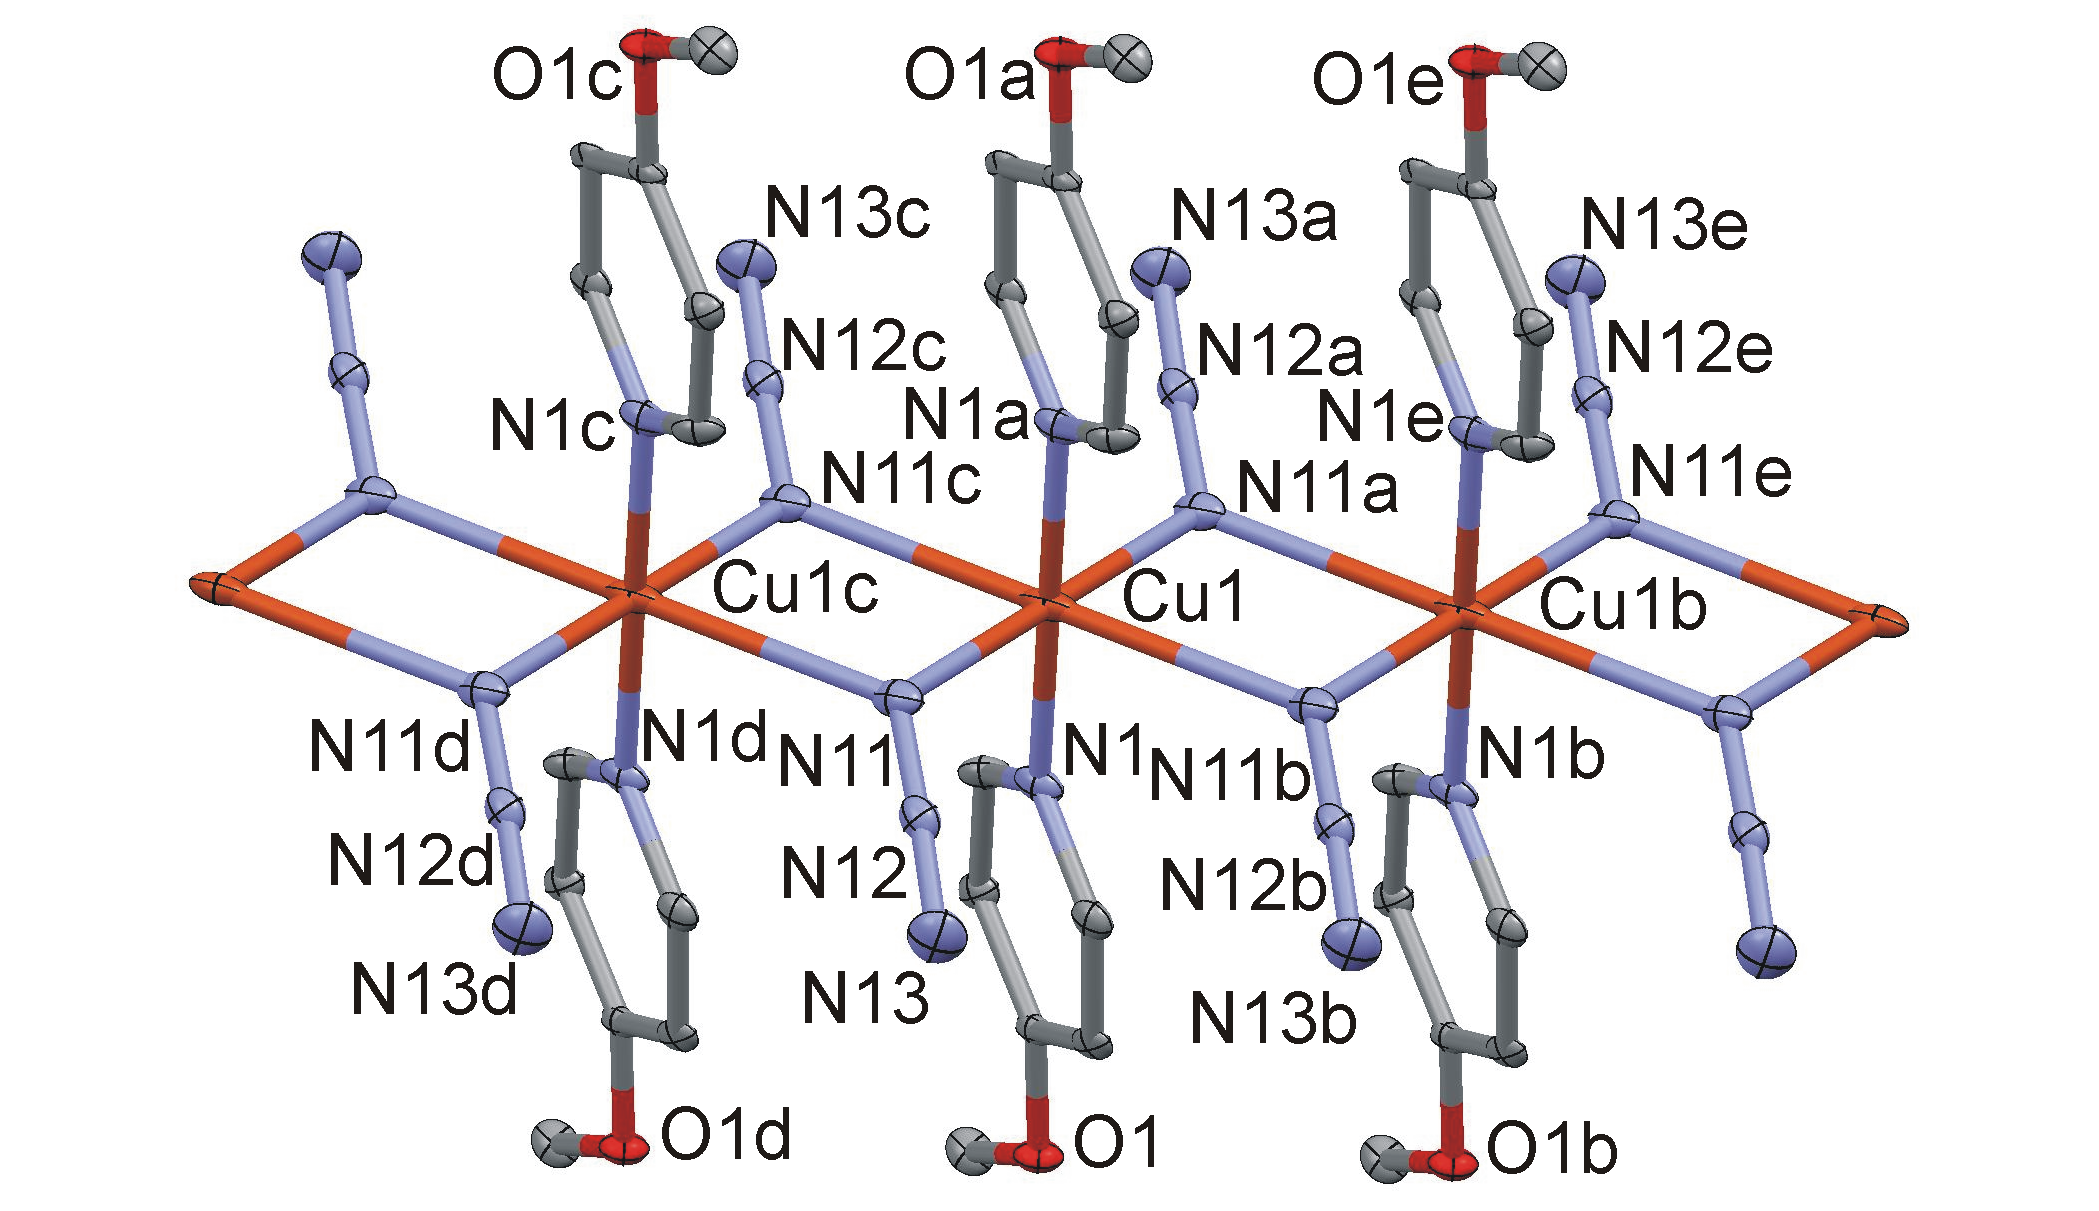
\includegraphics[width=0.95\textwidth]{figures/CuA4MOP_FIGm12.png}
\caption[Perspective view of \ce{[Cu(N_3)_2(4-MeOpy)_2]_n}]{Perspective view of a section of the polymeric chain of \ce{[Cu(N_3)_2(4-MeOpy)_2]_n} with the atom numbering scheme. Symmetry code:(a) 1-x,1-y,1-z; (b) -1+x,y,z; (c) 2-x,1-y,1-z; (d) 1+x,y,z; 
(e) –x,1-y,1-z.}
\label{fig:CuA4MOP_pv}
\vspace{\floatsep}
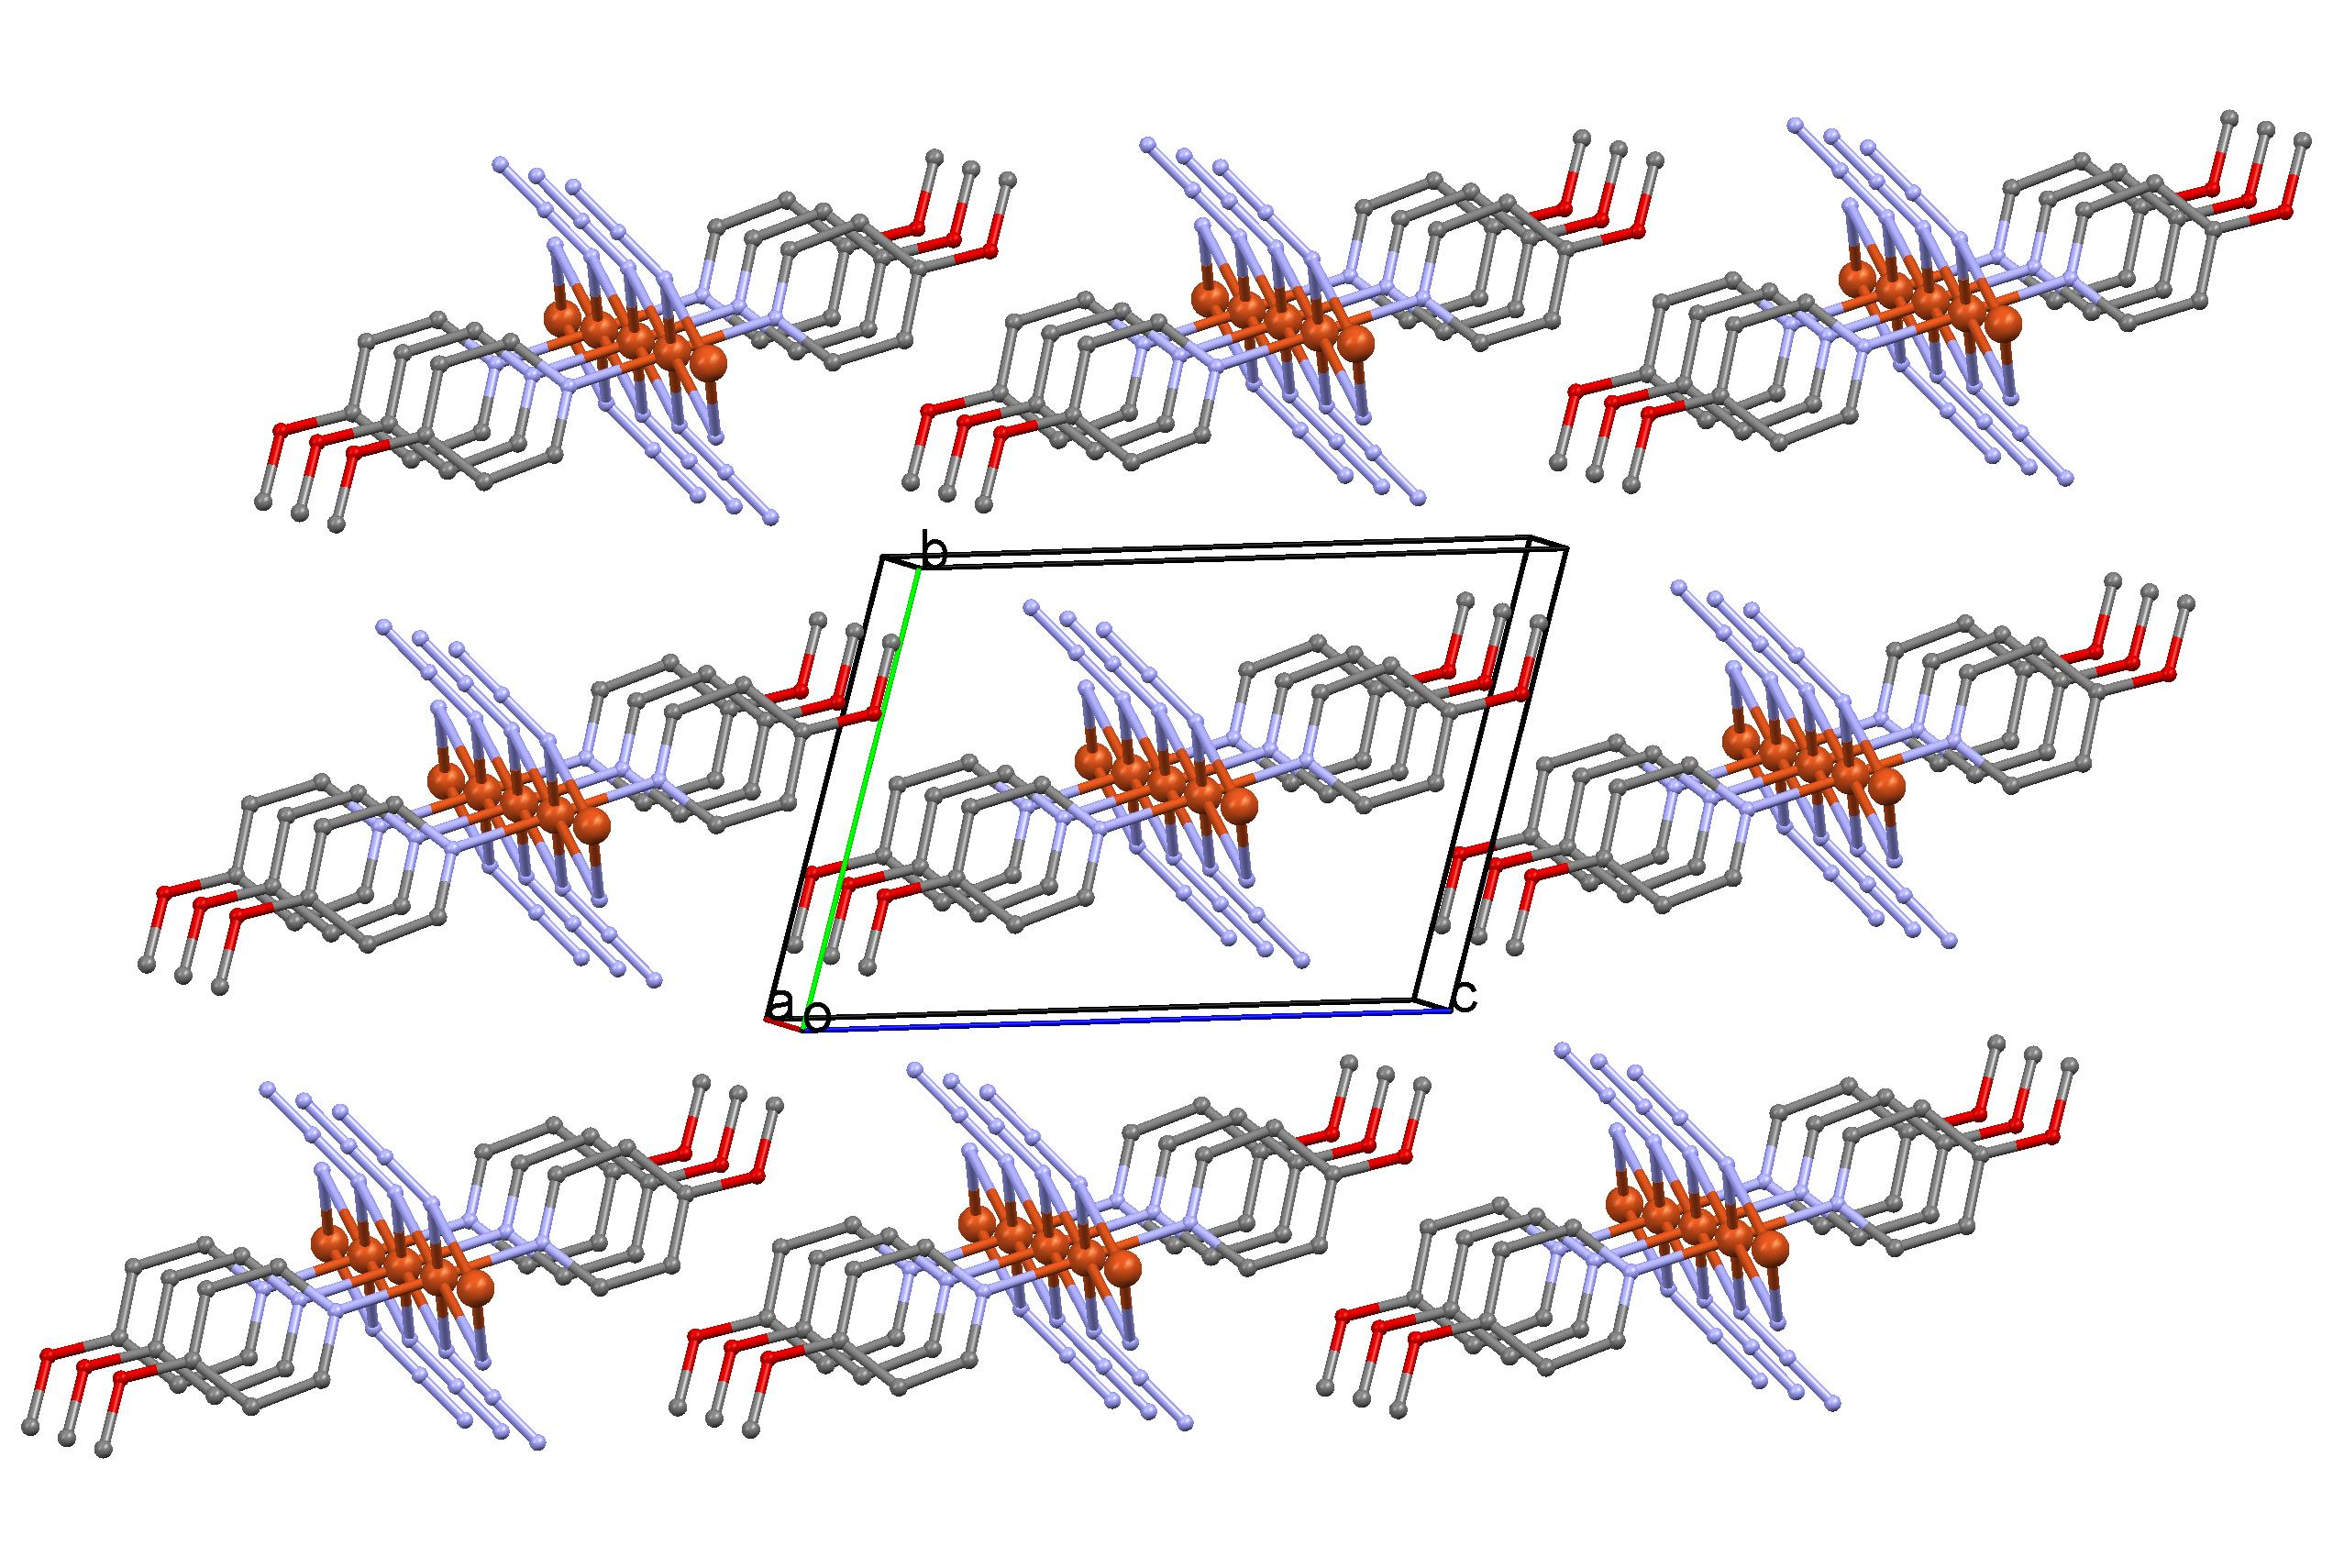
\includegraphics[width=0.95\textwidth]{figures/CuA4MOP_CA.png}
\caption{Packing plot  of \ce{[Cu(N_3)_2(4-MeOpy)_2]_n}.}
\label{fig:CuA4MOP_packv}
\end{figure}


\begin{table}
\centering
\captionabove{Crystallographic data and processing parameter of \ce{[Cu(N_3)_2(4-MeOpy)_2]_n}}
\begin{tabular}{ | l |  l | }
\hline
Empirical formula & \ce{C_{12}H_{14}CuN_{8}O_{2}}\\
\hline
Formula mass & 365.86\\
\hline
System & triclinic\\
\hline
Space group & P-1\\
\hline
a ({\AA}) & 3.6846(11)\\
\hline
b ({\AA}) & 8.755(3)\\
\hline
c ({\AA}) & 12.244(4)\\
\hline
$\alpha$ ($^\circ$) & 73.020(14)\\
\hline
$\beta$ ($^\circ$) & 85.062(16)\\
\hline
$\gamma$ ($^\circ$) & 83.034(16)\\
\hline
V (\AA$^{3}) $  & 374.4(2)\\
\hline
Z & 1\\
\hline
T (K) & 100(2)\\
\hline
$\mu$ (mm$^{-1}$) & 1.482\\
\hline
 D$_{calc}$ (Mg/m$^{3}$) & 1.623\\
\hline
Crystal size (mm) & 0.32 x 0.15 x 0.09\\
\hline
$\theta$ max ($^\circ$) & 26.98\\
\hline
Data collected & 10906\\
\hline
Unique refl./ R$_{int}$ & 1602 / 0.1163\\
\hline
Parameters & 107\\
\hline
Goodness-of-Fit on F$^{2}$ & 1.149\\
\hline
R1 / wR2 (all data) & 0.0668 /0.1567\\
\hline
Residual extrema (e/\AA$^{3}$) & 1.39 /-1.74\\
\hline
\end{tabular}

\label{ptab:CuA4MOP}

\end{table}



\section{\ce{[Zn(N_3)_2(4-methoxypyridine)_2]}}
\subsection{Synthesis}
\ce{Zn(NO_3)_2*6 H_2O} (0.59 g, 2 mmol), \ce{NaN_3} (0.13 g, 2 mmol) and  4-methoxy-pyridine (0.22 g, 2 mmol) were added in 40 mL distilled \ce{H_2O}. The solution was heated up to 80$^\circ$C  and stirred for 2 hours. After filtration the clear solution was stirred again for 30 minutes at the same temperature and then cooled down to RT. After 3 days needle-shaped white crystals were obtained. Anal. Calculated for \ce{C_{12}H_{14}N_8O_2Zn} (367.70 g/mol) : 39.20\% C; 3.84\% H; 30.48\% N; Found: 38.96\% C; 3.87\% H; 30.33 \% N; IR (ATR, cm$^{-1}$): 2094 (s), 2058 (s), 1615 (s), 1568 (s), 1513 (s), 1439 (s), 1355 (m), 1298 (s), 1210 (s), 1061 (m), 1031 (s), 819 (s), 731 (w), 659 (w), 580 (w), 535 (s), 465 (m)

\begin{figure}[h!]
\centering
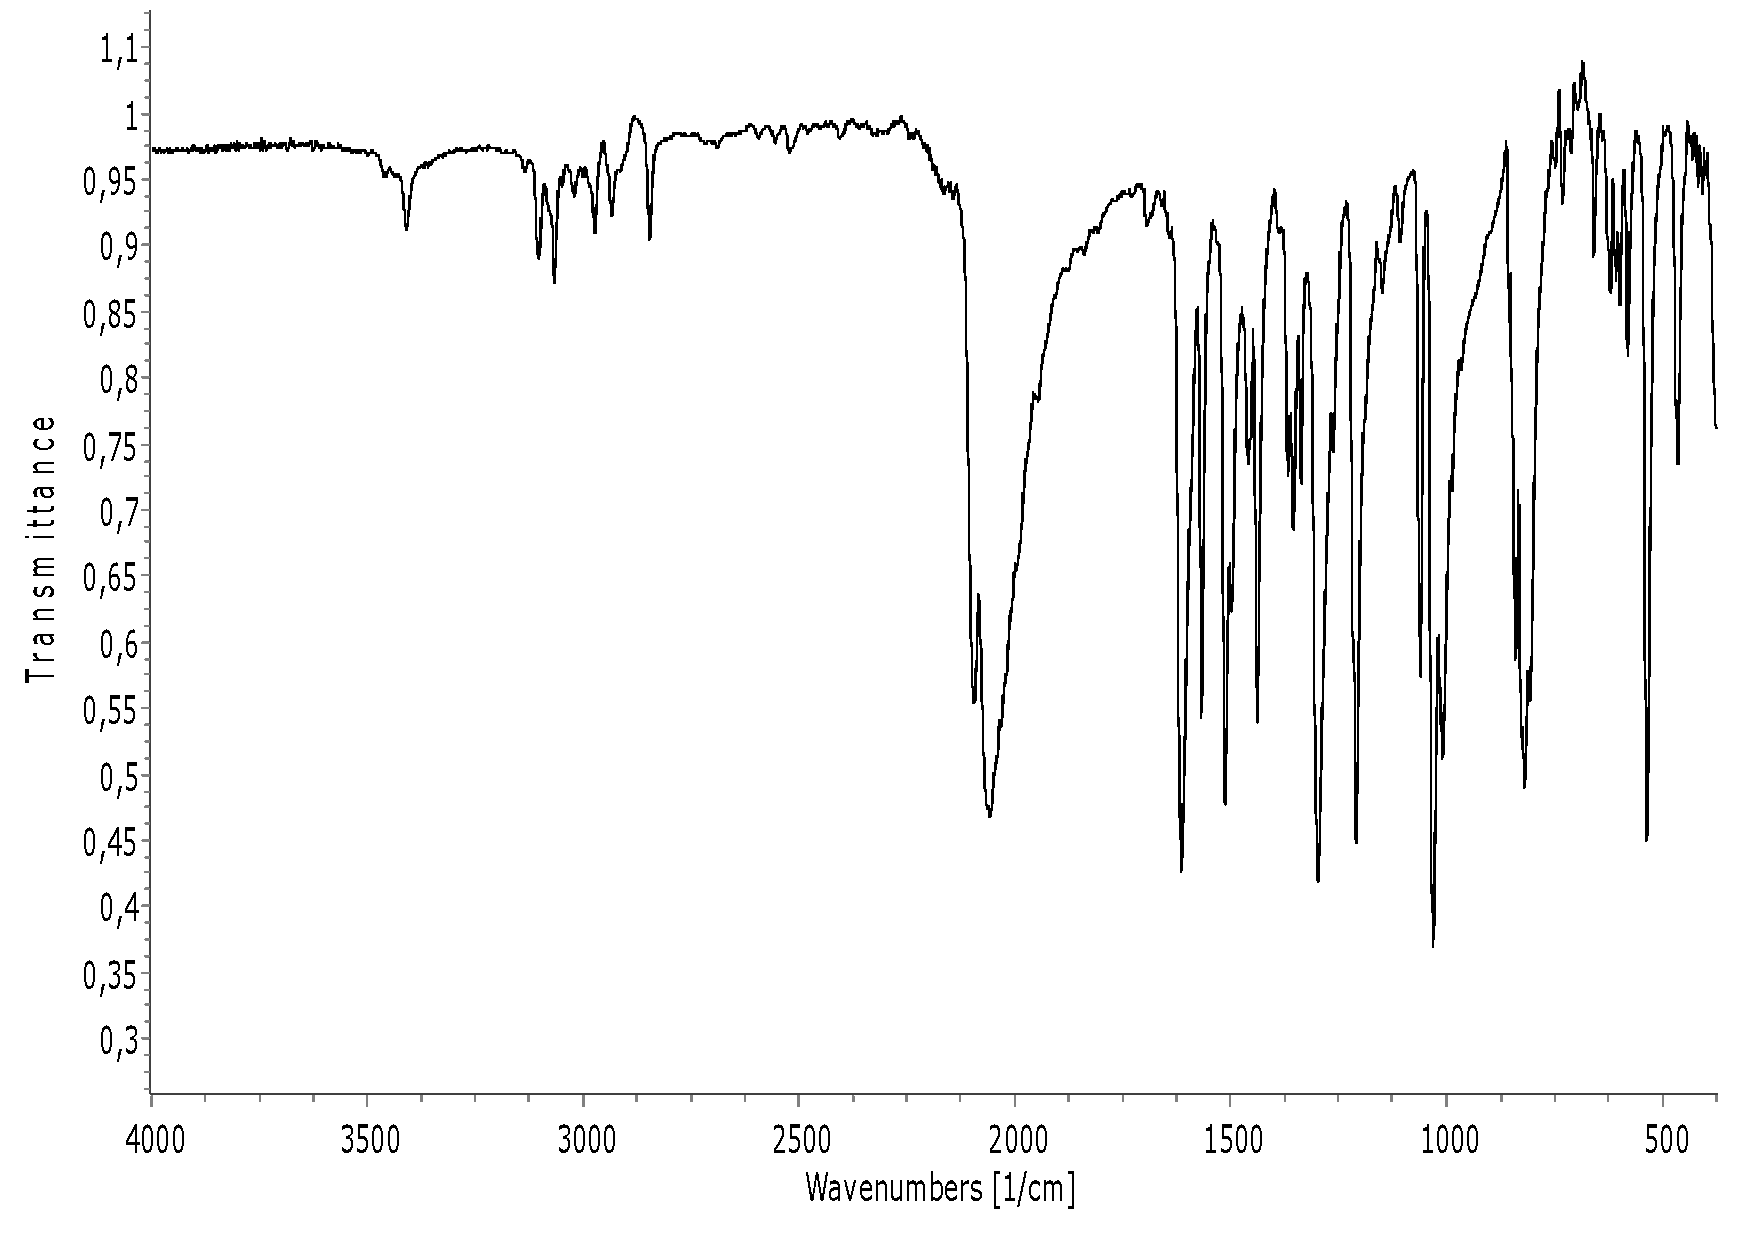
\includegraphics[width=1\textwidth]{figures/ZnA4MOP-IR.pdf}
\caption{IR spectrum of \ce{[Zn(N_3)_2(4-MeOpy)_2]}}
\end{figure}

\subsection{Structural characterization}

The crystal structure of \ce{[Zn(N_3)_2(4-MeOpy)_2]} consists of mononuclear and neutral Zn(II) complexes, as depicted in figure \ref{fig:ZnA4MOP_pv} (perspective view) and figure \ref{fig:ZnA4MOP_packv} (packing view). Selected bond parameters are listed in table \ref{batab:ZnA4MOP}.  Zn(1) is tetrahedrally coordinated by N(11) and N(21) of two terminal azido groups, further by N(1) and N(2) atoms of two neutral \ce{4-methoxypyridine} molecules. The Zn-N bond lengths range from 1.9330(14) to 2.0311(13) \AA, and the bond angles within the \ce{ZnN_4} tetrahedron vary from 100.25(6) to 128.66(6)$^\circ$. The bond parameters of the terminal azido groups are: Zn-N-N = 138.48(12) and 142.44(12)$^\circ$, N-N-N = 177.17(17) and 174.52(17)$^\circ$, N(x1)-N(x2) = 1.182(2) and 1.1918(19) \AA, N(x2)-N(x3) = 1.156(2) and 1.148(2) \AA.The shortest metal-metal separation is 5.3288(7) \AA. 

\begin{table}[htpb!]
\centering
\captionabove{Selected bond lengths (\AA) and angles ($^\circ$) for \ce{[Zn(N_3)_2(4-MeOpy)_2]}}
\begin{tabular}{|l|l|l|l|}
\hline
Zn(1)-N(11) & 1.9714(14) & Zn(1)-N(1) & 2.0311(13)\\
\hline
Zn(1)-N(21) & 1.9330(14) & Zn(1)-N(2) & 2.0192(13)\\
\hline
N(11)-N(12) & 1.182(2) & N(12)-N(13) & 1.156(2)\\
\hline
N(21)-N(22) & 1.1918(19) & N(22)-N(23) & 1.148(2)\\
\hline
\hline
N(11)-Zn(1)-N(21) & 128.66(6) & N(1)-Zn(1)-N(21) & 101.00(5)\\
\hline
N(2)-Zn(1)-N(21) & 110.32(6) & N(1)-Zn(1)-N(11) & 100.25(6)\\
\hline
N(2)-Zn(1)-N(11) & 104.01(6) & N(1)-Zn(1)-N(2) & 111.79(5)\\
\hline
Zn(1)-N(11)-N(12) & 138.48(12) & N(11)-N(12)-N(13) & 177.17(17)\\
\hline
Zn(1)-N(21)-N(22) & 142.44(12) & N(21)-N(22)-N(23) & 174.52(17)\\
\hline
\end{tabular}

\label{batab:ZnA4MOP}
\end{table}



\begin{figure}[!htpb]
\centering
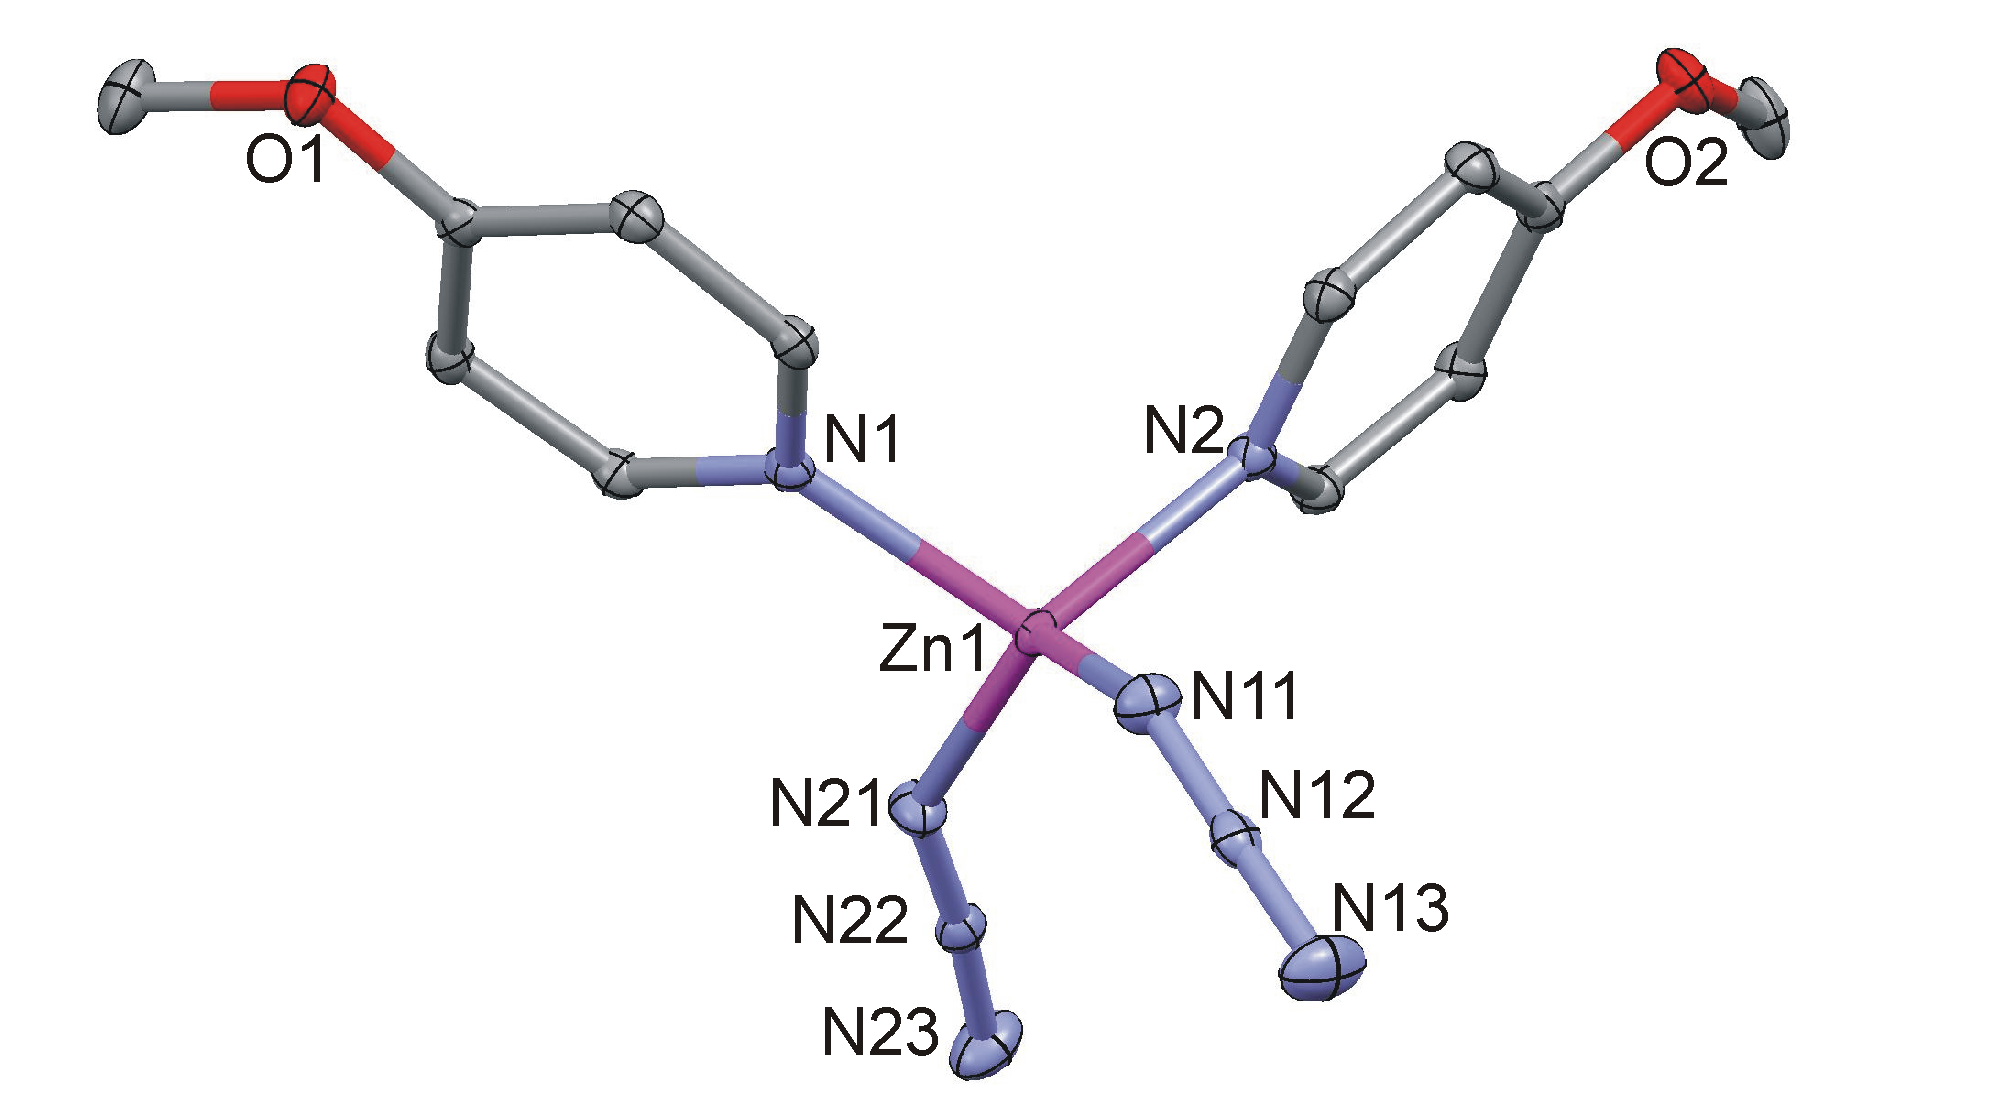
\includegraphics[width=1\textwidth]{figures/Zn_4OMP_FIGm11.png}
\caption[Perspective view of \ce{[Zn(N_3)_2(4-MeOpy)_2]}]{Perspective view of \ce{[Zn(N_3)_2(4-MeOpy)_2]} with the atom numbering scheme. Symmetry codes: (‘): -x,y,-z+1/2; (“): 1-x,y,-z+1/2.}
\label{fig:ZnA4MOP_pv}
\vspace{\floatsep}
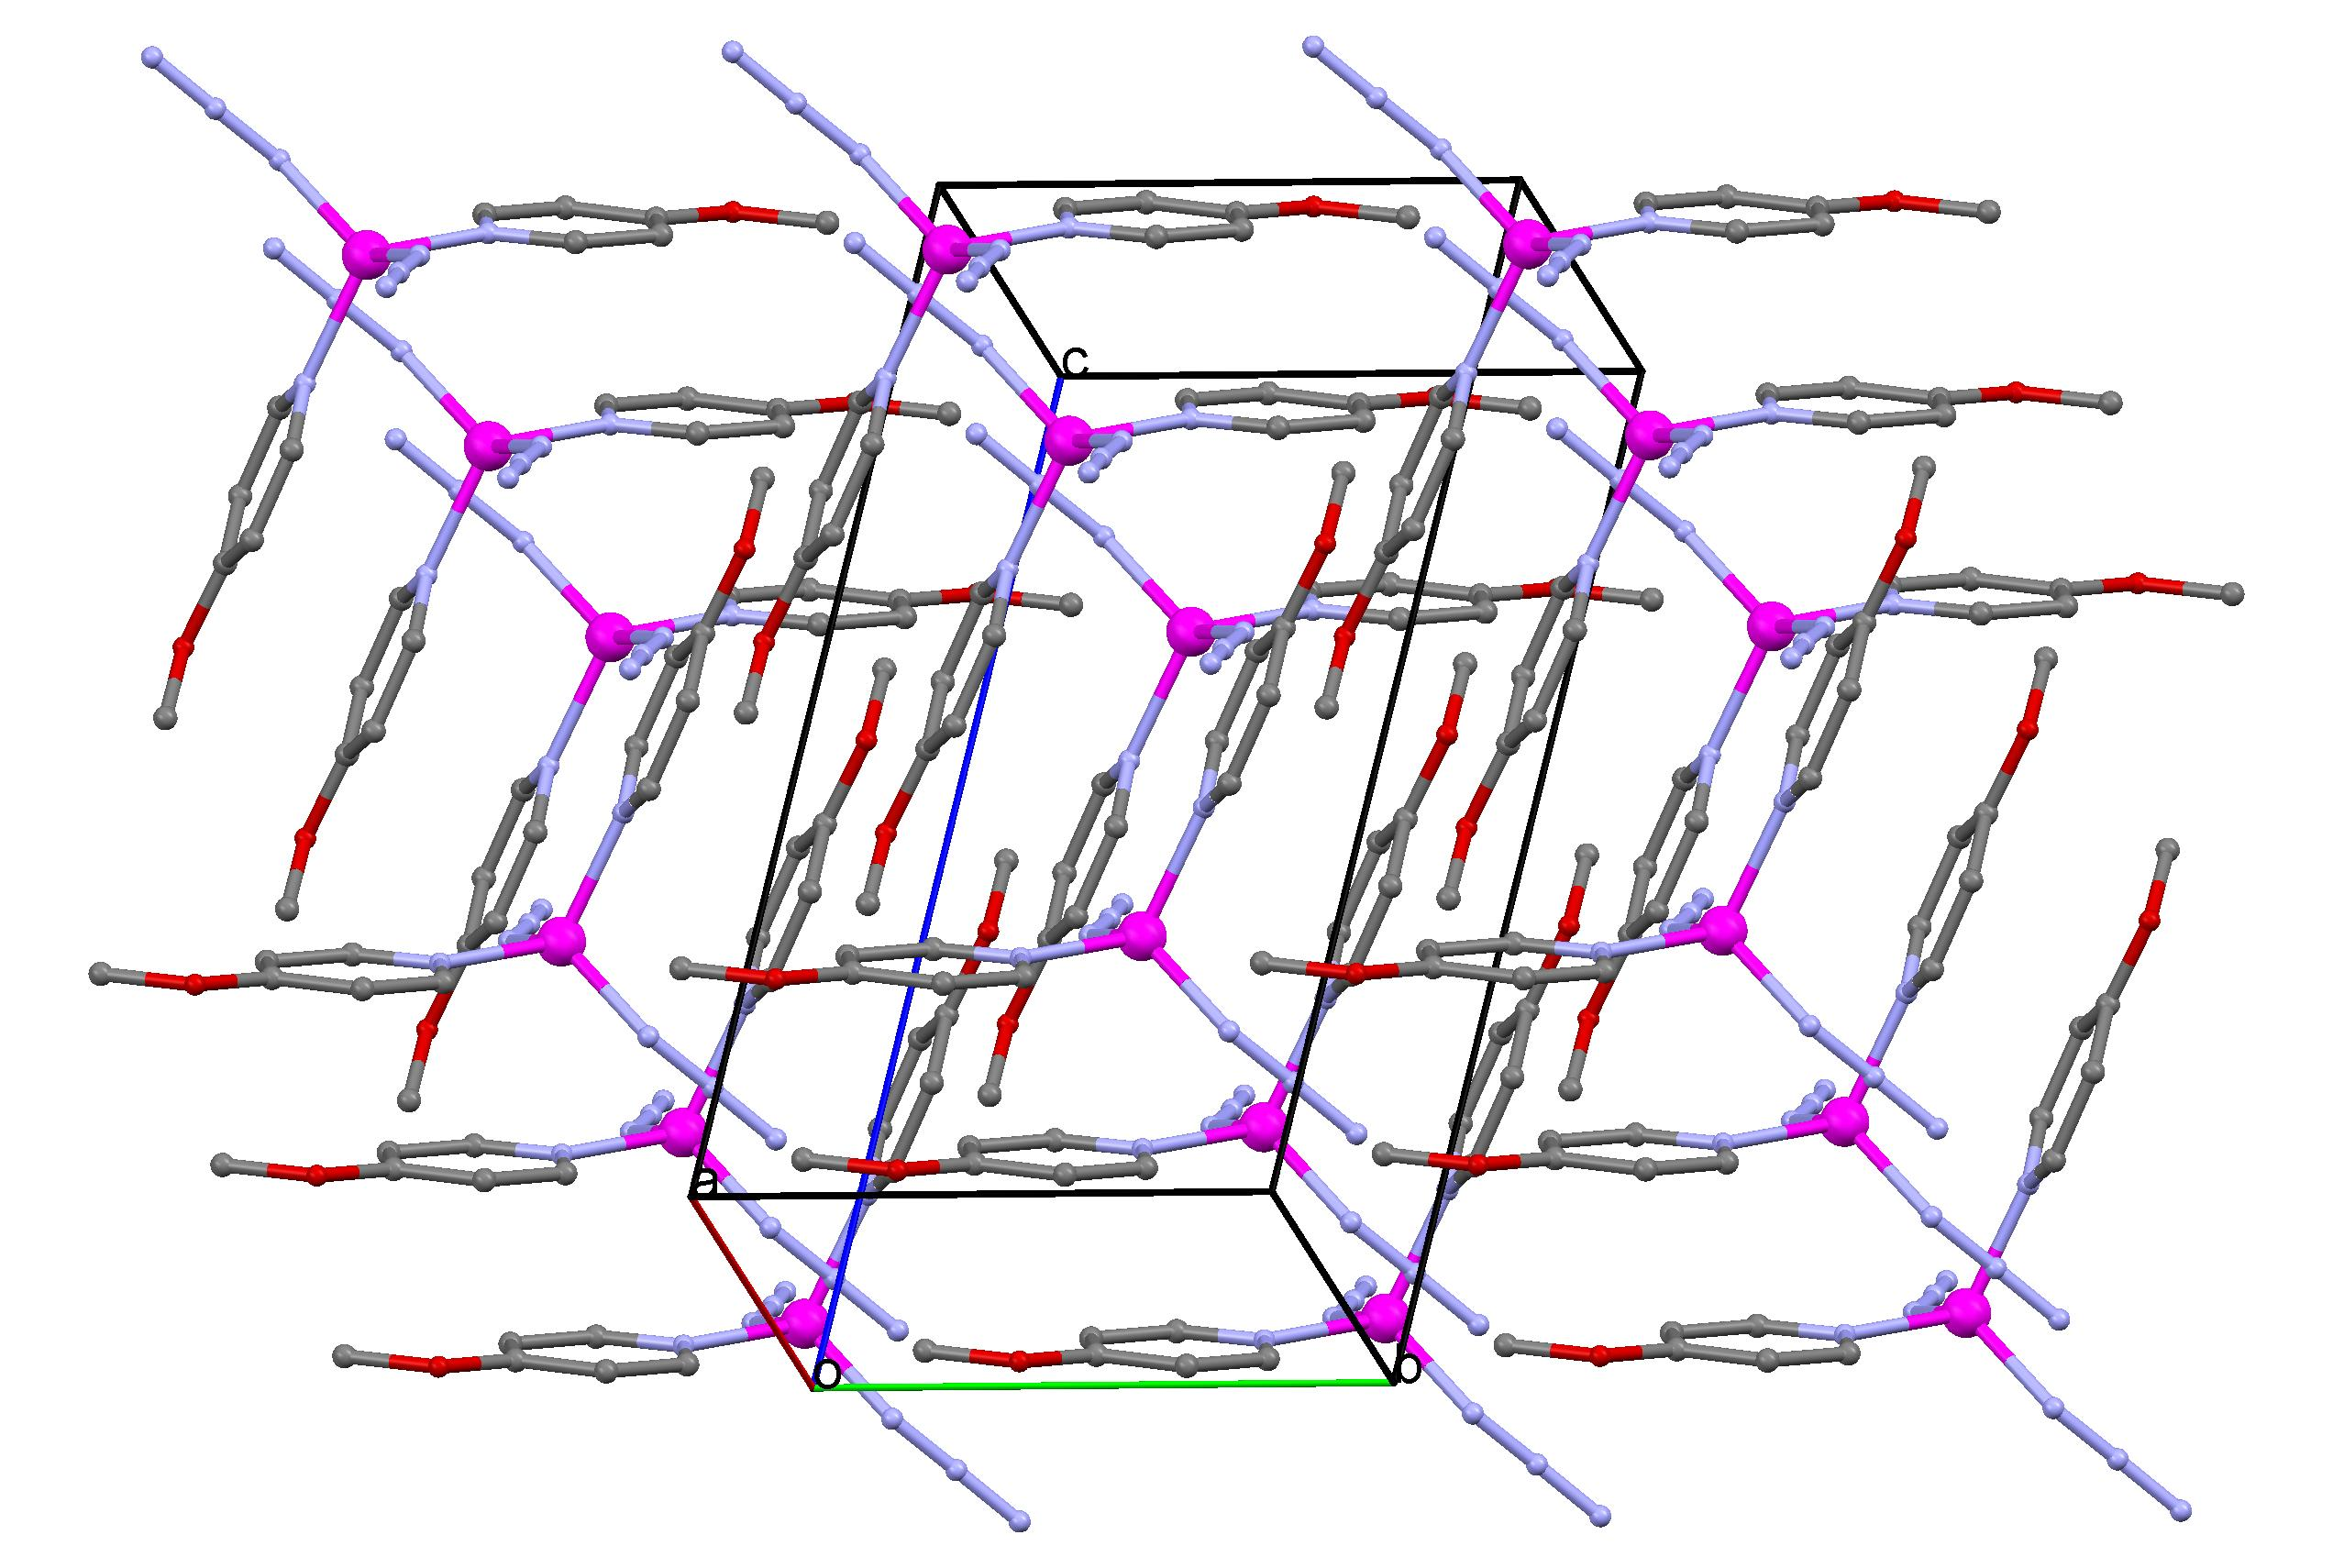
\includegraphics[width=1\textwidth]{figures/zn_A4meop_CA.png}
\caption{Packing view of \ce{[Zn(N_3)_2(4-MeOpy)_2]}.}
\label{fig:ZnA4MOP_packv}
\end{figure}

\renewcommand{\arraystretch}{1.5}
\begin{table}
\centering
\captionabove{Crystallographic data and processing parameter of \ce{[Zn(N_3)_2(4-MeOpy)_2]}}
\begin{tabular}{ | l |  l | }
\hline
Empirical formula & \ce{C_{12}H_{14}N_{8}O_{2}Zn}\\
\hline
Formula mass & 367.70\\
\hline
System & triclinic\\
\hline
Space group & P-1\\
\hline
a ({\AA}) & 5.3288(7)\\
\hline
b ({\AA}) & 9.751(1)\\
\hline
c ({\AA}) & 15.1580(14)\\
\hline
$\alpha$ ($^\circ$) & 88.877(3)\\
\hline
$\beta$ ($^\circ$) & 82.068(3)\\
\hline
$\gamma$ ($^\circ$) & 78.448(3)\\
\hline
V (\AA$^{3}) $  & 764.26(15)\\
\hline
Z & 2\\
\hline
T (K) & 100(2)\\
\hline
$\mu$ (mm$^{-1}$) & 1.630\\
\hline
 D$_{calc}$ (Mg/m$^{3}$) & 1.598\\
\hline
Crystal size (mm) & 0.32 x 0.22 x 0.18\\
\hline
$\theta$ max ($^\circ$) & 26.35\\
\hline
Data collected & 6131\\
\hline
Unique refl./ R$_{int}$ & 3069 / 0.0172\\
\hline
Parameters & 210\\
\hline
Goodness-of-Fit on F$^{2}$ & 1.063\\
\hline
R1 / wR2 (all data) & 0.0220 /0.0542\\
\hline
Residual extrema (e/\AA$^{3}$) & 0.27 /-0.40\\
\hline
\end{tabular}

\label{ptab:ZnA4MOP}


\end{table}



\section{\ce{[Co(OCN)_2(4-methoxypyridine)_4]}}
\subsection{Synthesis}
0.58 g \ce{Co(NO_3)_2 * 6 H_2O} (2 mmol), 0.32 g KOCN (4 mmol) and 0.87 g 4-methoxy-pyridine (8 mmol) were dissolved in 35 mL distilled \ce{H_2O}. The solution was heated up to $70^\circ$C  and stirred for 1 hour and 30 minutes. After filtration the pink solution was stirred again for 45 minutes at the same temperature and then cooled to RT. After 24 hours pink needle-shaped crystals were obtained. Anal. Calculated for \ce{C_{26}H_{28}CoN_{6}O_{6}} (579.47 g/mol) : 53.89\% C; 4.87\% H; 14.50\% N;
Found: 53.66 \% C; 4.84\% H; 14.52 \% N;
IR (ATR, cm$^{-1}$): 2190 (s), 1604 (s), 1565 (m), 1497 (m), 1441 (m), 1426 (m), 1318 (w), 1288 (s), 1205 (s), 1023 (s), 1001 (m), 817 (m), 617 (s), 567 (w), 536 (s), 457 (m)

\begin{figure}[h!]
\centering
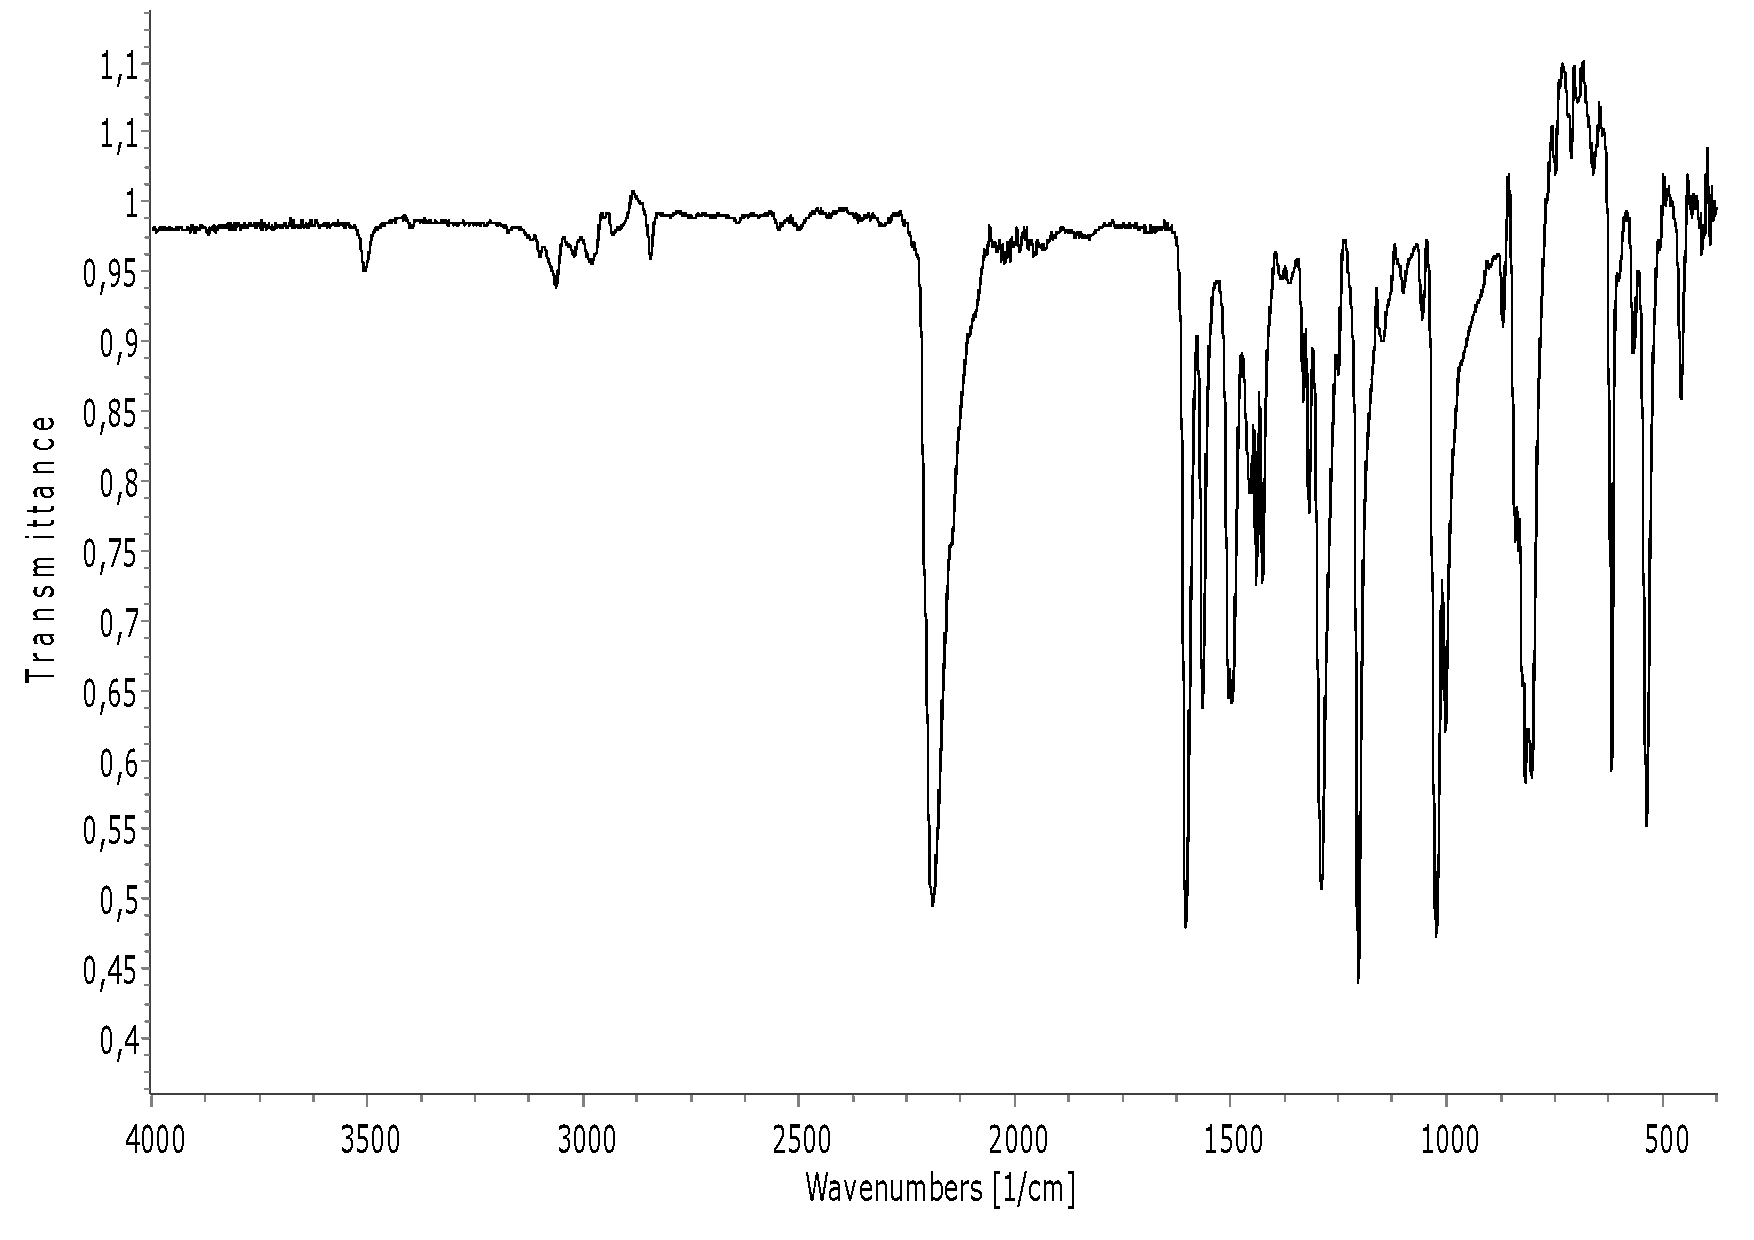
\includegraphics[width=1\textwidth]{figures/CoO4MOP-IR.pdf}
\caption{IR spectrum of \ce{[Co(OCN)_2(4-MeOpy)_4]}}
\end{figure}




\subsection{Structural characterization}
The crystal structure of \ce{[Co(OCN)_2(4-MeOpy)_4]} (perspective view is shown in fig. \ref{fig:CoO4MOP_pv}, a packing view in fig. \ref{fig:CoO4MOP_packv} and selected bond parameters are summarized in table \ref{batlb:CoO4MOP}) consists of two crystallographically independent mononuclear and neutral Co(II) complexes. Each Co(II) is six-coordinated by N atoms of two terminal cyanato anions, further by N donor atoms of four neutral 4-methoxypyridine molecules. The \ce{CoN_6} chromophores may be described as slighly distorted octahedra with trans-arrangement of the cyanato ligands. The Co-N bond lengths are in the range of 2.0601(16) to 2.2185(15) \AA, and the transoid N-Co-N bond angles within the \ce{CoN_6} octahedra vary from 176.19(6) to 179.04(6)$^\circ$. The bond parameters of the terminal cyanato anions are: Co-N-C: from 159.34(15) to 173.73(15)$^\circ$, N-C-O: from 178.5(2) to 179.5(2)$^\circ$, N-C: from 1.167(2) to 1.173(2) \AA, C-O: from 1.210(2) to 1.212(2) \AA.The shortest metal-metal separation is 8.5608(14) \AA. 


\begin{table}
\centering
\captionabove{Selected bond lengths (\AA) and angles ($^\circ$) for \ce{[Co(OCN)_2(4-MeOpy)_4]}}
\begin{tabular}{|l|l|l|l|}
\hline
Co(1)-N(1) & 2.0793(16) & Co(2)-N(7) & 2.0683(16)\\
\hline
Co(1)-N(2) & 2.0658(16) & Co(2)-N(8) & 2.0601(16)\\
\hline
Co(1)-N(3) & 2.1917(15) & Co(2)-N(9) & 2.2123(15)\\
\hline
Co(1)-N(4) & 2.1963(15) & Co(2)-N(10) & 2.1829(15)\\
\hline
Co(1)-N(5) & 2.2057(15) & Co(2)-N(11) & 2.1946(16)\\
\hline
Co(1)-N(6) & 2.2185(15) & Co(2)-N(12) & 2.1748(15)\\
\hline
N(1)-C(25) & 1.173(2) & C(25)-O(1) & 1.210(2)\\
\hline
N(2)-C(26) & 1.167(2) & C(26)-O(2) & 1.210(2)\\
\hline
N(7)-C(27) & 1.173(2) & C(27)-O(7) & 1.210(2)\\
\hline
N(8)-C(28) & 1.171(2) & C(28)-O(8) & 1.212(2)\\
\hline
\hline
N(1)-Co(1)-N(2) & 177.63(6) & N(7)-Co(2)-N(8) & 179.04(6)\\
\hline
N(5)-Co(1)-N(3) & 176.19(6) & N(10)-Co(2)-N(11) & 177.55(6)\\
\hline
N(6)-Co(1)-N(4) & 176.79(6) & N(9)-Co(2)-N(12) & 176.38(6)\\
\hline
Co(1)-N(1)-C(25) & 162.69(15) & N(1)-C(25)-O(1) & 179.04(17)\\
\hline
Co(1)-N(2)-C(26) & 173.73(15) & N(2)-C(26)-O(2) & 179.5(2)\\
\hline
Co(2)-N(7)-C(27) & 159.34(15) & N(7)-C(27)-O(7) & 178.55(19)\\
\hline
Co(2)-N(8)-N(28) & 161.66(15) & N(8)-C(28)-O(8) & 178.5(2)\\
\hline
\end{tabular}
\label{batlb:CoO4MOP}
\end{table}


\begin{figure}[!htpb]
\centering
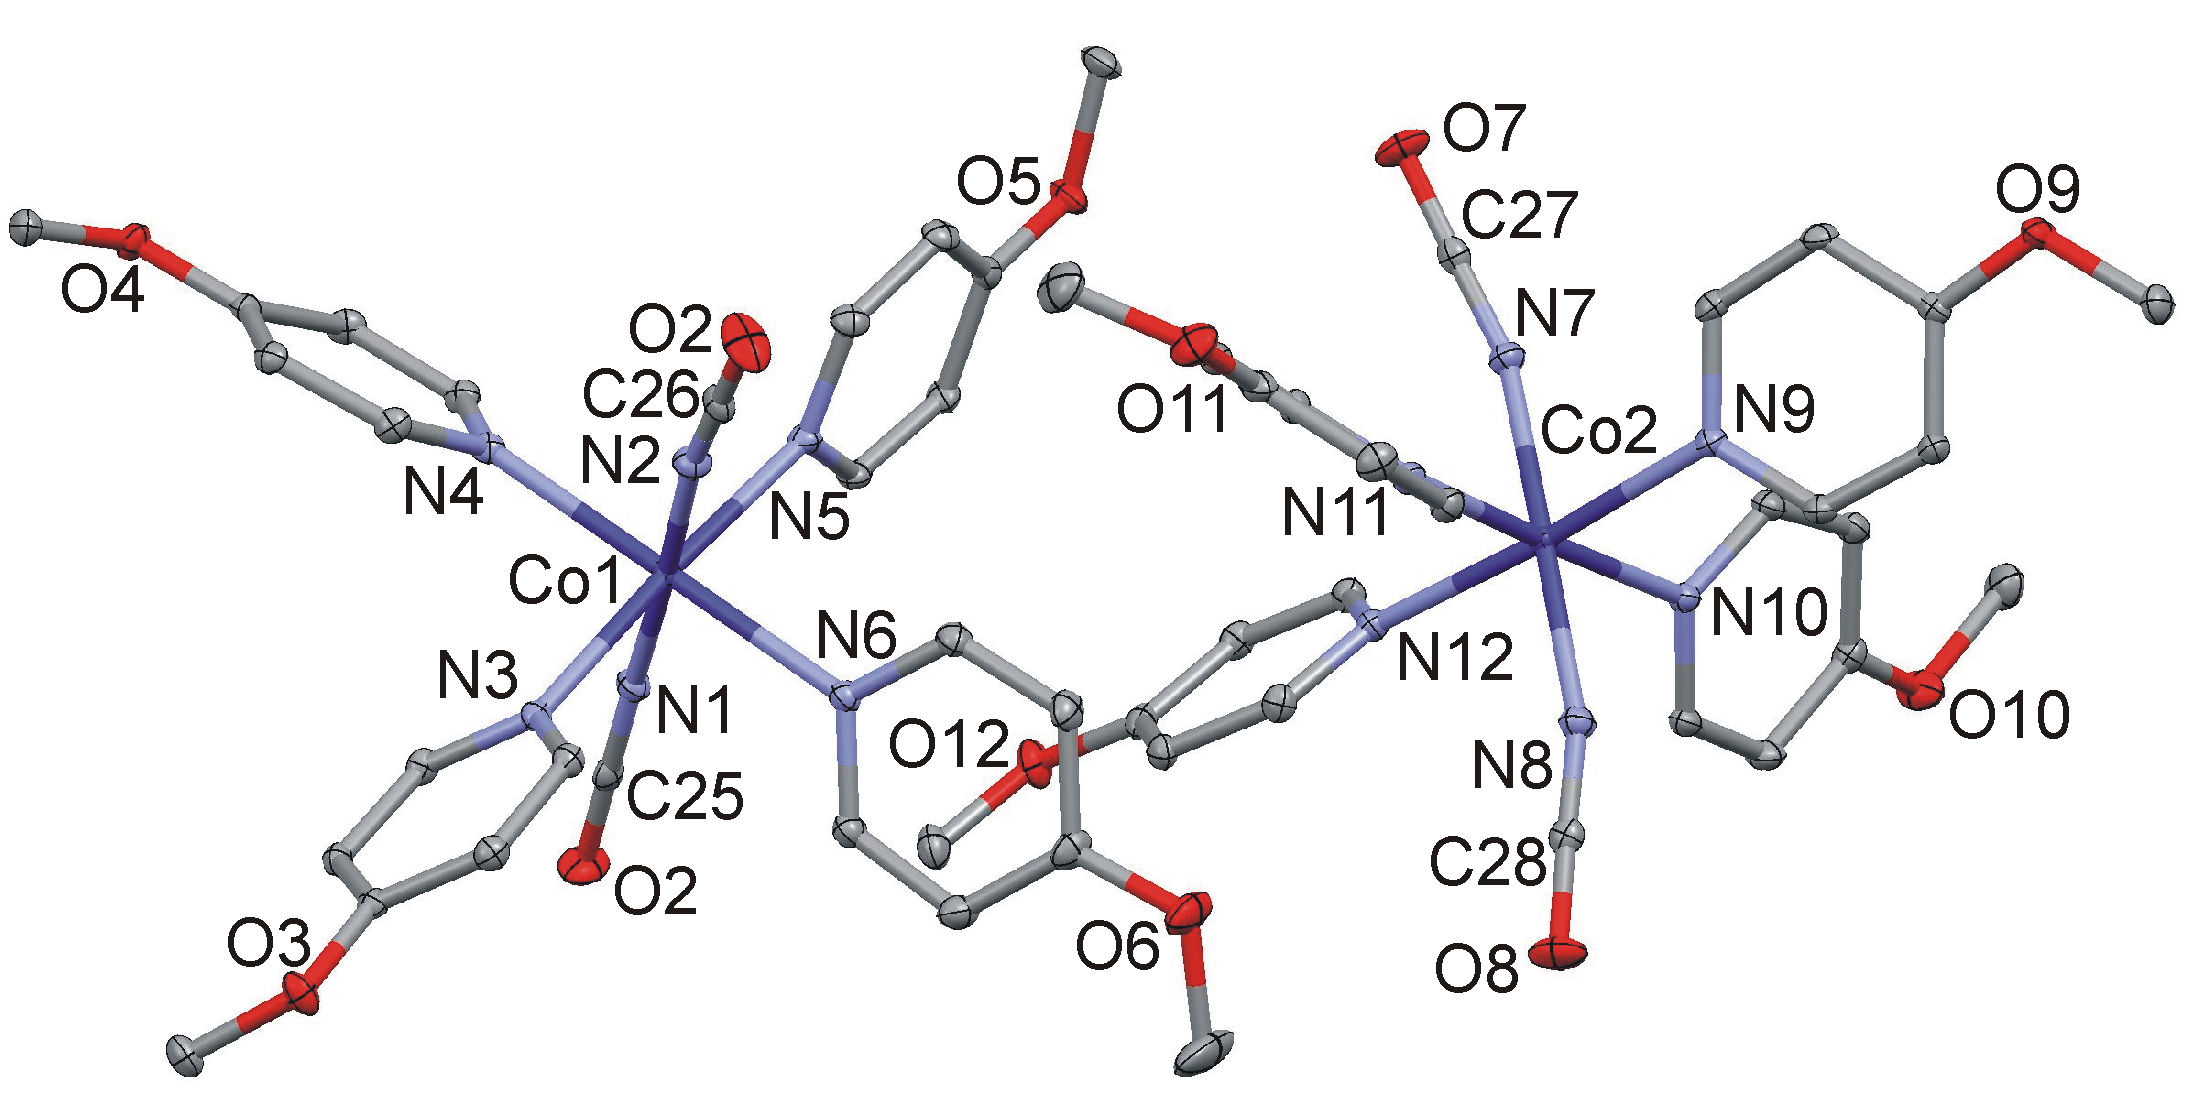
\includegraphics[width=1\textwidth]{figures/coomop_FIGm11.png}
\caption[Perspective view of \ce{[Co(OCN)_2(4-MeOpy)_4]}]{Perspective view of \ce{[Co(OCN)_2(4-MeOpy)_4]} with the atom numbering scheme.}
\label{fig:CoO4MOP_pv}
\vspace{\floatsep}
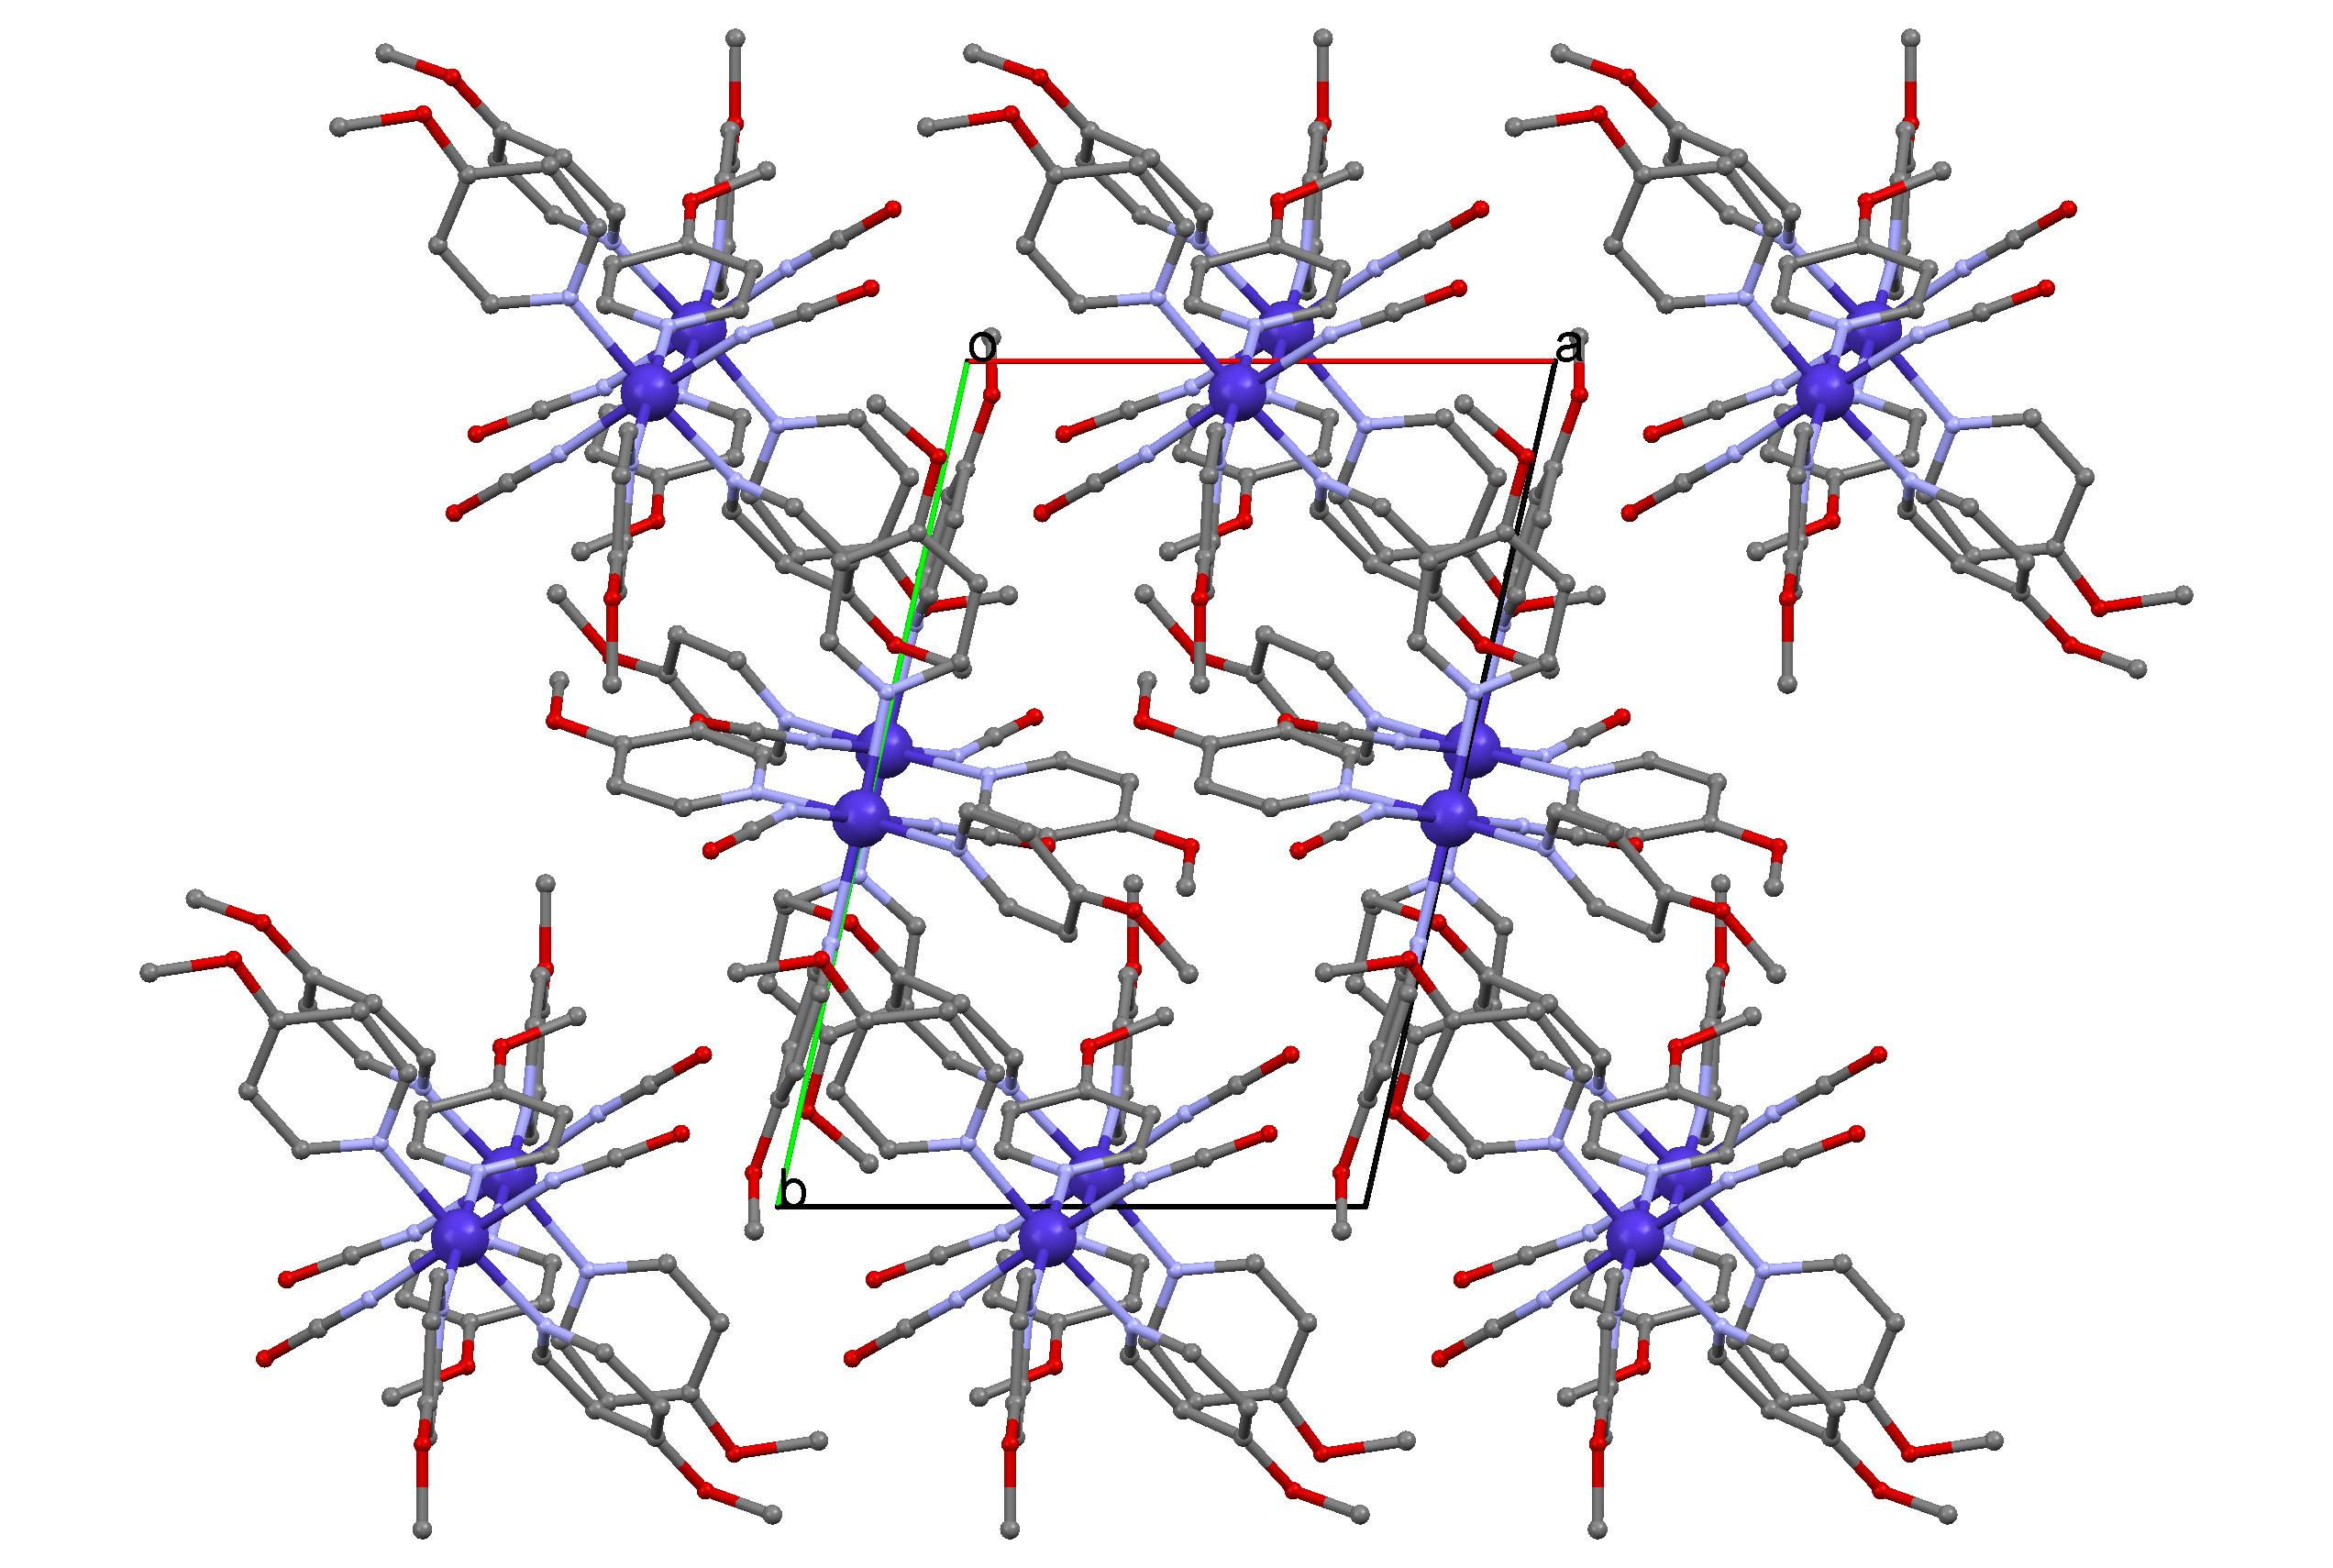
\includegraphics[width=1\textwidth]{figures/coomop_CC.png}
\caption{Packing view  of \ce{[Co(OCN)_2(4-MeOpy)_4]}.}
\label{fig:CoO4MOP_packv}
\end{figure}


\renewcommand{\arraystretch}{1.5}
\begin{table}
\centering
\captionabove{Crystallographic data and processing parameter of \ce{[Co(OCN)_2(4-MeOpy)_4]}}
\begin{tabular}{ | l |  l | }
\hline
Empirical formula & \ce{C_{26}H_{28}CoN_{6}O_{6}}\\
\hline
Formula mass & 579.47\\
\hline
System & triclinic\\
\hline
Space group & P-1\\
\hline
a ({\AA}) & 10.1989(12)\\
\hline
b ({\AA}) & 15.3641(18)\\
\hline
c ({\AA}) & 19.234(3)\\
\hline
$\alpha$ ($^\circ$) & 107.209(6)\\
\hline
$\beta$ ($^\circ$) & 102.632(7)\\
\hline
$\gamma$ ($^\circ$) & 98.012(5)\\
\hline
V (\AA$^{3}) $  & 2741.1(6)\\
\hline
Z & 4\\
\hline
T (K) & 100(2)\\
\hline
$\mu$ (mm$^{-1}$) & 0.677\\
\hline
 D$_{calc}$ (Mg/m$^{3}$) & 1.404\\
\hline
Crystal size (mm) & 0.23 x 0.18 x 0.12\\
\hline
$\theta$ max ($^\circ$) & 28.00\\
\hline
Data collected & 168102\\
\hline
Unique refl./ R$_{int}$ & 13238 / 0.0843\\
\hline
Parameters & 711\\
\hline
Goodness-of-Fit on F$^{2}$ & 0.994\\
\hline
R1 / wR2 (all data) & 0.0374 /0.0808\\
\hline
Residual extrema (e/\AA$^{3}$) & 0.35 /-1.49\\
\hline
\end{tabular}

\label{ptbl:CoO4MOP}

\end{table}


\section{\ce{[Cd(dca)_2(4-methoxypyridine)_2]_n}}
\subsection{Synthesis}
0.52 g \ce{CdSO_4* 8/3 H_2O} (2 mmol), 0.36 g Na-dca (4 mmol) and 0.44 g 4-methoxypyridine (4 mmol) were dissolved in 40 mL distill. \ce{H2O}. The mixture was stirred for 140 minutes (at 70$^\circ$C). After the removal of solid compounds, the colourless solution was stirred at the same temperature for 20 minutes. Thereafter the solution was allowed to cool down to RT. After one day white crystals were obtained. Anal. Calculated for \ce{C_{16}H_{14}CdN_{8}O_{2}} (462.76 g/mol) : 41.53\% C; 3.05\% H; 24.21\% N; Found: 41.55 \% C; 3.11\% H; 24.25 \% N; IR (ATR, cm$^{-1}$): 2295 (m), 2227 (m), 2171 (s), 1607 (s), 1566 (m), 1434 (s), 1348 (s), 1302 (s), 1206 (s), 1027 (vs), 933 (w), 813 (s), 711 (w), 675 (m), 569 (w), 521 (s), 461 (m)

\begin{figure}[htpb!]
\centering
\includegraphics[width=1\textwidth]{figures/CdD4MOP-IR_1.pdf}
\caption{IR spectrum of \ce{[Cd(dca)_2(4-MeOpy)_2]_n}}
\end{figure}


\newpage
\subsection{Structural characterization}
 Selected bond parameters of \ce{[Cd(dca)_2(4-MeOpy)_2]_n} are summarized in table \ref{batab:CdD4MOP}, A perspective view of a section of the polymeric chain is given in fig. \ref{fig:CdD4MOP_pv} and a packing view in fig. \ref{fig:CdD4MOP_packv}.  The Co(1) center (located on an inversion center) is coordinated by a pyridine N donor atom for each of two 4-methoxypyridine molecules in trans configuration. Four N atoms of dicyanamide anions act in the bis-$\mu$(1,5)-bridging mode to generate polymeric chains of polyhedra. These atomes are oriented along the b-axis of the triclinic unit cell. The \ce{CdN_6} polyhedron forms an almost regular octahedron, with Cd-N bond distances varying from 2.302(3) to 2.344(4) \AA, and maximum deviation 3.34$^\circ$ of the N-Cd-N bond angles from 90 or 180$^\circ$. The dicyanamide bridges have the following bond parameters: Cd-N-C: 161.7(4) and 155.7(4)$^\circ$; N-C-N: 174.1(5) and 176.0(5)$^\circ$; C-N-C: 118.9(3)$^\circ$; C-N(nitril) 1.150(6) and 1.159(6) \AA; C-N(amide): 1.313(6) and 1.313(6) \AA. The intra-chain Cd\ce{***}Cd distance of 7.5491(9)\AA  is longer than the shortest inter-chain metal\ce{***}metal separation of 7.1028(8) \AA. 

\renewcommand{\arraystretch}{1.5}
\begin{table}[htpb!]
\centering
\captionabove{Selected bond lengths (\AA) and angles ($^\circ$) for \ce{[Cd(dca)_2(4-MeOpy)_2]_n}; Symmetry codes: (a) 2-x,2-y, -z; (b) 2-x, 1-y, -z; (c) x, 1+y, z; (d) x, -1+y, z; (e) 2-x, 3-y, -z; (f) 2-x, -y, -z.}
\begin{tabular}{|l|l|l|l|}
\hline
Cd(1)-N(1a) & 2.302(3) & Cd(1)-N(4b) & 2.344(4)\\
\hline
Cd(1)-N(2a) & 2.342(4) & N(3)-C(7) & 1.313(6)\\
\hline
N(2)-C(7) & 1.150(6) & N(3)-C(8) & 1.313(6)\\
\hline
N(4)-C(8) & 1.159(6) &  & \\
\hline
\hline
N(1)-Cd(1)-N(2a) & 91.32(13) & N(1)-Cd(1)-N(4b) & 90.58(13)\\
\hline
N(4c)-Cd(1)-N(2a) & 93.34(11) & N(2)-Cd(1)-N(2a) & 180.0\\
\hline
Cd(1)-N(2)-C(7) & 161.7(4) & N(2)-C(7)-N(3) & 174.1(5)\\
\hline
Cd(1b)-N(4)-C(8) & 155.7(4) & N(4)-C(8)-N(3) & 176.0(5)\\
\hline
C(7)-N(3)-C(8) & 118.9(3) &  & \\
\hline
\end{tabular}

\label{batab:CdD4MOP}
\end{table}

\begin{figure}[!htpb]
\centering
\includegraphics[width=1\textwidth]{figures/cddca4mop_FIGm11.png}
\caption[Perspective view of \ce{[Cd(dca)_2(4-MeOpy)_2]_n}]{Perspective view of a section of the polymeric chain of  \ce{[Cd(dca)_2(4-MeOpy)_2]_n} together with the atom numbering scheme. Symmetry codes: (a) 2-x,2-y,-z; (b) 2-x,1-y,-z; (c) x,1+y,z; (d) x,-1+y,z; (e) 2-x,3-y,-z; (f) 2-x,-y,-z.}
\label{fig:CdD4MOP_pv}
\vspace{\floatsep}
\includegraphics[width=1\textwidth]{figures/cddca4mop_CB.png}
\caption{Packing plot of \ce{[Cd(dca)_2(4-MeOpy)_2]_n}.}
\label{fig:CdD4MOP_packv}
\end{figure}




\begin{table}
\centering
\captionabove{Crystallographic data and processing parameter of \ce{[Cd(dca)_2(4-MeOpy)_2]_n}}
\begin{tabular}{ | l |  l | }
\hline
Empirical formula & \ce{C_{16}H_{14}CdN_{8}O_{2}}\\
\hline
Formula mass & 462.76\\
\hline
System & triclinic\\
\hline
Space group & P-1\\
\hline
a ({\AA}) & 7.1028(8)\\
\hline
b ({\AA}) & 7.5491(8)\\
\hline
c ({\AA}) & 9.8206(11)\\
\hline
$\alpha$ ($^\circ$) & 71.234(5)\\
\hline
$\beta$ ($^\circ$) & 70.587(5)\\
\hline
$\gamma$ ($^\circ$) & 85.267(5)\\
\hline
V (\AA$^{3}) $  & 470.06(9)\\
\hline
Z & 1\\
\hline
T (K) & 100(2)\\
\hline
$\mu$ (mm$^{-1}$) & 1.190\\
\hline
 D$_{calc}$ (Mg/m$^{3}$) & 1.635\\
\hline
Crystal size (mm) & 0.22 x 0.14 x 0.09\\
\hline
$\theta$ max ($^\circ$) & 27.00\\
\hline
Data collected & 2003\\
\hline
Unique refl./ R$_{int}$ & 2003 / ----\\
\hline
Parameters & 126\\
\hline
Goodness-of-Fit on F$^{2}$ & 1.040\\
\hline
R1 / wR2 (all data) & 0.0383 /0.0836\\
\hline
Residual extrema (e/\AA$^{3}$) & 0.95 /-1.05\\
\hline
\end{tabular}

\label{ptab:CdD4MOP}


\end{table}





\section{\ce{[Cu(dca)_2(4-methoxypyridine)_2]_n}}
\subsection{Synthesis}
2 mmol \ce{Cu(NO_3)_2 * 3 H_2O} (0.48 g), 4 mmol  Na-dicyanamide (0.36 g) and  4 mmol 4-methoxy-pyridine (0.44 g) were dissolved in 45 mL distilled \ce{H_2O}. After stirring for 1 hour at 70$^\circ$C, the mixture was filtered. Then the blue solution was placed in the drying oven ($70^\circ$C) overnight and  cooled down to RT on the next day. A few hours later plate-like  blue crystals were obtained.
Anal. Calculated for \ce{C_{16}H_{14}CuN_{8}O_{2}} (413.90 g/mol) : 46.43\% C; 3.41\% H; 27.07\% N;
Found: 46.45 \% C; 3.44\% H; 27.03 \% N;
IR (ATR, cm$^{-1}$):  2292 (s), 2235 (s), 2169 (s), 1614 (s), 1566 (m), 1510 (m), 1437 (m), 1348 (m), 1303 (s), 1202 (m), 1031 (s), 928 (w), 817 (s), 731 (w), 670 (m), 517 (s)


\begin{figure}[h!]
\centering
\includegraphics[scale=0.9, width=1\textwidth]{figures/CuD4MOP-IR.pdf}
\caption{IR spectrum of \ce{[Cu(dca)_2(4-MeOpy)_2]_n}}
\end{figure}

\subsection{Structural characterization}

A section of the polymeric chain of \ce{[Cu(dca)_2(4-MeOpy)_2]_n} is depicted in a perspective and a packing view in fig. \ref{fig:CuD4MOP_pv} and fig. \ref{fig:CuD4MOP_packv}. Table \ref{batab:CuD4MOP} shows the bond parameters which have been selected. Two 4-methoxypyridine molecules bind to Cu(1), which is placed on an inversion center. This central metal atom is also connected via the N atoms of four dicyanamide anions. The latter are acting as bis-$\mu$(1,5)-bridging ligands, generating a chain of polyhedra along the b axis of the triclinic unit cell. The \ce{CuN_6} chromophore has an elongated square bipyramidal geometry, with short Cu(1)-N(1) and Cu(1)-N(2) bond distances of 2.0219(9) and 2.0038(10) \AA, respectively, and semi-coordinative Cu(1)-N(4b,c) bond distances of 2.4556(10) \AA. The asymmetric dicyanamide bridges have the following bond parameters: Cu-N-C: 169.61(9) and 148.10(9)$^\circ$; N-C-N: 174.47(12) and 175.12(12)$^\circ$; C-N-C: 119.26(10)$^\circ$; C-N(nitril) 1.1555(15) and 1.1562(15) \AA; C-N(amide): 1.3158(15) and 1.3019(15) \AA. The intra-chain Cu\ce{***}Cu distance of 7.3799(4) \AA  is longer than the shortest inter-chain metal\ce{***}metal separation of 7.0318(4) \AA. 

\renewcommand{\arraystretch}{1.5}
\begin{table}[htpb!]
\centering
\captionabove{Selected bond lengths (\AA) and angles ($^\circ$) for \ce{[Cu(dca)_2(4-MeOpy)_2]_n}; Symmetry codes: (a) -x, -y, 2-z; (b) -x, 1-y, 2-z; (c) x, -1+y, z; (d) x, 1+y, z; (e) -x, -1-y; 2-z; (f) -x, 2-y, 2-z.}
\begin{tabular}{|l|l|l|l|}
\hline
Cu(1)-N(1a) & 2.0219(9) & Cu(1)-N(4b) & 2.4556(10)\\
\hline
Cu(1)-N(2a) & 2.0038(10)& N(3)-C(7) & 1.3158(15)\\
\hline
N(2)-C(7) & 1.1555(15) & N(3)-C(8) & 1.3019(15)\\
\hline
N(4)-C(8) & 1.1562(15) &  & \\
\hline
\hline
N(2)-Cu(1)-N(1a) & 90.33(4) & N(1)-Cu(1)-N(4b) & 90.31(4)\\
\hline
N(4c)-Cu(1)-N(2a) & 92.10(4) & N(2)-Cu(1)-N(2a) & 180.0\\
\hline
Cu(1)-N(2)-C(7) & 169.61(9) & N(2)-C(7)-N(3) & 174.47(12)\\
\hline
Cu(1b)-N(4)-C(8)& 148.10(9) &N(4)-C(8)-N(3) & 175.12(12)\\
\hline
C(7)-N(3)-C(8)& 119.26(10) & &\\
\hline
\end{tabular}
\label{batab:CuD4MOP}
\end{table}


\begin{figure}[!htpb]
\centering
\includegraphics[width=1\textwidth]{figures/cudmop_FIGm11-1.png}
\caption[Perspective view of \ce{[Cu(dca)_2(4-MeOpy)_2]_n}] {Perspective view of a section of the polymeric chain of \ce{[Cu(dca)_2(4-MeOpy)_2]_n} together with the atom numbering scheme. Symmetry codes: (a) -x,-y,2-z; (b) -x,1-y,2-z; (c) x,-1+y,z; (d) x,1+y,z; (e) -x,-1-y,2-z; (f) –x,2-y,2-z.}
\label{fig:CuD4MOP_pv}
\vspace{\floatsep}
\includegraphics[width=1\textwidth]{figures/cudmop_CB-1.png}
\caption{Packing plot  of \ce{[Cu(dca)_2(4-MeOpy)_2]_n}.}
\label{fig:CuD4MOP_packv}
\end{figure}


\begin{table}
\centering
\captionabove{Crystallographic data and processing parameter of \ce{[Cu(dca)_2(4-MeOpy)_2]n}}
\begin{tabular}{ | l |  l | }
\hline
Empirical formula & \ce{C_{16}H_{14}CuN_{8}O_{2}}\\
\hline
Formula mass & 413.90\\
\hline
System & triclinic\\
\hline
Space group & P-1\\
\hline
a ({\AA}) & 7.0318(3)\\
\hline
b ({\AA}) & 7.3799(3)\\
\hline
c ({\AA}) & 9.7467(5)\\
\hline
$\alpha$ ($^\circ$) & 69.519(2)\\
\hline
$\beta$ ($^\circ$) & 70.257(2)\\
\hline
$\gamma$ ($^\circ$) & 85.367(2)\\
\hline
V (\AA$^{3}) $  & 445.57(4)\\
\hline
Z & 1\\
\hline
T (K) & 100(2)\\
\hline
$\mu$ (mm$^{-1}$) & 1.256\\
\hline
 D$_{calc}$ (Mg/m$^{3}$) & 1.543\\
\hline
Crystal size (mm) & 0.25 x 0.15 x 0.10\\
\hline
$\theta$ max ($^\circ$) & 29.63\\
\hline
Data collected & 24435\\
\hline
Unique refl./ R$_{int}$ & 2514 / 0.0361\\
\hline
Parameters & 125\\
\hline
Goodness-of-Fit on F$^{2}$ & 1.121\\
\hline
R1 / wR2 (all data) & 0.0203 /0.0578\\
\hline
Residual extrema (e/\AA$^{3}$) & 0.42 /-0.43\\
\hline
\end{tabular}

\label{ptab:CuD4MOP}

\end{table}




\section{\ce{[Zn(dca)_2(4-methoxypyridine)_2]_n}}
\subsection{Synthesis}
20 mL distilled \ce{H_2O} were used as a solvent for 0.30 g \ce{Zn(NO_3)_2 * 6 H_2O} (1 mmol), 0.18 g Na-dicyanamide (2 mmol) and 0.22 g 4-methoxypyridine (2 mmol). The solution was heated up to $80^\circ$C  and stirred for 1 hour. After filtration, the clear  solution was put in the drying oven at $80^\circ$C overnight and then slowly cooled down to 20$^\circ$ in a waterbath. A few hours later white crystals were obtained.
Anal. Calculated for \ce{C_{16}H_{14}N_8O_2Zn} (415.74 g/mol) : 46.28\% C; 3.40\% H; 26.98\% N;
Found: 46.23 \% C; 3.43\% H; 26.98 \% N;
 IR (ATR, cm$^{-1}$): 2294 (m), 2233 (m), 2170 (s), 1922 (w), 1667 (w), 1611 (s), 1566 (s), 1512 (s), 1433 (s), 1345 (s), 1304 (vs), 1206 (s), 1056 (m), 1008 (s), 936 (m), 830 (s), 814 (s), 673 (m), 571 (w), 526 (s), 463 (m)

\begin{figure}[h!]
\centering
\includegraphics[width=1\textwidth]{figures/ZnD4MOP-IR.pdf}
\caption{IR-Spectrum of \ce{[Zn(dca)_2(4-MeOpy)_2]_n}}
\end{figure}

\subsection{Structural characterization}


The selected bond parameters of \ce{[Zn(dca)_2(4-MeOpy)_2]_n} are summarized in table \ref{batab:ZnD4MOP}. Its crystal structure is displayed in fig. \ref{fig:ZnD4MOP_pv} (perspective view) and fig. \ref{fig:ZnD4MOP_packv} (packing view).  Zn(1) is situated on an inversion center and connected to six ligands: four of them are dicyanamide anions which act in bis-$\mu$(1,5)-bridging mode, forming a polymeric chain along the axis of the triclinic cell. The others are 4-MOP molecules in trans configuration. The \ce{ZnN_6} polyhedron forms an almost regular octahedron, with Zn-N bond distances varying from 2.1288(15) to 2.1733(19) \AA, and a maximum deviation of 0.89$^\circ$ of the N-Zn-N bond angles from 90 or 180$^\circ$. The dicyanamide bridges have the following bond parameters: Zn-N-C: 162.01(18) and 159.00(19)$^\circ$; N-C-N: 174.9(2) and 175.6(2)$^\circ$; C-N-C: 118.38(17)$^\circ$; C-N(nitril) 1.154(3) and 1.158(3) \AA; C-N(amide): 1.310(3) and 1.309(3) \AA. The intra-chain Zn\ce{***}Zn distance of 7.3706(4) \AA \ \ is longer than the shortest inter-chain metal\ce{***}metal separation of 7.0620(4) \AA. 

\renewcommand{\arraystretch}{1.5}

\begin{table}[htpb!]
\centering
\captionabove{Selected bond lengths (\AA) and angles ($^\circ$) for \ce{[Zn(dca)_2(4-MeOpy)_2]_n}; Symmetry codes: (a) 2-x, 2-y, -z; (b) 2-x, 1-y, -z; (c) x, 1+y, z; (d) x, -1+y, z; (e) 2-x, 3-y; -z; (f) 2-x, -y, -z.}
\begin{tabular}{|l|l|l|l|}
\hline
Zn(1)-N(1a) & 2.1288(15) & Zn(1)-N(4b) & 2.1733(19)\\
\hline
Zn(1)-N(2a) & 2.1710(19)& N(3)-C(7) & 1.310(3)\\
\hline
N(2)-C(7) & 1.154(3) & N(3)-C(8) & 1.309(3)\\
\hline
N(4)-C(8) & 1.158(3) &  & \\
\hline
\hline
N(1)-Zn(1)-N(2a) & 90.59(7) & N(1a)-Zn(1)-N(4b) & 90.28(7)\\
\hline
N(4c)-Zn(1)-N(2a) & 90.89(6) & N(2)-Zn(1)-N(2a) & 180.0\\
\hline
Zn(1)-N(2)-C(7) & 162.01(18) & N(2)-C(7)-N(3) & 174.9(2)\\
\hline
Zn(1b)-N(4)-C(8)& 159.00(19) &N(4)-C(8)-N(3) & 175.6(2)\\
\hline
C(7)-N(3)-C(8)& 118.38(17) & &\\
\hline
\end{tabular}
\label{batab:ZnD4MOP}
\end{table}


\begin{figure}[!htpb]
\centering
\includegraphics[width=1\textwidth]{figures/ZnD_4MOP_FIGm11.png}
\caption[Perspective view of \ce{[Zn(dca)_2(4-MeOpy)_2]_n}]{Perspective view of a section of the polymeric chain of \ce{[Zn(dca)_2(4-MeOpy)_2]_n} together with the atom numbering scheme. Symmetry codes: (a) 2-x,2-y,-z; (b) 2-x,1-y,-z; (c) x,1+y,z; (d) x,-1+y,z; (e) 2-x,3-y,-z; (f) 2-x,-y,-z.}
\label{fig:ZnD4MOP_pv}
\vspace{\floatsep}
\includegraphics[width=1\textwidth]{figures/znd_4mop_CB.png}
\caption{Packing plot  of \ce{[Zn(dca)_2(4-MeOpy)_2]_n}.}
\label{fig:ZnD4MOP_packv}
\end{figure}



\begin{table}
\centering
\captionabove{Crystallographic data and processing parameter of \ce{[Zn(dca)_2(4-MeOpy)_2]_n}.}
\begin{tabular}{ | l |  l | }
\hline
Empirical formula & \ce{C_{16}H_{14}N_{8}O_{2}Zn}\\
\hline
Formula mass & 415.74\\
\hline
System & triclinic\\
\hline
Space group & P-1\\
\hline
a ({\AA}) & 7.0620(4)\\
\hline
b ({\AA}) & 7.3706(4)\\
\hline
c ({\AA}) & 9.8134(5)\\
\hline
$\alpha$ ($^\circ$) & 69.847(2)\\
\hline
$\beta$ ($^\circ$) & 71.759(3)\\
\hline
$\gamma$ ($^\circ$) & 86.183(3)\\
\hline
V (\AA$^{3}) $  & 454.94(4)\\
\hline
Z & 1\\
\hline
T (K) & 100(2)\\
\hline
$\mu$ (mm$^{-1}$) & 1.379\\
\hline
 D$_{calc}$ (Mg/m$^{3}$) & 1.518\\
\hline
Crystal size (mm) & 0.26 x 0.21 x 0.12\\
\hline
$\theta$ max ($^\circ$) & 28.00\\
\hline
Data collected & 2188\\
\hline
Unique refl./ R$_{int}$ & 2188 / ----\\
\hline
Parameters & 126\\
\hline
Goodness-of-Fit on F$^{2}$ & 1.148\\
\hline
R1 / wR2 (all data) & 0.0282 /0.0798\\
\hline
Residual extrema (e/\AA$^{3}$) & 0.40 /-0.40\\
\hline
\end{tabular}

\label{ptab:ZnD4MOP}

\end{table}


 


\section{\ce{[Co(SCN)_2(4-methoxypyridine)_4]}}
\subsection{Synthesis}
0.58 g \ce{Co(NO_3)_2* 6 H_2O} (2 mmol), 0.38 g KSCN (4 mmol) and 0.87 g 4-methoxy-pyridine (8 mmol) were dissolved in 40 mL distilled \ce{H_2O}. The solution was heated up to $70^\circ$C  and stirred for 1 hour. After filtration the clear pink solution was placed in the drying oven ($70^\circ$C) overnight and then cooled down to RT. After a few hours pink crystals were obtained.
Anal. Calculated for \ce{C_{26}H_{28}CoN_{6}O_{4}S_{2}} (611,59 g/mol): 51.06\% C; 4.61\% H; 13.74\% N; 10.49 \% S;
Found: 50.94 \% C; 4.65\% H; 13.80 \% N; 10.30\% S;
IR (ATR, cm$^{-1}$): 2061 (s), 1608 (s), 1567 (s), 1508 (s), 1493 (s), 1460 (w), 1426 (m), 1293 (s), 1205 (s), 1024 (vs), 822 (s), 659 (w), 540 (s), 458 (m)

\begin{figure}[h!]
\centering
\includegraphics[width=1\textwidth]{figures/CoR4MOP-IR.pdf}
\caption{IR spectrum of \ce{[Co(SCN)_2(4-MeOpy)_4]}}
\end{figure}





\subsection{Structural characterization}

The crystal structure of \ce{[Co(SCN)_2(4-MeOpy)_4]}) consists of mononuclear and neutral Co(II) complexes. A perspective view is shown in fig. \ref{fig:CoR4MOP_pv}, a packing view in fig \ref{fig:CoR4MOP_packv} and selected bond parameters are summarized in table \ref{batlb:CoR4MOP}. Co(1) is six-coordinated by N atoms of two terminal isothiocyanato anions, further by N donor atoms of four neutral 4-methoxypyridine molecules. The \ce{CoN6} chromophore may be described as a slighly distorted octahedron with trans-arrangement of the isothiocyanato ligands. The Co-N bond lengths range from 2.089(5) to 2.195(5) \AA, and the transoid N-Co-N bond angles within the \ce{CoN6} octahedra vary from 175.08(17) to 178.96(18)$^\circ$. The bond parameters of the terminal isothiocyanato anions are: Co-N-C: 153.9(4) and 163.4(5)$^\circ$, N-C-S: 178.0(5) and 179.4(6)$^\circ$, N-C: 1.160(7) and 1.167(7) \AA, C-S: 1.637(5) and 1.628(6) \AA.The shortest metal-metal separation is 9.1969(19) \AA. 

\begin{table}[htpb!]
\centering
\captionabove{Selected bond lengths (\AA) and angles ($^\circ$) for \ce{[Co(SCN)_2(4-MeOpy)_4]}}
\begin{tabular}{|l|l|l|l|}
\hline
Co(1)-N(1) & 2.096(5) & Co(1)-N(4) & 2.195(5)\\
\hline
Co(1)-N(2) & 2.089(5) & Co(1)-N(5) & 2.136(5)\\
\hline
Co(1)-N(3) & 2.174(5) & Co(1)-N(6) & 2.155(5)\\
\hline
N(1)-C(1) & 1.160(7) & C(1)-S(1) & 1.637(5)\\
\hline
N(2)-C(2) & 1.167(7) & C(2)-S(2) & 1.628(6)\\
\hline
\hline
N(1)-Co(1)-N(2) & 178.96(18) & N(3)-Co(1)-N(5) & 175.08(17)\\
\hline
N(4)-Co(1)-N(6) & 1.178.44(17) & Co(1)-N(2)-C(2) & 153.9(4)\\
\hline
Co(1)-N(1)-C(1) & 163.4(5) & N(2)-C(2)-S(2) & 178.0(5)\\
\hline
N(1)-C(1)-S(1) & 179.4(6) & & \\
\hline
\end{tabular}
\label{batlb:CoR4MOP}
\end{table}



\begin{figure}[!htpb]
\centering
\includegraphics[width=1\textwidth]{figures/cormop_FIGm11.png}
\caption[Perspective view of \ce{[Co(SCN)_2(4-MeOpy)_4]}]{Perspective view of \ce{[Co(SCN)_2(4-MeOpy)_4]} with the atom numbering scheme.}
\label{fig:CoR4MOP_pv}
\vspace{\floatsep}
\includegraphics[width=1\textwidth]{figures/cormop_CB.png}
\caption{Packing view  of \ce{[Co(SCN)_2(4-MeOpy)_4]}.}
\label{fig:CoR4MOP_packv}
\end{figure}


\renewcommand{\arraystretch}{1.5}
\begin{table}
\centering
\captionabove{Crystallographic data and processing parameter of \ce{[Co(SCN)_2(4-MeOpy)_4]}}
\begin{tabular}{ | l |  l | }
\hline
Empirical formula & \ce{C_{26}H_{28}CoN_{6}O_{4}S_{2}}\\
\hline
Formula mass & 611.59\\
\hline
System & orthorhombic\\
\hline
Space group & Pbca\\
\hline
a ({\AA}) & 10.1815(17)\\
\hline
b ({\AA}) & 16.574(3)\\
\hline
c ({\AA}) & 34.268(6)\\
\hline
$\alpha$ ($^\circ$) & 90\\
\hline
$\beta$ ($^\circ$) & 90\\
\hline
$\gamma$ ($^\circ$) & 90\\
\hline
V (\AA$^{3}) $  & 5782.6(17)\\
\hline
Z & 8\\
\hline
T (K) & 100(2)\\
\hline
$\mu$ (mm$^{-1}$) & 0.780\\
\hline
 D$_{calc}$ (Mg/m$^{3}$) & 1.405\\
\hline
Crystal size (mm) & 0.19 x 0.16 x 0.09\\
\hline
$\theta$ max ($^\circ$) & 25.50\\
\hline
Data collected & 33321\\
\hline
Unique refl./ R$_{int}$ & 5372 / 0.1050\\
\hline
Parameters & 356\\
\hline
Goodness-of-Fit on F$^{2}$ & 1.154\\
\hline
R1 / wR2 (all data) & 0.0763 /0.1570\\
\hline
Residual extrema (e/\AA$^{3}$) & 0.64 /-0.85\\
\hline
\end{tabular}

\label{ptab:CoR4MOP}

\end{table}



\section{\ce{[Cu(SCN)_2(4-methoxypyridine)_2]_n}}
\subsection{Synthesis}
0.48 g \ce{Cu(NO_3)_2 * 3 H_2O} (2 mmol), 0.39 g KSCN (4 mmol) and 0.44 g 4-methoxy-pyridine (4 mmol) were mixed with 40 mL distilled \ce{H_{2}O}. Stirring was conducted for 2 hours and 30 minutes at 60$^\circ$C. After filtration the green solution was stirred again for 50 minutes at the same temperature and then cooled down to RT. Over the course of 24 hours green crystals precipitated.
Anal. Calculated for \ce{C_{14}H_{14}CuN_{4}O_{2}S_{2}} (397.96 g/mol) : 42.25\% C; 3.55\% H; 14.08\% N; 16.11\% S;
Found: 41.84 \% C; 3.51\% H; 14.14 \% N; 15.69\% S;
IR (ATR, cm$^{-1}$): 2086 (s), 2072 (s), 1614 (s), 1566 (s), 1512 (s), 1434 (s), 1299 (s), 1205 (s), 1059 (m), 1030 (s), 1012 (m), 844 (m), 817 (s), 732 (w), 659 (w), 573 (w), 535 (s), 464 (s)


\begin{figure}[h!]
\centering
\includegraphics[scale=0.9, width=1\textwidth]{figures/CuR4MOP-IR.pdf}
\caption{IR spectrum of \ce{[Cu(SCN)_2(4-MeOpy)_2]_n}}
\end{figure}

\subsection{Structural characterization}
A perspective view of \ce{[Cu(SCN)_2(4-MeOpy)_2]_n} is given in fig. \ref{fig:CuR4MOP_pv}. The 2D layer system of the Cu-NCS sublattice is displayed in fig. \ref{fig:CuR4MOP_packv}. Table \ref{batlb:CoR4MOP} lists the chosen bond parameters. The three crystallographically independent Cu(II) metal centers in the structure of Cu(SCN)$_2$(4-Me-O-py)$_2$ are located on inversion centers. Taking into account the semi-coordinative Cu-S bond distances, each Cu(II) is bound to four N and two S atoms, whereas two N belong to two 4-MOPs in trans configuration. The remaining 4 atoms each belong to a isothiocyanate anion. The Cu-N(py) bond distances vary from 2.010(3) to 2.037(2) \AA, the Cu-N(NCS) bond distances vary from 1.953(2) to 1.970(3) \AA, whereas the semi-coordinative Cu-S bond lengths are in the range of 2.930(2) to 3.112(2) \AA. The three NCS-groups behave in a different manner. N(2)-C(2)-S(2) acts as N-terminal ligand only, N(1)-C(1)-S(1) acts as  $\mu$(N,S) ligand, to bridge Cu(1) and Cu(3) centers, N(3)-C(3)-S(3) acts as $\mu$(N,S,S’)-bridging ligand to connect all three different metal centers. The 2D system of Cu(SCN)$_2$(4-Me-O-py)$_2$ may be described as polymeric chains of alternating Cu(1) and Cu(3) polyhedra oriented along the c-axis. These chains are formed via di-$\mu$-(N,S) bridging NCS-anions. This is where the Cu(1) polyhedra are further connected by Cu(2) polyhedra along the b-axis of the triclinic unit cell (Fig. \ref{fig:CuR4MOP_packv}). The N(1)-C(1)-S(1) $\mu$(N,S) bridge has a Cu-N\ce{***}S-Cu torsion angle of +64.1$^\circ$, and the N(3)-C(3)-S(3) $\mu$(N,S,S’)-bridge forms Cu-N\ce{***}S-Cu torsion angles of  -27.1 and -165.7$^\circ$. 

\renewcommand{\arraystretch}{1.5}
\begin{table}[htpb!]
\centering
\captionabove{Selected bond lengths (\AA) and angles ($^\circ$) for \ce{[Cu(SCN)_2(4-MeOpy)_2]_n}. Symmetry codes: (') 1-x, -y, 2-z; (*) 1-x, 1-y, -z; ('') 1-x, 2-y, 1-z. }
\begin{tabular}{|l|l|l|l|}
\hline
Cu(1)-N(1') & 1.953(2) & Cu(1)-N(5') & 2.037(2)\\
\hline
Cu(2)-N(2*) & 1.958(3) & Cu(2)-N(6*) & 2.027(2)\\
\hline
Cu(3)-N(3'') & 1.970(3) & Cu(3)-N(7'') & 2.010(3)\\
\hline
N(1)-C(1) & 1.159(4) & C(1)-S(1) & 1.635(3)\\
\hline
N(2)-C(2) & 1.145(4) & C(2)-S(2) & 1.622(4)\\
\hline
N(3)-C(3) & 1.157(4) & C(3)-S(3) & 1.641(3)\\
\hline
\hline
N(1')-Cu(1)-N(5') & 90.87(10) & N(2*)-Cu(2)-N(6*) & 90.16(10)\\
\hline
N(3)-Cu(3)-N(7'') & 90.02(11) & N(21)-Cu(1)-N(11a) & 91.04(9)\\
\hline
Cu(1)-N(1)-C(1) & 162.3(2) & N(1)-C(1)-S(1) & 179.6(3)\\
\hline
Cu(2)-N(2)-C(2) & 155.0(3) &N(2)-C(2)-S(2) & 179.4(3)\\
\hline
Cu(3)-N(3)-C(3) & 168.3(2) & N(3)-C(3)-S(3) & 178.8(3)\\
\hline
\end{tabular}
\label{batlb:CoR4MOP}
\end{table}



\begin{figure}[htpb!]
\centering
\includegraphics[width=1\textwidth]{figures/curmop_FIGm11.png}
\caption[Perspective view of \ce{[Cu(SCN)_2(4-MeOpy)_2]}]{Perspective view of \ce{[Cu(SCN)_2(4-MeOpy)_2]_n} with the atom numbering scheme. Symmetry codes: (') 1-x, -y, 2-z; (*) 1-x, 1-y, -z; ('') 1-x, 2-y, 1-z.}
\label{fig:CuR4MOP_pv}
\vspace{\floatsep}
\includegraphics[width=1\textwidth]{figures/curmop_2D.png}
\caption{View onto 2D Cu-NCS sub-lattice of \ce{[Cu(SCN)_2(4-MeOpy)_2]_n}.}
\label{fig:CuR4MOP_packv}
\end{figure}




\begin{table}
\centering
\captionabove{Crystallographic data and processing parameter of \ce{[Cu(SCN)_2(4-MeOpy)_2]_n}}
\begin{tabular}{ | l |  l | }
\hline
Empirical formula & \ce{C_{14}H_{14}CuN_{4}O_{2}S_{2}}\\
\hline
Formula mass & 397.96\\
\hline
System & triclinic\\
\hline
Space group & P-1\\
\hline
a ({\AA}) & 10.981(2)\\
\hline
b ({\AA}) & 11.296(2)\\
\hline
c ({\AA}) & 11.531(2)\\
\hline
$\alpha$ ($^\circ$) & 112.524(3)\\
\hline
$\beta$ ($^\circ$) & 99.366(3)\\
\hline
$\gamma$ ($^\circ$) & 98.311(2)\\
\hline
V (\AA$^{3}) $  & 1269.6(4)\\
\hline
Z & 3\\
\hline
T (K) & 100(2)\\
\hline
$\mu$ (mm$^{-1}$) & 1.549\\
\hline
 D$_{calc}$ (Mg/m$^{3}$) & 1.561\\
\hline
Crystal size (mm) & 0.34 x 0.18 x 0.04\\
\hline
$\theta$ max ($^\circ$) & 26.37\\
\hline
Data collected & 10186\\
\hline
Unique refl./ R$_{int}$ & 5122 / 0.0266\\
\hline
Parameters & 384\\
\hline
Goodness-of-Fit on F$^{2}$ & 1.047\\
\hline
R1 / wR2 (all data) & 0.0410 /0.0998\\
\hline
Residual extrema (e/\AA$^{3}$) & 1.23 /-1.29\\
\hline
\end{tabular}

\label{ptab:CuR4MOP}

\end{table}







\chapter{4-hydroxymethylpyridine complexes}
\section{\ce{[Cu(N_3)_2(4-hydroxymethylpyridine)]_n}}
\subsection{Synthesis}
0.48 g \ce{Cu(NO_3)_2*3 H_2O} (2 mmol), 0.26 g sodium azide (4 mmol) and 0.22 g 4-(hydroxymethyl)pyridine (2 mmol) were added to 40 mL distilled water. The solution was heated up for 120 minutes at 70$^\circ$C. After filtration the solution was heated up 50 minutes at 70$^\circ$C and then cooled down to RT. Green needles were obtained after one day.\\
 Anal. Calculated for \ce{C_{6}H_{7}CuN_{7}O} (256.74 g/mol): 28.07\% C; 2.75\% H; 38.19\% N;\\
Found: 28.09 \% C; 2.78\% H; 38.09 \% N;\\
IR (ATR, cm$^{-1}$): 3355 (w),  2025 (vs), 1616 (m), 1562 (w), 1505 (w), 1432 (m), 1289 (m), 1221 (m), 1034 (s), 960 (w), 806 (m), 618 (m), 587 (m), 483 (m)

\newpage
\begin{figure}[htpb!]
\centering
\includegraphics[width=1\textwidth]{figures/CuA4HOMP-IR.pdf}
\caption{IR-Spectrum of \ce{[Cu(N_3)_2(4-HOMepy)]_n}}
\end{figure}

\subsection{Structural characterization}
 Selected bond parameters of \ce{[Cu(N_3)_2(4-HOMepy)]_n} are summarized in table \ref{batab:CuA4HOMP}, a perspective view of a section of the polymeric chain is given in fig. \ref{fig:CuA4HOMP_pv} and a packing view in fig. \ref{fig:CuA4HOMP_packv}. The Cu(1) metal center is penta-coordinated by pyridine N donor atom of a 4-hydroxymethylpyridine molecule and four N atoms of azide groups. The \ce{CuN5} chromophore forms a distorted square pyramid (SP) with a $\tau$-value of 0.24 ($\tau$-values of 1 and 0 refer to ideal geometries of trigonal bipyramid (TBP) and square pyramid (SP), respectively) \cite{addison}. The apical site is occupied by N(23b) [Cu(1)-N(23b) = 2.462(2) \AA]. The basal Cu-N bond distances range from 1.972(2) to 2.005(2) \AA. The azide groups behave differently. Azide groups N(11)-N(12)-N(13) and N(11a)-N(12a)-N(13a) act as di-EO bridges to connect the polyhedra of Cu(1) and Cu(1a) to centrosymmetric dimeric subunits. The bond parameters within their four-membered \ce{Cu2N2} rings are: Cu(1)-N(11)-Cu(1a) = 101.82(10), N(11)-Cu(1)-N(11a) = 78.18(10), Cu(1)-N(11)-N(12) =  128.59(18) and Cu(1a)-N(11)-N(12) = 125.00(18)$^\circ$. The azide group N(21)-N(22)-N(23) act as asymmetrical single EE azido bridge, with N(21) ligated in basal position and N(23) ligated in axial position. Four such single EE azide bridges connect the centrosymmetric dimeric Cu(1)..Cu(1a) subunits to generate double chains of polyhedra oriented along the a-axis of the unit cell. The Cu(1)-N(21)-Cu(1c)-N(23)-N(22) bond angles are 123.98(19) and 110.51(18)$^\circ$, respectively, and the Cu(1)-N(21)..N(23)-Cu(1c) torsion angle is -92.3$^\circ$. The intra-chain Cu(1)..Cu(1a) and Cu(1)..Cu(1c) distances are 3.1042(6) and 5.2153(9) \AA, and the shortest inter-chain metal-metal separation is 7.5484(12) \AA. The bond distances and bond angle of the EO azide bridge are 1.220(3) \AA, 1.139(4) \AA, and 177.8(3)$^\circ$, whereas the corresponding bond parameters for the EE azide bridge are 1.199(3) \AA, 1.161(3) \AA, and 176.9(3)$^\circ$. The 4-hydroxypyridine molecule forms hydrogen bond of  the type O-H\ce{***}N (O(17)-H(91)\ce{***}N(13’)  = 144(6)$^\circ$, O(17)\ce{***}N(13’) = 2.990(6) \AA; symmetry code (‘): 1-x,2-y,1-z).



\renewcommand{\arraystretch}{1.2}
\begin{table}[htpb!]
\centering
\captionabove{Selected bond lengths (\AA) and angles ($^\circ$) for \ce{[Cu(N_3)_2(4-HOMepy)]_n}. Symmetry codes: (a) 2-x, 1-y, 1-z; (b) -1+x, y, z; (c) 2-x, 1-y, 1-z; (d) 1+x, y, z; (e) -x, 1-y, 1-z; (g) -2x, y, z. }
\begin{tabular}{|l|l|l|l|}
\hline
Cu(1)-N(11a) & 2.005(2) & Cu(1)-N(23b) & 2.462(2)\\
\hline
Cu(1)-N(1) & 1.981(2) & Cu(1)-N(11) & 1.995(2)\\
\hline
Cu(1)-N(21) & 1.972(2) & N(11)-N(12) & 1.220(3)\\
\hline
N(12)-N(13) & 1.139(4) & N(21)-N(22) & 1.199(3)\\
\hline
N(22)-N(23) & 1.161(3) &  & \\
\hline
\hline
N(21)-Cu(1)-N(1) & 94.55(9) & N(21)-Cu(1)-N(11) & 159.74(10)\\
\hline
N(11)-Cu(1)-N(1) & 96.01(9) & N(21)-Cu(1)-N(11a) & 91.04(9)\\
\hline
N(11)-Cu(1)-N(11a) & 78.18(10) & N(21)-Cu(1)-N(23b) & 103.39(9)\\
\hline
N(1)-Cu(1)-N(23b) & 93.42(9) & N(11)-Cu(1)-N(23b) & 93.19(9)\\
\hline
N(11a)Cu(1)-N(23b) & 86.84(9) & N(1)-Cu(1)-N(11a) & 174.18(9)\\
\hline
Cu(1)-N(11)-N(12) & 128.5(18) &N(11)-N(12)-N(13) & 177.8(3)\\
\hline
Cu(1)-N(21)-C(22) & 123.98(19) & N(21)-N(22)-N(23) & 176.9(3)\\
\hline
Cu(1a)-N(11)-N(12) & 125.00(18) & Cu(1)-N(11)-Cu(1a) & 101.82(10)\\
\hline
Cu(1c)-N(23)-N(22) & 110.51(18) &  &\\
\hline

\end{tabular}
\label{batab:CuA4HOMP}
\end{table}






\begin{figure}[!htpb]
\centering
\includegraphics[width=0.90\textwidth]{figures/cuahomp_FIGm12.png}
\caption[Perspective view of \ce{[Cu(N_3)_2(4-HOMepy)]_n}]{Perspective view of a section of the polymeric chain of \ce{[Cu(N_3)_2(4-HOMepy)]_n} with the atom numbering scheme. 
Symmetry codes:(a) 2-x,1-y,1-z; (b) 1+x,y,z; (c) -1+x,y,z; (d) 1-x,1-y,1-z; (e) 3-x,1-y,1-z.}
\label{fig:CuA4HOMP_pv}
\vspace{\floatsep}
\includegraphics[width=0.90\textwidth]{figures/cuahomp_CC.png}
\caption{Packing plot of \ce{[Cu(N_3)_2(4-HOMepy)]_n}.}
\label{fig:CuA4HOMP_packv}
\end{figure}


\renewcommand{\arraystretch}{1.5}

\begin{table}
\captionabove{Crystallographic data and processing parameter of \ce{[Cu(N_3)_2(4-HOMepy)]_n}}
\centering
\begin{tabular}{ | l |  l | }
\hline
Empirical formula & \ce{C_{6}H_{7}CuN_{7}O}\\
\hline
Formula mass & 256.74\\
\hline
System & triclinic\\
\hline
Space group & P-1\\
\hline
a ({\AA}) & 5.2153(8)\\
\hline
b ({\AA}) & 9.6409(15)\\
\hline
c ({\AA}) & 9.7206(15)\\
\hline
$\alpha$ ($^\circ$) & 106.898(3)\\
\hline
$\beta$ ($^\circ$) & 97.332(3)\\
\hline
$\gamma$ ($^\circ$) & 94.151(3)\\
\hline
V (\AA$^{3}) $  & 460.73(12)\\
\hline
Z & 2\\
\hline
T (K) & 100(2)\\
\hline
$\mu$ (mm$^{-1}$) & 2.354\\
\hline
 D$_{calc}$ (Mg/m$^{3}$) & 1.851\\
\hline
Crystal size (mm) & 0.10 x 0.15 x 0.02\\
\hline
$\theta$ max ($^\circ$) & 29.99\\
\hline
Data collected & 12368\\
\hline
Unique refl./ R$_{int}$ & 2692 / 0.0207\\
\hline
Parameters & 160\\
\hline
Goodness-of-Fit on F$^{2}$ & 1.369\\
\hline
R1 / wR2 (all data) & 0.0313 /0.0878\\
\hline
Residual extrema (e/\AA$^{3}$) & 0.59 /-0.68\\
\hline
\end{tabular}

\label{ptab:CuA4HOMP}

\end{table}




\section{\ce{[Co(dca)_2(4-hydroxymethylpyridine)_2]_n}}
\subsection{Synthesis}
0.29 g \ce{Co(NO3)2*6 H2O} (1 mmol), 0.18 g sodium dicyanamide (2 mmol) and 0.22 g \ce{4-hydroxymethyl-pyridine} (2 mmol) were dissolved in 20 mL distilled \ce{ H2O}. The solution was heated up to 80$^\circ$C  and stirred for 2 hours and 30 minutes. After filtration the pink  solution was stirred at the same temperature for 40 minutes and then cooled down to RT. After 24 hours pink plate-like crystals were obtained.
Anal. Calculated for \ce{C_{16}H_{14}CoN_{8}O_{2}} (409.28 g/mol) : 46.96\% C; 3.45\% H; 27.38\% N;
Found: 46.76 \% C; 3.44\% H; 27.37 \% N;
IR (ATR, cm$^{-1}$): 3551(w), 3481 (w), 2269 (w), 2245 (m), 2170 (s), 1606 (m), 1564 (w), 1504 (w), 1426 (m), 1293 (s), 1202 (m), 1023 (vs), 799 (m), 607 (w), 533 (s), 493 (m)

\begin{figure}[h!]
\centering
\includegraphics[width=1\textwidth]{figures/CoD4HOMP-IR.pdf}
\caption{IR spectrum of \ce{[Co(dca)_2(4-HOMepy)_2]_n}}
\end{figure}

\newpage


\subsection{Structural characterization}

A packing view  of \ce{[Co(dca)_2(4-HOMepy)_2]_n} is given in fig. \ref{fig:CoD4HOMP_packv} and a perspective view of a section of the polymeric chain  in fig. \ref{fig:CoD4HOMP_pv}. Selected bond parameters are summarized in table \ref{batab:CoD4HOMP}.  The Co(1) center is located on an inversion center. It is coordinated by pyridine N donor atom of two 4-MeOpy molecules in trans configuration and four N atoms of dicyanamide anions (acting in the bis-$\mu$(1,5)-bridging mode) generating polymeric chains of polyhedra. These are oriented along the c-axis of the monoclinic unit cell. The \ce{CoN6} chromophore has an almost regular octahedron, with Co-N bond distances varying from 2.116(4) to 2.126(4) \AA, and N-Co-N bond angles deviating only by 1.16$^\circ$ from the values of ideal octahedral geometry. The dca bridges possess the following bond parameters: Co-N-C: 163.3(4) and 158.5(4)$^\circ$; N-C-N: 177.0(5) and 176.5(
5)$^\circ$; C-N-C: 114.7(4)$^\circ$; C-N(nitril) 1.146(7) and 1.156(7) \AA; C-N(amide): 1.317(7) and 1.326(7) \AA. The intra-chain Co\ce{***}Co distance of 7.213(3) \AA\ \ is longer than the shortest inter-chain metal\ce{***}metal separation of 7.076(3) \AA. Along the a-axis of the unit cell the OH-group of the pyridine derivative ligand forms a hydrogen bond. This bond is  of  the type O-H\ce{***}N and is connected to the central N(3) atom of the adjacent dicyanamide anion (O(1)-H(90)\ce{***}N(3\#1) = 152(7)$^\circ$, O(1)ce{***}N(3\#1) = 2.954(7) \AA; (\#1): 1+x,y,z).



\renewcommand{\arraystretch}{1.2}
\begin{table}[htpb!]
\centering
\captionabove{Selected bond lengths (\AA) and angles ($^\circ$) for \ce{[Co(dca)_2(4-HOMepy)_2]_n}. Symmetry codes: (a) 1-x,1-y,-z; (b) 1-x,1-y,1-z; (c) -1+x,y,z; (d) x,y,1+z; (e) 1-x,1-y,-1-z. }
\begin{tabular}{|l|l|l|l|}
\hline
Co(1)-N(1a) & 2.126(4) & Co(1)-N(4a) & 2.124(5)\\
\hline
Co(1)-N(2a) & 2.116(4) & N(3)-C(7) & 1.317(7)\\
\hline
N(2)-C(7) & 1.146(7) & N(3)-C(8b) & 1.326(7)\\
\hline
N(4)-C(8) & 1.156(7) &  & \\
\hline
\hline
N(2)-Co(1)-N(4) & 90.34(17) & N(2a)-Co(1)-N(1a) & 91.16(17) \\
\hline
N(4)-Co(1)-N(1a) & 90.47(17) & N(2)-Co(1)-N(2a) & 180.0\\
\hline
Co(1)-N(2)-C(7) & 163.3(4) & N(2)-C(7)-N(3) & 177.0(5)\\
\hline
Co(1)-N(4)-C(8) & 158.5(4) & N(4)-C(8)-N(3b) & 176.5(5)\\
\hline
C(7)-N(3)-C(8b) & 114.7(4) &  & \\
\hline
\end{tabular}
\label{batab:CoD4HOMP}
\end{table}

\begin{figure}[htpb!]
\centering
\includegraphics[width=1\textwidth]{figures/CoD_4OMP_FIGm11-1.png}
\caption[Perspective view of \ce{[Co(dca)_2(4-HOMepy)_2]_n}]{Perspective view of a section of the polymeric chain of \ce{[Co(dca)_2(4-HOMepy)_2]_n} together with the atom numbering scheme. Symmetry codes: (a) 1-x,1-y,-z; (b) 1-x,1-y,1-z; (c) -1+x,y,z; (d) x,y,1+z; (e) 1-x,1-y,-1-z.}
\label{fig:CoD4HOMP_pv}
\vspace{\floatsep}
\includegraphics[width=1\textwidth]{figures/cod_4omp_CC-1.png}
\caption{Packing plot of \ce{[Co(dca)_2(4-HOMepy)_2]_n}.}
\label{fig:CoD4HOMP_packv}
\end{figure}





\renewcommand{\arraystretch}{1.5}
\begin{table}
\captionabove{Crystallographic data and processing parameter of \ce{[Co(dca)_2(4-HOMepy)_2]_n}}
\centering
\begin{tabular}{ | l |  l | }
\hline
Empirical formula & \ce{C_{16}H_{14}CoN_{8}O_{2}}\\
\hline
Formula mass & 409.28\\
\hline
System & monoclinic\\
\hline
Space group & P2$_1$/c\\
\hline
a ({\AA}) & 10.347(4)\\
\hline
b ({\AA}) & 12.175(5)\\
\hline
c ({\AA}) & 7.213(3)\\
\hline
$\alpha$ ($^\circ$) & 90\\
\hline
$\beta$ ($^\circ$) & 109.435(6)\\
\hline
$\gamma$ ($^\circ$) & 90\\
\hline
V (\AA$^{3}) $  & 856.9(6)\\
\hline
Z & 2\\
\hline
T (K) & 100(2)\\
\hline
$\mu$ (mm$^{-1}$) & 1.033\\
\hline
 D$_{calc}$ (Mg/m$^{3}$) & 1.586\\
\hline
Crystal size (mm) & 0.22 x 0.14 x 0.08\\
\hline
$\theta$ max ($^\circ$) & 26.34\\
\hline
Data collected & 6380\\
\hline
Unique refl./ R$_{int}$ & 1720 / 0.0474\\
\hline
Parameters & 127\\
\hline
Goodness-of-Fit on F$^{2}$ & 1.274\\
\hline
R1 / wR2 (all data) & 0.0814 /0.2004\\
\hline
Residual extrema (e/\AA$^{3}$) & 1.66 /-0.86\\
\hline
\end{tabular}

\label{ptab:CoD4HOMP}

\end{table}




\section{\ce{[Cu(dca)_2(4-hydroxymethylpyridine)_2]_n}}
\subsection{Synthesis}
40 mL of aqua dest. were used to dissolve 0.48 g \ce{Cu(NO_3)_2*3 H_2O} (2 mmol), 0.36 g sodium dicyanamide (4 mmol) and 0.44 g 4-hydroxymethylpyridine (4 mmol). A two-hour stirring of the mixture was conducted at 70$^\circ$C. Before cooling it to room temperature, the blue solution was filtrated and stirred at the same temperature (15 minutes). After 24 hours blue plate-like crystals were obtained.
Anal. Calculated for \ce{C_{16}H_{14}CuN_{8}O_{2}} (413.90 g/mol): 46.43\% C; 3.41\% H; 27.07\% N;
Found: 46.31 \% C; 3.36\% H; 27.30 \% N;
IR (ATR, cm$^{-1}$): 3500(w), 2294(m), 2245 (m), 2170 (s), 1605 (s), 1566 (m), 1509 (w), 1426 (m), 1293 (m), 1205 (m), 1023 (s), 800 (m), 607 (w), 533 (m), 493 (w)

\begin{figure}[h!]
\centering
\includegraphics[width=1\textwidth]{figures/CuD4HOMP-IR.pdf}
\caption{IR spectrum of \ce{[Cu(dca)_2(4-HOMepy)_2]_n}}
\end{figure}


\subsection{Structural characterization}
Selected bond parameters of \ce{[Cu(dca)_2(4-HOMepy)_2]_n} are summarized in tab. \ref{batab:CuA4MOP}, a perspective view of a section of the polymeric chain is given in fig. \ref{fig:CuD4HOMP_pv} and a packing view in fig. \ref{fig:CuD4HOMP_packv}.  The Cu(1) is located on an inversion center. This metal cation is coordinated by pyridine N donor atom of two 4-methanolpyridine molecules in trans configuration and four N atoms of dicyanamide anions. The latter act in the bis-$\mu$(1,5)-bridging mode to generate polymeric chains of polyhedra oriented along the c-axis of the monoclinic unit cell. The \ce{CuN6} chromophore possesses an elongated square bipyramidal geometry, with short Cu(1)-N(1) and Cu(1)-N(2) bond distances of 2.014(4) and 1.990(4) \AA, respectively. Its semi-coordinative Cu(1)-N(4b,c) bond distances equals 2.488(5) \AA. The asymmetric dicyanamide bridges have the following bond parameters: Cu-N-C: 171.1(4) and 134.0(5)$^\circ$; N-C-N: 174.8(6) and 174.1(7)$^\circ$; C-N-C: 121.1(5)$^\circ$; C-N(nitril) 1.148(7) and 1.147(7) \AA; C-N(amide): 1.299(7) and 1.302(7) \AA. The intra-chain Cu...Cu distance of 7.2754(12) \AA is similar to the shortest inter-chain metal..metal separation of 7.2432(12) \AA. The hydroxy-group of the pyridine derivative ligand forms hydrogen bond of type O-H\ce{***}N to N(3) and N(4) atom of adjacent dicyanamide anions. This generates a 3D supramolecular network system (O(1)-H(90)\ce{***}N(3\#1) = 124(5)$^\circ$, O(1)\ce{***}N(3\#1) = 3.199(8) \AA; [O(1)-H(90)\ce{***}N(4\#2) = 141(6)$^\circ$, O(1)\ce{***}N(4\#2) = 3.101(7) \AA (\#1): 1+x,y,z]; (\#2): 1+x,1/2-y,-1/2+z).

\renewcommand{\arraystretch}{1.1}
\begin{table}[htpb!]
\centering
\captionabove{Selected bond lengths (\AA) and angles ($^\circ$) for \ce{[Cu(dca)_2(4-HOMepy)_2]_n};Symmetry codes: (a) -x,1-y,-z; (b) -x,1-y,1-z; (c) x,y,-1+z; (d) x,y,1+z; (e) -x,1-y,-1-z.}
\begin{tabular}{|l|l|l|l|}
\hline
Cu(1)-N(1a) & 2.014(4) & Cu(1)-N(4b) & 2.488(5)\\
\hline
Cu(1)-N(2a) & 2.1990(4)& N(3)-C(7) & 1.299(7)\\
\hline
N(2)-C(7) & 1.148(7) & N(3)-C(8) & 1.302(7)\\
\hline
N(4)-C(8) & 1.147(7) &  & \\
\hline
\hline
N(2)-Cu(1)-N(1) & 90.51(17) & N(2a)-Cu(1)-N(1a) & 91.16(17)\\
\hline
N(4)-Cu(1)-N(1a) & 90.37(17) & N(2)-Cu(1)-N(2a) & 180.0\\
\hline
Cu(1)-N(2)-C(7) & 171.1(4) & N(2)-C(7)-N(3) & 174.8(6)\\
\hline
Cu(1)-N(4)-C(8)& 134.0(5) &N(4)-C(8)-N(3) & 174.1(7)\\
\hline
C(7)-N(3)-C(8)& 121.1(5) & &\\
\hline
\end{tabular}
\label{batab:CuA4MOP}
\end{table}


\begin{figure}[htpb!]
\centering
\includegraphics[width=1\textwidth]{figures/CuD_4OMP_FIGm11.png}
\caption[Perspective view of \ce{[Cu(dca)_2(4-HOMepy)_2]_n}]{Perspective view of a section of the polymeric chain of \ce{[Cu(dca)_2(4-HOMepy)_2]_n} together with the atom numbering scheme. Symmetry codes: (a) -x,1-y,-z; (b) -x,1-y,1-z; (c) x,y,-1+z; (d) x,y,1+z; (e) -x,1-y,-1-z.}
\label{fig:CuD4HOMP_pv}
\vspace{\floatsep}
\includegraphics[width=1\textwidth]{figures/cud_4omp_CB.png}
\caption{Packing plot of \ce{[Cu(dca)_2(4-HOMepy)_2]_n}}
\label{fig:CuD4HOMP_packv}
\end{figure}

\renewcommand{\arraystretch}{1.5}
\begin{table}
\centering
\captionabove{Crystallographic data and processing parameter of \ce{[Cu(dca)_2(4-HOMepy)_2]_n}}
\begin{tabular}{ | l |  l | }
\hline
Empirical formula & \ce{C_{16}H_{14}CuN_{8}O_{2}}\\
\hline
Formula mass & 413.90\\
\hline
System & monoclinic\\
\hline
Space group & P2$_1$/c\\
\hline
a ({\AA}) & 9.9292(14)\\
\hline
b ({\AA}) & 12.527(2)\\
\hline
c ({\AA}) & 7.2754(12)\\
\hline
$\alpha$ ($^\circ$) & 90\\
\hline
$\beta$ ($^\circ$) & 110.109(7)\\
\hline
$\gamma$ ($^\circ$) & 90\\
\hline
V (\AA$^{3}) $  & 849.8(2)\\
\hline
Z & 2\\
\hline
T (K) & 100(2)\\
\hline
$\mu$ (mm$^{-1}$) & 1.317\\
\hline
 D$_{calc}$ (Mg/m$^{3}$) & 1.618\\
\hline
Crystal size (mm) & 0.41 x 0.26 x 0.05\\
\hline
$\theta$ max ($^\circ$) & 26.35\\
\hline
Data collected & 6328\\
\hline
Unique refl./ R$_{int}$ & 1728 / 0.0533\\
\hline
Parameters & 127\\
\hline
Goodness-of-Fit on F$^{2}$ & 1.337\\
\hline
R1 / wR2 (all data) & 0.0743/0.1685\\
\hline
Residual extrema (e/\AA$^{3}$) & 1.26 /-0.95\\
\hline
\end{tabular}

\label{ptab:CuD4HOMP}

\end{table}




\section{\ce{[Cu(SCN)_2(4-hydroxymethylpyridine)_2]_2}}
\subsection{Synthesis}
0.48 g \ce{Cu(NO_3)_2* 3 H_2O} (2 mmol), 0.39 g KSCN (4 mmol) and 0.44 g 4-hydroxymethyl-pyridine (4 mmol) were dissolved in 35 mL distilled \ce{H_2O}. The solution was heated up to 70$^\circ$C  and stirred for 2 hours. After filtration the green solution was stirred again for 20 minutes at the same temperature and then cooled down to RT. After a few hours small green crystals were obtained.
Anal. Calculated for \ce{C_{28}H_{28}Cu_{2}N_{8}O_{4}S_4} (795.92 g/mol) : 42.25\% C; 3.55\% H; 14.08\% N; 16.11\% S;
Found: 42.19 \% C; 3.58\% H; 14.15 \% N; 15.60\% S;
IR (ATR, cm$^{-1}$): 3456 (w), 3275 (m), 2093 (s), 1616 (m), 1561 (w), 1504 (w), 1423 (s), 1365 (m), 1195 (w), 1101 (vw), 1050 (m), 1019 (s), 801 (vs), 743 (w), 714 (w), 665 (w), 610 (m), 513 (w), 490 (m), 462 (m)

\begin{figure}[h!]
\centering
\includegraphics[width=1\textwidth]{figures/CuR4HOMP-IR.pdf}
\caption{IR spectrum of \ce{[Cu(SCN)_2(4-HOMepy)_2]_2}}
\end{figure}

\newpage
\subsection{Structural characterization}

A perspective view of \ce{[Cu(SCN)_2(4-HOMepy)_2]_2} is given in fig. \ref{fig:CuR4HOMP_pv} and a packing view in fig. \ref{fig:CuR4HOMP_packv}. Table \ref{batlb:CuR4HOMP} lists the selected bond parameters. The Cu(1) metal center is penta-coordinated by N(1) and N(2) atoms of two terminal isothiocyanato anions, by N(3) of a terminal 4-hydroxymethylpyridine molecule and further by O(2) and N(4’) atoms of two $\mu$ (N,O)-bridging  4-hydroxymethylpyridine molecules. The latter connect Cu(1) and Cu(1’) polyhedra to form centrosymmetric dinuclear units. The \ce{CuN4O} chromophore may be described as slightly distorted square pyramid (SP) with a $\tau$-value of 0.03 ($\tau$-values of 1 and 0 refer to ideal geometries of trigonal bipyramid (TBP) and square pyramid (SP), respectively) \cite{addison}. The apical site is occupied by O(2) [Cu(1)-O(2) = 2.379(4) \AA]. The basal Cu-N bond distances are in the range of 1.954(4) to 2.041(4) \AA. The terminal isothiocyanate anions possess the following bond parameters: N-C: 1.138(6) and 1.156(6) \AA, C-S: 1.644(4) and 1.637(4) \AA, Cu-N-C: 170.8(4) and 169.0(4)$^\circ$, N-C-S: 178.0(5 and 178.7(4)$^\circ$. The Cu(1)\ce{***}Cu(1’) distance is 7.9083(14) \AA \ \ and the shortest inter-dinuclear metal-metal separation is 5.8666(12) \AA. Along the c-axis the Cu(1)\ce{***}S(2c) separation is 3.1172(16) \AA. Hydrogen bonds of type O-H\ce{***}S between hydroxy-groups of pyridine derivative ligands and adjacent non-coordinated S atoms of terminal isothiocyanate anions form a supramolecular 2D system oriented along the b- and c-axis of the monoclinic unit cell (O(1)-H(91)\ce{***}S(2\#1) = 155(3)$^\circ$, O(1)\ce{***}S(2\#1) = 3.454(4) \AA; O(2)-H(92)\ce{***}S(1\#2) = 172(3)$^\circ$, O(2)\ce{***}S(1\#2) = 3.168(3) \AA; (\#1): x,1/2-y,1/2+z; (\#2): x,1/2-y,-1/2+z ). \ce{Cu(SCN)_2(4-HOMepy)_2} is isostructural to the corresponding Co(II) complex.


\begin{table}
\centering
\captionabove{Selected bond lengths (\AA) and angles ($^\circ$) for \ce{[Cu(SCN)_2(4-HOMepy)_2]_2}.}
\begin{tabular}{|l|l|l|l|}
\hline
Cu(1)-N(1) & 1.973(4) & Cu(1)-N(4') & 2.041(4)\\
\hline
Cu(1)-N(2) & 1.954(4) & Cu(1)-O(2) & 2.379(4)\\
\hline
Cu(1)-N(3) & 2.028(4) & S(1)-C(1) & 1.644(4)\\
\hline
N(1)-C(1) & 1.138(6) & S(2)-C(2) & 1.637(5)\\
\hline
N(2)-C(2) & 1.156(6) &  & \\
\hline
\hline
N(2)-Cu(1)-N(1) & 177.58(18) & N(2)-Cu(1)-N(3) & 88.83(16)\\
\hline
N(1)-Cu(1)-N(3) & 88.87(16) & N(2)-Cu(1)-N(4') & 91.78(16)\\
\hline
N(1)-Cu(1)-N(4') & 90.52(16) & N(3)-Cu(1)-N(4') & 179.39(16)\\
\hline
N(2)-Cu(1)-O(2) & 93.01(15) & N(1)-Cu(1)-O(2) & 87.81(15)\\
\hline
N(3)-Cu(1)-O(2) & 92.30(14) &N(4)-Cu(1)-O(2') & 87.69(15)\\
\hline
Cu(1)-N(1)-C(1) & 170.8(4) & N(1)-C(1)-S(1) & 178.0(5)\\
\hline
Cu(1)-N(2)-C(2) & 169.0(4) & N(2)-C(2)-S(2) & 178.7(4)\\
\hline
\end{tabular}
\label{batlb:CuR4HOMP}
\end{table}






\begin{figure}[!htpb]
\centering
\includegraphics[width=1\textwidth]{figures/curhomp_FIGm11.png}
\caption[Perspective view of \ce{[Cu(SCN)_2(4-HOMepy)_2]_2}]{Perspective view of \ce{[Cu(SCN)_2(4-HOMepy)_2]_2} with the atom numbering scheme. Symmetry codes:(‘) 1-x,1-y,1-z.}
\label{fig:CuR4HOMP_pv}
\vspace{\floatsep}
\includegraphics[width=1\textwidth]{figures/curhomp_CC.png}
\caption{Packing plot of \ce{[Cu(SCN)_2(4-HOMepy)_2]_2}.}
\label{fig:CuR4HOMP_packv}
\end{figure}



\renewcommand{\arraystretch}{1.5}

\begin{table}
\captionabove{Crystallographic data and processing parameter of \ce{[Cu(SCN)_2(4-HOMepy)_2]2}}
\centering
\begin{tabular}{ | l |  l | }
\hline
Empirical formula & \ce{C_{28}H_{28}Cu_{2}N_{8}O_{4}S_4}\\
\hline
Formula mass & 795.92\\
\hline
System & monoclinic\\
\hline
Space group & P2$_{1}$/c\\
\hline
a ({\AA}) & 10.9582(14)\\
\hline
b ({\AA}) & 19.6859(18)\\
\hline
c ({\AA}) & 8.0786(12)\\
\hline
$\alpha$ ($^\circ$) & 90\\
\hline
$\beta$ ($^\circ$) & 111.469(2)\\
\hline
$\gamma$ ($^\circ$) & 90\\
\hline
V (\AA$^{3}) $  & 1621.8(4)\\
\hline
Z & 2\\
\hline
T (K) & 100(2)\\
\hline
$\mu$ (mm$^{-1}$) & 1.617\\
\hline
 D$_{calc}$ (Mg/m$^{3}$) & 1.630\\
\hline
Crystal size (mm) & 0.26 x 0.20 x 0.13\\
\hline
$\theta$ max ($^\circ$) & 25.28\\
\hline
Data collected & 11792\\
\hline
Unique refl./ R$_{int}$ & 2934 / 0.0714\\
\hline
Parameters & 250\\
\hline
Goodness-of-Fit on F$^{2}$ & 1.360\\
\hline
R1 / wR2 (all data) & 0.0880 /0.1735\\
\hline
Residual extrema (e/\AA$^{3}$) & 0.99 /-0.73\\
\hline
\end{tabular}

\label{ptab:CuR4HOMP}

\end{table}


\section{\ce{[Zn(SCN)_2(4-hydroxymethylpyridine)_2]}}
\subsection{Synthesis}
0.13 g \ce{ZnCl_2} (1 mmol), 0.19 g KSCN (2 mmol) and 0,22 g 4-OH-Me-py (2 mmol) were dissolved in 15 mL distilled \ce{H_2O}. The solution was heated up to 50-60$^\circ$C  and stirred for 1 hour. After filtration the clear solution was stirred again for 1 hour (50$^\circ$C) and then cooled down to RT. After 24 hours clear white crystals were obtained. Anal. Calculated for \ce{C_{14}H_{14}N_{4}O_{2}S_{2}Zn} (399.80 g/mol) : 42.06\% C; 3.53\% H; 14.01\% N; 16.04 \% S; Found: 41.84 \% C; 3.54\% H; 14.00 \% N; 15.89\% S; IR (ATR, cm$^{-1}$): 3409 (s), 2075 (s), 1621 (s), 1562 (w), 1508 (vw), 1452 (w), 1429 (m), 1340 (w), 1277 (w), 1224 (m), 1105 (w), 1034 (s), 949 (w), 807 (m), 722 (w), 657 (vw), 607 (m), 472 (s)

\begin{figure}[h!]
\centering
\includegraphics[scale=0.5, width=1\textwidth]{figures/ZnR4HOMP-IR.pdf}
\caption{IR spectrum of \ce{[Zn(SCN)_2(4-HOMepy)_2]}}
\end{figure}

\newpage
\subsection{Structural characterization}

The crystal structure of \ce{[Zn(SCN)_2(4-HOMepy)_2]} consists of two crystallographically independent mononuclear and neutral Zn(II) complexes. A  packing view is shown in fig. \ref{fig:ZnR4HOMP_pv}, a perspective view in fig. \ref{fig:ZnR4HOMP_pv} and selected bond parameters are listed in table \ref{batab:ZnR4HOMP}. Each Zn(1) is tetrahedrally coordinated by N atoms of two terminal isothiocyanato anions, and by N atoms of two neutral 4-hydroxymethylpyridine molecules. The Zn-N bond distances range from 1.939(2) to 2.019(2) \AA, and the bond angles within the \ce{ZnN4} tetrahedron vary from 103.81(9) to 124.28(15)$^\circ$. The bond parameters of terminal N-coordinated NCS- anions are: Zn-N-C = 169.0(2) and 174.3(2)$^\circ$, N-C-S = 177.8(3) and 177.6(3)$^\circ$, N-C = 1.159(4) and 1.158(4) \AA, C-S = 1.627(3) and 1.627(3) \AA.The shortest metal-metal separation is 5.0296(9) \AA. Hydrogen bonds of type O-H\ce{***}S form a supramolecular 2D system [O(1)-H(91)\ce{***}S(2\#1)(\#1: x,2-y,1/2+z) = 165(5)$^\circ$, O(1)\ce{***}S(2\#1) = 3.238(3) \AA; O(2)-H(92)\ce{***}S(1\#2)(\#2: x,-1-y,-1/2+z) = 162(3)$^\circ$, O(1)\ce{***}S(2\#1) = 3.263(3) \AA].




\begin{table}[htpb!]
\centering
\captionabove{Selected bond lengths (\AA) and angles ($^\circ$) for \ce{[Zn(SCN)_2(4-HOMepy)_2]}; Symmetry codes: (‘): -x,y,-z+1/2; (“): 1-x,y,-z+1/2}
\begin{tabular}{|l|l|l|l|}
\hline
Zn(1)-N(1') & 1.939(2) & Zn(2)-N(2'') & 1.943(2)\\
\hline
Zn(1)-N(3) & 2.019(2) & Zn(2)-(N(4) & 2.018(2)\\
\hline
N(1)-C(1) & 1.159(4)& S(1)-C(1) & 1.627(3)\\
\hline
N(2)-C(2) & 1.158(4) & S(2)-C(2) & 1.627(3)\\
\hline
\hline
N(1)-Zn(1)-N(1') & 124.28(15) & N(2)-Zn(2)-N(2'') & 121.03(15)\\
\hline
N(1')-Zn(1)-N(3) & 105.90(10) & N(2'')-Zn(2)-N(4) & 103.53(9)\\
\hline
N(1')-Zn(1)-N(3') & 105.23(9) & N(2'')-Zn(2)-N(4'') & 108.81(9)\\
\hline
Zn(1)-N(11)-N(12) & 109.92(13) & N(4)-Zn(2)-N(4'') & 111.17(13)\\
\hline
Zn(1)-N(1)-C(1) & 169.0(2) & N(1)-C(1)-S(1) & 177.8(3)\\
\hline
Zn(2)-N(2)-C(2) & 174.3(2) & N(21)-C(2)-S(2) & 177.6(3)\\
\hline
\end{tabular}

\label{batab:ZnR4HOMP}
\end{table}




\begin{figure}[!htpb]
\centering
\includegraphics[width=1\textwidth]{figures/ZnR_4OMP_FIGm11.png}
\caption[Perspective view of \ce{[Zn(SCN)_2(4-HOMepy)_2]}]{Perspective view of \ce{[Zn(SCN)_2(4-HOMepy)_2]} with the atom numbering scheme. 
Symmetry codes: (‘): -x,y,-z+1/2; (“): 1-x,y,-z+1/2.}
\label{fig:ZnR4HOMP_pv}
\vspace{\floatsep}
\includegraphics[width=1\textwidth]{figures/znr_4omp_CA.png}
\caption{Packing view of \ce{[Zn(SCN)_2(4-HOMepy)_2]}}
\label{fig:ZnR4HOMP_packv}
\end{figure}

\renewcommand{\arraystretch}{1.5}
\begin{table}
\centering
\captionabove{Crystallographic data and processing parameter of \ce{[Zn(SCN)_2(4-HOMepy)_2]}}
\begin{tabular}{ | l |  l | }
\hline
Empirical formula & \ce{C_{14}H_{14}N_{4}O_{2}S_{2}Zn}\\
\hline
Formula mass & 399.80\\
\hline
System & monoclinic\\
\hline
Space group & P2/c\\
\hline
a ({\AA}) & 18.349(2)\\
\hline
b ({\AA}) & 5.0296(7)\\
\hline
c ({\AA}) & 24.937(3)\\
\hline
$\alpha$ ($^\circ$) & 90\\
\hline
$\beta$ ($^\circ$) & 161.136(4)\\
\hline
$\gamma$ ($^\circ$) & 90\\
\hline
V (\AA$^{3}) $  & 1733.3(4)\\
\hline
Z & 4\\
\hline
T (K) & 100(2)\\
\hline
$\mu$ (mm$^{-1}$) & 1.670\\
\hline
 D$_{calc}$ (Mg/m$^{3}$) & 1.532\\
\hline
Crystal size (mm) & 0.27 x 0.19 x 0.11\\
\hline
$\theta$ max ($^\circ$) & 26.33\\
\hline
Data collected & 12908\\
\hline
Unique refl./ R$_{int}$ & 3529 / 0.0403\\
\hline
Parameters & 215\\
\hline
Goodness-of-Fit on F$^{2}$ & 1.112\\
\hline
R1 / wR2 (all data) & 0.0429 /0.0973\\
\hline
Residual extrema (e/\AA$^{3}$) & 0.84 /-0.44\\
\hline
\end{tabular}
\label{tab:ZnR4HOMP}


\end{table}





\chapter{UV-VIS spectra}

The synthesized complexes were investigated via UV-VIS-sprectroscopy. No absorption bands were observed in the UV-Vis-spectra of the colorless complexes of Zn and Cd. Cobalt and azide-copper complexes showed three and one absorption band, respectively. The spectra are shown in  the appendix  and the absorption bands of cobalt complexes are found in table \ref{tab:absorp}.\\


\begin{table}[htpb!]
\centering
\captionabove{Absorption bands of  cobalt complexes in nm}
\begin{tabular}{|l|l|l|l|l|}
\hline
complex & structure & v$_3$ & v$_2$ & v$_1$\\
\hline
Co(N$_3$)$_2$(4-Me-O-py)$_4$ & octahedral & 337 & 505 & 1137\\
\hline
Co(OCN)$_2$(4-Me-O-py)$_4$ & octahedral & 302 & 484 & 1063\\
\hline
Co(SCN)$_2$(4-Me-O-py)$_4$ & octahedral & 324 & 494 & 1049\\
\hline
Co(dca)$_2$(4-HO-Me-py)$_2$ & octahedral &  314 & 483 & 1051\\
\hline
\end{tabular}
\label{tab:absorp}
\end{table}











 The ligand-field  splitting parameter Dq and the Racah-parameter B \cite{racah} were calculated for  Co complexes (d$^7$ with octahedral structure) using eq. \ref{eq:Dq} and \ref{eq:B}.


\begin{equation}
34 Dq^2 + 18 (v_2-2*v_1) Dq + v_{1}^{2}-v_1 * v_2 = 0
\label{eq:Dq}
\end{equation}

\begin{equation}
B = \frac{v_2 - 2 v_1 +30 Dq}{15}
\label{eq:B}
\end{equation}

The calculated Dq and B-values are listed  in table \ref{tab:Racah}.
The allowed transitions are \ce{^4T_{1g}(F) \rightarrow ^4T_{2g}(F)}, \ce{^4T_{1g}(F) \rightarrow ^4T_{2g}(P)}  and \ce{^4T_{1g}(F) \rightarrow ^4A_{2g}}. The Co complexes don't possess perfect octahedral structures, therefore the calculated Dq and B-values don't fit in the Tanabe-Sugano-diagramm in figure \ref{fig:TSD}

\begin{table}[htpb!]
\centering
\captionabove{Dq and Racah-parameter(B) of the Co complexes in cm$^{-1}$}
\begin{tabular}{|l|l|l|l|l|}
\hline
complex &Dq & B\\
\hline
Co(N$_3$)$_2$(4-Me-O-py)$_4$ & 478 & 1104\\
\hline
Co(OCN)$_2$(4-Me-O-py)$_4$ &  511 & 1146\\
\hline
Co(SCN)$_2$(4-Me-O-py)$_4$ & 518 & 1113 \\
\hline
Co(dca)$_2$(4-HO-Me-py)$_2$ & 517  & 1145\\
\hline
\end{tabular}
\label{tab:Racah}
\end{table} 



 
\begin{figure}
\centering
\includegraphics[trim= 14mm 34mm 24mm 35mm, clip, width=0.8\textwidth]{figures/TSdiagram_06.pdf}
\caption[Tanabe-Sugano-Diagramm]{Tanabe-Sugano-Diagramm of the d$^7$- configuration of an octahedral structure \cite{tansug}}
\label{fig:TSD}
\end{figure}





\chapter{Discussion}
\section{Dicyanamide complexes}

Table \ref{tab:dcacomp} contains a list of in the CCDC published dicyanamide complexes \cite{ccdc} which possess a  similar ligand arrangement as the five newly synthesized dca complexes in table \ref{tab:mydca}. The central metal atom is coordinated to the terminal  N-atoms of 4 \ce{N#C-N^{-}-C#N} and to two other ligands in trans-configuration. In the new compounds these ligands are 4-methoxypyridine and 4-hydroxy-methyl-pyridine, whose N-atoms act as electron pair donor. The N-atoms on the ends of the dca are connected to the central metal atoms and make an end-to end-bridge between these. The metal doesn't bind to the middle N-atom of the dca ligand. The atom-atom-distances are  ranging from 2.0 to 2.5 \AA (M-N) and 1.1 to 1.3 (N-C). The angles are ranging from 174 to 177 $^\circ$ (N-C-N angle), 134 to 175 $^\circ$ (M-N-C), 90 to 180 $^\circ$ (N-M-N) and 114 to 121 (C-N-C).

\begin{table}[htpb!]
\centering
\captionabove{List of newly synthesized dca complexes}
\begin{tabular}{|l|}
\hline
Compound name\\
\hline
\ce{[Cd(dca)_2(4-methoxypyridine)_2]_n}\\
\hline
\ce{[Cu(dca)_2(4-methoxypyridine)_2]_n}\\
\hline
\ce{[Zn(dca)_2(4-methoxypyridine)_2]_n}\\
\hline
\ce{[Co(dca)_2(4-hydroxymethylpyridine)_2]_n}\\
\hline
\ce{[Cu(dca)_2(4-hydroxymethylpyridine)_2]_n}\\
\hline
\end{tabular}
\label{tab:mydca}
\end{table}



\begin{table}[htpb!]
\centering
\captionabove{List of structures of in the CCDC  published dca complexes \cite{ccdc}}
\begin{tabular}{|p{10cm}|l|}
\hline
Compound name &  Identifier\\
\hline
catena-(bis(($\mu_2$-Cyanocyanamidato-N1,N5)-(1H-imidazol-3-yl))-nickel) \cite{buhzua} & BUHZUA\\
\hline
catena-(bis($\mu_2$-Dicyanamide)-dipyridyl-manganese(II)) \cite{cerduy} & CERDUY\\
\hline
catena-(bis($\mu_2$-Dicyanamido)-bis(imidazole-N3)-cadmium) \cite{emimuj} & EMIMUJ\\
\hline
catena-(bis($\mu_2$-1,5-Dicyanamido)-bis(methanol)-copper(II)) \cite{hetree} & HETREE\\
\hline
catena-[tetrakis($\mu_2$-Dicyanamido)-bis(m2-4,4'-ditriazolylmethane)-di-manganese(II)] \cite{ipefak} & IPEFAK\\
\hline
catena-(bis($\mu_2$-Dicyanamido-N,N'')-bis(2-aminopyrimidine)-copper(II)) \cite{keqwim} & KEQWIM\\
\hline
catena-(bis(($\mu_2$-Cyanocyanamidato-N1,N5)-(1H-imidazol-3-yl))-cobalt) \cite{kuhxiv01} & KUHXIV01\\
\hline
catena-(bis($\mu_2$-Dicyanamide)-bis(3-cyanopyridine)-copper(II)) \cite{lapgal} & LAPGAL\\
\hline
catena-[bis($\mu_2$-dicyanamido)-bis(quinoxaline)-zinc] \cite{nodjat} & NODJAT\\
\hline
\end{tabular}
\label{tab:dcacomp}
\end{table}



\section{4-MOP  and 4-HOMP complexes}



This chapter refers to the publications in the CCDC regarding 4-MOP and 4- HOMP complexes shown in table \ref{tab:pubpy} (chapter \ref{ch:4HOMP}) and table \ref{tab:pubmepy} (chapter \ref{ch:4MOP}). \cite{ccdc} For 4-hydroxy-methyl-pyridine the most common central metal atoms were: copper (9 complexes), Pt (7 complexes), Ni (6 complexes) and Ag (5 complexes). The  4-methoxypyridine complexes offer a wider range in metal atoms like platinum, cobalt, ruthenium or rhenium, to name a few.  Other ligands used in these complexes were small ligands like chloride, rhodanide or nitrate and  big ligands such as other pyridines. The coordination number ranges from 2 to 6.\\
 Table \ref{tab:mypy} shows  the complexes synthesized for this work, of which nine were 4-MOP  and five were 4-HOMP complexes. The pseudohalides azide, cyanate, dicyanamide and rhodanide were used as ligands. Some of the ligands  like azide, dicyanamide, rhodanide and 4-hydroxymethyl-pyridine acted as  bridging ligands connecting metal centers. In the dimeric complex \ce{[Cu(NCS)2(4-hydroxymethylpyridine)2]2} the organic ligand act as N,O-bridge, in the other 13 structures of the master thesis the two pyridine derivative ligands function as N-terminal ligands only.



\begin{table}[htpb!]
\centering
\captionabove{Structures of newly synthesized 4-methoxypyridine and 4-hydoxymethylpyridine complexes}
\begin{tabular}{|l|}
\hline
\ce{[Co(N_3)_2(4-methoxypyridine)_4]}\\
\hline
\ce{[Cu(N_3)_2(4-methoxypyridine)_2]_n}\\
\hline
\ce{[Zn(N_3)_2(4-methoxypyridine)_2]}\\
\hline
\ce{[Co(OCN)_2(4-methoxypyridine)_4]}\\
\hline
\ce{[Cd(dca)_2(4-methoxypyridine)_2]_n}\\
\hline
\ce{[Cu(dca)_2(4-methoxypyridine)_2]_n}\\
\hline
\ce{[Zn(dca)_2(4-methoxypyridine)_2]_n}\\
\hline
\ce{[Co(SCN)_2(4-methoxypyridine)_4]}\\
\hline
\ce{[Cu(SCN)_2(4-methoxypyridine)_2]_n}\\
\hline
\ce{[Cu(N_3)_2(4-hydroxymethylpyridine)]_n}\\
\hline
\ce{[Co(dca)_2(4-hydroxymethylpyridine)_2]_n}\\
\hline
\ce{[Cu(dca)_2(4-hydroxymethylpyridine)_2]_n}\\
\hline
\ce{[Cu(SCN)_2(4-hydroxymethylpyridine)_2]_2}\\
\hline
\ce{[Zn(SCN)_2(4-hydroxymethylpyridine)_2]}\\
\hline
\end{tabular}
\label{tab:mypy}
\end{table}
\chapter{Summary}

14 pseudohalide complexes with 4-methoxypyridine and 4-hydroxy-methyl-pyridine as coligands were synthesized. This was conducted using the transition metals copper, zinc, cadmium and cobalt as metal center and the pseudohalides azide, rhodanide, dicyanamide and cyanate as ligands. Most  complexes possess an octahedral structure, two a tetrahedral and two had the rare coordination number five with a structure between square pyramidal and trigonal bipyramidal.\\ 

The crystal structure was solved via single crystal X-ray diffraction; the 4-methoxypyridine complexes are triclinic crystal systems (with the exception of an orthorombic one). One triclinic system aside, the 4-hydroxymethyl-pyridine complexes are monoclinic.\\

All 14 complexes were obtained from aqueous solutions, but water molecules  were not incorporated in the crystal structures, neither as aqua ligands nor as lattice water molecules. This is due to the two pyridine derivatives which are stronger ligands than water.\\

The five dicyanamide complexes form a structured series of polymeric chains (1D). In the tetrahedral zinc(II) and octahedral cobalt(II) mononuclear complexes the three-atomic pseudohalide anions \ce{N3^-} act as N-terminal ligands only. The copper azide complexes are polyhedral with the azide in bis-$\mu$-1,1-bridging mode  in the 4-MOP complex and bis-$\mu$-1,3-bridging mode in the 4-HOMP complex. \\

Among the four rhodanide complexes one possesses two hydroxymethylpyridines as bridging ligands, resulting in a dimeric structure and one with the \ce{SCN^-} ligand in bridging mode creating a 2D-sublattice. The other two are monomeric structures in which  \ce{SCN^-} is a terminal ligand (R-N-C-S). In one complex cyanate act as a pseudohalide ligand in an octahedral monomeric structure.\\

 Using UV-Vis spectroscopy, 3 absorption bands are observed for cobalt and one for copper-azide complexes. The colorless zinc and cadmium compounds  have no absorption bands in the visible and ultraviolett spectrum.\\ 





%% include tex file chapters:
% \chapter{Introduction}





4-hydroxy-methyl-pyridine and 4-methoxy-pyridine are compounds which, despite being easy to handle, see little use in synthesis of coordination compounds. This is evident in the lack of published crystal structures containing them - currently 34 contain the first and only 23 the latter one. \cite{ccdc} Most of these complexes employ transition metals like platinum, nickel or silver as central atom. Also only a few of them have pseudohalides as ligands.\\


\begin{figure}[htpb!]
\centering
\subfigure[]{\includegraphics[scale=0.30]{figures/4HOMP.png}}
\quad
\subfigure[]{\includegraphics[scale=0.30]{figures/4-MOP.png}}
\caption{4-hydroxy-methyl-pyridine (a) and 4-methoxy-pyridine (b)}
\label{fig:4mophomp}
\end{figure}

The aim of this master thesis was the synthesis, spectral and structural characterization of new transition metal complexes using aforementioned pyridines with pseudohalides and transition metals.
Pseudohalides were chosen  as anionic ligands due to their similar properties to halides.  The central metal can bind to the end or middle atoms of these polyatomic ligands, making various combinations possible.\\

Mixing ligands and metal salts with varying ratios results in complexes with different coordination numbers (CN). Coordination numbers describe the number of donor atoms contained by ligands which are surrounding the central atom. 2, 4, 5 and 6 are common coordination numbers.\\

For the coordination number 2 only linear arrangements are  known and these complexes are often formed with the single positively charged ions \ce{Ag^+}, \ce{Cu^+} and \ce{Au^+}. \cite{riedel} \\

Tetrahedral and square-planar arrangements are possible for coordination number 4. Tetrahedral complexes are more common and are formed in all kinds of d-configurations whereas d$^8$-configuration (or 16-electron-complexes) prefer the square planar arrangement, i.e. \ce{Pt^{2+}} or \ce{Pd^{2+}}. \cite{riedel}   \\

Square-pyramidal and trigonal-bipyramidal structures are forms of the seldom appearing coordination number 5. They can be transformed into each other via Berry rotation \cite{berry} and are in equilibirium at a certain temperature.

CN 6 forms are octahedron (common), trigonal antiprism or trigonal prism (rare). The metal ions \ce{Cr^{3+}}, \ce{Co^{3+}} and  \ce{Pt^{3+}} favor the octahedral arrangement.\cite{riedel} \\

 
 The coordination numbers with their frequent arrangements are listed in figure \ref{fig:kz}.

\begin{figure}
\centering
\subfigure[CN2: linear]{\includegraphics[width=0.30\linewidth]{figures/linear.png}}
\subfigure[CN4: square-planar]{\includegraphics[width=0.30\linewidth]{figures/square-planar.png}}
\subfigure[CN4: tetrahedral]{\includegraphics[width=0.30\linewidth]{figures/tetrahedral.png}}

\subfigure[CN5: square-pyramidal]{\includegraphics[width=0.30\linewidth]{figures/square-pyramidal.png}}
\subfigure[CN5: trigonal-bipyramidal]{\includegraphics[width=0.30\linewidth]{figures/trigonal-bipyramidal.png}}
\subfigure[CN6: octahedral]{\includegraphics[width=0.30\linewidth]{figures/octahedral.png}}
\caption[Common structures of CNs]{Common structures of coordination numbers.}
\label{fig:kz}
\end{figure}        %% this is a suggestion: you have to create this file on demand
% \include{problem}             %% this is a suggestion: you have to create this file on demand
% \include{solution}            %% this is a suggestion: you have to create this file on demand
% \include{evaluation}          %% this is a suggestion: you have to create this file on demand
% \include{outlook}             %% this is a suggestion: you have to create this file on demand

                      %% closes main document, appendix follows until end; only available in book-classes          %% adding Appendix to tableofcontents
\addpart{Appendix}
\label{appendix}
IR (ATR, cm$^{-1}$): 2284 (m), 2228 (m), 2157(s), 1340(s), 929 (s), 662 (w), 515 (vs)

\begin{figure}[h!]
\includegraphics[width=1\textwidth]{figures/Na-dca-IR.pdf}
\caption*{IR spectrum of sodium dicyanamide}
\label{fig:dca-ir}
\end{figure}




\begin{figure}[!htpb]
\centering
\includegraphics[scale=0.43]{figures/CoA4MOP-VIS.pdf}
\caption*{UV-VIS-spectrum of \ce{[Co(N_3)_2(4-MeOpy)_4]}}
\label{fig:CoA4MOP_vis}
\includegraphics[scale=0.43]{figures/CuA4MOP-VIS.pdf}
\caption*{UV-VIS spectrum of \ce{[Cu(N_3)_2(4-MeOpy)_2]_n}}
\label{fig:CuA4MOP_vis}
\end{figure}

\begin{figure}[!htpb]
\centering
\includegraphics[scale=0.43]{figures/ZnA4MOP-VIS.pdf}
\caption*{UV-VIS-spectrum of \ce{[Zn(N_3)_2(4-MeOpy)_2]}}
\label{fig:ZnA4MOP_vis}
\includegraphics[scale=0.43]{figures/CdD4MOP-VIS.pdf}
\caption*{UV-VIS spectrum of \ce{[Cd(dca)_2(4-MeOpy)_2]_n}}
\label{fig:CdD4MOP_vis}
\end{figure}

\begin{figure}[!htpb]
\centering
\includegraphics[scale=0.43]{figures/CuD4MOP-VIS.pdf}
\caption*{UV-VIS-spectrum of \ce{[Cu(dca)_2(4-MeOpy)_2]_n}}
\label{fig:CuD4MOP_vis}
\includegraphics[scale=0.43]{figures/ZnD4MOP-VIS.pdf}
\caption*{UV-VIS spectrum of \ce{[Zn(dca)_2(4-MeOpy)_2]_n}}
\label{fig:ZnD4MOP_vis}
\end{figure}

\begin{figure}[!htpb]
\centering
\includegraphics[scale=0.43]{figures/CoO4MOP-VIS.pdf}
\caption*{UV-VIS spectrum of \ce{[Co(OCN)_2(4-MeOpy)_4]}}
\label{fig:CoO4MOP_vis}
\includegraphics[scale=0.43]{figures/CoR4MOP-VIS.pdf}
\caption*{UV-VIS spectrum of \ce{[Co(SCN)_2(4-MeOpy)_4]}}
\label{fig:CoR4MOP_vis}
\end{figure}

\begin{figure}[!htpb]
\centering
\includegraphics[scale=0.43]{figures/CuR4MOP-VIS.pdf}
\caption*{UV-VIS spectrum of \ce{[Cu(SCN)_2(4-MeOpy)_2]_n}}
\label{fig:CuR4MOP_vis}
\includegraphics[scale=0.43]{figures/CuA4HOMP-VIS.pdf}
\caption*{UV-VIS spectrum of \ce{[Cu(N_3)_2(4-HOMepy)]_n}}
\label{fig:CuA4HOMP_vis}
\end{figure}

\begin{figure}[!htpb]
\centering
\includegraphics[scale=0.43]{figures/CoD4HOMP-VIS.pdf}
\caption*{UV-VIS spectrum of \ce{[Co(dca)_2(4-HOMepy)_2]_n}}
\label{fig:CoD4HOMP_vis}
\includegraphics[scale=0.43]{figures/CuD4HOMP-VIS.pdf}
\caption*{UV-VIS spectrum of \ce{[Cu(dca)_2(4-HOMepy)_2]_n}}
\label{fig:CuD4HOMP_vis}
\end{figure}

\begin{figure}[!htpb]
\centering
\includegraphics[scale=0.43]{figures/CuR4HOMP-VIS.pdf}
\caption*{UV-VIS spectrum of \ce{[Cu(SCN)_2(4-HOMepy)_2]_2}}
\label{fig:CuR4HOMP_vis}
\includegraphics[scale=0.43]{figures/ZnR4HOMP-VIS.pdf}
\caption*{UV-VIS spectrum of \ce{[Zn(SCN)_2(4-HOMepy)_2]}}
\label{fig:ZnR4HOMP_vis}
\end{figure}
\printbibliography
         %% remove, if using BibTeX instead of biblatex
% \include{further_ressources}  %% this is a suggestion: you have to create this file on demand






%%%% end{document}
\end{document}
%% vim:foldmethod=expr
%% vim:fde=getline(v\:lnum)=~'^%%%%\ .\\+'?'>1'\:'='
%%% Local Variables:
%%% mode: latex
%%% mode: auto-fill
%%% mode: flyspell
%%% eval: (ispell-change-dictionary "en_US")
%%% TeX-master: "main"
%%% End:
